\documentclass[twoside]{book}

% Packages required by doxygen
\usepackage{fixltx2e}
\usepackage{calc}
\usepackage{doxygen}
\usepackage[export]{adjustbox} % also loads graphicx
\usepackage{graphicx}
\usepackage[utf8]{inputenc}
\usepackage{makeidx}
\usepackage{multicol}
\usepackage{multirow}
\PassOptionsToPackage{warn}{textcomp}
\usepackage{textcomp}
\usepackage[nointegrals]{wasysym}
\usepackage[table]{xcolor}

% Font selection
\usepackage[T1]{fontenc}
\usepackage[scaled=.90]{helvet}
\usepackage{courier}
\usepackage{amssymb}
\usepackage{sectsty}
\renewcommand{\familydefault}{\sfdefault}
\allsectionsfont{%
  \fontseries{bc}\selectfont%
  \color{darkgray}%
}
\renewcommand{\DoxyLabelFont}{%
  \fontseries{bc}\selectfont%
  \color{darkgray}%
}
\newcommand{\+}{\discretionary{\mbox{\scriptsize$\hookleftarrow$}}{}{}}

% Page & text layout
\usepackage{geometry}
\geometry{%
  a4paper,%
  top=2.5cm,%
  bottom=2.5cm,%
  left=2.5cm,%
  right=2.5cm%
}
\tolerance=750
\hfuzz=15pt
\hbadness=750
\setlength{\emergencystretch}{15pt}
\setlength{\parindent}{0cm}
\setlength{\parskip}{3ex plus 2ex minus 2ex}
\makeatletter
\renewcommand{\paragraph}{%
  \@startsection{paragraph}{4}{0ex}{-1.0ex}{1.0ex}{%
    \normalfont\normalsize\bfseries\SS@parafont%
  }%
}
\renewcommand{\subparagraph}{%
  \@startsection{subparagraph}{5}{0ex}{-1.0ex}{1.0ex}{%
    \normalfont\normalsize\bfseries\SS@subparafont%
  }%
}
\makeatother

% Headers & footers
\usepackage{fancyhdr}
\pagestyle{fancyplain}
\fancyhead[LE]{\fancyplain{}{\bfseries\thepage}}
\fancyhead[CE]{\fancyplain{}{}}
\fancyhead[RE]{\fancyplain{}{\bfseries\leftmark}}
\fancyhead[LO]{\fancyplain{}{\bfseries\rightmark}}
\fancyhead[CO]{\fancyplain{}{}}
\fancyhead[RO]{\fancyplain{}{\bfseries\thepage}}
\fancyfoot[LE]{\fancyplain{}{}}
\fancyfoot[CE]{\fancyplain{}{}}
\fancyfoot[RE]{\fancyplain{}{\bfseries\scriptsize Generated by Doxygen }}
\fancyfoot[LO]{\fancyplain{}{\bfseries\scriptsize Generated by Doxygen }}
\fancyfoot[CO]{\fancyplain{}{}}
\fancyfoot[RO]{\fancyplain{}{}}
\renewcommand{\footrulewidth}{0.4pt}
\renewcommand{\chaptermark}[1]{%
  \markboth{#1}{}%
}
\renewcommand{\sectionmark}[1]{%
  \markright{\thesection\ #1}%
}

% Indices & bibliography
\usepackage{natbib}
\usepackage[titles]{tocloft}
\setcounter{tocdepth}{3}
\setcounter{secnumdepth}{5}
\makeindex

% Hyperlinks (required, but should be loaded last)
\usepackage{ifpdf}
\ifpdf
  \usepackage[pdftex,pagebackref=true]{hyperref}
\else
  \usepackage[ps2pdf,pagebackref=true]{hyperref}
\fi
\hypersetup{%
  colorlinks=true,%
  linkcolor=blue,%
  citecolor=blue,%
  unicode%
}

% Custom commands
\newcommand{\clearemptydoublepage}{%
  \newpage{\pagestyle{empty}\cleardoublepage}%
}

\usepackage{caption}
\captionsetup{labelsep=space,justification=centering,font={bf},singlelinecheck=off,skip=4pt,position=top}

%===== C O N T E N T S =====

\begin{document}

% Titlepage & ToC
\hypersetup{pageanchor=false,
             bookmarksnumbered=true,
             pdfencoding=unicode
            }
\pagenumbering{roman}
\begin{titlepage}
\vspace*{7cm}
\begin{center}%
{\Large G\+G\+TK\+: The GO Graph Took Kit for working with the Gene Ontology }\\
\vspace*{1cm}
{\large Generated by Doxygen 1.8.11}\\
\end{center}
\end{titlepage}
\clearemptydoublepage
\tableofcontents
\clearemptydoublepage
\pagenumbering{arabic}
\hypersetup{pageanchor=true}

%--- Begin generated contents ---
\chapter{Namespace Index}
\section{Namespace List}
Here is a list of all documented namespaces with brief descriptions\+:\begin{DoxyCompactList}
\item\contentsline{section}{\hyperlink{namespaceAccumulators}{Accumulators} \\*The \hyperlink{namespaceAccumulators}{Accumulators} namespace provides min, max, and average accumulators to the broader code base }{\pageref{namespaceAccumulators}}{}
\item\contentsline{section}{\hyperlink{namespaceAppUtilities}{App\+Utilities} \\*The \hyperlink{namespaceAppUtilities}{App\+Utilities} namespace provides utility functions that facilitate application creation and integration }{\pageref{namespaceAppUtilities}}{}
\item\contentsline{section}{\hyperlink{namespaceEnrichmentTools}{Enrichment\+Tools} \\*The \hyperlink{namespaceEnrichmentTools}{Enrichment\+Tools} namespace provides simple functions for calulating \hyperlink{namespaceGO}{GO} term enrichment }{\pageref{namespaceEnrichmentTools}}{}
\item\contentsline{section}{\hyperlink{namespaceGO}{GO} \\*\hyperlink{namespaceGO}{GO} namespaces }{\pageref{namespaceGO}}{}
\item\contentsline{section}{\hyperlink{namespaceSetUtilities}{Set\+Utilities} \\*The \hyperlink{namespaceSetUtilities}{Set\+Utilities} namespace provides useful opperations on generic boost\+::unordered\+\_\+set }{\pageref{namespaceSetUtilities}}{}
\end{DoxyCompactList}

\chapter{Hierarchical Index}
\section{Class Hierarchy}
This inheritance list is sorted roughly, but not completely, alphabetically\+:\begin{DoxyCompactList}
\item \contentsline{section}{Annotation\+Data}{\pageref{classAnnotationData}}{}
\item \contentsline{section}{Annotation\+Parser\+Factory}{\pageref{classAnnotationParserFactory}}{}
\item \contentsline{section}{Annotation\+Parser\+Interface}{\pageref{classAnnotationParserInterface}}{}
\begin{DoxyCompactList}
\item \contentsline{section}{Entrez\+Gene2\+Go\+Annotation\+Parser}{\pageref{classEntrezGene2GoAnnotationParser}}{}
\item \contentsline{section}{Goa\+Annotation\+Parser}{\pageref{classGoaAnnotationParser}}{}
\begin{DoxyCompactList}
\item \contentsline{section}{Gaf\+Annotation\+Parser}{\pageref{classGafAnnotationParser}}{}
\item \contentsline{section}{Mgi\+Annotation\+Parser}{\pageref{classMgiAnnotationParser}}{}
\end{DoxyCompactList}
\end{DoxyCompactList}
\item default\+\_\+dfs\+\_\+visitor\begin{DoxyCompactList}
\item \contentsline{section}{Term\+Probability\+Map\+:\+:dfs\+\_\+cumulative\+\_\+annotations\+\_\+visitor}{\pageref{classTermProbabilityMap_1_1dfs__cumulative__annotations__visitor}}{}
\end{DoxyCompactList}
\item \contentsline{section}{Go\+Graph\+:\+:Edge\+Props}{\pageref{structGoGraph_1_1EdgeProps}}{}
\item \contentsline{section}{Evidence\+Policy\+Interface}{\pageref{classEvidencePolicyInterface}}{}
\begin{DoxyCompactList}
\item \contentsline{section}{Allowed\+Set\+Evidence\+Policy}{\pageref{classAllowedSetEvidencePolicy}}{}
\begin{DoxyCompactList}
\item \contentsline{section}{Experimental\+Evidence\+Policy}{\pageref{classExperimentalEvidencePolicy}}{}
\end{DoxyCompactList}
\item \contentsline{section}{Disallowed\+Set\+Evidence\+Policy}{\pageref{classDisallowedSetEvidencePolicy}}{}
\end{DoxyCompactList}
\item \contentsline{section}{Go\+Graph}{\pageref{classGoGraph}}{}
\item \contentsline{section}{Go\+Parser\+Factory}{\pageref{classGoParserFactory}}{}
\item \contentsline{section}{Go\+Parser\+Interface}{\pageref{classGoParserInterface}}{}
\begin{DoxyCompactList}
\item \contentsline{section}{Allowed\+Relationship\+Obo\+Go\+Parser}{\pageref{classAllowedRelationshipOboGoParser}}{}
\item \contentsline{section}{Allowed\+Relationship\+Xml\+Go\+Parser}{\pageref{classAllowedRelationshipXmlGoParser}}{}
\item \contentsline{section}{Rapid\+Xml\+Go\+Parser}{\pageref{classRapidXmlGoParser}}{}
\item \contentsline{section}{Standard\+Obo\+Go\+Parser}{\pageref{classStandardOboGoParser}}{}
\item \contentsline{section}{Standard\+Xml\+Go\+Parser}{\pageref{classStandardXmlGoParser}}{}
\end{DoxyCompactList}
\item \contentsline{section}{N\+C\+List}{\pageref{classNCList}}{}
\item \contentsline{section}{N\+C\+List\+:\+:N\+C\+Node}{\pageref{classNCList_1_1NCNode}}{}
\item \contentsline{section}{Relationship\+Policy\+Interface}{\pageref{classRelationshipPolicyInterface}}{}
\begin{DoxyCompactList}
\item \contentsline{section}{Allowed\+Set\+Relationship\+Policy}{\pageref{classAllowedSetRelationshipPolicy}}{}
\item \contentsline{section}{Standard\+Relationship\+Policy}{\pageref{classStandardRelationshipPolicy}}{}
\end{DoxyCompactList}
\item \contentsline{section}{Shared\+Information\+Interface}{\pageref{classSharedInformationInterface}}{}
\begin{DoxyCompactList}
\item \contentsline{section}{Ancestor\+Mean\+Shared\+Information}{\pageref{classAncestorMeanSharedInformation}}{}
\item \contentsline{section}{Couto\+Gra\+S\+M\+Adjusted\+Shared\+Information}{\pageref{classCoutoGraSMAdjustedSharedInformation}}{}
\item \contentsline{section}{Couto\+Gra\+S\+M\+Shared\+Information}{\pageref{classCoutoGraSMSharedInformation}}{}
\item \contentsline{section}{Exclusively\+Inherited\+Shared\+Information}{\pageref{classExclusivelyInheritedSharedInformation}}{}
\item \contentsline{section}{Frontier\+Shared\+Information}{\pageref{classFrontierSharedInformation}}{}
\item \contentsline{section}{M\+I\+C\+A\+Shared\+Information}{\pageref{classMICASharedInformation}}{}
\end{DoxyCompactList}
\item \contentsline{section}{Simple\+Region}{\pageref{classSimpleRegion}}{}
\begin{DoxyCompactList}
\item \contentsline{section}{Genomic\+Region}{\pageref{classGenomicRegion}}{}
\end{DoxyCompactList}
\item \contentsline{section}{Term\+Depth\+Map}{\pageref{classTermDepthMap}}{}
\item \contentsline{section}{Term\+Probability\+Map}{\pageref{classTermProbabilityMap}}{}
\begin{DoxyCompactList}
\item \contentsline{section}{Term\+Information\+Content\+Map}{\pageref{classTermInformationContentMap}}{}
\end{DoxyCompactList}
\item \contentsline{section}{Term\+Set\+Similarity\+Interface}{\pageref{classTermSetSimilarityInterface}}{}
\begin{DoxyCompactList}
\item \contentsline{section}{All\+Pairs\+Average\+Set\+Similarity}{\pageref{classAllPairsAverageSetSimilarity}}{}
\item \contentsline{section}{All\+Pairs\+Max\+Set\+Similarity}{\pageref{classAllPairsMaxSetSimilarity}}{}
\item \contentsline{section}{Best\+Match\+Average\+Set\+Similarity}{\pageref{classBestMatchAverageSetSimilarity}}{}
\item \contentsline{section}{Gentleman\+U\+I\+Similarity}{\pageref{classGentlemanUISimilarity}}{}
\item \contentsline{section}{Jaccard\+Set\+Similarity}{\pageref{classJaccardSetSimilarity}}{}
\end{DoxyCompactList}
\item \contentsline{section}{Term\+Similarity\+Interface}{\pageref{classTermSimilarityInterface}}{}
\begin{DoxyCompactList}
\item \contentsline{section}{Jiang\+Conrath\+Similarity}{\pageref{classJiangConrathSimilarity}}{}
\item \contentsline{section}{Lin\+Similarity}{\pageref{classLinSimilarity}}{}
\item \contentsline{section}{Modular\+Jiang\+Conrath}{\pageref{classModularJiangConrath}}{}
\item \contentsline{section}{Modular\+Lin}{\pageref{classModularLin}}{}
\item \contentsline{section}{Modular\+Resnik}{\pageref{classModularResnik}}{}
\item \contentsline{section}{Pekar\+Staab\+Similarity}{\pageref{classPekarStaabSimilarity}}{}
\item \contentsline{section}{Precomputed\+Matrix\+Term\+Similarity}{\pageref{classPrecomputedMatrixTermSimilarity}}{}
\item \contentsline{section}{Relevance\+Similarity}{\pageref{classRelevanceSimilarity}}{}
\item \contentsline{section}{Resnik\+Similarity}{\pageref{classResnikSimilarity}}{}
\end{DoxyCompactList}
\item \contentsline{section}{Term\+Similarity\+Writer}{\pageref{classTermSimilarityWriter}}{}
\item \contentsline{section}{Go\+Graph\+:\+:Vertex\+Props}{\pageref{structGoGraph_1_1VertexProps}}{}
\end{DoxyCompactList}

\chapter{Class Index}
\section{Class List}
Here are the classes, structs, unions and interfaces with brief descriptions\+:\begin{DoxyCompactList}
\item\contentsline{section}{\hyperlink{classAllowedRelationshipOboGoParser}{Allowed\+Relationship\+Obo\+Go\+Parser} \\*A class to parse only a specified set of relationships }{\pageref{classAllowedRelationshipOboGoParser}}{}
\item\contentsline{section}{\hyperlink{classAllowedRelationshipXmlGoParser}{Allowed\+Relationship\+Xml\+Go\+Parser} \\*A class to parse only a specified set of relationships }{\pageref{classAllowedRelationshipXmlGoParser}}{}
\item\contentsline{section}{\hyperlink{classAllowedSetEvidencePolicy}{Allowed\+Set\+Evidence\+Policy} \\*A class to allow only a set of evidence codes for annotations }{\pageref{classAllowedSetEvidencePolicy}}{}
\item\contentsline{section}{\hyperlink{classAllowedSetRelationshipPolicy}{Allowed\+Set\+Relationship\+Policy} \\*A class to allow only a set of relationships }{\pageref{classAllowedSetRelationshipPolicy}}{}
\item\contentsline{section}{\hyperlink{classAllPairsAverageSetSimilarity}{All\+Pairs\+Average\+Set\+Similarity} \\*A class to calculate the average similarity between all pairs of go terms for 2 sets }{\pageref{classAllPairsAverageSetSimilarity}}{}
\item\contentsline{section}{\hyperlink{classAllPairsMaxSetSimilarity}{All\+Pairs\+Max\+Set\+Similarity} \\*A class to calculate the max similarity between all pairs of go terms for 2 sets }{\pageref{classAllPairsMaxSetSimilarity}}{}
\item\contentsline{section}{\hyperlink{classAncestorMeanSharedInformation}{Ancestor\+Mean\+Shared\+Information} \\*A class to calculate shared infromation as the average information conent of all common ancestors }{\pageref{classAncestorMeanSharedInformation}}{}
\item\contentsline{section}{\hyperlink{classAnnotationData}{Annotation\+Data} \\*A class for storing information about genes annotated with go terms }{\pageref{classAnnotationData}}{}
\item\contentsline{section}{\hyperlink{classAnnotationParserFactory}{Annotation\+Parser\+Factory} \\*A class to return an instance of \hyperlink{classAnnotationParserInterface}{Annotation\+Parser\+Interface} at runtime based on an argument }{\pageref{classAnnotationParserFactory}}{}
\item\contentsline{section}{\hyperlink{classAnnotationParserInterface}{Annotation\+Parser\+Interface} \\*An interface class to define annotation parsers }{\pageref{classAnnotationParserInterface}}{}
\item\contentsline{section}{\hyperlink{classBestMatchAverageSetSimilarity}{Best\+Match\+Average\+Set\+Similarity} \\*A class to calculate the best match average similarity between go terms for 2 sets }{\pageref{classBestMatchAverageSetSimilarity}}{}
\item\contentsline{section}{\hyperlink{classCoutoGraSMAdjustedSharedInformation}{Couto\+Gra\+S\+M\+Adjusted\+Shared\+Information} \\*A class to calculate shared infromation accross disjoint common ancetors using an adjusted algorithm }{\pageref{classCoutoGraSMAdjustedSharedInformation}}{}
\item\contentsline{section}{\hyperlink{classCoutoGraSMSharedInformation}{Couto\+Gra\+S\+M\+Shared\+Information} \\*A class to calculate shared infromation accross disjoint common ancetors using the exact algorithm as written in the paper }{\pageref{classCoutoGraSMSharedInformation}}{}
\item\contentsline{section}{\hyperlink{classTermProbabilityMap_1_1dfs__cumulative__annotations__visitor}{Term\+Probability\+Map\+::dfs\+\_\+cumulative\+\_\+annotations\+\_\+visitor} \\*Depth first search boost visitor }{\pageref{classTermProbabilityMap_1_1dfs__cumulative__annotations__visitor}}{}
\item\contentsline{section}{\hyperlink{classDisallowedSetEvidencePolicy}{Disallowed\+Set\+Evidence\+Policy} \\*A class to allow only a set of evidence codes for annotations }{\pageref{classDisallowedSetEvidencePolicy}}{}
\item\contentsline{section}{\hyperlink{structGoGraph_1_1EdgeProps}{Go\+Graph\+::\+Edge\+Props} \\*An Edge Property object }{\pageref{structGoGraph_1_1EdgeProps}}{}
\item\contentsline{section}{\hyperlink{classEntrezGene2GoAnnotationParser}{Entrez\+Gene2\+Go\+Annotation\+Parser} \\*A class to parse an Entrez gene2go annotation file }{\pageref{classEntrezGene2GoAnnotationParser}}{}
\item\contentsline{section}{\hyperlink{classEvidencePolicyInterface}{Evidence\+Policy\+Interface} \\*An interface to check evidence codes for \hyperlink{namespaceGO}{GO} annotations }{\pageref{classEvidencePolicyInterface}}{}
\item\contentsline{section}{\hyperlink{classExclusivelyInheritedSharedInformation}{Exclusively\+Inherited\+Shared\+Information} \\*A class to calculate shared infromation in linear time after Zhang and Lai }{\pageref{classExclusivelyInheritedSharedInformation}}{}
\item\contentsline{section}{\hyperlink{classExperimentalEvidencePolicy}{Experimental\+Evidence\+Policy} \\*A class to allow experimental evidence codes for annotations }{\pageref{classExperimentalEvidencePolicy}}{}
\item\contentsline{section}{\hyperlink{classFrontierSharedInformation}{Frontier\+Shared\+Information} \\*A class to calculate shared infromation across disjoint common ancestors in linear time }{\pageref{classFrontierSharedInformation}}{}
\item\contentsline{section}{\hyperlink{classGafAnnotationParser}{Gaf\+Annotation\+Parser} \\*A class to parse a \hyperlink{namespaceGO}{GO} Annotation File (G\+AF, Format 2.\+0) }{\pageref{classGafAnnotationParser}}{}
\item\contentsline{section}{\hyperlink{classGenomicRegion}{Genomic\+Region} }{\pageref{classGenomicRegion}}{}
\item\contentsline{section}{\hyperlink{classGentlemanUISimilarity}{Gentleman\+U\+I\+Similarity} \\*A class to calculate Gentleman\textquotesingle{}s UI similarity between go terms for 2 sets }{\pageref{classGentlemanUISimilarity}}{}
\item\contentsline{section}{\hyperlink{classGoaAnnotationParser}{Goa\+Annotation\+Parser} \\*A class to parse a Uniprot Gene Ontolog Annotation (G\+OA) file }{\pageref{classGoaAnnotationParser}}{}
\item\contentsline{section}{\hyperlink{classGoGraph}{Go\+Graph} \\*This class holds the Gene Ontology directed acyclic graph }{\pageref{classGoGraph}}{}
\item\contentsline{section}{\hyperlink{classGoParserFactory}{Go\+Parser\+Factory} \\*A class to return an instance of \hyperlink{classGoParserInterface}{Go\+Parser\+Interface} at runtime based on an argument }{\pageref{classGoParserFactory}}{}
\item\contentsline{section}{\hyperlink{classGoParserInterface}{Go\+Parser\+Interface} \\*An interface class to define go graph parsers }{\pageref{classGoParserInterface}}{}
\item\contentsline{section}{\hyperlink{classJaccardSetSimilarity}{Jaccard\+Set\+Similarity} \\*A class to calculate jaccard similarity between 2 sets }{\pageref{classJaccardSetSimilarity}}{}
\item\contentsline{section}{\hyperlink{classJiangConrathSimilarity}{Jiang\+Conrath\+Similarity} \\*A class to calculate Jiang Conrath similarity between 2 terms }{\pageref{classJiangConrathSimilarity}}{}
\item\contentsline{section}{\hyperlink{classLinSimilarity}{Lin\+Similarity} \\*A class to calculate Lin similarity between 2 terms }{\pageref{classLinSimilarity}}{}
\item\contentsline{section}{\hyperlink{classMgiAnnotationParser}{Mgi\+Annotation\+Parser} \\*A class to parse an Mouse Genome Informatics go annotation file }{\pageref{classMgiAnnotationParser}}{}
\item\contentsline{section}{\hyperlink{classMICASharedInformation}{M\+I\+C\+A\+Shared\+Information} \\*A class to calculate shared infromation as the most informative common ancestor (M\+I\+CA) }{\pageref{classMICASharedInformation}}{}
\item\contentsline{section}{\hyperlink{classModularJiangConrath}{Modular\+Jiang\+Conrath} \\*A class to calculate Jiang Conrath similarity between 2 terms }{\pageref{classModularJiangConrath}}{}
\item\contentsline{section}{\hyperlink{classModularLin}{Modular\+Lin} \\*A class to calculate Lin similarity between 2 terms }{\pageref{classModularLin}}{}
\item\contentsline{section}{\hyperlink{classModularResnik}{Modular\+Resnik} \\*A class to calculate resnik similarity between 2 terms using a shared information interface }{\pageref{classModularResnik}}{}
\item\contentsline{section}{\hyperlink{classNCList}{N\+C\+List} \\*A container class for quickly finding intersections of genomic intervals }{\pageref{classNCList}}{}
\item\contentsline{section}{\hyperlink{classNCList_1_1NCNode}{N\+C\+List\+::\+N\+C\+Node} }{\pageref{classNCList_1_1NCNode}}{}
\item\contentsline{section}{\hyperlink{classPekarStaabSimilarity}{Pekar\+Staab\+Similarity} \\*A class to calculate Pekar\+Staab similarity between 2 terms }{\pageref{classPekarStaabSimilarity}}{}
\item\contentsline{section}{\hyperlink{classPrecomputedMatrixTermSimilarity}{Precomputed\+Matrix\+Term\+Similarity} \\*A class to calculate similarity between go terms for 2 sets using a precomuted term similarity matrix }{\pageref{classPrecomputedMatrixTermSimilarity}}{}
\item\contentsline{section}{\hyperlink{classRapidXmlGoParser}{Rapid\+Xml\+Go\+Parser} \\*This class parses a go X\+ML file using Rapid\+X\+ML library }{\pageref{classRapidXmlGoParser}}{}
\item\contentsline{section}{\hyperlink{classRelationshipPolicyInterface}{Relationship\+Policy\+Interface} \\*An interface to check relationships between \hyperlink{namespaceGO}{GO} terms }{\pageref{classRelationshipPolicyInterface}}{}
\item\contentsline{section}{\hyperlink{classRelevanceSimilarity}{Relevance\+Similarity} \\*A class to calculate Relevance similarity between 2 terms }{\pageref{classRelevanceSimilarity}}{}
\item\contentsline{section}{\hyperlink{classResnikSimilarity}{Resnik\+Similarity} \\*A class to calculate resnik similarity between 2 terms }{\pageref{classResnikSimilarity}}{}
\item\contentsline{section}{\hyperlink{classSharedInformationInterface}{Shared\+Information\+Interface} \\*An interface class to define shared information calculations }{\pageref{classSharedInformationInterface}}{}
\item\contentsline{section}{\hyperlink{classSimpleRegion}{Simple\+Region} }{\pageref{classSimpleRegion}}{}
\item\contentsline{section}{\hyperlink{classStandardOboGoParser}{Standard\+Obo\+Go\+Parser} \\*A class to parse only is\+\_\+a or part\+\_\+of relationships }{\pageref{classStandardOboGoParser}}{}
\item\contentsline{section}{\hyperlink{classStandardRelationshipPolicy}{Standard\+Relationship\+Policy} \\*A class to allow only a set of relationships }{\pageref{classStandardRelationshipPolicy}}{}
\item\contentsline{section}{\hyperlink{classStandardXmlGoParser}{Standard\+Xml\+Go\+Parser} \\*A class to parse only is\+\_\+a or part\+\_\+of relationships }{\pageref{classStandardXmlGoParser}}{}
\item\contentsline{section}{\hyperlink{classTermDepthMap}{Term\+Depth\+Map} \\*A class to calculate the depth of a \hyperlink{namespaceGO}{GO} term in the ontology }{\pageref{classTermDepthMap}}{}
\item\contentsline{section}{\hyperlink{classTermInformationContentMap}{Term\+Information\+Content\+Map} \\*A class to calculate the information content of a \hyperlink{namespaceGO}{GO} term }{\pageref{classTermInformationContentMap}}{}
\item\contentsline{section}{\hyperlink{classTermProbabilityMap}{Term\+Probability\+Map} \\*A class to calculate the probability of a \hyperlink{namespaceGO}{GO} term }{\pageref{classTermProbabilityMap}}{}
\item\contentsline{section}{\hyperlink{classTermSetSimilarityInterface}{Term\+Set\+Similarity\+Interface} \\*An interface class for comparing semantic similarity of sets of \hyperlink{namespaceGO}{GO} terms }{\pageref{classTermSetSimilarityInterface}}{}
\item\contentsline{section}{\hyperlink{classTermSimilarityInterface}{Term\+Similarity\+Interface} \\*An interface class for comparing semantic similarity of \hyperlink{namespaceGO}{GO} terms }{\pageref{classTermSimilarityInterface}}{}
\item\contentsline{section}{\hyperlink{classTermSimilarityWriter}{Term\+Similarity\+Writer} \\*A class write a term similarity matrix to file. Companion to \hyperlink{classPrecomputedMatrixTermSimilarity}{Precomputed\+Matrix\+Term\+Similarity} }{\pageref{classTermSimilarityWriter}}{}
\item\contentsline{section}{\hyperlink{structGoGraph_1_1VertexProps}{Go\+Graph\+::\+Vertex\+Props} \\*A Vertex Property object }{\pageref{structGoGraph_1_1VertexProps}}{}
\end{DoxyCompactList}

\chapter{Namespace Documentation}
\hypertarget{namespaceAccumulators}{}\section{Accumulators Namespace Reference}
\label{namespaceAccumulators}\index{Accumulators@{Accumulators}}


The \hyperlink{namespaceAccumulators}{Accumulators} namespace provides min, max, and average accumulators to the broader code base.  


\subsection*{Typedefs}
\begin{DoxyCompactItemize}
\item 
typedef boost\+::accumulators\+::accumulator\+\_\+set$<$ double, boost\+::accumulators\+::stats$<$ boost\+::accumulators\+::tag\+::min $>$ $>$ \hyperlink{namespaceAccumulators_a475b123bb5929d13a2f78b40f43a1257}{Min\+Accumulator}
\begin{DoxyCompactList}\small\item\em A helper type wrapping boost accumulators. \end{DoxyCompactList}\item 
typedef boost\+::accumulators\+::accumulator\+\_\+set$<$ double, boost\+::accumulators\+::stats$<$ boost\+::accumulators\+::tag\+::max $>$ $>$ \hyperlink{namespaceAccumulators_ae68012df9b3c9adaca0807437b8b0129}{Max\+Accumulator}
\begin{DoxyCompactList}\small\item\em A helper type wrapping boost accumulators. \end{DoxyCompactList}\item 
typedef boost\+::accumulators\+::accumulator\+\_\+set$<$ double, boost\+::accumulators\+::stats$<$ boost\+::accumulators\+::tag\+::mean $>$ $>$ \hyperlink{namespaceAccumulators_a42d249e1cf4e4f6c496ab61b7372cf4a}{Mean\+Accumulator}
\begin{DoxyCompactList}\small\item\em A helper type wrapping boost accumulators. \end{DoxyCompactList}\item 
typedef boost\+::accumulators\+::accumulator\+\_\+set$<$ double, boost\+::accumulators\+::stats$<$ boost\+::accumulators\+::tag\+::max, boost\+::accumulators\+::tag\+::min, boost\+::accumulators\+::tag\+::mean $>$ $>$ \hyperlink{namespaceAccumulators_aed31f3acda76edc1d58c2bcb479a7aec}{Simple\+Accumulator}
\begin{DoxyCompactList}\small\item\em A helper type wrapping min, max, and mean accumulators. \end{DoxyCompactList}\item 
typedef boost\+::accumulators\+::accumulator\+\_\+set$<$ double, boost\+::accumulators\+::stats$<$ boost\+::accumulators\+::tag\+::covariance$<$ double, boost\+::accumulators\+::tag\+::covariate1 $>$ $>$ $>$ \hyperlink{namespaceAccumulators_a69e0958469bde3d2198062b52880ec68}{Covariance\+Accumulator}
\begin{DoxyCompactList}\small\item\em A helper type wrapping the covariance accumulator. \end{DoxyCompactList}\item 
typedef boost\+::accumulators\+::accumulator\+\_\+set$<$ double, boost\+::accumulators\+::stats$<$ boost\+::accumulators\+::tag\+::variance $>$ $>$ \hyperlink{namespaceAccumulators_aa858a2eb0c818655fa5d66012dd41b09}{Variance\+Accumulator}
\begin{DoxyCompactList}\small\item\em A helper type wrapping the variance accumulator. \end{DoxyCompactList}\end{DoxyCompactItemize}
\subsection*{Functions}
\begin{DoxyCompactItemize}
\item 
double \hyperlink{namespaceAccumulators_ac0b3251fec13bffecc672a1937401ac6}{extract\+Min} (const \hyperlink{namespaceAccumulators_a475b123bb5929d13a2f78b40f43a1257}{Min\+Accumulator} \&acc)
\begin{DoxyCompactList}\small\item\em A helper helper function to extract the min. \end{DoxyCompactList}\item 
double \hyperlink{namespaceAccumulators_a298ea3ee8758a98b37ed8b8b7a022ba7}{extract\+Max} (const \hyperlink{namespaceAccumulators_ae68012df9b3c9adaca0807437b8b0129}{Max\+Accumulator} \&acc)
\begin{DoxyCompactList}\small\item\em A helper helper function to extract the max. \end{DoxyCompactList}\item 
double \hyperlink{namespaceAccumulators_a42a703c5c61fedbdd8aecd2e558a4467}{extract\+Mean} (const \hyperlink{namespaceAccumulators_a42d249e1cf4e4f6c496ab61b7372cf4a}{Mean\+Accumulator} \&acc)
\begin{DoxyCompactList}\small\item\em A helper helper function to extract the mean. \end{DoxyCompactList}\item 
double \hyperlink{namespaceAccumulators_aaf73f870f07e3daaef9259f4f05f9879}{extract\+Min} (const \hyperlink{namespaceAccumulators_aed31f3acda76edc1d58c2bcb479a7aec}{Simple\+Accumulator} \&acc)
\begin{DoxyCompactList}\small\item\em An overlaoded helper helper function to extract the min. \end{DoxyCompactList}\item 
double \hyperlink{namespaceAccumulators_ad2a34538b20bf4420510e3f67c36f75a}{extract\+Max} (const \hyperlink{namespaceAccumulators_aed31f3acda76edc1d58c2bcb479a7aec}{Simple\+Accumulator} \&acc)
\begin{DoxyCompactList}\small\item\em An overlaoded helper helper function to extract the max. \end{DoxyCompactList}\item 
double \hyperlink{namespaceAccumulators_ae241aec21f9cee46878d1a589dcba563}{extract\+Mean} (const \hyperlink{namespaceAccumulators_aed31f3acda76edc1d58c2bcb479a7aec}{Simple\+Accumulator} \&acc)
\begin{DoxyCompactList}\small\item\em An overlaoded helper helper function to extract the mean. \end{DoxyCompactList}\item 
double \hyperlink{namespaceAccumulators_a89e5b416840bfe8e056d708b6a236da4}{extract\+Covariance} (const \hyperlink{namespaceAccumulators_a69e0958469bde3d2198062b52880ec68}{Covariance\+Accumulator} \&acc)
\begin{DoxyCompactList}\small\item\em A helper helper function to extract the covariance. \end{DoxyCompactList}\item 
double \hyperlink{namespaceAccumulators_a69a4c9a9e60fc7e6e22b43daa75e48bd}{extract\+Variance} (const \hyperlink{namespaceAccumulators_aa858a2eb0c818655fa5d66012dd41b09}{Variance\+Accumulator} \&acc)
\begin{DoxyCompactList}\small\item\em A helper helper function to extract the variance. \end{DoxyCompactList}\item 
double \hyperlink{namespaceAccumulators_ab0dcf3f9dcccf475b65259308a4507df}{extract\+SD} (const \hyperlink{namespaceAccumulators_aa858a2eb0c818655fa5d66012dd41b09}{Variance\+Accumulator} \&acc)
\begin{DoxyCompactList}\small\item\em A helper helper function to extract the variance. \end{DoxyCompactList}\end{DoxyCompactItemize}


\subsection{Detailed Description}
The \hyperlink{namespaceAccumulators}{Accumulators} namespace provides min, max, and average accumulators to the broader code base. 

This namespace defines accumulator types from boost. Also provided are specific extactors that will return the accumulator\textquotesingle{}s current value. 

\subsection{Typedef Documentation}
\index{Accumulators@{Accumulators}!Covariance\+Accumulator@{Covariance\+Accumulator}}
\index{Covariance\+Accumulator@{Covariance\+Accumulator}!Accumulators@{Accumulators}}
\subsubsection[{\texorpdfstring{Covariance\+Accumulator}{CovarianceAccumulator}}]{\setlength{\rightskip}{0pt plus 5cm}typedef boost\+::accumulators\+::accumulator\+\_\+set$<$ double, boost\+::accumulators\+::stats$<$ boost\+::accumulators\+::tag\+::covariance$<$double, boost\+::accumulators\+::tag\+::covariate1$>$ $>$ $>$ {\bf Accumulators\+::\+Covariance\+Accumulator}}\hypertarget{namespaceAccumulators_a69e0958469bde3d2198062b52880ec68}{}\label{namespaceAccumulators_a69e0958469bde3d2198062b52880ec68}


A helper type wrapping the covariance accumulator. 

Covariance\+Accumulator \index{Accumulators@{Accumulators}!Max\+Accumulator@{Max\+Accumulator}}
\index{Max\+Accumulator@{Max\+Accumulator}!Accumulators@{Accumulators}}
\subsubsection[{\texorpdfstring{Max\+Accumulator}{MaxAccumulator}}]{\setlength{\rightskip}{0pt plus 5cm}typedef boost\+::accumulators\+::accumulator\+\_\+set$<$ double, boost\+::accumulators\+::stats$<$ boost\+::accumulators\+::tag\+::max $>$ $>$ {\bf Accumulators\+::\+Max\+Accumulator}}\hypertarget{namespaceAccumulators_ae68012df9b3c9adaca0807437b8b0129}{}\label{namespaceAccumulators_ae68012df9b3c9adaca0807437b8b0129}


A helper type wrapping boost accumulators. 

Max\+Accumulator \index{Accumulators@{Accumulators}!Mean\+Accumulator@{Mean\+Accumulator}}
\index{Mean\+Accumulator@{Mean\+Accumulator}!Accumulators@{Accumulators}}
\subsubsection[{\texorpdfstring{Mean\+Accumulator}{MeanAccumulator}}]{\setlength{\rightskip}{0pt plus 5cm}typedef boost\+::accumulators\+::accumulator\+\_\+set$<$ double, boost\+::accumulators\+::stats$<$ boost\+::accumulators\+::tag\+::mean $>$ $>$ {\bf Accumulators\+::\+Mean\+Accumulator}}\hypertarget{namespaceAccumulators_a42d249e1cf4e4f6c496ab61b7372cf4a}{}\label{namespaceAccumulators_a42d249e1cf4e4f6c496ab61b7372cf4a}


A helper type wrapping boost accumulators. 

Mean\+Accumulator \index{Accumulators@{Accumulators}!Min\+Accumulator@{Min\+Accumulator}}
\index{Min\+Accumulator@{Min\+Accumulator}!Accumulators@{Accumulators}}
\subsubsection[{\texorpdfstring{Min\+Accumulator}{MinAccumulator}}]{\setlength{\rightskip}{0pt plus 5cm}typedef boost\+::accumulators\+::accumulator\+\_\+set$<$ double, boost\+::accumulators\+::stats$<$ boost\+::accumulators\+::tag\+::min $>$ $>$ {\bf Accumulators\+::\+Min\+Accumulator}}\hypertarget{namespaceAccumulators_a475b123bb5929d13a2f78b40f43a1257}{}\label{namespaceAccumulators_a475b123bb5929d13a2f78b40f43a1257}


A helper type wrapping boost accumulators. 

Min\+Accumulator \index{Accumulators@{Accumulators}!Simple\+Accumulator@{Simple\+Accumulator}}
\index{Simple\+Accumulator@{Simple\+Accumulator}!Accumulators@{Accumulators}}
\subsubsection[{\texorpdfstring{Simple\+Accumulator}{SimpleAccumulator}}]{\setlength{\rightskip}{0pt plus 5cm}typedef boost\+::accumulators\+::accumulator\+\_\+set$<$ double, boost\+::accumulators\+::stats$<$ boost\+::accumulators\+::tag\+::max, boost\+::accumulators\+::tag\+::min, boost\+::accumulators\+::tag\+::mean $>$ $>$ {\bf Accumulators\+::\+Simple\+Accumulator}}\hypertarget{namespaceAccumulators_aed31f3acda76edc1d58c2bcb479a7aec}{}\label{namespaceAccumulators_aed31f3acda76edc1d58c2bcb479a7aec}


A helper type wrapping min, max, and mean accumulators. 

Simple\+Accumulator \index{Accumulators@{Accumulators}!Variance\+Accumulator@{Variance\+Accumulator}}
\index{Variance\+Accumulator@{Variance\+Accumulator}!Accumulators@{Accumulators}}
\subsubsection[{\texorpdfstring{Variance\+Accumulator}{VarianceAccumulator}}]{\setlength{\rightskip}{0pt plus 5cm}typedef boost\+::accumulators\+::accumulator\+\_\+set$<$ double, boost\+::accumulators\+::stats$<$ boost\+::accumulators\+::tag\+::variance$>$ $>$ {\bf Accumulators\+::\+Variance\+Accumulator}}\hypertarget{namespaceAccumulators_aa858a2eb0c818655fa5d66012dd41b09}{}\label{namespaceAccumulators_aa858a2eb0c818655fa5d66012dd41b09}


A helper type wrapping the variance accumulator. 

Variance\+Accumulator 

\subsection{Function Documentation}
\index{Accumulators@{Accumulators}!extract\+Covariance@{extract\+Covariance}}
\index{extract\+Covariance@{extract\+Covariance}!Accumulators@{Accumulators}}
\subsubsection[{\texorpdfstring{extract\+Covariance(const Covariance\+Accumulator \&acc)}{extractCovariance(const CovarianceAccumulator &acc)}}]{\setlength{\rightskip}{0pt plus 5cm}double Accumulators\+::extract\+Covariance (
\begin{DoxyParamCaption}
\item[{const {\bf Covariance\+Accumulator} \&}]{acc}
\end{DoxyParamCaption}
)\hspace{0.3cm}{\ttfamily [inline]}}\hypertarget{namespaceAccumulators_a89e5b416840bfe8e056d708b6a236da4}{}\label{namespaceAccumulators_a89e5b416840bfe8e056d708b6a236da4}


A helper helper function to extract the covariance. 

extract\+Covariance \index{Accumulators@{Accumulators}!extract\+Max@{extract\+Max}}
\index{extract\+Max@{extract\+Max}!Accumulators@{Accumulators}}
\subsubsection[{\texorpdfstring{extract\+Max(const Max\+Accumulator \&acc)}{extractMax(const MaxAccumulator &acc)}}]{\setlength{\rightskip}{0pt plus 5cm}double Accumulators\+::extract\+Max (
\begin{DoxyParamCaption}
\item[{const {\bf Max\+Accumulator} \&}]{acc}
\end{DoxyParamCaption}
)\hspace{0.3cm}{\ttfamily [inline]}}\hypertarget{namespaceAccumulators_a298ea3ee8758a98b37ed8b8b7a022ba7}{}\label{namespaceAccumulators_a298ea3ee8758a98b37ed8b8b7a022ba7}


A helper helper function to extract the max. 

extract\+Max \index{Accumulators@{Accumulators}!extract\+Max@{extract\+Max}}
\index{extract\+Max@{extract\+Max}!Accumulators@{Accumulators}}
\subsubsection[{\texorpdfstring{extract\+Max(const Simple\+Accumulator \&acc)}{extractMax(const SimpleAccumulator &acc)}}]{\setlength{\rightskip}{0pt plus 5cm}double Accumulators\+::extract\+Max (
\begin{DoxyParamCaption}
\item[{const {\bf Simple\+Accumulator} \&}]{acc}
\end{DoxyParamCaption}
)\hspace{0.3cm}{\ttfamily [inline]}}\hypertarget{namespaceAccumulators_ad2a34538b20bf4420510e3f67c36f75a}{}\label{namespaceAccumulators_ad2a34538b20bf4420510e3f67c36f75a}


An overlaoded helper helper function to extract the max. 

extract\+Max \index{Accumulators@{Accumulators}!extract\+Mean@{extract\+Mean}}
\index{extract\+Mean@{extract\+Mean}!Accumulators@{Accumulators}}
\subsubsection[{\texorpdfstring{extract\+Mean(const Mean\+Accumulator \&acc)}{extractMean(const MeanAccumulator &acc)}}]{\setlength{\rightskip}{0pt plus 5cm}double Accumulators\+::extract\+Mean (
\begin{DoxyParamCaption}
\item[{const {\bf Mean\+Accumulator} \&}]{acc}
\end{DoxyParamCaption}
)\hspace{0.3cm}{\ttfamily [inline]}}\hypertarget{namespaceAccumulators_a42a703c5c61fedbdd8aecd2e558a4467}{}\label{namespaceAccumulators_a42a703c5c61fedbdd8aecd2e558a4467}


A helper helper function to extract the mean. 

extract\+Mean \index{Accumulators@{Accumulators}!extract\+Mean@{extract\+Mean}}
\index{extract\+Mean@{extract\+Mean}!Accumulators@{Accumulators}}
\subsubsection[{\texorpdfstring{extract\+Mean(const Simple\+Accumulator \&acc)}{extractMean(const SimpleAccumulator &acc)}}]{\setlength{\rightskip}{0pt plus 5cm}double Accumulators\+::extract\+Mean (
\begin{DoxyParamCaption}
\item[{const {\bf Simple\+Accumulator} \&}]{acc}
\end{DoxyParamCaption}
)\hspace{0.3cm}{\ttfamily [inline]}}\hypertarget{namespaceAccumulators_ae241aec21f9cee46878d1a589dcba563}{}\label{namespaceAccumulators_ae241aec21f9cee46878d1a589dcba563}


An overlaoded helper helper function to extract the mean. 

extract\+Mean \index{Accumulators@{Accumulators}!extract\+Min@{extract\+Min}}
\index{extract\+Min@{extract\+Min}!Accumulators@{Accumulators}}
\subsubsection[{\texorpdfstring{extract\+Min(const Min\+Accumulator \&acc)}{extractMin(const MinAccumulator &acc)}}]{\setlength{\rightskip}{0pt plus 5cm}double Accumulators\+::extract\+Min (
\begin{DoxyParamCaption}
\item[{const {\bf Min\+Accumulator} \&}]{acc}
\end{DoxyParamCaption}
)\hspace{0.3cm}{\ttfamily [inline]}}\hypertarget{namespaceAccumulators_ac0b3251fec13bffecc672a1937401ac6}{}\label{namespaceAccumulators_ac0b3251fec13bffecc672a1937401ac6}


A helper helper function to extract the min. 

extract\+Min \index{Accumulators@{Accumulators}!extract\+Min@{extract\+Min}}
\index{extract\+Min@{extract\+Min}!Accumulators@{Accumulators}}
\subsubsection[{\texorpdfstring{extract\+Min(const Simple\+Accumulator \&acc)}{extractMin(const SimpleAccumulator &acc)}}]{\setlength{\rightskip}{0pt plus 5cm}double Accumulators\+::extract\+Min (
\begin{DoxyParamCaption}
\item[{const {\bf Simple\+Accumulator} \&}]{acc}
\end{DoxyParamCaption}
)\hspace{0.3cm}{\ttfamily [inline]}}\hypertarget{namespaceAccumulators_aaf73f870f07e3daaef9259f4f05f9879}{}\label{namespaceAccumulators_aaf73f870f07e3daaef9259f4f05f9879}


An overlaoded helper helper function to extract the min. 

extract\+Min \index{Accumulators@{Accumulators}!extract\+SD@{extract\+SD}}
\index{extract\+SD@{extract\+SD}!Accumulators@{Accumulators}}
\subsubsection[{\texorpdfstring{extract\+S\+D(const Variance\+Accumulator \&acc)}{extractSD(const VarianceAccumulator &acc)}}]{\setlength{\rightskip}{0pt plus 5cm}double Accumulators\+::extract\+SD (
\begin{DoxyParamCaption}
\item[{const {\bf Variance\+Accumulator} \&}]{acc}
\end{DoxyParamCaption}
)\hspace{0.3cm}{\ttfamily [inline]}}\hypertarget{namespaceAccumulators_ab0dcf3f9dcccf475b65259308a4507df}{}\label{namespaceAccumulators_ab0dcf3f9dcccf475b65259308a4507df}


A helper helper function to extract the variance. 

extract\+Variance \index{Accumulators@{Accumulators}!extract\+Variance@{extract\+Variance}}
\index{extract\+Variance@{extract\+Variance}!Accumulators@{Accumulators}}
\subsubsection[{\texorpdfstring{extract\+Variance(const Variance\+Accumulator \&acc)}{extractVariance(const VarianceAccumulator &acc)}}]{\setlength{\rightskip}{0pt plus 5cm}double Accumulators\+::extract\+Variance (
\begin{DoxyParamCaption}
\item[{const {\bf Variance\+Accumulator} \&}]{acc}
\end{DoxyParamCaption}
)\hspace{0.3cm}{\ttfamily [inline]}}\hypertarget{namespaceAccumulators_a69a4c9a9e60fc7e6e22b43daa75e48bd}{}\label{namespaceAccumulators_a69a4c9a9e60fc7e6e22b43daa75e48bd}


A helper helper function to extract the variance. 

extract\+Variance 
\hypertarget{namespaceAppUtilities}{}\section{App\+Utilities Namespace Reference}
\label{namespaceAppUtilities}\index{App\+Utilities@{App\+Utilities}}


The \hyperlink{namespaceAppUtilities}{App\+Utilities} namespace provides utility functions that facilitate application creation and integration.  


\subsection*{Functions}
\begin{DoxyCompactItemize}
\item 
void \hyperlink{namespaceAppUtilities_acc1e4029d959cb721fdd93a4fbc652df}{parse\+Param\+File} (const std\+::string fname, std\+::map$<$ std\+::string, std\+::string $>$ \&param\+Map)
\begin{DoxyCompactList}\small\item\em A method for parsing a parameter file. \end{DoxyCompactList}\item 
bool \hyperlink{namespaceAppUtilities_ad5b236fff03294eed3f7d7d325a0120c}{check\+Params} (const std\+::map$<$ std\+::string, std\+::string $>$ \&param\+Map, const std\+::vector$<$ std\+::string $>$ \&params, std\+::string \&message)
\begin{DoxyCompactList}\small\item\em A method for checking the parameters loaded in a map. \end{DoxyCompactList}\item 
std\+::vector$<$ std\+::string $>$ \hyperlink{namespaceAppUtilities_aa7a8c715b9f34da9c0ef8e743683dfc5}{param\+List} (std\+::string param\+\_\+str)
\begin{DoxyCompactList}\small\item\em A method for extracting a comma separated string of paramters. \end{DoxyCompactList}\item 
std\+::vector$<$ std\+::string $>$ \hyperlink{namespaceAppUtilities_a122dbc37274a53baca0ad1f152869180}{parse\+Simple\+File} (const std\+::string fname)
\begin{DoxyCompactList}\small\item\em A method for parsing a simple single column file. \end{DoxyCompactList}\item 
std\+::string \hyperlink{namespaceAppUtilities_a2abdcb1877526f1093efe85c4f751aa9}{split\+Take} (const std\+::string \&name, const char \&sep, const size\+\_\+t \&n)
\begin{DoxyCompactList}\small\item\em A method to split a string and return the nth element. \end{DoxyCompactList}\item 
std\+::vector$<$ std\+::string $>$ \hyperlink{namespaceAppUtilities_a3ea1b7b49b7925da941433b1f604b95a}{set\+To\+Vec} (const boost\+::unordered\+\_\+set$<$ std\+::string $>$ \&uset)
\begin{DoxyCompactList}\small\item\em A method to split a string and return the nth element. \end{DoxyCompactList}\item 
boost\+::unordered\+\_\+set$<$ std\+::string $>$ \hyperlink{namespaceAppUtilities_a80196823944aee9964b4803f902e4805}{vec\+To\+Set} (const std\+::vector$<$ std\+::string $>$ \&vec)
\begin{DoxyCompactList}\small\item\em A method to split a string and return the nth element. \end{DoxyCompactList}\end{DoxyCompactItemize}


\subsection{Detailed Description}
The \hyperlink{namespaceAppUtilities}{App\+Utilities} namespace provides utility functions that facilitate application creation and integration. 

This namespace defines free functions that aid in constructing applicaitons using this tool kit. The main use for this name space is to construct and check the validity of paramaters used as intput to \hyperlink{namespaceGO}{GO} applicaitons and to provide certain container converstion (vector -\/$>$ set etc.). 

\subsection{Function Documentation}
\index{App\+Utilities@{App\+Utilities}!check\+Params@{check\+Params}}
\index{check\+Params@{check\+Params}!App\+Utilities@{App\+Utilities}}
\subsubsection[{\texorpdfstring{check\+Params(const std\+::map$<$ std\+::string, std\+::string $>$ \&param\+Map, const std\+::vector$<$ std\+::string $>$ \&params, std\+::string \&message)}{checkParams(const std::map< std::string, std::string > &paramMap, const std::vector< std::string > &params, std::string &message)}}]{\setlength{\rightskip}{0pt plus 5cm}bool App\+Utilities\+::check\+Params (
\begin{DoxyParamCaption}
\item[{const std\+::map$<$ std\+::string, std\+::string $>$ \&}]{param\+Map, }
\item[{const std\+::vector$<$ std\+::string $>$ \&}]{params, }
\item[{std\+::string \&}]{message}
\end{DoxyParamCaption}
)\hspace{0.3cm}{\ttfamily [inline]}}\hypertarget{namespaceAppUtilities_ad5b236fff03294eed3f7d7d325a0120c}{}\label{namespaceAppUtilities_ad5b236fff03294eed3f7d7d325a0120c}


A method for checking the parameters loaded in a map. 

This method checks the existence of specific keys in the parameter map. If all specified keys exist, true is returned. Otherwise false is returned and specific error messages are placed int the message parameter. \index{App\+Utilities@{App\+Utilities}!param\+List@{param\+List}}
\index{param\+List@{param\+List}!App\+Utilities@{App\+Utilities}}
\subsubsection[{\texorpdfstring{param\+List(std\+::string param\+\_\+str)}{paramList(std::string param_str)}}]{\setlength{\rightskip}{0pt plus 5cm}std\+::vector$<$std\+::string$>$ App\+Utilities\+::param\+List (
\begin{DoxyParamCaption}
\item[{std\+::string}]{param\+\_\+str}
\end{DoxyParamCaption}
)\hspace{0.3cm}{\ttfamily [inline]}}\hypertarget{namespaceAppUtilities_aa7a8c715b9f34da9c0ef8e743683dfc5}{}\label{namespaceAppUtilities_aa7a8c715b9f34da9c0ef8e743683dfc5}


A method for extracting a comma separated string of paramters. 

This method checks provides an easy method for inputing a list of madatory params to be checked with check\+Params \index{App\+Utilities@{App\+Utilities}!parse\+Param\+File@{parse\+Param\+File}}
\index{parse\+Param\+File@{parse\+Param\+File}!App\+Utilities@{App\+Utilities}}
\subsubsection[{\texorpdfstring{parse\+Param\+File(const std\+::string fname, std\+::map$<$ std\+::string, std\+::string $>$ \&param\+Map)}{parseParamFile(const std::string fname, std::map< std::string, std::string > &paramMap)}}]{\setlength{\rightskip}{0pt plus 5cm}void App\+Utilities\+::parse\+Param\+File (
\begin{DoxyParamCaption}
\item[{const std\+::string}]{fname, }
\item[{std\+::map$<$ std\+::string, std\+::string $>$ \&}]{param\+Map}
\end{DoxyParamCaption}
)\hspace{0.3cm}{\ttfamily [inline]}}\hypertarget{namespaceAppUtilities_acc1e4029d959cb721fdd93a4fbc652df}{}\label{namespaceAppUtilities_acc1e4029d959cb721fdd93a4fbc652df}


A method for parsing a parameter file. 

This method parses a tab delimited parameter file and returns a map of parameters. \index{App\+Utilities@{App\+Utilities}!parse\+Simple\+File@{parse\+Simple\+File}}
\index{parse\+Simple\+File@{parse\+Simple\+File}!App\+Utilities@{App\+Utilities}}
\subsubsection[{\texorpdfstring{parse\+Simple\+File(const std\+::string fname)}{parseSimpleFile(const std::string fname)}}]{\setlength{\rightskip}{0pt plus 5cm}std\+::vector$<$std\+::string$>$ App\+Utilities\+::parse\+Simple\+File (
\begin{DoxyParamCaption}
\item[{const std\+::string}]{fname}
\end{DoxyParamCaption}
)\hspace{0.3cm}{\ttfamily [inline]}}\hypertarget{namespaceAppUtilities_a122dbc37274a53baca0ad1f152869180}{}\label{namespaceAppUtilities_a122dbc37274a53baca0ad1f152869180}


A method for parsing a simple single column file. 

This method parses a simple single column file. \index{App\+Utilities@{App\+Utilities}!set\+To\+Vec@{set\+To\+Vec}}
\index{set\+To\+Vec@{set\+To\+Vec}!App\+Utilities@{App\+Utilities}}
\subsubsection[{\texorpdfstring{set\+To\+Vec(const boost\+::unordered\+\_\+set$<$ std\+::string $>$ \&uset)}{setToVec(const boost::unordered_set< std::string > &uset)}}]{\setlength{\rightskip}{0pt plus 5cm}std\+::vector$<$ std\+::string $>$ App\+Utilities\+::set\+To\+Vec (
\begin{DoxyParamCaption}
\item[{const boost\+::unordered\+\_\+set$<$ std\+::string $>$ \&}]{uset}
\end{DoxyParamCaption}
)\hspace{0.3cm}{\ttfamily [inline]}}\hypertarget{namespaceAppUtilities_a3ea1b7b49b7925da941433b1f604b95a}{}\label{namespaceAppUtilities_a3ea1b7b49b7925da941433b1f604b95a}


A method to split a string and return the nth element. 

This method splits a string by the given character and return the element at n. \index{App\+Utilities@{App\+Utilities}!split\+Take@{split\+Take}}
\index{split\+Take@{split\+Take}!App\+Utilities@{App\+Utilities}}
\subsubsection[{\texorpdfstring{split\+Take(const std\+::string \&name, const char \&sep, const size\+\_\+t \&n)}{splitTake(const std::string &name, const char &sep, const size_t &n)}}]{\setlength{\rightskip}{0pt plus 5cm}std\+::string App\+Utilities\+::split\+Take (
\begin{DoxyParamCaption}
\item[{const std\+::string \&}]{name, }
\item[{const char \&}]{sep, }
\item[{const size\+\_\+t \&}]{n}
\end{DoxyParamCaption}
)\hspace{0.3cm}{\ttfamily [inline]}}\hypertarget{namespaceAppUtilities_a2abdcb1877526f1093efe85c4f751aa9}{}\label{namespaceAppUtilities_a2abdcb1877526f1093efe85c4f751aa9}


A method to split a string and return the nth element. 

This method splits a string by the given character and return the element at n. \index{App\+Utilities@{App\+Utilities}!vec\+To\+Set@{vec\+To\+Set}}
\index{vec\+To\+Set@{vec\+To\+Set}!App\+Utilities@{App\+Utilities}}
\subsubsection[{\texorpdfstring{vec\+To\+Set(const std\+::vector$<$ std\+::string $>$ \&vec)}{vecToSet(const std::vector< std::string > &vec)}}]{\setlength{\rightskip}{0pt plus 5cm}boost\+::unordered\+\_\+set$<$ std\+::string $>$ App\+Utilities\+::vec\+To\+Set (
\begin{DoxyParamCaption}
\item[{const std\+::vector$<$ std\+::string $>$ \&}]{vec}
\end{DoxyParamCaption}
)\hspace{0.3cm}{\ttfamily [inline]}}\hypertarget{namespaceAppUtilities_a80196823944aee9964b4803f902e4805}{}\label{namespaceAppUtilities_a80196823944aee9964b4803f902e4805}


A method to split a string and return the nth element. 

This method splits a string by the given character and return the element at n. 
\hypertarget{namespaceEnrichmentTools}{}\section{Enrichment\+Tools Namespace Reference}
\label{namespaceEnrichmentTools}\index{Enrichment\+Tools@{Enrichment\+Tools}}


The \hyperlink{namespaceEnrichmentTools}{Enrichment\+Tools} namespace provides simple functions for calulating \hyperlink{namespaceGO}{GO} term enrichment.  


\subsection*{Functions}
\begin{DoxyCompactItemize}
\item 
boost\+::unordered\+\_\+set$<$ std\+::string $>$ \hyperlink{namespaceEnrichmentTools_a0e1b36171f7c26ceb065fe556b9d7067}{get\+Descendant\+Genes} (\hyperlink{classGoGraph}{Go\+Graph} $\ast$go, \hyperlink{classAnnotationData}{Annotation\+Data} $\ast$data, const std\+::string \&term)
\begin{DoxyCompactList}\small\item\em A method for determining which genes are annotated with the given term or a child of that term. \end{DoxyCompactList}\item 
double \hyperlink{namespaceEnrichmentTools_a94a88459ae63a175a3461c3c26385601}{one\+Sided\+Raw\+Pvalue\+\_\+hyper} (size\+\_\+t sample, size\+\_\+t success, size\+\_\+t population, size\+\_\+t test\+\_\+value)
\begin{DoxyCompactList}\small\item\em A method for calculating the result of a hypergeometic test. \end{DoxyCompactList}\item 
double \hyperlink{namespaceEnrichmentTools_a82aede901a0585f834f0e4a363dc6276}{enrichment\+Significance} (\hyperlink{classGoGraph}{Go\+Graph} $\ast$go, \hyperlink{classAnnotationData}{Annotation\+Data} $\ast$data, boost\+::unordered\+\_\+set$<$ std\+::string $>$ \&genes, const std\+::string \&term)
\begin{DoxyCompactList}\small\item\em A method to calculate the enrichment of a specific term in a sample of genes. \end{DoxyCompactList}\end{DoxyCompactItemize}


\subsection{Detailed Description}
The \hyperlink{namespaceEnrichmentTools}{Enrichment\+Tools} namespace provides simple functions for calulating \hyperlink{namespaceGO}{GO} term enrichment. 

This namespace defines free functions that allow enrichment p-\/values to be calculated. These funcitons can serve as the foundation for more sophisticated enrichment anlayis. 

\subsection{Function Documentation}
\index{Enrichment\+Tools@{Enrichment\+Tools}!enrichment\+Significance@{enrichment\+Significance}}
\index{enrichment\+Significance@{enrichment\+Significance}!Enrichment\+Tools@{Enrichment\+Tools}}
\subsubsection[{\texorpdfstring{enrichment\+Significance(\+Go\+Graph $\ast$go, Annotation\+Data $\ast$data, boost\+::unordered\+\_\+set$<$ std\+::string $>$ \&genes, const std\+::string \&term)}{enrichmentSignificance(GoGraph *go, AnnotationData *data, boost::unordered_set< std::string > &genes, const std::string &term)}}]{\setlength{\rightskip}{0pt plus 5cm}double Enrichment\+Tools\+::enrichment\+Significance (
\begin{DoxyParamCaption}
\item[{{\bf Go\+Graph} $\ast$}]{go, }
\item[{{\bf Annotation\+Data} $\ast$}]{data, }
\item[{boost\+::unordered\+\_\+set$<$ std\+::string $>$ \&}]{genes, }
\item[{const std\+::string \&}]{term}
\end{DoxyParamCaption}
)\hspace{0.3cm}{\ttfamily [inline]}}\hypertarget{namespaceEnrichmentTools_a82aede901a0585f834f0e4a363dc6276}{}\label{namespaceEnrichmentTools_a82aede901a0585f834f0e4a363dc6276}


A method to calculate the enrichment of a specific term in a sample of genes. 

This method performs a hypergeometic test of enrichment for a term given a set of genes that serves as the sample. The population is taken as all genes in the annotation database. \index{Enrichment\+Tools@{Enrichment\+Tools}!get\+Descendant\+Genes@{get\+Descendant\+Genes}}
\index{get\+Descendant\+Genes@{get\+Descendant\+Genes}!Enrichment\+Tools@{Enrichment\+Tools}}
\subsubsection[{\texorpdfstring{get\+Descendant\+Genes(\+Go\+Graph $\ast$go, Annotation\+Data $\ast$data, const std\+::string \&term)}{getDescendantGenes(GoGraph *go, AnnotationData *data, const std::string &term)}}]{\setlength{\rightskip}{0pt plus 5cm}boost\+::unordered\+\_\+set$<$std\+::string$>$ Enrichment\+Tools\+::get\+Descendant\+Genes (
\begin{DoxyParamCaption}
\item[{{\bf Go\+Graph} $\ast$}]{go, }
\item[{{\bf Annotation\+Data} $\ast$}]{data, }
\item[{const std\+::string \&}]{term}
\end{DoxyParamCaption}
)\hspace{0.3cm}{\ttfamily [inline]}}\hypertarget{namespaceEnrichmentTools_a0e1b36171f7c26ceb065fe556b9d7067}{}\label{namespaceEnrichmentTools_a0e1b36171f7c26ceb065fe556b9d7067}


A method for determining which genes are annotated with the given term or a child of that term. 

This method calculates the set of the genes annotated with a given term or transatively with a child of that term. \index{Enrichment\+Tools@{Enrichment\+Tools}!one\+Sided\+Raw\+Pvalue\+\_\+hyper@{one\+Sided\+Raw\+Pvalue\+\_\+hyper}}
\index{one\+Sided\+Raw\+Pvalue\+\_\+hyper@{one\+Sided\+Raw\+Pvalue\+\_\+hyper}!Enrichment\+Tools@{Enrichment\+Tools}}
\subsubsection[{\texorpdfstring{one\+Sided\+Raw\+Pvalue\+\_\+hyper(size\+\_\+t sample, size\+\_\+t success, size\+\_\+t population, size\+\_\+t test\+\_\+value)}{oneSidedRawPvalue_hyper(size_t sample, size_t success, size_t population, size_t test_value)}}]{\setlength{\rightskip}{0pt plus 5cm}double Enrichment\+Tools\+::one\+Sided\+Raw\+Pvalue\+\_\+hyper (
\begin{DoxyParamCaption}
\item[{size\+\_\+t}]{sample, }
\item[{size\+\_\+t}]{success, }
\item[{size\+\_\+t}]{population, }
\item[{size\+\_\+t}]{test\+\_\+value}
\end{DoxyParamCaption}
)\hspace{0.3cm}{\ttfamily [inline]}}\hypertarget{namespaceEnrichmentTools_a94a88459ae63a175a3461c3c26385601}{}\label{namespaceEnrichmentTools_a94a88459ae63a175a3461c3c26385601}


A method for calculating the result of a hypergeometic test. 

This method calculates p-\/value of a hypergeometice test give 4 values. The sample size, n The population success K The the population size N The test value k

Answers the question\+: "What is probability of seeing value of k or more successes in a sample of size n, given that the population of size N contains K total successes." 
\hypertarget{namespaceGO}{}\section{GO Namespace Reference}
\label{namespaceGO}\index{GO@{GO}}


\hyperlink{namespaceGO}{GO} namespaces.  


\subsection*{Enumerations}
\begin{DoxyCompactItemize}
\item 
enum \hyperlink{namespaceGO_a5ae335887b5cf40a9ef3045be9247fc3}{Onto} \{ {\bfseries BP} =0, 
{\bfseries MF} =1, 
{\bfseries CC} =2, 
{\bfseries O\+N\+T\+O\+\_\+\+E\+R\+R\+OR} =3
 \}\begin{DoxyCompactList}\small\item\em Ontology enum type. \end{DoxyCompactList}
\item 
enum \hyperlink{namespaceGO_a4ce5387bbcdaec3648957c7903f2caf3}{Evidence\+Code} \{ \\*
{\bfseries E\+XP} =0, 
{\bfseries I\+DA} =1, 
{\bfseries I\+PI} =2, 
{\bfseries I\+MP} =3, 
\\*
{\bfseries I\+GI} =4, 
{\bfseries I\+EP} =5, 
{\bfseries I\+SS} =6, 
{\bfseries I\+SO} =7, 
\\*
{\bfseries I\+SA} =8, 
{\bfseries I\+SM} =9, 
{\bfseries I\+GC} =10, 
{\bfseries I\+BA} =11, 
\\*
{\bfseries I\+BD} =12, 
{\bfseries I\+KR} =13, 
{\bfseries I\+RD} =14, 
{\bfseries R\+CA} =15, 
\\*
{\bfseries T\+AS} =16, 
{\bfseries N\+AS} =17, 
{\bfseries IC} =18, 
{\bfseries ND} =19, 
\\*
{\bfseries I\+EA} =20, 
{\bfseries NR} =21, 
{\bfseries E\+C\+O\+D\+E\+\_\+\+E\+R\+R\+OR} =22
 \}\begin{DoxyCompactList}\small\item\em Evcidence Code enum type. \end{DoxyCompactList}
\item 
enum \hyperlink{namespaceGO_aaa3905b2e000a8be411da8038827f993}{Relationship} \{ \\*
{\bfseries I\+S\+\_\+A} =0, 
{\bfseries P\+A\+R\+T\+\_\+\+OF} =1, 
{\bfseries R\+E\+G\+U\+L\+A\+T\+ES} =2, 
{\bfseries P\+O\+S\+I\+T\+I\+V\+E\+L\+Y\+\_\+\+R\+E\+G\+U\+L\+A\+T\+ES} =3, 
\\*
{\bfseries N\+E\+G\+A\+T\+I\+V\+E\+L\+Y\+\_\+\+R\+E\+G\+U\+L\+A\+T\+ES} =4, 
{\bfseries R\+E\+L\+\_\+\+E\+R\+R\+OR} =5
 \}\begin{DoxyCompactList}\small\item\em Relationship codes enum. \end{DoxyCompactList}
\end{DoxyCompactItemize}
\subsection*{Functions}
\begin{DoxyCompactItemize}
\item 
std\+::string \hyperlink{namespaceGO_a01b8a816fd68f54681d8ea9b8f9e6dea}{get\+Root\+Term\+BP} ()\hypertarget{namespaceGO_a01b8a816fd68f54681d8ea9b8f9e6dea}{}\label{namespaceGO_a01b8a816fd68f54681d8ea9b8f9e6dea}

\begin{DoxyCompactList}\small\item\em function that returns strings representing the root ontology term biological\+\_\+process \end{DoxyCompactList}\item 
std\+::string \hyperlink{namespaceGO_ab312ff138d3e84313829ceafcf38b4a8}{get\+Root\+Term\+MF} ()\hypertarget{namespaceGO_ab312ff138d3e84313829ceafcf38b4a8}{}\label{namespaceGO_ab312ff138d3e84313829ceafcf38b4a8}

\begin{DoxyCompactList}\small\item\em function that returns strings representing the root ontology term molecular\+\_\+function \end{DoxyCompactList}\item 
std\+::string \hyperlink{namespaceGO_a8d9026b41aa1cb1aa042b17a86c45903}{get\+Root\+Term\+CC} ()\hypertarget{namespaceGO_a8d9026b41aa1cb1aa042b17a86c45903}{}\label{namespaceGO_a8d9026b41aa1cb1aa042b17a86c45903}

\begin{DoxyCompactList}\small\item\em function that returns strings representing the root ontology term cellular\+\_\+component \end{DoxyCompactList}\item 
\hyperlink{namespaceGO_a5ae335887b5cf40a9ef3045be9247fc3}{Onto} \hyperlink{namespaceGO_a27850aa3de798d067cc60a03a8552fae}{ontology\+String\+To\+Code} (std\+::string code)
\begin{DoxyCompactList}\small\item\em A method for returning the ontology code based on string. \end{DoxyCompactList}\item 
std\+::string \hyperlink{namespaceGO_adf5775fc9cf071de5a920e7634a12f40}{ontology\+To\+String} (const \hyperlink{namespaceGO_a5ae335887b5cf40a9ef3045be9247fc3}{Onto} \&o)
\begin{DoxyCompactList}\small\item\em A method for returning a human readable string from the ontology code. \end{DoxyCompactList}\item 
\hyperlink{namespaceGO_a4ce5387bbcdaec3648957c7903f2caf3}{Evidence\+Code} \hyperlink{namespaceGO_a4403262f174622b96e89612c02e46532}{evidence\+String\+To\+Code} (std\+::string code)
\begin{DoxyCompactList}\small\item\em A method for converting evidence code strings to enums. \end{DoxyCompactList}\item 
std\+::string \hyperlink{namespaceGO_a11b7264a995616db04a0170821310ef8}{evidence\+To\+String} (const \hyperlink{namespaceGO_a4ce5387bbcdaec3648957c7903f2caf3}{Evidence\+Code} \&evidence)
\begin{DoxyCompactList}\small\item\em A method for returning a human readable string from an evidence code. \end{DoxyCompactList}\item 
\hyperlink{namespaceGO_aaa3905b2e000a8be411da8038827f993}{Relationship} \hyperlink{namespaceGO_a6418070e75662d9f3531324cc0c99334}{relationship\+String\+To\+Code} (std\+::string code)
\begin{DoxyCompactList}\small\item\em A method to convert relationship codes from string to enum. \end{DoxyCompactList}\item 
std\+::string \hyperlink{namespaceGO_a4621c38a5e5ed683f83bd0a9ca6e51ee}{relationship\+To\+String} (const \hyperlink{namespaceGO_aaa3905b2e000a8be411da8038827f993}{Relationship} \&relationship)
\begin{DoxyCompactList}\small\item\em A method for returning a human readable string from a Relationship. \end{DoxyCompactList}\end{DoxyCompactItemize}


\subsection{Detailed Description}
\hyperlink{namespaceGO}{GO} namespaces. 

This namespace is a set of static variables related to go terms and relationships. 

\subsection{Enumeration Type Documentation}
\index{GO@{GO}!Evidence\+Code@{Evidence\+Code}}
\index{Evidence\+Code@{Evidence\+Code}!GO@{GO}}
\subsubsection[{\texorpdfstring{Evidence\+Code}{EvidenceCode}}]{\setlength{\rightskip}{0pt plus 5cm}enum {\bf G\+O\+::\+Evidence\+Code}}\hypertarget{namespaceGO_a4ce5387bbcdaec3648957c7903f2caf3}{}\label{namespaceGO_a4ce5387bbcdaec3648957c7903f2caf3}


Evcidence Code enum type. 

This enum defines a type for evidence codes. Defined at \href{http://www.geneontology.org/GO.evidence.shtml}{\tt http\+://www.\+geneontology.\+org/\+G\+O.\+evidence.\+shtml} \index{GO@{GO}!Onto@{Onto}}
\index{Onto@{Onto}!GO@{GO}}
\subsubsection[{\texorpdfstring{Onto}{Onto}}]{\setlength{\rightskip}{0pt plus 5cm}enum {\bf G\+O\+::\+Onto}}\hypertarget{namespaceGO_a5ae335887b5cf40a9ef3045be9247fc3}{}\label{namespaceGO_a5ae335887b5cf40a9ef3045be9247fc3}


Ontology enum type. 

This enum defines a type for sub-\/ontologies. \index{GO@{GO}!Relationship@{Relationship}}
\index{Relationship@{Relationship}!GO@{GO}}
\subsubsection[{\texorpdfstring{Relationship}{Relationship}}]{\setlength{\rightskip}{0pt plus 5cm}enum {\bf G\+O\+::\+Relationship}}\hypertarget{namespaceGO_aaa3905b2e000a8be411da8038827f993}{}\label{namespaceGO_aaa3905b2e000a8be411da8038827f993}


Relationship codes enum. 

This enum represents the relationship codes for ontology edges. 

\subsection{Function Documentation}
\index{GO@{GO}!evidence\+String\+To\+Code@{evidence\+String\+To\+Code}}
\index{evidence\+String\+To\+Code@{evidence\+String\+To\+Code}!GO@{GO}}
\subsubsection[{\texorpdfstring{evidence\+String\+To\+Code(std\+::string code)}{evidenceStringToCode(std::string code)}}]{\setlength{\rightskip}{0pt plus 5cm}{\bf Evidence\+Code} G\+O\+::evidence\+String\+To\+Code (
\begin{DoxyParamCaption}
\item[{std\+::string}]{code}
\end{DoxyParamCaption}
)\hspace{0.3cm}{\ttfamily [inline]}}\hypertarget{namespaceGO_a4403262f174622b96e89612c02e46532}{}\label{namespaceGO_a4403262f174622b96e89612c02e46532}


A method for converting evidence code strings to enums. 

This method takes a string representing the evidence code and converts it to an enum. \index{GO@{GO}!evidence\+To\+String@{evidence\+To\+String}}
\index{evidence\+To\+String@{evidence\+To\+String}!GO@{GO}}
\subsubsection[{\texorpdfstring{evidence\+To\+String(const Evidence\+Code \&evidence)}{evidenceToString(const EvidenceCode &evidence)}}]{\setlength{\rightskip}{0pt plus 5cm}std\+::string G\+O\+::evidence\+To\+String (
\begin{DoxyParamCaption}
\item[{const {\bf Evidence\+Code} \&}]{evidence}
\end{DoxyParamCaption}
)\hspace{0.3cm}{\ttfamily [inline]}}\hypertarget{namespaceGO_a11b7264a995616db04a0170821310ef8}{}\label{namespaceGO_a11b7264a995616db04a0170821310ef8}


A method for returning a human readable string from an evidence code. 

This method takes an evidence code enum value and returns a string \index{GO@{GO}!ontology\+String\+To\+Code@{ontology\+String\+To\+Code}}
\index{ontology\+String\+To\+Code@{ontology\+String\+To\+Code}!GO@{GO}}
\subsubsection[{\texorpdfstring{ontology\+String\+To\+Code(std\+::string code)}{ontologyStringToCode(std::string code)}}]{\setlength{\rightskip}{0pt plus 5cm}{\bf Onto} G\+O\+::ontology\+String\+To\+Code (
\begin{DoxyParamCaption}
\item[{std\+::string}]{code}
\end{DoxyParamCaption}
)\hspace{0.3cm}{\ttfamily [inline]}}\hypertarget{namespaceGO_a27850aa3de798d067cc60a03a8552fae}{}\label{namespaceGO_a27850aa3de798d067cc60a03a8552fae}


A method for returning the ontology code based on string. 

This method takes a string and returns the proper enum \index{GO@{GO}!ontology\+To\+String@{ontology\+To\+String}}
\index{ontology\+To\+String@{ontology\+To\+String}!GO@{GO}}
\subsubsection[{\texorpdfstring{ontology\+To\+String(const Onto \&o)}{ontologyToString(const Onto &o)}}]{\setlength{\rightskip}{0pt plus 5cm}std\+::string G\+O\+::ontology\+To\+String (
\begin{DoxyParamCaption}
\item[{const {\bf Onto} \&}]{o}
\end{DoxyParamCaption}
)\hspace{0.3cm}{\ttfamily [inline]}}\hypertarget{namespaceGO_adf5775fc9cf071de5a920e7634a12f40}{}\label{namespaceGO_adf5775fc9cf071de5a920e7634a12f40}


A method for returning a human readable string from the ontology code. 

This method takes an ontology enum value and returns a string \index{GO@{GO}!relationship\+String\+To\+Code@{relationship\+String\+To\+Code}}
\index{relationship\+String\+To\+Code@{relationship\+String\+To\+Code}!GO@{GO}}
\subsubsection[{\texorpdfstring{relationship\+String\+To\+Code(std\+::string code)}{relationshipStringToCode(std::string code)}}]{\setlength{\rightskip}{0pt plus 5cm}{\bf Relationship} G\+O\+::relationship\+String\+To\+Code (
\begin{DoxyParamCaption}
\item[{std\+::string}]{code}
\end{DoxyParamCaption}
)\hspace{0.3cm}{\ttfamily [inline]}}\hypertarget{namespaceGO_a6418070e75662d9f3531324cc0c99334}{}\label{namespaceGO_a6418070e75662d9f3531324cc0c99334}


A method to convert relationship codes from string to enum. 

This method converts the string representation of a relationship to an enum. \index{GO@{GO}!relationship\+To\+String@{relationship\+To\+String}}
\index{relationship\+To\+String@{relationship\+To\+String}!GO@{GO}}
\subsubsection[{\texorpdfstring{relationship\+To\+String(const Relationship \&relationship)}{relationshipToString(const Relationship &relationship)}}]{\setlength{\rightskip}{0pt plus 5cm}std\+::string G\+O\+::relationship\+To\+String (
\begin{DoxyParamCaption}
\item[{const {\bf Relationship} \&}]{relationship}
\end{DoxyParamCaption}
)\hspace{0.3cm}{\ttfamily [inline]}}\hypertarget{namespaceGO_a4621c38a5e5ed683f83bd0a9ca6e51ee}{}\label{namespaceGO_a4621c38a5e5ed683f83bd0a9ca6e51ee}


A method for returning a human readable string from a Relationship. 

This method takes an evidence code enum pointer value and returns a string 
\hypertarget{namespaceSetUtilities}{}\section{Set\+Utilities Namespace Reference}
\label{namespaceSetUtilities}\index{Set\+Utilities@{Set\+Utilities}}


The \hyperlink{namespaceSetUtilities}{Set\+Utilities} namespace provides useful opperations on generic boost\+::unordered\+\_\+set.  




\subsection{Detailed Description}
The \hyperlink{namespaceSetUtilities}{Set\+Utilities} namespace provides useful opperations on generic boost\+::unordered\+\_\+set. 

\hyperlink{namespaceSetUtilities}{Set\+Utilities} provides useful operations on boost\+::unordered\+\_\+set. set\+\_\+intersection is optimized to traverse the smaller set and test exisitence in the larger set. 
\chapter{Class Documentation}
\hypertarget{classAllowedRelationshipOboGoParser}{}\section{Allowed\+Relationship\+Obo\+Go\+Parser Class Reference}
\label{classAllowedRelationshipOboGoParser}\index{Allowed\+Relationship\+Obo\+Go\+Parser@{Allowed\+Relationship\+Obo\+Go\+Parser}}


A class to parse only a specified set of relationships.  




{\ttfamily \#include $<$ggtk/\+Allowed\+Relationship\+Obo\+Go\+Parser.\+hpp$>$}

Inheritance diagram for Allowed\+Relationship\+Obo\+Go\+Parser\+:\begin{figure}[H]
\begin{center}
\leavevmode
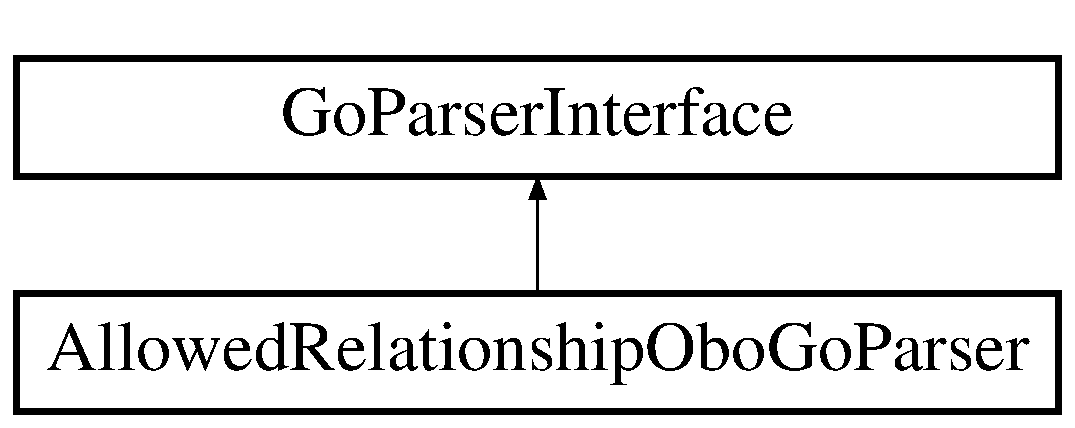
\includegraphics[height=2.000000cm]{classAllowedRelationshipOboGoParser}
\end{center}
\end{figure}
\subsection*{Public Member Functions}
\begin{DoxyCompactItemize}
\item 
\hyperlink{classGoGraph}{Go\+Graph} $\ast$ \hyperlink{classAllowedRelationshipOboGoParser_a6eb0ab84216c386a2595aa47233448ad}{parse\+Go\+File} (std\+::string filename)
\begin{DoxyCompactList}\small\item\em Method to parse the go file, should be an O\+BO file. \end{DoxyCompactList}\item 
bool \hyperlink{classAllowedRelationshipOboGoParser_a67722c03da0ca2e0f9eb4008dddc6e06}{is\+File\+Good} (const std\+::string \&filename)
\begin{DoxyCompactList}\small\item\em A method to test if a file fits the accepted format. \end{DoxyCompactList}\item 
void \hyperlink{classAllowedRelationshipOboGoParser_a675bd9d5e302fe77b96e16ef647e53d1}{split\+With} (const std\+::string \&instr, const std\+::string \&split\+Str, std\+::string \&attr, std\+::string \&value)
\begin{DoxyCompactList}\small\item\em a helper method \end{DoxyCompactList}\item 
\hyperlink{classGoParserInterface}{Go\+Parser\+Interface} $\ast$ \hyperlink{classAllowedRelationshipOboGoParser_add9a434ad4acd785b51550dc5fd9388b}{clone} ()
\begin{DoxyCompactList}\small\item\em a method to create a new instance of this class for use in a factory \end{DoxyCompactList}\item 
void \hyperlink{classAllowedRelationshipOboGoParser_ab232a6b864dc4350f95da6f281df4491}{set\+Policy} (\hyperlink{classRelationshipPolicyInterface}{Relationship\+Policy\+Interface} $\ast$policy)
\begin{DoxyCompactList}\small\item\em a method to set the policy \end{DoxyCompactList}\item 
\hyperlink{classAllowedRelationshipOboGoParser_ac74305e8723b42f6c6ffd78ff4c9824e}{Allowed\+Relationship\+Obo\+Go\+Parser} (\hyperlink{classRelationshipPolicyInterface}{Relationship\+Policy\+Interface} $\ast$policy)
\begin{DoxyCompactList}\small\item\em A parameterized constructor. \end{DoxyCompactList}\end{DoxyCompactItemize}


\subsection{Detailed Description}
A class to parse only a specified set of relationships. 

This class will read a Gene Ontology O\+BO file and add only those relationship which are specified to the graph. The most important method of this class if the parse\+Go\+File which takes the file name as a parameter.

Implements \hyperlink{classGoParserInterface}{Go\+Parser\+Interface} 

\subsection{Constructor \& Destructor Documentation}
\index{Allowed\+Relationship\+Obo\+Go\+Parser@{Allowed\+Relationship\+Obo\+Go\+Parser}!Allowed\+Relationship\+Obo\+Go\+Parser@{Allowed\+Relationship\+Obo\+Go\+Parser}}
\index{Allowed\+Relationship\+Obo\+Go\+Parser@{Allowed\+Relationship\+Obo\+Go\+Parser}!Allowed\+Relationship\+Obo\+Go\+Parser@{Allowed\+Relationship\+Obo\+Go\+Parser}}
\subsubsection[{\texorpdfstring{Allowed\+Relationship\+Obo\+Go\+Parser(\+Relationship\+Policy\+Interface $\ast$policy)}{AllowedRelationshipOboGoParser(RelationshipPolicyInterface *policy)}}]{\setlength{\rightskip}{0pt plus 5cm}Allowed\+Relationship\+Obo\+Go\+Parser\+::\+Allowed\+Relationship\+Obo\+Go\+Parser (
\begin{DoxyParamCaption}
\item[{{\bf Relationship\+Policy\+Interface} $\ast$}]{policy}
\end{DoxyParamCaption}
)\hspace{0.3cm}{\ttfamily [inline]}}\hypertarget{classAllowedRelationshipOboGoParser_ac74305e8723b42f6c6ffd78ff4c9824e}{}\label{classAllowedRelationshipOboGoParser_ac74305e8723b42f6c6ffd78ff4c9824e}


A parameterized constructor. 

constructor that sets the policy 

\subsection{Member Function Documentation}
\index{Allowed\+Relationship\+Obo\+Go\+Parser@{Allowed\+Relationship\+Obo\+Go\+Parser}!clone@{clone}}
\index{clone@{clone}!Allowed\+Relationship\+Obo\+Go\+Parser@{Allowed\+Relationship\+Obo\+Go\+Parser}}
\subsubsection[{\texorpdfstring{clone()}{clone()}}]{\setlength{\rightskip}{0pt plus 5cm}{\bf Go\+Parser\+Interface}$\ast$ Allowed\+Relationship\+Obo\+Go\+Parser\+::clone (
\begin{DoxyParamCaption}
{}
\end{DoxyParamCaption}
)\hspace{0.3cm}{\ttfamily [inline]}, {\ttfamily [virtual]}}\hypertarget{classAllowedRelationshipOboGoParser_add9a434ad4acd785b51550dc5fd9388b}{}\label{classAllowedRelationshipOboGoParser_add9a434ad4acd785b51550dc5fd9388b}


a method to create a new instance of this class for use in a factory 

creats a new pointer to the parser, used by the factory for go parsers. 

Implements \hyperlink{classGoParserInterface_a21c4ea01809737ab2975fb71edf6fcd5}{Go\+Parser\+Interface}.

\index{Allowed\+Relationship\+Obo\+Go\+Parser@{Allowed\+Relationship\+Obo\+Go\+Parser}!is\+File\+Good@{is\+File\+Good}}
\index{is\+File\+Good@{is\+File\+Good}!Allowed\+Relationship\+Obo\+Go\+Parser@{Allowed\+Relationship\+Obo\+Go\+Parser}}
\subsubsection[{\texorpdfstring{is\+File\+Good(const std\+::string \&filename)}{isFileGood(const std::string &filename)}}]{\setlength{\rightskip}{0pt plus 5cm}bool Allowed\+Relationship\+Obo\+Go\+Parser\+::is\+File\+Good (
\begin{DoxyParamCaption}
\item[{const std\+::string \&}]{filename}
\end{DoxyParamCaption}
)\hspace{0.3cm}{\ttfamily [inline]}, {\ttfamily [virtual]}}\hypertarget{classAllowedRelationshipOboGoParser_a67722c03da0ca2e0f9eb4008dddc6e06}{}\label{classAllowedRelationshipOboGoParser_a67722c03da0ca2e0f9eb4008dddc6e06}


A method to test if a file fits the accepted format. 

Returns true if the file matches accepted format, false otherwise 

Implements \hyperlink{classGoParserInterface_a0d2db54063c1ff58a0e15f0187af5aa1}{Go\+Parser\+Interface}.

\index{Allowed\+Relationship\+Obo\+Go\+Parser@{Allowed\+Relationship\+Obo\+Go\+Parser}!parse\+Go\+File@{parse\+Go\+File}}
\index{parse\+Go\+File@{parse\+Go\+File}!Allowed\+Relationship\+Obo\+Go\+Parser@{Allowed\+Relationship\+Obo\+Go\+Parser}}
\subsubsection[{\texorpdfstring{parse\+Go\+File(std\+::string filename)}{parseGoFile(std::string filename)}}]{\setlength{\rightskip}{0pt plus 5cm}{\bf Go\+Graph}$\ast$ Allowed\+Relationship\+Obo\+Go\+Parser\+::parse\+Go\+File (
\begin{DoxyParamCaption}
\item[{std\+::string}]{filename}
\end{DoxyParamCaption}
)\hspace{0.3cm}{\ttfamily [inline]}, {\ttfamily [virtual]}}\hypertarget{classAllowedRelationshipOboGoParser_a6eb0ab84216c386a2595aa47233448ad}{}\label{classAllowedRelationshipOboGoParser_a6eb0ab84216c386a2595aa47233448ad}


Method to parse the go file, should be an O\+BO file. 

This method will read a Gene Ontology O\+BO file and add only those relationship which are specified to the graph. 

Implements \hyperlink{classGoParserInterface_aefde440e0d5404b9efa2a16a89e09674}{Go\+Parser\+Interface}.

\index{Allowed\+Relationship\+Obo\+Go\+Parser@{Allowed\+Relationship\+Obo\+Go\+Parser}!set\+Policy@{set\+Policy}}
\index{set\+Policy@{set\+Policy}!Allowed\+Relationship\+Obo\+Go\+Parser@{Allowed\+Relationship\+Obo\+Go\+Parser}}
\subsubsection[{\texorpdfstring{set\+Policy(\+Relationship\+Policy\+Interface $\ast$policy)}{setPolicy(RelationshipPolicyInterface *policy)}}]{\setlength{\rightskip}{0pt plus 5cm}void Allowed\+Relationship\+Obo\+Go\+Parser\+::set\+Policy (
\begin{DoxyParamCaption}
\item[{{\bf Relationship\+Policy\+Interface} $\ast$}]{policy}
\end{DoxyParamCaption}
)\hspace{0.3cm}{\ttfamily [inline]}}\hypertarget{classAllowedRelationshipOboGoParser_ab232a6b864dc4350f95da6f281df4491}{}\label{classAllowedRelationshipOboGoParser_ab232a6b864dc4350f95da6f281df4491}


a method to set the policy 

sets the policy of the parser \index{Allowed\+Relationship\+Obo\+Go\+Parser@{Allowed\+Relationship\+Obo\+Go\+Parser}!split\+With@{split\+With}}
\index{split\+With@{split\+With}!Allowed\+Relationship\+Obo\+Go\+Parser@{Allowed\+Relationship\+Obo\+Go\+Parser}}
\subsubsection[{\texorpdfstring{split\+With(const std\+::string \&instr, const std\+::string \&split\+Str, std\+::string \&attr, std\+::string \&value)}{splitWith(const std::string &instr, const std::string &splitStr, std::string &attr, std::string &value)}}]{\setlength{\rightskip}{0pt plus 5cm}void Allowed\+Relationship\+Obo\+Go\+Parser\+::split\+With (
\begin{DoxyParamCaption}
\item[{const std\+::string \&}]{instr, }
\item[{const std\+::string \&}]{split\+Str, }
\item[{std\+::string \&}]{attr, }
\item[{std\+::string \&}]{value}
\end{DoxyParamCaption}
)\hspace{0.3cm}{\ttfamily [inline]}}\hypertarget{classAllowedRelationshipOboGoParser_a675bd9d5e302fe77b96e16ef647e53d1}{}\label{classAllowedRelationshipOboGoParser_a675bd9d5e302fe77b96e16ef647e53d1}


a helper method 

splits strings on the given string pattern, split\+Str. 

The documentation for this class was generated from the following file\+:\begin{DoxyCompactItemize}
\item 
ggtk/Allowed\+Relationship\+Obo\+Go\+Parser.\+hpp\end{DoxyCompactItemize}

\hypertarget{classAllowedRelationshipXmlGoParser}{}\section{Allowed\+Relationship\+Xml\+Go\+Parser Class Reference}
\label{classAllowedRelationshipXmlGoParser}\index{Allowed\+Relationship\+Xml\+Go\+Parser@{Allowed\+Relationship\+Xml\+Go\+Parser}}


A class to parse only a specified set of relationships.  




{\ttfamily \#include $<$ggtk/\+Allowed\+Relationship\+Xml\+Go\+Parser.\+hpp$>$}

Inheritance diagram for Allowed\+Relationship\+Xml\+Go\+Parser\+:\begin{figure}[H]
\begin{center}
\leavevmode
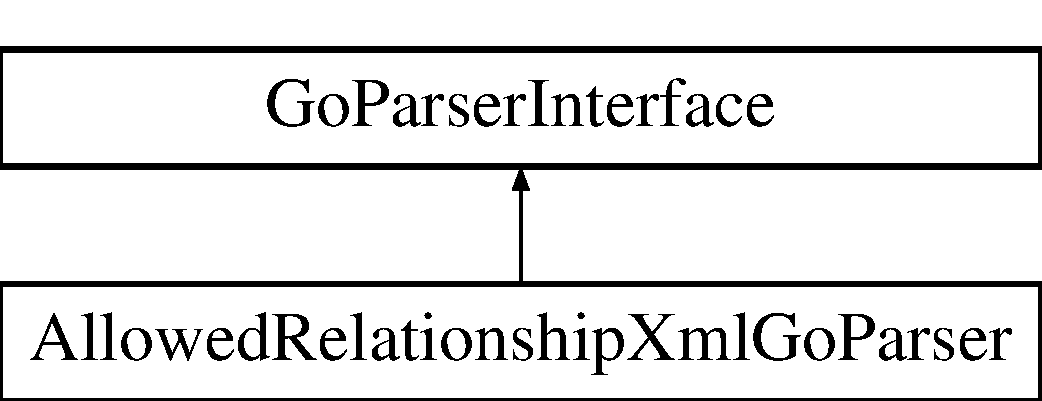
\includegraphics[height=2.000000cm]{classAllowedRelationshipXmlGoParser}
\end{center}
\end{figure}
\subsection*{Public Member Functions}
\begin{DoxyCompactItemize}
\item 
\hyperlink{classGoGraph}{Go\+Graph} $\ast$ \hyperlink{classAllowedRelationshipXmlGoParser_ad6e002e7cd0994866b62dba0896d3d24}{parse\+Go\+File} (std\+::string filename)
\begin{DoxyCompactList}\small\item\em Method to parse the go file, should be an X\+ML file. \end{DoxyCompactList}\item 
bool \hyperlink{classAllowedRelationshipXmlGoParser_a75e964bc34f575bc6c00c56b43f91d0e}{is\+File\+Good} (const std\+::string \&filename)
\begin{DoxyCompactList}\small\item\em A method to test if a file fits the accepted format. \end{DoxyCompactList}\item 
\hyperlink{classGoParserInterface}{Go\+Parser\+Interface} $\ast$ \hyperlink{classAllowedRelationshipXmlGoParser_a3c330bc9f1ccf6422488bf1ea593f52a}{clone} ()
\begin{DoxyCompactList}\small\item\em a method to create a new instance of this class for use in a factory \end{DoxyCompactList}\item 
void \hyperlink{classAllowedRelationshipXmlGoParser_a463df4ceee68bf1321c982812f77eed2}{set\+Policy} (\hyperlink{classRelationshipPolicyInterface}{Relationship\+Policy\+Interface} $\ast$policy)
\begin{DoxyCompactList}\small\item\em a method to set the policy \end{DoxyCompactList}\item 
\hyperlink{classAllowedRelationshipXmlGoParser_a51bd1af3274c80d1600e0f3b88815ef4}{Allowed\+Relationship\+Xml\+Go\+Parser} (\hyperlink{classRelationshipPolicyInterface}{Relationship\+Policy\+Interface} $\ast$policy)
\begin{DoxyCompactList}\small\item\em A parameterized constructor. \end{DoxyCompactList}\end{DoxyCompactItemize}


\subsection{Detailed Description}
A class to parse only a specified set of relationships. 

This class will read a Gene Ontology X\+ML file and add only those relationship which are specified to the graph. The most important method of this class if the parse\+Go\+File which takes the file name as a parameter.

Implements \hyperlink{classGoParserInterface}{Go\+Parser\+Interface} 

\subsection{Constructor \& Destructor Documentation}
\index{Allowed\+Relationship\+Xml\+Go\+Parser@{Allowed\+Relationship\+Xml\+Go\+Parser}!Allowed\+Relationship\+Xml\+Go\+Parser@{Allowed\+Relationship\+Xml\+Go\+Parser}}
\index{Allowed\+Relationship\+Xml\+Go\+Parser@{Allowed\+Relationship\+Xml\+Go\+Parser}!Allowed\+Relationship\+Xml\+Go\+Parser@{Allowed\+Relationship\+Xml\+Go\+Parser}}
\subsubsection[{\texorpdfstring{Allowed\+Relationship\+Xml\+Go\+Parser(\+Relationship\+Policy\+Interface $\ast$policy)}{AllowedRelationshipXmlGoParser(RelationshipPolicyInterface *policy)}}]{\setlength{\rightskip}{0pt plus 5cm}Allowed\+Relationship\+Xml\+Go\+Parser\+::\+Allowed\+Relationship\+Xml\+Go\+Parser (
\begin{DoxyParamCaption}
\item[{{\bf Relationship\+Policy\+Interface} $\ast$}]{policy}
\end{DoxyParamCaption}
)\hspace{0.3cm}{\ttfamily [inline]}}\hypertarget{classAllowedRelationshipXmlGoParser_a51bd1af3274c80d1600e0f3b88815ef4}{}\label{classAllowedRelationshipXmlGoParser_a51bd1af3274c80d1600e0f3b88815ef4}


A parameterized constructor. 

constructor that sets the policy 

\subsection{Member Function Documentation}
\index{Allowed\+Relationship\+Xml\+Go\+Parser@{Allowed\+Relationship\+Xml\+Go\+Parser}!clone@{clone}}
\index{clone@{clone}!Allowed\+Relationship\+Xml\+Go\+Parser@{Allowed\+Relationship\+Xml\+Go\+Parser}}
\subsubsection[{\texorpdfstring{clone()}{clone()}}]{\setlength{\rightskip}{0pt plus 5cm}{\bf Go\+Parser\+Interface}$\ast$ Allowed\+Relationship\+Xml\+Go\+Parser\+::clone (
\begin{DoxyParamCaption}
{}
\end{DoxyParamCaption}
)\hspace{0.3cm}{\ttfamily [inline]}, {\ttfamily [virtual]}}\hypertarget{classAllowedRelationshipXmlGoParser_a3c330bc9f1ccf6422488bf1ea593f52a}{}\label{classAllowedRelationshipXmlGoParser_a3c330bc9f1ccf6422488bf1ea593f52a}


a method to create a new instance of this class for use in a factory 

creats a new pointer to the parser, used by the factory for go parsers. 

Implements \hyperlink{classGoParserInterface_a21c4ea01809737ab2975fb71edf6fcd5}{Go\+Parser\+Interface}.

\index{Allowed\+Relationship\+Xml\+Go\+Parser@{Allowed\+Relationship\+Xml\+Go\+Parser}!is\+File\+Good@{is\+File\+Good}}
\index{is\+File\+Good@{is\+File\+Good}!Allowed\+Relationship\+Xml\+Go\+Parser@{Allowed\+Relationship\+Xml\+Go\+Parser}}
\subsubsection[{\texorpdfstring{is\+File\+Good(const std\+::string \&filename)}{isFileGood(const std::string &filename)}}]{\setlength{\rightskip}{0pt plus 5cm}bool Allowed\+Relationship\+Xml\+Go\+Parser\+::is\+File\+Good (
\begin{DoxyParamCaption}
\item[{const std\+::string \&}]{filename}
\end{DoxyParamCaption}
)\hspace{0.3cm}{\ttfamily [inline]}, {\ttfamily [virtual]}}\hypertarget{classAllowedRelationshipXmlGoParser_a75e964bc34f575bc6c00c56b43f91d0e}{}\label{classAllowedRelationshipXmlGoParser_a75e964bc34f575bc6c00c56b43f91d0e}


A method to test if a file fits the accepted format. 

Returns true if the file matches accepted format, false otherwise 

Implements \hyperlink{classGoParserInterface_a0d2db54063c1ff58a0e15f0187af5aa1}{Go\+Parser\+Interface}.

\index{Allowed\+Relationship\+Xml\+Go\+Parser@{Allowed\+Relationship\+Xml\+Go\+Parser}!parse\+Go\+File@{parse\+Go\+File}}
\index{parse\+Go\+File@{parse\+Go\+File}!Allowed\+Relationship\+Xml\+Go\+Parser@{Allowed\+Relationship\+Xml\+Go\+Parser}}
\subsubsection[{\texorpdfstring{parse\+Go\+File(std\+::string filename)}{parseGoFile(std::string filename)}}]{\setlength{\rightskip}{0pt plus 5cm}{\bf Go\+Graph}$\ast$ Allowed\+Relationship\+Xml\+Go\+Parser\+::parse\+Go\+File (
\begin{DoxyParamCaption}
\item[{std\+::string}]{filename}
\end{DoxyParamCaption}
)\hspace{0.3cm}{\ttfamily [inline]}, {\ttfamily [virtual]}}\hypertarget{classAllowedRelationshipXmlGoParser_ad6e002e7cd0994866b62dba0896d3d24}{}\label{classAllowedRelationshipXmlGoParser_ad6e002e7cd0994866b62dba0896d3d24}


Method to parse the go file, should be an X\+ML file. 

This method will read a Gene Ontology X\+ML file and add only those relationship which are specified to the graph. 

Implements \hyperlink{classGoParserInterface_aefde440e0d5404b9efa2a16a89e09674}{Go\+Parser\+Interface}.

\index{Allowed\+Relationship\+Xml\+Go\+Parser@{Allowed\+Relationship\+Xml\+Go\+Parser}!set\+Policy@{set\+Policy}}
\index{set\+Policy@{set\+Policy}!Allowed\+Relationship\+Xml\+Go\+Parser@{Allowed\+Relationship\+Xml\+Go\+Parser}}
\subsubsection[{\texorpdfstring{set\+Policy(\+Relationship\+Policy\+Interface $\ast$policy)}{setPolicy(RelationshipPolicyInterface *policy)}}]{\setlength{\rightskip}{0pt plus 5cm}void Allowed\+Relationship\+Xml\+Go\+Parser\+::set\+Policy (
\begin{DoxyParamCaption}
\item[{{\bf Relationship\+Policy\+Interface} $\ast$}]{policy}
\end{DoxyParamCaption}
)\hspace{0.3cm}{\ttfamily [inline]}}\hypertarget{classAllowedRelationshipXmlGoParser_a463df4ceee68bf1321c982812f77eed2}{}\label{classAllowedRelationshipXmlGoParser_a463df4ceee68bf1321c982812f77eed2}


a method to set the policy 

sets the policy of the parser 

The documentation for this class was generated from the following file\+:\begin{DoxyCompactItemize}
\item 
ggtk/Allowed\+Relationship\+Xml\+Go\+Parser.\+hpp\end{DoxyCompactItemize}

\hypertarget{classAllowedSetEvidencePolicy}{}\section{Allowed\+Set\+Evidence\+Policy Class Reference}
\label{classAllowedSetEvidencePolicy}\index{Allowed\+Set\+Evidence\+Policy@{Allowed\+Set\+Evidence\+Policy}}


A class to allow only a set of evidence codes for annotations.  




{\ttfamily \#include $<$ggtk/\+Allowed\+Set\+Evidence\+Policy.\+hpp$>$}

Inheritance diagram for Allowed\+Set\+Evidence\+Policy\+:\begin{figure}[H]
\begin{center}
\leavevmode
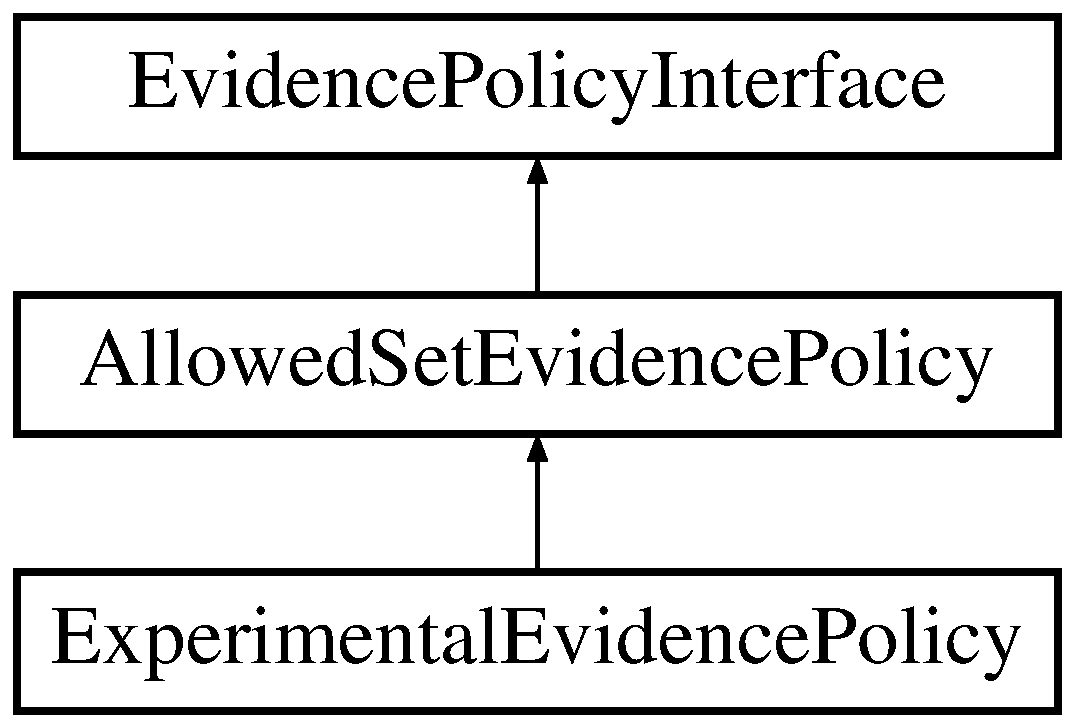
\includegraphics[height=3.000000cm]{classAllowedSetEvidencePolicy}
\end{center}
\end{figure}
\subsection*{Public Member Functions}
\begin{DoxyCompactItemize}
\item 
\hyperlink{classAllowedSetEvidencePolicy_af940574b5c998db67ce580555e1964d3}{Allowed\+Set\+Evidence\+Policy} ()
\begin{DoxyCompactList}\small\item\em A constructor. \end{DoxyCompactList}\item 
\hyperlink{classAllowedSetEvidencePolicy_a84458d133059ab286b3d3eaa8301d243}{Allowed\+Set\+Evidence\+Policy} (std\+::vector$<$ \hyperlink{namespaceGO_a4ce5387bbcdaec3648957c7903f2caf3}{G\+O\+::\+Evidence\+Code} $>$ evidence\+Codes)
\begin{DoxyCompactList}\small\item\em A parameterized constructor. \end{DoxyCompactList}\item 
bool \hyperlink{classAllowedSetEvidencePolicy_a5979a55da22e57d2faffaa0bdb77457b}{is\+Allowed} (\hyperlink{namespaceGO_a4ce5387bbcdaec3648957c7903f2caf3}{G\+O\+::\+Evidence\+Code} evidence\+Code)
\begin{DoxyCompactList}\small\item\em a method to test if an eviddence code is allowed or not \end{DoxyCompactList}\item 
void \hyperlink{classAllowedSetEvidencePolicy_a8a68cd6a472cab9df1dda7b3258618cf}{add\+Evidence} (\hyperlink{namespaceGO_a4ce5387bbcdaec3648957c7903f2caf3}{G\+O\+::\+Evidence\+Code} evidence\+Code)
\begin{DoxyCompactList}\small\item\em a method to add a evidence to the set of evidence codes allowed \end{DoxyCompactList}\item 
void \hyperlink{classAllowedSetEvidencePolicy_a1013d74c48b800c7dd0450c0fdaa4090}{add\+Evidence} (const std\+::string \&string\+Code)
\begin{DoxyCompactList}\small\item\em a method to add a evidence to the set of evidence codes allowed \end{DoxyCompactList}\item 
bool \hyperlink{classAllowedSetEvidencePolicy_ac54f499b3dfd0a55353014f1f277fe64}{is\+Empty} ()
\begin{DoxyCompactList}\small\item\em a method to determine if the Policy is empty \end{DoxyCompactList}\end{DoxyCompactItemize}


\subsection{Detailed Description}
A class to allow only a set of evidence codes for annotations. 

A class to allow only certain evidence codes in the go graph. It uses a set of enums to restric the types of evidence codes considered for annotations. 

\subsection{Constructor \& Destructor Documentation}
\index{Allowed\+Set\+Evidence\+Policy@{Allowed\+Set\+Evidence\+Policy}!Allowed\+Set\+Evidence\+Policy@{Allowed\+Set\+Evidence\+Policy}}
\index{Allowed\+Set\+Evidence\+Policy@{Allowed\+Set\+Evidence\+Policy}!Allowed\+Set\+Evidence\+Policy@{Allowed\+Set\+Evidence\+Policy}}
\subsubsection[{\texorpdfstring{Allowed\+Set\+Evidence\+Policy()}{AllowedSetEvidencePolicy()}}]{\setlength{\rightskip}{0pt plus 5cm}Allowed\+Set\+Evidence\+Policy\+::\+Allowed\+Set\+Evidence\+Policy (
\begin{DoxyParamCaption}
{}
\end{DoxyParamCaption}
)\hspace{0.3cm}{\ttfamily [inline]}}\hypertarget{classAllowedSetEvidencePolicy_af940574b5c998db67ce580555e1964d3}{}\label{classAllowedSetEvidencePolicy_af940574b5c998db67ce580555e1964d3}


A constructor. 

Creates the default(empty) \hyperlink{classAllowedSetEvidencePolicy}{Allowed\+Set\+Evidence\+Policy} \index{Allowed\+Set\+Evidence\+Policy@{Allowed\+Set\+Evidence\+Policy}!Allowed\+Set\+Evidence\+Policy@{Allowed\+Set\+Evidence\+Policy}}
\index{Allowed\+Set\+Evidence\+Policy@{Allowed\+Set\+Evidence\+Policy}!Allowed\+Set\+Evidence\+Policy@{Allowed\+Set\+Evidence\+Policy}}
\subsubsection[{\texorpdfstring{Allowed\+Set\+Evidence\+Policy(std\+::vector$<$ G\+O\+::\+Evidence\+Code $>$ evidence\+Codes)}{AllowedSetEvidencePolicy(std::vector< GO::EvidenceCode > evidenceCodes)}}]{\setlength{\rightskip}{0pt plus 5cm}Allowed\+Set\+Evidence\+Policy\+::\+Allowed\+Set\+Evidence\+Policy (
\begin{DoxyParamCaption}
\item[{std\+::vector$<$ {\bf G\+O\+::\+Evidence\+Code} $>$}]{evidence\+Codes}
\end{DoxyParamCaption}
)\hspace{0.3cm}{\ttfamily [inline]}}\hypertarget{classAllowedSetEvidencePolicy_a84458d133059ab286b3d3eaa8301d243}{}\label{classAllowedSetEvidencePolicy_a84458d133059ab286b3d3eaa8301d243}


A parameterized constructor. 

Creats the \hyperlink{classAllowedSetEvidencePolicy}{Allowed\+Set\+Evidence\+Policy} using a list(vector) of evidence codes to allow 

\subsection{Member Function Documentation}
\index{Allowed\+Set\+Evidence\+Policy@{Allowed\+Set\+Evidence\+Policy}!add\+Evidence@{add\+Evidence}}
\index{add\+Evidence@{add\+Evidence}!Allowed\+Set\+Evidence\+Policy@{Allowed\+Set\+Evidence\+Policy}}
\subsubsection[{\texorpdfstring{add\+Evidence(\+G\+O\+::\+Evidence\+Code evidence\+Code)}{addEvidence(GO::EvidenceCode evidenceCode)}}]{\setlength{\rightskip}{0pt plus 5cm}void Allowed\+Set\+Evidence\+Policy\+::add\+Evidence (
\begin{DoxyParamCaption}
\item[{{\bf G\+O\+::\+Evidence\+Code}}]{evidence\+Code}
\end{DoxyParamCaption}
)\hspace{0.3cm}{\ttfamily [inline]}}\hypertarget{classAllowedSetEvidencePolicy_a8a68cd6a472cab9df1dda7b3258618cf}{}\label{classAllowedSetEvidencePolicy_a8a68cd6a472cab9df1dda7b3258618cf}


a method to add a evidence to the set of evidence codes allowed 

adds a evidence to the set of evidence codes allowed by setting its mapped value to true \index{Allowed\+Set\+Evidence\+Policy@{Allowed\+Set\+Evidence\+Policy}!add\+Evidence@{add\+Evidence}}
\index{add\+Evidence@{add\+Evidence}!Allowed\+Set\+Evidence\+Policy@{Allowed\+Set\+Evidence\+Policy}}
\subsubsection[{\texorpdfstring{add\+Evidence(const std\+::string \&string\+Code)}{addEvidence(const std::string &stringCode)}}]{\setlength{\rightskip}{0pt plus 5cm}void Allowed\+Set\+Evidence\+Policy\+::add\+Evidence (
\begin{DoxyParamCaption}
\item[{const std\+::string \&}]{string\+Code}
\end{DoxyParamCaption}
)\hspace{0.3cm}{\ttfamily [inline]}}\hypertarget{classAllowedSetEvidencePolicy_a1013d74c48b800c7dd0450c0fdaa4090}{}\label{classAllowedSetEvidencePolicy_a1013d74c48b800c7dd0450c0fdaa4090}


a method to add a evidence to the set of evidence codes allowed 

adds a evidence to the set of evidence codes allowed by setting its mapped value to true \index{Allowed\+Set\+Evidence\+Policy@{Allowed\+Set\+Evidence\+Policy}!is\+Allowed@{is\+Allowed}}
\index{is\+Allowed@{is\+Allowed}!Allowed\+Set\+Evidence\+Policy@{Allowed\+Set\+Evidence\+Policy}}
\subsubsection[{\texorpdfstring{is\+Allowed(\+G\+O\+::\+Evidence\+Code evidence\+Code)}{isAllowed(GO::EvidenceCode evidenceCode)}}]{\setlength{\rightskip}{0pt plus 5cm}bool Allowed\+Set\+Evidence\+Policy\+::is\+Allowed (
\begin{DoxyParamCaption}
\item[{{\bf G\+O\+::\+Evidence\+Code}}]{evidence\+Code}
\end{DoxyParamCaption}
)\hspace{0.3cm}{\ttfamily [inline]}, {\ttfamily [virtual]}}\hypertarget{classAllowedSetEvidencePolicy_a5979a55da22e57d2faffaa0bdb77457b}{}\label{classAllowedSetEvidencePolicy_a5979a55da22e57d2faffaa0bdb77457b}


a method to test if an eviddence code is allowed or not 

tests if the evidence is allowed. Overridden to fulfill the \hyperlink{classEvidencePolicyInterface}{Evidence\+Policy\+Interface} 

Implements \hyperlink{classEvidencePolicyInterface_a432d20dd05ec54db46a452ae8d6be4a7}{Evidence\+Policy\+Interface}.

\index{Allowed\+Set\+Evidence\+Policy@{Allowed\+Set\+Evidence\+Policy}!is\+Empty@{is\+Empty}}
\index{is\+Empty@{is\+Empty}!Allowed\+Set\+Evidence\+Policy@{Allowed\+Set\+Evidence\+Policy}}
\subsubsection[{\texorpdfstring{is\+Empty()}{isEmpty()}}]{\setlength{\rightskip}{0pt plus 5cm}bool Allowed\+Set\+Evidence\+Policy\+::is\+Empty (
\begin{DoxyParamCaption}
{}
\end{DoxyParamCaption}
)\hspace{0.3cm}{\ttfamily [inline]}}\hypertarget{classAllowedSetEvidencePolicy_ac54f499b3dfd0a55353014f1f277fe64}{}\label{classAllowedSetEvidencePolicy_ac54f499b3dfd0a55353014f1f277fe64}


a method to determine if the Policy is empty 

Determines if the Policy is empty 

The documentation for this class was generated from the following file\+:\begin{DoxyCompactItemize}
\item 
ggtk/Allowed\+Set\+Evidence\+Policy.\+hpp\end{DoxyCompactItemize}

\hypertarget{classAllowedSetRelationshipPolicy}{}\section{Allowed\+Set\+Relationship\+Policy Class Reference}
\label{classAllowedSetRelationshipPolicy}\index{Allowed\+Set\+Relationship\+Policy@{Allowed\+Set\+Relationship\+Policy}}


A class to allow only a set of relationships.  




{\ttfamily \#include $<$ggtk/\+Allowed\+Set\+Relationship\+Policy.\+hpp$>$}

Inheritance diagram for Allowed\+Set\+Relationship\+Policy\+:\begin{figure}[H]
\begin{center}
\leavevmode
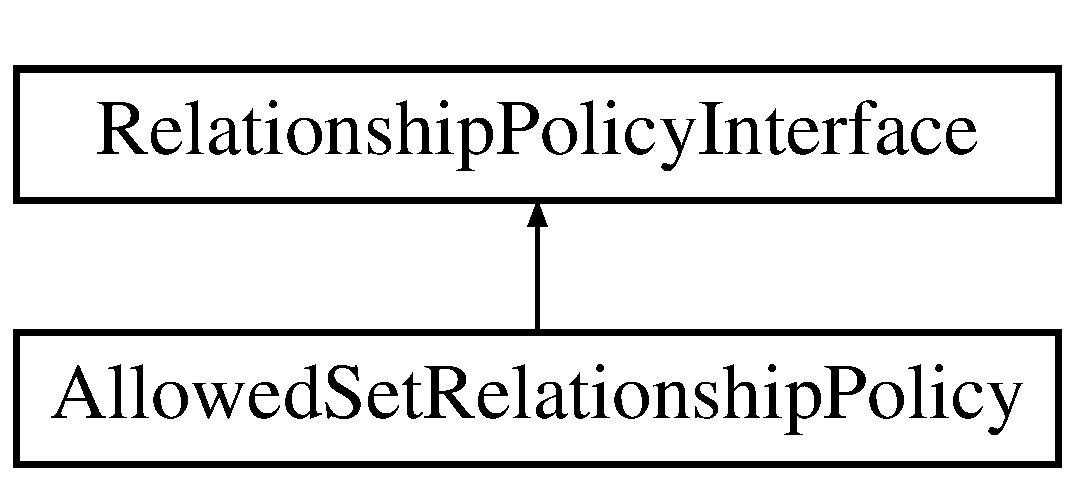
\includegraphics[height=2.000000cm]{classAllowedSetRelationshipPolicy}
\end{center}
\end{figure}
\subsection*{Public Member Functions}
\begin{DoxyCompactItemize}
\item 
\hyperlink{classAllowedSetRelationshipPolicy_aebffb7e69930219d89133625ff8936cf}{Allowed\+Set\+Relationship\+Policy} ()
\begin{DoxyCompactList}\small\item\em A constructor. \end{DoxyCompactList}\item 
\hyperlink{classAllowedSetRelationshipPolicy_a9cd20d2c44a96736c0a74b7e962dae04}{Allowed\+Set\+Relationship\+Policy} (std\+::vector$<$ \hyperlink{namespaceGO_aaa3905b2e000a8be411da8038827f993}{G\+O\+::\+Relationship} $>$ relationships)
\begin{DoxyCompactList}\small\item\em A parameterized constructor. \end{DoxyCompactList}\item 
bool \hyperlink{classAllowedSetRelationshipPolicy_ac7454bc649241219f076779330977f90}{is\+Allowed} (\hyperlink{namespaceGO_aaa3905b2e000a8be411da8038827f993}{G\+O\+::\+Relationship} relationship)
\begin{DoxyCompactList}\small\item\em a method to test if a relatinoship is allowed or not \end{DoxyCompactList}\item 
void \hyperlink{classAllowedSetRelationshipPolicy_a5da8f3fb718fba44354e56a4595968de}{add\+Relationship} (\hyperlink{namespaceGO_aaa3905b2e000a8be411da8038827f993}{G\+O\+::\+Relationship} relationship)
\begin{DoxyCompactList}\small\item\em a method to add a relationship to the set of relationships allowed \end{DoxyCompactList}\item 
void \hyperlink{classAllowedSetRelationshipPolicy_a013089769911f87f1d8513bc6006dbf9}{add\+Relationship} (const std\+::string \&rel\+String)
\begin{DoxyCompactList}\small\item\em a method to add a relationship to the set of relationships allowed \end{DoxyCompactList}\item 
bool \hyperlink{classAllowedSetRelationshipPolicy_a543f028def505d8df941a308ab315075}{is\+Empty} ()
\begin{DoxyCompactList}\small\item\em a method to determine if the Policy is empty \end{DoxyCompactList}\end{DoxyCompactItemize}


\subsection{Detailed Description}
A class to allow only a set of relationships. 

A class to allow only certain relationships in the go graph. It uses a set of enums to restric the types of relationships considered in a graph. 

\subsection{Constructor \& Destructor Documentation}
\index{Allowed\+Set\+Relationship\+Policy@{Allowed\+Set\+Relationship\+Policy}!Allowed\+Set\+Relationship\+Policy@{Allowed\+Set\+Relationship\+Policy}}
\index{Allowed\+Set\+Relationship\+Policy@{Allowed\+Set\+Relationship\+Policy}!Allowed\+Set\+Relationship\+Policy@{Allowed\+Set\+Relationship\+Policy}}
\subsubsection[{\texorpdfstring{Allowed\+Set\+Relationship\+Policy()}{AllowedSetRelationshipPolicy()}}]{\setlength{\rightskip}{0pt plus 5cm}Allowed\+Set\+Relationship\+Policy\+::\+Allowed\+Set\+Relationship\+Policy (
\begin{DoxyParamCaption}
{}
\end{DoxyParamCaption}
)\hspace{0.3cm}{\ttfamily [inline]}}\hypertarget{classAllowedSetRelationshipPolicy_aebffb7e69930219d89133625ff8936cf}{}\label{classAllowedSetRelationshipPolicy_aebffb7e69930219d89133625ff8936cf}


A constructor. 

Creates the default(empty) \hyperlink{classAllowedSetRelationshipPolicy}{Allowed\+Set\+Relationship\+Policy} \index{Allowed\+Set\+Relationship\+Policy@{Allowed\+Set\+Relationship\+Policy}!Allowed\+Set\+Relationship\+Policy@{Allowed\+Set\+Relationship\+Policy}}
\index{Allowed\+Set\+Relationship\+Policy@{Allowed\+Set\+Relationship\+Policy}!Allowed\+Set\+Relationship\+Policy@{Allowed\+Set\+Relationship\+Policy}}
\subsubsection[{\texorpdfstring{Allowed\+Set\+Relationship\+Policy(std\+::vector$<$ G\+O\+::\+Relationship $>$ relationships)}{AllowedSetRelationshipPolicy(std::vector< GO::Relationship > relationships)}}]{\setlength{\rightskip}{0pt plus 5cm}Allowed\+Set\+Relationship\+Policy\+::\+Allowed\+Set\+Relationship\+Policy (
\begin{DoxyParamCaption}
\item[{std\+::vector$<$ {\bf G\+O\+::\+Relationship} $>$}]{relationships}
\end{DoxyParamCaption}
)\hspace{0.3cm}{\ttfamily [inline]}}\hypertarget{classAllowedSetRelationshipPolicy_a9cd20d2c44a96736c0a74b7e962dae04}{}\label{classAllowedSetRelationshipPolicy_a9cd20d2c44a96736c0a74b7e962dae04}


A parameterized constructor. 

Creats the \hyperlink{classAllowedSetRelationshipPolicy}{Allowed\+Set\+Relationship\+Policy} using a list(vector) of relationships to allow 

\subsection{Member Function Documentation}
\index{Allowed\+Set\+Relationship\+Policy@{Allowed\+Set\+Relationship\+Policy}!add\+Relationship@{add\+Relationship}}
\index{add\+Relationship@{add\+Relationship}!Allowed\+Set\+Relationship\+Policy@{Allowed\+Set\+Relationship\+Policy}}
\subsubsection[{\texorpdfstring{add\+Relationship(\+G\+O\+::\+Relationship relationship)}{addRelationship(GO::Relationship relationship)}}]{\setlength{\rightskip}{0pt plus 5cm}void Allowed\+Set\+Relationship\+Policy\+::add\+Relationship (
\begin{DoxyParamCaption}
\item[{{\bf G\+O\+::\+Relationship}}]{relationship}
\end{DoxyParamCaption}
)\hspace{0.3cm}{\ttfamily [inline]}}\hypertarget{classAllowedSetRelationshipPolicy_a5da8f3fb718fba44354e56a4595968de}{}\label{classAllowedSetRelationshipPolicy_a5da8f3fb718fba44354e56a4595968de}


a method to add a relationship to the set of relationships allowed 

adds a relationship to the set of relationships allowed by setting its mapped value to true \index{Allowed\+Set\+Relationship\+Policy@{Allowed\+Set\+Relationship\+Policy}!add\+Relationship@{add\+Relationship}}
\index{add\+Relationship@{add\+Relationship}!Allowed\+Set\+Relationship\+Policy@{Allowed\+Set\+Relationship\+Policy}}
\subsubsection[{\texorpdfstring{add\+Relationship(const std\+::string \&rel\+String)}{addRelationship(const std::string &relString)}}]{\setlength{\rightskip}{0pt plus 5cm}void Allowed\+Set\+Relationship\+Policy\+::add\+Relationship (
\begin{DoxyParamCaption}
\item[{const std\+::string \&}]{rel\+String}
\end{DoxyParamCaption}
)\hspace{0.3cm}{\ttfamily [inline]}}\hypertarget{classAllowedSetRelationshipPolicy_a013089769911f87f1d8513bc6006dbf9}{}\label{classAllowedSetRelationshipPolicy_a013089769911f87f1d8513bc6006dbf9}


a method to add a relationship to the set of relationships allowed 

adds a relationship to the set of relationships allowed by setting its mapped value to true \index{Allowed\+Set\+Relationship\+Policy@{Allowed\+Set\+Relationship\+Policy}!is\+Allowed@{is\+Allowed}}
\index{is\+Allowed@{is\+Allowed}!Allowed\+Set\+Relationship\+Policy@{Allowed\+Set\+Relationship\+Policy}}
\subsubsection[{\texorpdfstring{is\+Allowed(\+G\+O\+::\+Relationship relationship)}{isAllowed(GO::Relationship relationship)}}]{\setlength{\rightskip}{0pt plus 5cm}bool Allowed\+Set\+Relationship\+Policy\+::is\+Allowed (
\begin{DoxyParamCaption}
\item[{{\bf G\+O\+::\+Relationship}}]{relationship}
\end{DoxyParamCaption}
)\hspace{0.3cm}{\ttfamily [inline]}, {\ttfamily [virtual]}}\hypertarget{classAllowedSetRelationshipPolicy_ac7454bc649241219f076779330977f90}{}\label{classAllowedSetRelationshipPolicy_ac7454bc649241219f076779330977f90}


a method to test if a relatinoship is allowed or not 

tests if the relationship is allowed. Overridden to fulfill the \hyperlink{classRelationshipPolicyInterface}{Relationship\+Policy\+Interface} 

Implements \hyperlink{classRelationshipPolicyInterface_ad28012b607e9cf848c791b6a907bb2cb}{Relationship\+Policy\+Interface}.

\index{Allowed\+Set\+Relationship\+Policy@{Allowed\+Set\+Relationship\+Policy}!is\+Empty@{is\+Empty}}
\index{is\+Empty@{is\+Empty}!Allowed\+Set\+Relationship\+Policy@{Allowed\+Set\+Relationship\+Policy}}
\subsubsection[{\texorpdfstring{is\+Empty()}{isEmpty()}}]{\setlength{\rightskip}{0pt plus 5cm}bool Allowed\+Set\+Relationship\+Policy\+::is\+Empty (
\begin{DoxyParamCaption}
{}
\end{DoxyParamCaption}
)\hspace{0.3cm}{\ttfamily [inline]}}\hypertarget{classAllowedSetRelationshipPolicy_a543f028def505d8df941a308ab315075}{}\label{classAllowedSetRelationshipPolicy_a543f028def505d8df941a308ab315075}


a method to determine if the Policy is empty 

Determines if the Policy is empty 

The documentation for this class was generated from the following file\+:\begin{DoxyCompactItemize}
\item 
ggtk/Allowed\+Set\+Relationship\+Policy.\+hpp\end{DoxyCompactItemize}

\hypertarget{classAllPairsAverageSetSimilarity}{}\section{All\+Pairs\+Average\+Set\+Similarity Class Reference}
\label{classAllPairsAverageSetSimilarity}\index{All\+Pairs\+Average\+Set\+Similarity@{All\+Pairs\+Average\+Set\+Similarity}}


A class to calculate the average similarity between all pairs of go terms for 2 sets.  




{\ttfamily \#include $<$ggtk/\+All\+Pairs\+Average\+Set\+Similarity.\+hpp$>$}

Inheritance diagram for All\+Pairs\+Average\+Set\+Similarity\+:\begin{figure}[H]
\begin{center}
\leavevmode
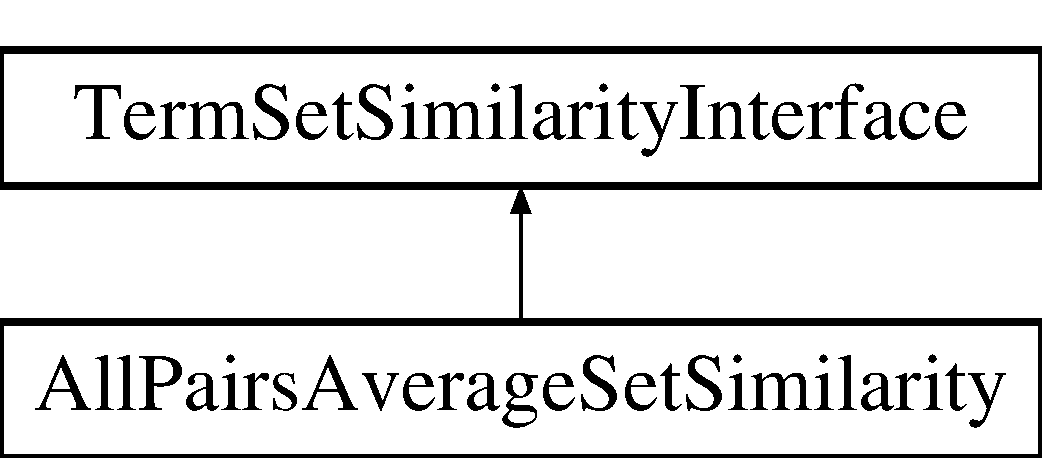
\includegraphics[height=2.000000cm]{classAllPairsAverageSetSimilarity}
\end{center}
\end{figure}
\subsection*{Public Member Functions}
\begin{DoxyCompactItemize}
\item 
\hyperlink{classAllPairsAverageSetSimilarity_a67b7cfe7f078bea616baaf99116ace2e}{All\+Pairs\+Average\+Set\+Similarity} (\hyperlink{classTermSimilarityInterface}{Term\+Similarity\+Interface} $\ast$sim\+Measure)
\begin{DoxyCompactList}\small\item\em Constructor. \end{DoxyCompactList}\item 
double \hyperlink{classAllPairsAverageSetSimilarity_a685cd98d44c2e2ab9ee4fe7071066cde}{calculate\+Similarity} (const boost\+::unordered\+\_\+set$<$ std\+::string $>$ \&termsA, const boost\+::unordered\+\_\+set$<$ std\+::string $>$ \&termsB)
\begin{DoxyCompactList}\small\item\em A method for calculating term set to term set similarity for \hyperlink{namespaceGO}{GO} terms;. \end{DoxyCompactList}\end{DoxyCompactItemize}


\subsection{Detailed Description}
A class to calculate the average similarity between all pairs of go terms for 2 sets. 

This class defines the all pairs average similarity getween two sets of terms. Put forth by Lord et al.

P. W. Lord, R. D. Stevens, A. Brass, and C. A. Goble, \char`\"{}\+Investigating semantic similarity
measures across the Gene Ontology\+: the relationship between sequence and annotation,\char`\"{} Bioinformatics, vol. 19, pp. 1275-\/83, Jul 1 2003. 

\subsection{Constructor \& Destructor Documentation}
\index{All\+Pairs\+Average\+Set\+Similarity@{All\+Pairs\+Average\+Set\+Similarity}!All\+Pairs\+Average\+Set\+Similarity@{All\+Pairs\+Average\+Set\+Similarity}}
\index{All\+Pairs\+Average\+Set\+Similarity@{All\+Pairs\+Average\+Set\+Similarity}!All\+Pairs\+Average\+Set\+Similarity@{All\+Pairs\+Average\+Set\+Similarity}}
\subsubsection[{\texorpdfstring{All\+Pairs\+Average\+Set\+Similarity(\+Term\+Similarity\+Interface $\ast$sim\+Measure)}{AllPairsAverageSetSimilarity(TermSimilarityInterface *simMeasure)}}]{\setlength{\rightskip}{0pt plus 5cm}All\+Pairs\+Average\+Set\+Similarity\+::\+All\+Pairs\+Average\+Set\+Similarity (
\begin{DoxyParamCaption}
\item[{{\bf Term\+Similarity\+Interface} $\ast$}]{sim\+Measure}
\end{DoxyParamCaption}
)\hspace{0.3cm}{\ttfamily [inline]}}\hypertarget{classAllPairsAverageSetSimilarity_a67b7cfe7f078bea616baaf99116ace2e}{}\label{classAllPairsAverageSetSimilarity_a67b7cfe7f078bea616baaf99116ace2e}


Constructor. 

Creates the \hyperlink{classAllPairsAverageSetSimilarity}{All\+Pairs\+Average\+Set\+Similarity} class assigning the similarity measure private memeber. 

\subsection{Member Function Documentation}
\index{All\+Pairs\+Average\+Set\+Similarity@{All\+Pairs\+Average\+Set\+Similarity}!calculate\+Similarity@{calculate\+Similarity}}
\index{calculate\+Similarity@{calculate\+Similarity}!All\+Pairs\+Average\+Set\+Similarity@{All\+Pairs\+Average\+Set\+Similarity}}
\subsubsection[{\texorpdfstring{calculate\+Similarity(const boost\+::unordered\+\_\+set$<$ std\+::string $>$ \&terms\+A, const boost\+::unordered\+\_\+set$<$ std\+::string $>$ \&terms\+B)}{calculateSimilarity(const boost::unordered_set< std::string > &termsA, const boost::unordered_set< std::string > &termsB)}}]{\setlength{\rightskip}{0pt plus 5cm}double All\+Pairs\+Average\+Set\+Similarity\+::calculate\+Similarity (
\begin{DoxyParamCaption}
\item[{const boost\+::unordered\+\_\+set$<$ std\+::string $>$ \&}]{termsA, }
\item[{const boost\+::unordered\+\_\+set$<$ std\+::string $>$ \&}]{termsB}
\end{DoxyParamCaption}
)\hspace{0.3cm}{\ttfamily [inline]}, {\ttfamily [virtual]}}\hypertarget{classAllPairsAverageSetSimilarity_a685cd98d44c2e2ab9ee4fe7071066cde}{}\label{classAllPairsAverageSetSimilarity_a685cd98d44c2e2ab9ee4fe7071066cde}


A method for calculating term set to term set similarity for \hyperlink{namespaceGO}{GO} terms;. 

This method returns the Relevance similarity. 

Implements \hyperlink{classTermSetSimilarityInterface_aeb985b714efc3df40e55bdd31e425e04}{Term\+Set\+Similarity\+Interface}.



The documentation for this class was generated from the following file\+:\begin{DoxyCompactItemize}
\item 
ggtk/All\+Pairs\+Average\+Set\+Similarity.\+hpp\end{DoxyCompactItemize}

\hypertarget{classAllPairsMaxSetSimilarity}{}\section{All\+Pairs\+Max\+Set\+Similarity Class Reference}
\label{classAllPairsMaxSetSimilarity}\index{All\+Pairs\+Max\+Set\+Similarity@{All\+Pairs\+Max\+Set\+Similarity}}


A class to calculate the max similarity between all pairs of go terms for 2 sets.  




{\ttfamily \#include $<$ggtk/\+All\+Pairs\+Max\+Set\+Similarity.\+hpp$>$}

Inheritance diagram for All\+Pairs\+Max\+Set\+Similarity\+:\begin{figure}[H]
\begin{center}
\leavevmode
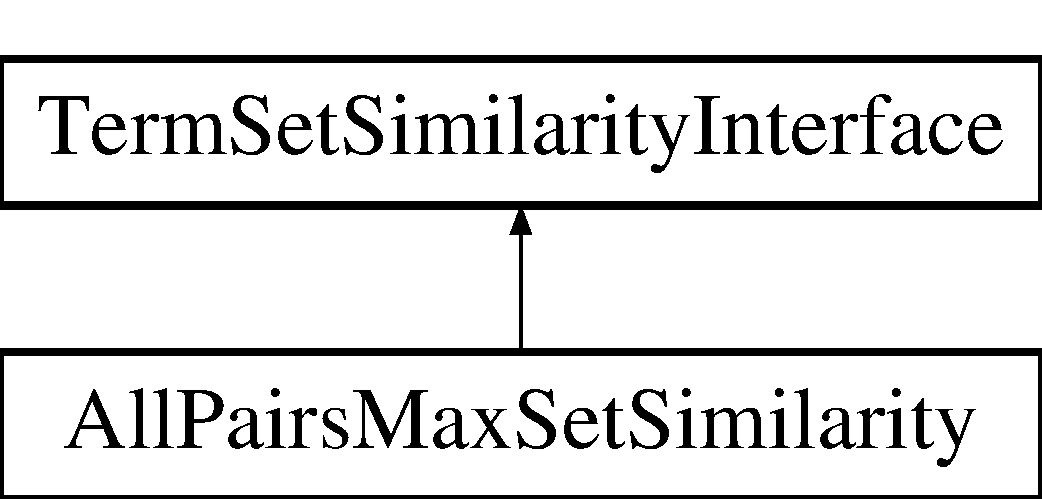
\includegraphics[height=2.000000cm]{classAllPairsMaxSetSimilarity}
\end{center}
\end{figure}
\subsection*{Public Member Functions}
\begin{DoxyCompactItemize}
\item 
\hyperlink{classAllPairsMaxSetSimilarity_a5aef6b55e2aa3b94b62278eb5464dd68}{All\+Pairs\+Max\+Set\+Similarity} (\hyperlink{classTermSimilarityInterface}{Term\+Similarity\+Interface} $\ast$sim\+Measure)
\begin{DoxyCompactList}\small\item\em Constructor. \end{DoxyCompactList}\item 
double \hyperlink{classAllPairsMaxSetSimilarity_a0eed3f63e2acdeb8365900b9d7a038c1}{calculate\+Similarity} (const boost\+::unordered\+\_\+set$<$ std\+::string $>$ \&termsA, const boost\+::unordered\+\_\+set$<$ std\+::string $>$ \&termsB)
\begin{DoxyCompactList}\small\item\em A method for calculating term set to term set similarity for \hyperlink{namespaceGO}{GO} terms;. \end{DoxyCompactList}\end{DoxyCompactItemize}


\subsection{Detailed Description}
A class to calculate the max similarity between all pairs of go terms for 2 sets. 

This class defines the all pairs max similarity between two sets of terms. Used by Sevilla et al.

J. L. Sevilla, V. Segura, A. Podhorski, E. Guruceaga, J. M. Mato, L. A. Martinez-\/\+Cruz, et al., \char`\"{}\+Correlation between gene expression and
 G\+O semantic similarity,\char`\"{} I\+E\+E\+E/\+A\+CM Trans Comput Biol Bioinform, vol. 2, pp. 330-\/8, Oct-\/\+Dec 2005. 

\subsection{Constructor \& Destructor Documentation}
\index{All\+Pairs\+Max\+Set\+Similarity@{All\+Pairs\+Max\+Set\+Similarity}!All\+Pairs\+Max\+Set\+Similarity@{All\+Pairs\+Max\+Set\+Similarity}}
\index{All\+Pairs\+Max\+Set\+Similarity@{All\+Pairs\+Max\+Set\+Similarity}!All\+Pairs\+Max\+Set\+Similarity@{All\+Pairs\+Max\+Set\+Similarity}}
\subsubsection[{\texorpdfstring{All\+Pairs\+Max\+Set\+Similarity(\+Term\+Similarity\+Interface $\ast$sim\+Measure)}{AllPairsMaxSetSimilarity(TermSimilarityInterface *simMeasure)}}]{\setlength{\rightskip}{0pt plus 5cm}All\+Pairs\+Max\+Set\+Similarity\+::\+All\+Pairs\+Max\+Set\+Similarity (
\begin{DoxyParamCaption}
\item[{{\bf Term\+Similarity\+Interface} $\ast$}]{sim\+Measure}
\end{DoxyParamCaption}
)\hspace{0.3cm}{\ttfamily [inline]}}\hypertarget{classAllPairsMaxSetSimilarity_a5aef6b55e2aa3b94b62278eb5464dd68}{}\label{classAllPairsMaxSetSimilarity_a5aef6b55e2aa3b94b62278eb5464dd68}


Constructor. 

Creates the \hyperlink{classAllPairsMaxSetSimilarity}{All\+Pairs\+Max\+Set\+Similarity} class assigning the similarity measure private memeber. 

\subsection{Member Function Documentation}
\index{All\+Pairs\+Max\+Set\+Similarity@{All\+Pairs\+Max\+Set\+Similarity}!calculate\+Similarity@{calculate\+Similarity}}
\index{calculate\+Similarity@{calculate\+Similarity}!All\+Pairs\+Max\+Set\+Similarity@{All\+Pairs\+Max\+Set\+Similarity}}
\subsubsection[{\texorpdfstring{calculate\+Similarity(const boost\+::unordered\+\_\+set$<$ std\+::string $>$ \&terms\+A, const boost\+::unordered\+\_\+set$<$ std\+::string $>$ \&terms\+B)}{calculateSimilarity(const boost::unordered_set< std::string > &termsA, const boost::unordered_set< std::string > &termsB)}}]{\setlength{\rightskip}{0pt plus 5cm}double All\+Pairs\+Max\+Set\+Similarity\+::calculate\+Similarity (
\begin{DoxyParamCaption}
\item[{const boost\+::unordered\+\_\+set$<$ std\+::string $>$ \&}]{termsA, }
\item[{const boost\+::unordered\+\_\+set$<$ std\+::string $>$ \&}]{termsB}
\end{DoxyParamCaption}
)\hspace{0.3cm}{\ttfamily [inline]}, {\ttfamily [virtual]}}\hypertarget{classAllPairsMaxSetSimilarity_a0eed3f63e2acdeb8365900b9d7a038c1}{}\label{classAllPairsMaxSetSimilarity_a0eed3f63e2acdeb8365900b9d7a038c1}


A method for calculating term set to term set similarity for \hyperlink{namespaceGO}{GO} terms;. 

This method returns the all pairs max similarity. 

Implements \hyperlink{classTermSetSimilarityInterface_aeb985b714efc3df40e55bdd31e425e04}{Term\+Set\+Similarity\+Interface}.



The documentation for this class was generated from the following file\+:\begin{DoxyCompactItemize}
\item 
ggtk/All\+Pairs\+Max\+Set\+Similarity.\+hpp\end{DoxyCompactItemize}

\hypertarget{classAncestorMeanSharedInformation}{}\section{Ancestor\+Mean\+Shared\+Information Class Reference}
\label{classAncestorMeanSharedInformation}\index{Ancestor\+Mean\+Shared\+Information@{Ancestor\+Mean\+Shared\+Information}}


A class to calculate shared infromation as the average information conent of all common ancestors.  




{\ttfamily \#include $<$ggtk/\+Ancestor\+Mean\+Shared\+Information.\+hpp$>$}

Inheritance diagram for Ancestor\+Mean\+Shared\+Information\+:\begin{figure}[H]
\begin{center}
\leavevmode
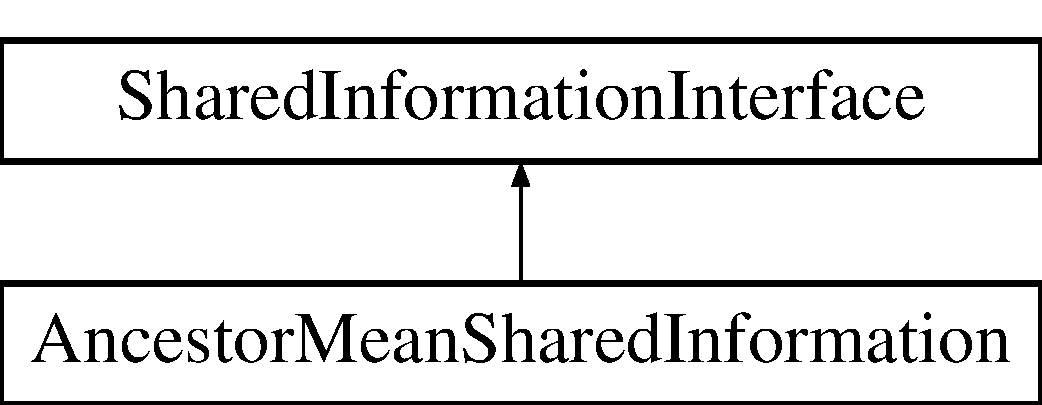
\includegraphics[height=2.000000cm]{classAncestorMeanSharedInformation}
\end{center}
\end{figure}
\subsection*{Public Member Functions}
\begin{DoxyCompactItemize}
\item 
\hyperlink{classAncestorMeanSharedInformation_aef781d2b6461b28b4974aa990611c8a1}{Ancestor\+Mean\+Shared\+Information} (\hyperlink{classGoGraph}{Go\+Graph} $\ast$go\+Graph, \hyperlink{classTermInformationContentMap}{Term\+Information\+Content\+Map} \&ic\+Map)
\begin{DoxyCompactList}\small\item\em A constructor. \end{DoxyCompactList}\item 
double \hyperlink{classAncestorMeanSharedInformation_a86dad7b02ff45ae758a2b311ad763350}{shared\+Information} (const std\+::string \&termA, const std\+::string \&termB)
\begin{DoxyCompactList}\small\item\em A method for calculating the shared infromation between two concepts. \end{DoxyCompactList}\item 
double \hyperlink{classAncestorMeanSharedInformation_af31937c58ee53db666586b446bc23061}{shared\+Information} (const std\+::string \&term)
\begin{DoxyCompactList}\small\item\em An interface method for returning the shared information of a single terms,or information content. \end{DoxyCompactList}\item 
double \hyperlink{classAncestorMeanSharedInformation_abf7d613e1459a5cf49071871e55f8a50}{max\+Information\+Content} (const std\+::string \&term)
\begin{DoxyCompactList}\small\item\em An interface method for returning the maximum information content for a term. \end{DoxyCompactList}\item 
bool \hyperlink{classAncestorMeanSharedInformation_af7503d6f761957bcb22d0e6614d87fa4}{has\+Term} (const std\+::string \&term)
\begin{DoxyCompactList}\small\item\em An interface method for determining if a term can be found. \end{DoxyCompactList}\item 
bool \hyperlink{classAncestorMeanSharedInformation_a75f59ac9d53014b967d0a81de8a07dbb}{is\+Same\+Ontology} (const std\+::string \&termA, const std\+::string \&termB)
\begin{DoxyCompactList}\small\item\em An interface method for determining if the two terms are of like ontologies. \end{DoxyCompactList}\end{DoxyCompactItemize}


\subsection{Detailed Description}
A class to calculate shared infromation as the average information conent of all common ancestors. 

This class calculates shared infromation by averaging the information content of all common ancestors.

This shared information method is used a baseline for comparison and may not be meaningful. 

\subsection{Constructor \& Destructor Documentation}
\index{Ancestor\+Mean\+Shared\+Information@{Ancestor\+Mean\+Shared\+Information}!Ancestor\+Mean\+Shared\+Information@{Ancestor\+Mean\+Shared\+Information}}
\index{Ancestor\+Mean\+Shared\+Information@{Ancestor\+Mean\+Shared\+Information}!Ancestor\+Mean\+Shared\+Information@{Ancestor\+Mean\+Shared\+Information}}
\subsubsection[{\texorpdfstring{Ancestor\+Mean\+Shared\+Information(\+Go\+Graph $\ast$go\+Graph, Term\+Information\+Content\+Map \&ic\+Map)}{AncestorMeanSharedInformation(GoGraph *goGraph, TermInformationContentMap &icMap)}}]{\setlength{\rightskip}{0pt plus 5cm}Ancestor\+Mean\+Shared\+Information\+::\+Ancestor\+Mean\+Shared\+Information (
\begin{DoxyParamCaption}
\item[{{\bf Go\+Graph} $\ast$}]{go\+Graph, }
\item[{{\bf Term\+Information\+Content\+Map} \&}]{ic\+Map}
\end{DoxyParamCaption}
)\hspace{0.3cm}{\ttfamily [inline]}}\hypertarget{classAncestorMeanSharedInformation_aef781d2b6461b28b4974aa990611c8a1}{}\label{classAncestorMeanSharedInformation_aef781d2b6461b28b4974aa990611c8a1}


A constructor. 

Creates the \hyperlink{classAncestorMeanSharedInformation}{Ancestor\+Mean\+Shared\+Information} class 

\subsection{Member Function Documentation}
\index{Ancestor\+Mean\+Shared\+Information@{Ancestor\+Mean\+Shared\+Information}!has\+Term@{has\+Term}}
\index{has\+Term@{has\+Term}!Ancestor\+Mean\+Shared\+Information@{Ancestor\+Mean\+Shared\+Information}}
\subsubsection[{\texorpdfstring{has\+Term(const std\+::string \&term)}{hasTerm(const std::string &term)}}]{\setlength{\rightskip}{0pt plus 5cm}bool Ancestor\+Mean\+Shared\+Information\+::has\+Term (
\begin{DoxyParamCaption}
\item[{const std\+::string \&}]{term}
\end{DoxyParamCaption}
)\hspace{0.3cm}{\ttfamily [inline]}, {\ttfamily [virtual]}}\hypertarget{classAncestorMeanSharedInformation_af7503d6f761957bcb22d0e6614d87fa4}{}\label{classAncestorMeanSharedInformation_af7503d6f761957bcb22d0e6614d87fa4}


An interface method for determining if a term can be found. 

Determines if the term can be found in the current map. 

Implements \hyperlink{classSharedInformationInterface_a3f056cf6a40eea8c1669108087dcd5c8}{Shared\+Information\+Interface}.

\index{Ancestor\+Mean\+Shared\+Information@{Ancestor\+Mean\+Shared\+Information}!is\+Same\+Ontology@{is\+Same\+Ontology}}
\index{is\+Same\+Ontology@{is\+Same\+Ontology}!Ancestor\+Mean\+Shared\+Information@{Ancestor\+Mean\+Shared\+Information}}
\subsubsection[{\texorpdfstring{is\+Same\+Ontology(const std\+::string \&term\+A, const std\+::string \&term\+B)}{isSameOntology(const std::string &termA, const std::string &termB)}}]{\setlength{\rightskip}{0pt plus 5cm}bool Ancestor\+Mean\+Shared\+Information\+::is\+Same\+Ontology (
\begin{DoxyParamCaption}
\item[{const std\+::string \&}]{termA, }
\item[{const std\+::string \&}]{termB}
\end{DoxyParamCaption}
)\hspace{0.3cm}{\ttfamily [inline]}, {\ttfamily [virtual]}}\hypertarget{classAncestorMeanSharedInformation_a75f59ac9d53014b967d0a81de8a07dbb}{}\label{classAncestorMeanSharedInformation_a75f59ac9d53014b967d0a81de8a07dbb}


An interface method for determining if the two terms are of like ontologies. 

Determine if two terms are of the same ontology. 

Implements \hyperlink{classSharedInformationInterface_a607463b9736df9c4b8ec3ba9fe41c19d}{Shared\+Information\+Interface}.

\index{Ancestor\+Mean\+Shared\+Information@{Ancestor\+Mean\+Shared\+Information}!max\+Information\+Content@{max\+Information\+Content}}
\index{max\+Information\+Content@{max\+Information\+Content}!Ancestor\+Mean\+Shared\+Information@{Ancestor\+Mean\+Shared\+Information}}
\subsubsection[{\texorpdfstring{max\+Information\+Content(const std\+::string \&term)}{maxInformationContent(const std::string &term)}}]{\setlength{\rightskip}{0pt plus 5cm}double Ancestor\+Mean\+Shared\+Information\+::max\+Information\+Content (
\begin{DoxyParamCaption}
\item[{const std\+::string \&}]{term}
\end{DoxyParamCaption}
)\hspace{0.3cm}{\ttfamily [inline]}, {\ttfamily [virtual]}}\hypertarget{classAncestorMeanSharedInformation_abf7d613e1459a5cf49071871e55f8a50}{}\label{classAncestorMeanSharedInformation_abf7d613e1459a5cf49071871e55f8a50}


An interface method for returning the maximum information content for a term. 

This method provides the absolute max information content within a corpus for normalization purposes. 

Implements \hyperlink{classSharedInformationInterface_a7356ba99509458777972ce0f00ebd999}{Shared\+Information\+Interface}.

\index{Ancestor\+Mean\+Shared\+Information@{Ancestor\+Mean\+Shared\+Information}!shared\+Information@{shared\+Information}}
\index{shared\+Information@{shared\+Information}!Ancestor\+Mean\+Shared\+Information@{Ancestor\+Mean\+Shared\+Information}}
\subsubsection[{\texorpdfstring{shared\+Information(const std\+::string \&term\+A, const std\+::string \&term\+B)}{sharedInformation(const std::string &termA, const std::string &termB)}}]{\setlength{\rightskip}{0pt plus 5cm}double Ancestor\+Mean\+Shared\+Information\+::shared\+Information (
\begin{DoxyParamCaption}
\item[{const std\+::string \&}]{termA, }
\item[{const std\+::string \&}]{termB}
\end{DoxyParamCaption}
)\hspace{0.3cm}{\ttfamily [inline]}, {\ttfamily [virtual]}}\hypertarget{classAncestorMeanSharedInformation_a86dad7b02ff45ae758a2b311ad763350}{}\label{classAncestorMeanSharedInformation_a86dad7b02ff45ae758a2b311ad763350}


A method for calculating the shared infromation between two concepts. 

This method returns the shared information between two concepts. 

Implements \hyperlink{classSharedInformationInterface_a76e8858eb598442b86b0fd3be1c519e7}{Shared\+Information\+Interface}.

\index{Ancestor\+Mean\+Shared\+Information@{Ancestor\+Mean\+Shared\+Information}!shared\+Information@{shared\+Information}}
\index{shared\+Information@{shared\+Information}!Ancestor\+Mean\+Shared\+Information@{Ancestor\+Mean\+Shared\+Information}}
\subsubsection[{\texorpdfstring{shared\+Information(const std\+::string \&term)}{sharedInformation(const std::string &term)}}]{\setlength{\rightskip}{0pt plus 5cm}double Ancestor\+Mean\+Shared\+Information\+::shared\+Information (
\begin{DoxyParamCaption}
\item[{const std\+::string \&}]{term}
\end{DoxyParamCaption}
)\hspace{0.3cm}{\ttfamily [inline]}, {\ttfamily [virtual]}}\hypertarget{classAncestorMeanSharedInformation_af31937c58ee53db666586b446bc23061}{}\label{classAncestorMeanSharedInformation_af31937c58ee53db666586b446bc23061}


An interface method for returning the shared information of a single terms,or information content. 

This method privdes a mechanism for returing a term\textquotesingle{}s infromation content. 

Implements \hyperlink{classSharedInformationInterface_aba102c0e44fbc098baef6074f1eb37b6}{Shared\+Information\+Interface}.



The documentation for this class was generated from the following file\+:\begin{DoxyCompactItemize}
\item 
ggtk/Ancestor\+Mean\+Shared\+Information.\+hpp\end{DoxyCompactItemize}

\hypertarget{classAnnotationData}{}\section{Annotation\+Data Class Reference}
\label{classAnnotationData}\index{Annotation\+Data@{Annotation\+Data}}


A class for storing information about genes annotated with go terms.  




{\ttfamily \#include $<$ggtk/\+Annotation\+Data.\+hpp$>$}

\subsection*{Public Member Functions}
\begin{DoxyCompactItemize}
\item 
\hyperlink{classAnnotationData_aa72d292d4f480d2e580ba4d39b88ab8f}{Annotation\+Data} ()
\begin{DoxyCompactList}\small\item\em Class constructor. \end{DoxyCompactList}\item 
\hyperlink{classAnnotationData_a3abda2766658360884f8097cf4ea5281}{$\sim$\+Annotation\+Data} ()
\begin{DoxyCompactList}\small\item\em class descructor \end{DoxyCompactList}\item 
void \hyperlink{classAnnotationData_ac6bd9048c83a52ebaa9a9e83a45e7f4a}{add\+Association} (const std\+::string \&gene, const std\+::string \&go\+Term, const std\+::string \&evidence\+Code)
\begin{DoxyCompactList}\small\item\em A Method to add annotations to the dataset. \end{DoxyCompactList}\item 
bool \hyperlink{classAnnotationData_a406a75a2f26bb7597f27599daf5416ad}{has\+Go\+Term} (const std\+::string \&go\+Term)
\begin{DoxyCompactList}\small\item\em This method tests the existence of a term in the database. \end{DoxyCompactList}\item 
bool \hyperlink{classAnnotationData_af1456f7623ce06262d8782a01fd2ca9c}{has\+Gene} (const std\+::string \&gene)
\begin{DoxyCompactList}\small\item\em This method tests the existence of a gene in the database. \end{DoxyCompactList}\item 
std\+::vector$<$ std\+::string $>$ \hyperlink{classAnnotationData_a8b99d05f5f0f619958e7850253946b9c}{get\+All\+Go\+Terms} ()
\begin{DoxyCompactList}\small\item\em This method returns all the go terms in the database. \end{DoxyCompactList}\item 
std\+::vector$<$ std\+::string $>$ \hyperlink{classAnnotationData_aa2d7d5ad9601b6984470b8267ff37db8}{get\+All\+Genes} ()
\begin{DoxyCompactList}\small\item\em This method returns all genes in the database. \end{DoxyCompactList}\item 
std\+::vector$<$ std\+::string $>$ \hyperlink{classAnnotationData_aee62a418cae2da15f4b3a4bd9f933376}{get\+Go\+Terms\+For\+Gene} (const std\+::string \&gene)
\begin{DoxyCompactList}\small\item\em This method gets the go terms for a gene. \end{DoxyCompactList}\item 
boost\+::unordered\+\_\+set$<$ std\+::string $>$ \hyperlink{classAnnotationData_ad1864b7768ab74d74be296e546269881}{get\+Go\+Terms\+For\+Gene\+By\+Ontology} (const std\+::string \&gene, \hyperlink{namespaceGO_a5ae335887b5cf40a9ef3045be9247fc3}{G\+O\+::\+Onto} filter\+Ontology, \hyperlink{classGoGraph}{Go\+Graph} $\ast$G)
\begin{DoxyCompactList}\small\item\em This method gets the go terms for a gene within the specified onotlogy. \end{DoxyCompactList}\item 
boost\+::unordered\+\_\+set$<$ std\+::string $>$ \hyperlink{classAnnotationData_a86fa8eaf6310627d530ab118c6e1e22b}{get\+Go\+Terms\+For\+Gene\+BP} (const std\+::string \&gene, \hyperlink{classGoGraph}{Go\+Graph} $\ast$G)
\begin{DoxyCompactList}\small\item\em This method gets the biological process go terms for a gene. \end{DoxyCompactList}\item 
boost\+::unordered\+\_\+set$<$ std\+::string $>$ \hyperlink{classAnnotationData_ab9639d4828270517550a3e739d03317b}{get\+Go\+Terms\+For\+Gene\+MF} (const std\+::string \&gene, \hyperlink{classGoGraph}{Go\+Graph} $\ast$G)
\begin{DoxyCompactList}\small\item\em This method gets the molecular function go terms for a gene. \end{DoxyCompactList}\item 
boost\+::unordered\+\_\+set$<$ std\+::string $>$ \hyperlink{classAnnotationData_a37679ed0830c6d7ec41672b3df541663}{get\+Go\+Terms\+For\+Gene\+CC} (const std\+::string \&gene, \hyperlink{classGoGraph}{Go\+Graph} $\ast$G)
\begin{DoxyCompactList}\small\item\em This method gets the cellular component go terms for a gene. \end{DoxyCompactList}\item 
std\+::vector$<$ std\+::string $>$ \hyperlink{classAnnotationData_a4f61ca3276af902c72a031419e8155c5}{get\+Go\+Terms\+Evidence\+For\+Gene} (const std\+::string \&gene)
\begin{DoxyCompactList}\small\item\em A method to get the evidence codes for a list of go terms. \end{DoxyCompactList}\item 
std\+::vector$<$ std\+::string $>$ \hyperlink{classAnnotationData_a0028d38de841c5a508ad602907b42be7}{get\+Genes\+For\+Go\+Term} (const std\+::string \&go\+Term)
\begin{DoxyCompactList}\small\item\em This method gets the genes for a go term. \end{DoxyCompactList}\item 
void \hyperlink{classAnnotationData_adcae89b874856e2e30319382a51f3c14}{add\+Genes\+For\+Go\+Term} (const std\+::string \&go\+Term, boost\+::unordered\+\_\+set$<$ std\+::string $>$ \&gene\+Set)
\begin{DoxyCompactList}\small\item\em This method adds the genes for a go term to a set. \end{DoxyCompactList}\item 
std\+::vector$<$ std\+::string $>$ \hyperlink{classAnnotationData_a95cf54dc33c9f4e948e913424a44c52e}{get\+Genes\+Evidence\+For\+Go\+Term} (const std\+::string \&go\+Term)
\begin{DoxyCompactList}\small\item\em A method to get the evidence codes for a list of genes. \end{DoxyCompactList}\item 
std\+::size\+\_\+t \hyperlink{classAnnotationData_a985193a995893976a17f09217cced074}{get\+Num\+Annotations\+For\+Go\+Term} (const std\+::string \&go\+Term)
\begin{DoxyCompactList}\small\item\em A method to get the number of annotations of a particular go term. \end{DoxyCompactList}\item 
std\+::size\+\_\+t \hyperlink{classAnnotationData_a367c90051704e541d674d1ee222e6bbe}{get\+Num\+Annotations\+For\+Gene} (const std\+::string \&gene)
\begin{DoxyCompactList}\small\item\em A method to get the number of annotations of a particular gene. \end{DoxyCompactList}\item 
std\+::size\+\_\+t \hyperlink{classAnnotationData_aa3eeff87e44cc21e06cc5f49899cf776}{get\+Num\+Genes} ()
\begin{DoxyCompactList}\small\item\em A helper method to get the number of genes in the db. \end{DoxyCompactList}\item 
std\+::size\+\_\+t \hyperlink{classAnnotationData_ad47dc3da1210218c0bb90ca80f6355ec}{get\+Num\+Go\+Terms} ()
\begin{DoxyCompactList}\small\item\em A helper method to get the number of go terms in the db. \end{DoxyCompactList}\item 
std\+::vector$<$ std\+::string $>$ \hyperlink{classAnnotationData_a25a5ccfa938a1d623e8f162f2959d951}{get\+Ontology\+Terms} (\hyperlink{classGoGraph}{Go\+Graph} $\ast$graph, \hyperlink{namespaceGO_a5ae335887b5cf40a9ef3045be9247fc3}{G\+O\+::\+Onto} ontology)
\begin{DoxyCompactList}\small\item\em A helper method to return only the terms of the give ontology. \end{DoxyCompactList}\end{DoxyCompactItemize}
\subsection*{Public Attributes}
\begin{DoxyCompactItemize}
\item 
std\+::vector$<$ std\+::string $>$ \hyperlink{classAnnotationData_a9f25041cb6cfabe964e2857b54400a3b}{\+\_\+genes}
\begin{DoxyCompactList}\small\item\em A list of genes stored by the annotation data object. \end{DoxyCompactList}\item 
std\+::vector$<$ std\+::string $>$ \hyperlink{classAnnotationData_a88170d72e7addb555701e7aeba30f588}{\+\_\+go\+Terms}
\begin{DoxyCompactList}\small\item\em A list of go terms stored by the annotation data object. \end{DoxyCompactList}\item 
boost\+::unordered\+\_\+map$<$ std\+::string, std\+::size\+\_\+t $>$ \hyperlink{classAnnotationData_a2246453b69594c15745d47f6c3c4c533}{\+\_\+string\+To\+Gene}
\begin{DoxyCompactList}\small\item\em A map from a gene strings to a gene index. \end{DoxyCompactList}\item 
boost\+::unordered\+\_\+map$<$ std\+::string, std\+::size\+\_\+t $>$ \hyperlink{classAnnotationData_ab743686bf79303fbc0eb16c323d1b104}{\+\_\+string\+To\+Go}
\begin{DoxyCompactList}\small\item\em A map from a go term strings to a go term index. \end{DoxyCompactList}\item 
std\+::vector$<$ std\+::vector$<$ std\+::size\+\_\+t $>$ $>$ \hyperlink{classAnnotationData_a72a19fdf14001e241bd0dc200c5fd0de}{\+\_\+go\+To\+Genes}
\begin{DoxyCompactList}\small\item\em A list of lists of genes, one for each go term. \end{DoxyCompactList}\item 
std\+::vector$<$ std\+::vector$<$ \hyperlink{namespaceGO_a4ce5387bbcdaec3648957c7903f2caf3}{G\+O\+::\+Evidence\+Code} $>$ $>$ \hyperlink{classAnnotationData_afdad9a39d18deaf76fae099554caf86e}{\+\_\+go\+To\+Genes\+Evidence}
\begin{DoxyCompactList}\small\item\em A list of lists of evidence codes, one for each go term. Parallel to \+\_\+go\+To\+Genes. \end{DoxyCompactList}\item 
std\+::vector$<$ std\+::vector$<$ std\+::size\+\_\+t $>$ $>$ \hyperlink{classAnnotationData_aa936d0cc30ba41aa177c5fd0867f38db}{\+\_\+gene\+To\+Gos}
\begin{DoxyCompactList}\small\item\em A list of lists of go terms, one for each gene. \end{DoxyCompactList}\item 
std\+::vector$<$ std\+::vector$<$ \hyperlink{namespaceGO_a4ce5387bbcdaec3648957c7903f2caf3}{G\+O\+::\+Evidence\+Code} $>$ $>$ \hyperlink{classAnnotationData_a6bf6ba78c786caf078731b87357f96c0}{\+\_\+gene\+To\+Gos\+Evidence}
\begin{DoxyCompactList}\small\item\em A list of lists of evidence codes, one for each gene. Parallel to \+\_\+gene\+To\+Gos. \end{DoxyCompactList}\end{DoxyCompactItemize}


\subsection{Detailed Description}
A class for storing information about genes annotated with go terms. 

This class hold all information about a set of annotations for genes annotated with go terms. It holds a list of genes, a list of go terms, as well as mappings from a gene to a list of go terms, and mappings from a go term to a list of annotated genes. This class allows querying go annotations and their evidence codes. 

\subsection{Constructor \& Destructor Documentation}
\index{Annotation\+Data@{Annotation\+Data}!Annotation\+Data@{Annotation\+Data}}
\index{Annotation\+Data@{Annotation\+Data}!Annotation\+Data@{Annotation\+Data}}
\subsubsection[{\texorpdfstring{Annotation\+Data()}{AnnotationData()}}]{\setlength{\rightskip}{0pt plus 5cm}Annotation\+Data\+::\+Annotation\+Data (
\begin{DoxyParamCaption}
{}
\end{DoxyParamCaption}
)\hspace{0.3cm}{\ttfamily [inline]}}\hypertarget{classAnnotationData_aa72d292d4f480d2e580ba4d39b88ab8f}{}\label{classAnnotationData_aa72d292d4f480d2e580ba4d39b88ab8f}


Class constructor. 

This constructor initialized each vector as an empty vector of the correct type. \index{Annotation\+Data@{Annotation\+Data}!````~Annotation\+Data@{$\sim$\+Annotation\+Data}}
\index{````~Annotation\+Data@{$\sim$\+Annotation\+Data}!Annotation\+Data@{Annotation\+Data}}
\subsubsection[{\texorpdfstring{$\sim$\+Annotation\+Data()}{~AnnotationData()}}]{\setlength{\rightskip}{0pt plus 5cm}Annotation\+Data\+::$\sim$\+Annotation\+Data (
\begin{DoxyParamCaption}
{}
\end{DoxyParamCaption}
)\hspace{0.3cm}{\ttfamily [inline]}}\hypertarget{classAnnotationData_a3abda2766658360884f8097cf4ea5281}{}\label{classAnnotationData_a3abda2766658360884f8097cf4ea5281}


class descructor 

This destructor clears all maps and vectors. 

\subsection{Member Function Documentation}
\index{Annotation\+Data@{Annotation\+Data}!add\+Association@{add\+Association}}
\index{add\+Association@{add\+Association}!Annotation\+Data@{Annotation\+Data}}
\subsubsection[{\texorpdfstring{add\+Association(const std\+::string \&gene, const std\+::string \&go\+Term, const std\+::string \&evidence\+Code)}{addAssociation(const std::string &gene, const std::string &goTerm, const std::string &evidenceCode)}}]{\setlength{\rightskip}{0pt plus 5cm}void Annotation\+Data\+::add\+Association (
\begin{DoxyParamCaption}
\item[{const std\+::string \&}]{gene, }
\item[{const std\+::string \&}]{go\+Term, }
\item[{const std\+::string \&}]{evidence\+Code}
\end{DoxyParamCaption}
)\hspace{0.3cm}{\ttfamily [inline]}}\hypertarget{classAnnotationData_ac6bd9048c83a52ebaa9a9e83a45e7f4a}{}\label{classAnnotationData_ac6bd9048c83a52ebaa9a9e83a45e7f4a}


A Method to add annotations to the dataset. 

This method adds annotations to the database. It takes a gene, a go\+Term, and an evidence code. This method checks existence and indexing to remove the burden from parser implementations. \index{Annotation\+Data@{Annotation\+Data}!add\+Genes\+For\+Go\+Term@{add\+Genes\+For\+Go\+Term}}
\index{add\+Genes\+For\+Go\+Term@{add\+Genes\+For\+Go\+Term}!Annotation\+Data@{Annotation\+Data}}
\subsubsection[{\texorpdfstring{add\+Genes\+For\+Go\+Term(const std\+::string \&go\+Term, boost\+::unordered\+\_\+set$<$ std\+::string $>$ \&gene\+Set)}{addGenesForGoTerm(const std::string &goTerm, boost::unordered_set< std::string > &geneSet)}}]{\setlength{\rightskip}{0pt plus 5cm}void Annotation\+Data\+::add\+Genes\+For\+Go\+Term (
\begin{DoxyParamCaption}
\item[{const std\+::string \&}]{go\+Term, }
\item[{boost\+::unordered\+\_\+set$<$ std\+::string $>$ \&}]{gene\+Set}
\end{DoxyParamCaption}
)\hspace{0.3cm}{\ttfamily [inline]}}\hypertarget{classAnnotationData_adcae89b874856e2e30319382a51f3c14}{}\label{classAnnotationData_adcae89b874856e2e30319382a51f3c14}


This method adds the genes for a go term to a set. 

A helper method to add genes associated to a term to a set of genes. Used in enrichment calculation \index{Annotation\+Data@{Annotation\+Data}!get\+All\+Genes@{get\+All\+Genes}}
\index{get\+All\+Genes@{get\+All\+Genes}!Annotation\+Data@{Annotation\+Data}}
\subsubsection[{\texorpdfstring{get\+All\+Genes()}{getAllGenes()}}]{\setlength{\rightskip}{0pt plus 5cm}std\+::vector$<$std\+::string$>$ Annotation\+Data\+::get\+All\+Genes (
\begin{DoxyParamCaption}
{}
\end{DoxyParamCaption}
)\hspace{0.3cm}{\ttfamily [inline]}}\hypertarget{classAnnotationData_aa2d7d5ad9601b6984470b8267ff37db8}{}\label{classAnnotationData_aa2d7d5ad9601b6984470b8267ff37db8}


This method returns all genes in the database. 

A helper method to return all the genes in the databse \index{Annotation\+Data@{Annotation\+Data}!get\+All\+Go\+Terms@{get\+All\+Go\+Terms}}
\index{get\+All\+Go\+Terms@{get\+All\+Go\+Terms}!Annotation\+Data@{Annotation\+Data}}
\subsubsection[{\texorpdfstring{get\+All\+Go\+Terms()}{getAllGoTerms()}}]{\setlength{\rightskip}{0pt plus 5cm}std\+::vector$<$std\+::string$>$ Annotation\+Data\+::get\+All\+Go\+Terms (
\begin{DoxyParamCaption}
{}
\end{DoxyParamCaption}
)\hspace{0.3cm}{\ttfamily [inline]}}\hypertarget{classAnnotationData_a8b99d05f5f0f619958e7850253946b9c}{}\label{classAnnotationData_a8b99d05f5f0f619958e7850253946b9c}


This method returns all the go terms in the database. 

A helper method to return all the \hyperlink{namespaceGO}{GO} terms in the databse \index{Annotation\+Data@{Annotation\+Data}!get\+Genes\+Evidence\+For\+Go\+Term@{get\+Genes\+Evidence\+For\+Go\+Term}}
\index{get\+Genes\+Evidence\+For\+Go\+Term@{get\+Genes\+Evidence\+For\+Go\+Term}!Annotation\+Data@{Annotation\+Data}}
\subsubsection[{\texorpdfstring{get\+Genes\+Evidence\+For\+Go\+Term(const std\+::string \&go\+Term)}{getGenesEvidenceForGoTerm(const std::string &goTerm)}}]{\setlength{\rightskip}{0pt plus 5cm}std\+::vector$<$std\+::string$>$ Annotation\+Data\+::get\+Genes\+Evidence\+For\+Go\+Term (
\begin{DoxyParamCaption}
\item[{const std\+::string \&}]{go\+Term}
\end{DoxyParamCaption}
)\hspace{0.3cm}{\ttfamily [inline]}}\hypertarget{classAnnotationData_a95cf54dc33c9f4e948e913424a44c52e}{}\label{classAnnotationData_a95cf54dc33c9f4e948e913424a44c52e}


A method to get the evidence codes for a list of genes. 

This method returns the evidence codes for a list of genes. It parallels the get\+Genes\+For\+Go\+Term method and is used for printing and testing. \index{Annotation\+Data@{Annotation\+Data}!get\+Genes\+For\+Go\+Term@{get\+Genes\+For\+Go\+Term}}
\index{get\+Genes\+For\+Go\+Term@{get\+Genes\+For\+Go\+Term}!Annotation\+Data@{Annotation\+Data}}
\subsubsection[{\texorpdfstring{get\+Genes\+For\+Go\+Term(const std\+::string \&go\+Term)}{getGenesForGoTerm(const std::string &goTerm)}}]{\setlength{\rightskip}{0pt plus 5cm}std\+::vector$<$std\+::string$>$ Annotation\+Data\+::get\+Genes\+For\+Go\+Term (
\begin{DoxyParamCaption}
\item[{const std\+::string \&}]{go\+Term}
\end{DoxyParamCaption}
)\hspace{0.3cm}{\ttfamily [inline]}}\hypertarget{classAnnotationData_a0028d38de841c5a508ad602907b42be7}{}\label{classAnnotationData_a0028d38de841c5a508ad602907b42be7}


This method gets the genes for a go term. 

A helper method to return, for a go term, a list of genes as a vector of strings. \index{Annotation\+Data@{Annotation\+Data}!get\+Go\+Terms\+Evidence\+For\+Gene@{get\+Go\+Terms\+Evidence\+For\+Gene}}
\index{get\+Go\+Terms\+Evidence\+For\+Gene@{get\+Go\+Terms\+Evidence\+For\+Gene}!Annotation\+Data@{Annotation\+Data}}
\subsubsection[{\texorpdfstring{get\+Go\+Terms\+Evidence\+For\+Gene(const std\+::string \&gene)}{getGoTermsEvidenceForGene(const std::string &gene)}}]{\setlength{\rightskip}{0pt plus 5cm}std\+::vector$<$std\+::string$>$ Annotation\+Data\+::get\+Go\+Terms\+Evidence\+For\+Gene (
\begin{DoxyParamCaption}
\item[{const std\+::string \&}]{gene}
\end{DoxyParamCaption}
)\hspace{0.3cm}{\ttfamily [inline]}}\hypertarget{classAnnotationData_a4f61ca3276af902c72a031419e8155c5}{}\label{classAnnotationData_a4f61ca3276af902c72a031419e8155c5}


A method to get the evidence codes for a list of go terms. 

This method returns the evidence codes for a list of go terms. It parallels the get\+Go\+Terms\+For\+Gene method and is used for printing and testing. \index{Annotation\+Data@{Annotation\+Data}!get\+Go\+Terms\+For\+Gene@{get\+Go\+Terms\+For\+Gene}}
\index{get\+Go\+Terms\+For\+Gene@{get\+Go\+Terms\+For\+Gene}!Annotation\+Data@{Annotation\+Data}}
\subsubsection[{\texorpdfstring{get\+Go\+Terms\+For\+Gene(const std\+::string \&gene)}{getGoTermsForGene(const std::string &gene)}}]{\setlength{\rightskip}{0pt plus 5cm}std\+::vector$<$std\+::string$>$ Annotation\+Data\+::get\+Go\+Terms\+For\+Gene (
\begin{DoxyParamCaption}
\item[{const std\+::string \&}]{gene}
\end{DoxyParamCaption}
)\hspace{0.3cm}{\ttfamily [inline]}}\hypertarget{classAnnotationData_aee62a418cae2da15f4b3a4bd9f933376}{}\label{classAnnotationData_aee62a418cae2da15f4b3a4bd9f933376}


This method gets the go terms for a gene. 

A helper method to return, for a gene, a list of go terms as a vector of strings. \index{Annotation\+Data@{Annotation\+Data}!get\+Go\+Terms\+For\+Gene\+BP@{get\+Go\+Terms\+For\+Gene\+BP}}
\index{get\+Go\+Terms\+For\+Gene\+BP@{get\+Go\+Terms\+For\+Gene\+BP}!Annotation\+Data@{Annotation\+Data}}
\subsubsection[{\texorpdfstring{get\+Go\+Terms\+For\+Gene\+B\+P(const std\+::string \&gene, Go\+Graph $\ast$\+G)}{getGoTermsForGeneBP(const std::string &gene, GoGraph *G)}}]{\setlength{\rightskip}{0pt plus 5cm}boost\+::unordered\+\_\+set$<$std\+::string$>$ Annotation\+Data\+::get\+Go\+Terms\+For\+Gene\+BP (
\begin{DoxyParamCaption}
\item[{const std\+::string \&}]{gene, }
\item[{{\bf Go\+Graph} $\ast$}]{G}
\end{DoxyParamCaption}
)\hspace{0.3cm}{\ttfamily [inline]}}\hypertarget{classAnnotationData_a86fa8eaf6310627d530ab118c6e1e22b}{}\label{classAnnotationData_a86fa8eaf6310627d530ab118c6e1e22b}


This method gets the biological process go terms for a gene. 

A helper method to return a list of BP go terms for a gene. \index{Annotation\+Data@{Annotation\+Data}!get\+Go\+Terms\+For\+Gene\+By\+Ontology@{get\+Go\+Terms\+For\+Gene\+By\+Ontology}}
\index{get\+Go\+Terms\+For\+Gene\+By\+Ontology@{get\+Go\+Terms\+For\+Gene\+By\+Ontology}!Annotation\+Data@{Annotation\+Data}}
\subsubsection[{\texorpdfstring{get\+Go\+Terms\+For\+Gene\+By\+Ontology(const std\+::string \&gene, G\+O\+::\+Onto filter\+Ontology, Go\+Graph $\ast$\+G)}{getGoTermsForGeneByOntology(const std::string &gene, GO::Onto filterOntology, GoGraph *G)}}]{\setlength{\rightskip}{0pt plus 5cm}boost\+::unordered\+\_\+set$<$std\+::string$>$ Annotation\+Data\+::get\+Go\+Terms\+For\+Gene\+By\+Ontology (
\begin{DoxyParamCaption}
\item[{const std\+::string \&}]{gene, }
\item[{{\bf G\+O\+::\+Onto}}]{filter\+Ontology, }
\item[{{\bf Go\+Graph} $\ast$}]{G}
\end{DoxyParamCaption}
)\hspace{0.3cm}{\ttfamily [inline]}}\hypertarget{classAnnotationData_ad1864b7768ab74d74be296e546269881}{}\label{classAnnotationData_ad1864b7768ab74d74be296e546269881}


This method gets the go terms for a gene within the specified onotlogy. 

A helper method to return a list of go terms as a set of strings for a gene given the sub ontology BP, MF, or CC. \index{Annotation\+Data@{Annotation\+Data}!get\+Go\+Terms\+For\+Gene\+CC@{get\+Go\+Terms\+For\+Gene\+CC}}
\index{get\+Go\+Terms\+For\+Gene\+CC@{get\+Go\+Terms\+For\+Gene\+CC}!Annotation\+Data@{Annotation\+Data}}
\subsubsection[{\texorpdfstring{get\+Go\+Terms\+For\+Gene\+C\+C(const std\+::string \&gene, Go\+Graph $\ast$\+G)}{getGoTermsForGeneCC(const std::string &gene, GoGraph *G)}}]{\setlength{\rightskip}{0pt plus 5cm}boost\+::unordered\+\_\+set$<$std\+::string$>$ Annotation\+Data\+::get\+Go\+Terms\+For\+Gene\+CC (
\begin{DoxyParamCaption}
\item[{const std\+::string \&}]{gene, }
\item[{{\bf Go\+Graph} $\ast$}]{G}
\end{DoxyParamCaption}
)\hspace{0.3cm}{\ttfamily [inline]}}\hypertarget{classAnnotationData_a37679ed0830c6d7ec41672b3df541663}{}\label{classAnnotationData_a37679ed0830c6d7ec41672b3df541663}


This method gets the cellular component go terms for a gene. 

A helper method to return a list of CC go terms for a gene. \index{Annotation\+Data@{Annotation\+Data}!get\+Go\+Terms\+For\+Gene\+MF@{get\+Go\+Terms\+For\+Gene\+MF}}
\index{get\+Go\+Terms\+For\+Gene\+MF@{get\+Go\+Terms\+For\+Gene\+MF}!Annotation\+Data@{Annotation\+Data}}
\subsubsection[{\texorpdfstring{get\+Go\+Terms\+For\+Gene\+M\+F(const std\+::string \&gene, Go\+Graph $\ast$\+G)}{getGoTermsForGeneMF(const std::string &gene, GoGraph *G)}}]{\setlength{\rightskip}{0pt plus 5cm}boost\+::unordered\+\_\+set$<$std\+::string$>$ Annotation\+Data\+::get\+Go\+Terms\+For\+Gene\+MF (
\begin{DoxyParamCaption}
\item[{const std\+::string \&}]{gene, }
\item[{{\bf Go\+Graph} $\ast$}]{G}
\end{DoxyParamCaption}
)\hspace{0.3cm}{\ttfamily [inline]}}\hypertarget{classAnnotationData_ab9639d4828270517550a3e739d03317b}{}\label{classAnnotationData_ab9639d4828270517550a3e739d03317b}


This method gets the molecular function go terms for a gene. 

A helper method to return a list of MF go terms for a gene. \index{Annotation\+Data@{Annotation\+Data}!get\+Num\+Annotations\+For\+Gene@{get\+Num\+Annotations\+For\+Gene}}
\index{get\+Num\+Annotations\+For\+Gene@{get\+Num\+Annotations\+For\+Gene}!Annotation\+Data@{Annotation\+Data}}
\subsubsection[{\texorpdfstring{get\+Num\+Annotations\+For\+Gene(const std\+::string \&gene)}{getNumAnnotationsForGene(const std::string &gene)}}]{\setlength{\rightskip}{0pt plus 5cm}std\+::size\+\_\+t Annotation\+Data\+::get\+Num\+Annotations\+For\+Gene (
\begin{DoxyParamCaption}
\item[{const std\+::string \&}]{gene}
\end{DoxyParamCaption}
)\hspace{0.3cm}{\ttfamily [inline]}}\hypertarget{classAnnotationData_a367c90051704e541d674d1ee222e6bbe}{}\label{classAnnotationData_a367c90051704e541d674d1ee222e6bbe}


A method to get the number of annotations of a particular gene. 

This method returns the number of annotations for a go term. Queries the data base rather than extracting a vector. \index{Annotation\+Data@{Annotation\+Data}!get\+Num\+Annotations\+For\+Go\+Term@{get\+Num\+Annotations\+For\+Go\+Term}}
\index{get\+Num\+Annotations\+For\+Go\+Term@{get\+Num\+Annotations\+For\+Go\+Term}!Annotation\+Data@{Annotation\+Data}}
\subsubsection[{\texorpdfstring{get\+Num\+Annotations\+For\+Go\+Term(const std\+::string \&go\+Term)}{getNumAnnotationsForGoTerm(const std::string &goTerm)}}]{\setlength{\rightskip}{0pt plus 5cm}std\+::size\+\_\+t Annotation\+Data\+::get\+Num\+Annotations\+For\+Go\+Term (
\begin{DoxyParamCaption}
\item[{const std\+::string \&}]{go\+Term}
\end{DoxyParamCaption}
)\hspace{0.3cm}{\ttfamily [inline]}}\hypertarget{classAnnotationData_a985193a995893976a17f09217cced074}{}\label{classAnnotationData_a985193a995893976a17f09217cced074}


A method to get the number of annotations of a particular go term. 

This method returns the number of annotations for a go term. Queries the data base rather than extracting a vector. Used to calculate information content. \index{Annotation\+Data@{Annotation\+Data}!get\+Num\+Genes@{get\+Num\+Genes}}
\index{get\+Num\+Genes@{get\+Num\+Genes}!Annotation\+Data@{Annotation\+Data}}
\subsubsection[{\texorpdfstring{get\+Num\+Genes()}{getNumGenes()}}]{\setlength{\rightskip}{0pt plus 5cm}std\+::size\+\_\+t Annotation\+Data\+::get\+Num\+Genes (
\begin{DoxyParamCaption}
{}
\end{DoxyParamCaption}
)\hspace{0.3cm}{\ttfamily [inline]}}\hypertarget{classAnnotationData_aa3eeff87e44cc21e06cc5f49899cf776}{}\label{classAnnotationData_aa3eeff87e44cc21e06cc5f49899cf776}


A helper method to get the number of genes in the db. 

This method reutrns the size of the \+\_\+genes vector. \index{Annotation\+Data@{Annotation\+Data}!get\+Num\+Go\+Terms@{get\+Num\+Go\+Terms}}
\index{get\+Num\+Go\+Terms@{get\+Num\+Go\+Terms}!Annotation\+Data@{Annotation\+Data}}
\subsubsection[{\texorpdfstring{get\+Num\+Go\+Terms()}{getNumGoTerms()}}]{\setlength{\rightskip}{0pt plus 5cm}std\+::size\+\_\+t Annotation\+Data\+::get\+Num\+Go\+Terms (
\begin{DoxyParamCaption}
{}
\end{DoxyParamCaption}
)\hspace{0.3cm}{\ttfamily [inline]}}\hypertarget{classAnnotationData_ad47dc3da1210218c0bb90ca80f6355ec}{}\label{classAnnotationData_ad47dc3da1210218c0bb90ca80f6355ec}


A helper method to get the number of go terms in the db. 

This method reutrns the size of the \+\_\+go\+Terms vector. \index{Annotation\+Data@{Annotation\+Data}!get\+Ontology\+Terms@{get\+Ontology\+Terms}}
\index{get\+Ontology\+Terms@{get\+Ontology\+Terms}!Annotation\+Data@{Annotation\+Data}}
\subsubsection[{\texorpdfstring{get\+Ontology\+Terms(\+Go\+Graph $\ast$graph, G\+O\+::\+Onto ontology)}{getOntologyTerms(GoGraph *graph, GO::Onto ontology)}}]{\setlength{\rightskip}{0pt plus 5cm}std\+::vector$<$std\+::string$>$ Annotation\+Data\+::get\+Ontology\+Terms (
\begin{DoxyParamCaption}
\item[{{\bf Go\+Graph} $\ast$}]{graph, }
\item[{{\bf G\+O\+::\+Onto}}]{ontology}
\end{DoxyParamCaption}
)\hspace{0.3cm}{\ttfamily [inline]}}\hypertarget{classAnnotationData_a25a5ccfa938a1d623e8f162f2959d951}{}\label{classAnnotationData_a25a5ccfa938a1d623e8f162f2959d951}


A helper method to return only the terms of the give ontology. 

Returns only those terms used that occur for the given ontology. \index{Annotation\+Data@{Annotation\+Data}!has\+Gene@{has\+Gene}}
\index{has\+Gene@{has\+Gene}!Annotation\+Data@{Annotation\+Data}}
\subsubsection[{\texorpdfstring{has\+Gene(const std\+::string \&gene)}{hasGene(const std::string &gene)}}]{\setlength{\rightskip}{0pt plus 5cm}bool Annotation\+Data\+::has\+Gene (
\begin{DoxyParamCaption}
\item[{const std\+::string \&}]{gene}
\end{DoxyParamCaption}
)\hspace{0.3cm}{\ttfamily [inline]}}\hypertarget{classAnnotationData_af1456f7623ce06262d8782a01fd2ca9c}{}\label{classAnnotationData_af1456f7623ce06262d8782a01fd2ca9c}


This method tests the existence of a gene in the database. 

A helper method to check if a gene exists in the database. \index{Annotation\+Data@{Annotation\+Data}!has\+Go\+Term@{has\+Go\+Term}}
\index{has\+Go\+Term@{has\+Go\+Term}!Annotation\+Data@{Annotation\+Data}}
\subsubsection[{\texorpdfstring{has\+Go\+Term(const std\+::string \&go\+Term)}{hasGoTerm(const std::string &goTerm)}}]{\setlength{\rightskip}{0pt plus 5cm}bool Annotation\+Data\+::has\+Go\+Term (
\begin{DoxyParamCaption}
\item[{const std\+::string \&}]{go\+Term}
\end{DoxyParamCaption}
)\hspace{0.3cm}{\ttfamily [inline]}}\hypertarget{classAnnotationData_a406a75a2f26bb7597f27599daf5416ad}{}\label{classAnnotationData_a406a75a2f26bb7597f27599daf5416ad}


This method tests the existence of a term in the database. 

A helper method to check if a term exists in the database. 

\subsection{Member Data Documentation}
\index{Annotation\+Data@{Annotation\+Data}!\+\_\+genes@{\+\_\+genes}}
\index{\+\_\+genes@{\+\_\+genes}!Annotation\+Data@{Annotation\+Data}}
\subsubsection[{\texorpdfstring{\+\_\+genes}{_genes}}]{\setlength{\rightskip}{0pt plus 5cm}std\+::vector$<$std\+::string$>$ Annotation\+Data\+::\+\_\+genes}\hypertarget{classAnnotationData_a9f25041cb6cfabe964e2857b54400a3b}{}\label{classAnnotationData_a9f25041cb6cfabe964e2857b54400a3b}


A list of genes stored by the annotation data object. 

This storage variable stores the gene names. \index{Annotation\+Data@{Annotation\+Data}!\+\_\+gene\+To\+Gos@{\+\_\+gene\+To\+Gos}}
\index{\+\_\+gene\+To\+Gos@{\+\_\+gene\+To\+Gos}!Annotation\+Data@{Annotation\+Data}}
\subsubsection[{\texorpdfstring{\+\_\+gene\+To\+Gos}{_geneToGos}}]{\setlength{\rightskip}{0pt plus 5cm}std\+::vector$<$std\+::vector$<$std\+::size\+\_\+t$>$ $>$ Annotation\+Data\+::\+\_\+gene\+To\+Gos}\hypertarget{classAnnotationData_aa936d0cc30ba41aa177c5fd0867f38db}{}\label{classAnnotationData_aa936d0cc30ba41aa177c5fd0867f38db}


A list of lists of go terms, one for each gene. 

This vector holds one entry for each gene. Each entry holds a list of go terms annotated to that gene. \index{Annotation\+Data@{Annotation\+Data}!\+\_\+gene\+To\+Gos\+Evidence@{\+\_\+gene\+To\+Gos\+Evidence}}
\index{\+\_\+gene\+To\+Gos\+Evidence@{\+\_\+gene\+To\+Gos\+Evidence}!Annotation\+Data@{Annotation\+Data}}
\subsubsection[{\texorpdfstring{\+\_\+gene\+To\+Gos\+Evidence}{_geneToGosEvidence}}]{\setlength{\rightskip}{0pt plus 5cm}std\+::vector$<$std\+::vector$<${\bf G\+O\+::\+Evidence\+Code}$>$ $>$ Annotation\+Data\+::\+\_\+gene\+To\+Gos\+Evidence}\hypertarget{classAnnotationData_a6bf6ba78c786caf078731b87357f96c0}{}\label{classAnnotationData_a6bf6ba78c786caf078731b87357f96c0}


A list of lists of evidence codes, one for each gene. Parallel to \+\_\+gene\+To\+Gos. 

This vector holds one entry for each gene. Each entry holds a list of evidence codes for each go term annotated to that gene. It parallels the \+\_\+gene\+To\+Gos vectors having the same size and dimensions for each element. \index{Annotation\+Data@{Annotation\+Data}!\+\_\+go\+Terms@{\+\_\+go\+Terms}}
\index{\+\_\+go\+Terms@{\+\_\+go\+Terms}!Annotation\+Data@{Annotation\+Data}}
\subsubsection[{\texorpdfstring{\+\_\+go\+Terms}{_goTerms}}]{\setlength{\rightskip}{0pt plus 5cm}std\+::vector$<$std\+::string$>$ Annotation\+Data\+::\+\_\+go\+Terms}\hypertarget{classAnnotationData_a88170d72e7addb555701e7aeba30f588}{}\label{classAnnotationData_a88170d72e7addb555701e7aeba30f588}


A list of go terms stored by the annotation data object. 

This storage variable stores the go terms. \index{Annotation\+Data@{Annotation\+Data}!\+\_\+go\+To\+Genes@{\+\_\+go\+To\+Genes}}
\index{\+\_\+go\+To\+Genes@{\+\_\+go\+To\+Genes}!Annotation\+Data@{Annotation\+Data}}
\subsubsection[{\texorpdfstring{\+\_\+go\+To\+Genes}{_goToGenes}}]{\setlength{\rightskip}{0pt plus 5cm}std\+::vector$<$std\+::vector$<$std\+::size\+\_\+t$>$ $>$ Annotation\+Data\+::\+\_\+go\+To\+Genes}\hypertarget{classAnnotationData_a72a19fdf14001e241bd0dc200c5fd0de}{}\label{classAnnotationData_a72a19fdf14001e241bd0dc200c5fd0de}


A list of lists of genes, one for each go term. 

This vector holds one entry for each go term. Each entry holds a list of genes annotated to that go term. \index{Annotation\+Data@{Annotation\+Data}!\+\_\+go\+To\+Genes\+Evidence@{\+\_\+go\+To\+Genes\+Evidence}}
\index{\+\_\+go\+To\+Genes\+Evidence@{\+\_\+go\+To\+Genes\+Evidence}!Annotation\+Data@{Annotation\+Data}}
\subsubsection[{\texorpdfstring{\+\_\+go\+To\+Genes\+Evidence}{_goToGenesEvidence}}]{\setlength{\rightskip}{0pt plus 5cm}std\+::vector$<$std\+::vector$<${\bf G\+O\+::\+Evidence\+Code}$>$ $>$ Annotation\+Data\+::\+\_\+go\+To\+Genes\+Evidence}\hypertarget{classAnnotationData_afdad9a39d18deaf76fae099554caf86e}{}\label{classAnnotationData_afdad9a39d18deaf76fae099554caf86e}


A list of lists of evidence codes, one for each go term. Parallel to \+\_\+go\+To\+Genes. 

This vector holds one entry for each go term. Each entry holds a list of evidence codes for each gene annotated to that go term. It parallels the \+\_\+go\+To\+Genes vectors having the same size and dimensions for each element. \index{Annotation\+Data@{Annotation\+Data}!\+\_\+string\+To\+Gene@{\+\_\+string\+To\+Gene}}
\index{\+\_\+string\+To\+Gene@{\+\_\+string\+To\+Gene}!Annotation\+Data@{Annotation\+Data}}
\subsubsection[{\texorpdfstring{\+\_\+string\+To\+Gene}{_stringToGene}}]{\setlength{\rightskip}{0pt plus 5cm}boost\+::unordered\+\_\+map$<$std\+::string,std\+::size\+\_\+t$>$ Annotation\+Data\+::\+\_\+string\+To\+Gene}\hypertarget{classAnnotationData_a2246453b69594c15745d47f6c3c4c533}{}\label{classAnnotationData_a2246453b69594c15745d47f6c3c4c533}


A map from a gene strings to a gene index. 

This map accespts gene strings and returns gene indices. boost unordered\+\_\+map ensures O(1) constant time find/has\+\_\+key queries (hash table). \index{Annotation\+Data@{Annotation\+Data}!\+\_\+string\+To\+Go@{\+\_\+string\+To\+Go}}
\index{\+\_\+string\+To\+Go@{\+\_\+string\+To\+Go}!Annotation\+Data@{Annotation\+Data}}
\subsubsection[{\texorpdfstring{\+\_\+string\+To\+Go}{_stringToGo}}]{\setlength{\rightskip}{0pt plus 5cm}boost\+::unordered\+\_\+map$<$std\+::string,std\+::size\+\_\+t$>$ Annotation\+Data\+::\+\_\+string\+To\+Go}\hypertarget{classAnnotationData_ab743686bf79303fbc0eb16c323d1b104}{}\label{classAnnotationData_ab743686bf79303fbc0eb16c323d1b104}


A map from a go term strings to a go term index. 

This map accespts go term strings and returns go term indices. boost unordered\+\_\+map ensures O(1) constant time find/has\+\_\+key queries (hash table). 

The documentation for this class was generated from the following file\+:\begin{DoxyCompactItemize}
\item 
ggtk/Annotation\+Data.\+hpp\end{DoxyCompactItemize}

\hypertarget{classAnnotationParserFactory}{}\section{Annotation\+Parser\+Factory Class Reference}
\label{classAnnotationParserFactory}\index{Annotation\+Parser\+Factory@{Annotation\+Parser\+Factory}}


A class to return an instance of \hyperlink{classAnnotationParserInterface}{Annotation\+Parser\+Interface} at runtime based on an argument.  




{\ttfamily \#include $<$ggtk/\+Annotation\+Parser\+Factory.\+hpp$>$}

\subsection*{Public Member Functions}
\begin{DoxyCompactItemize}
\item 
\hyperlink{classAnnotationParserFactory_a47c5872562fa644ef911a7fc864ce26b}{Annotation\+Parser\+Factory} ()
\begin{DoxyCompactList}\small\item\em Class constructor. \end{DoxyCompactList}\item 
\hyperlink{classAnnotationParserFactory_ac1afbb3d17ddf112831c333c992cec5b}{$\sim$\+Annotation\+Parser\+Factory} ()
\begin{DoxyCompactList}\small\item\em Class destructor. \end{DoxyCompactList}\item 
void \hyperlink{classAnnotationParserFactory_a86063c95063074e551e9900b9c5ffe87}{add\+Parser} (std\+::string name, \hyperlink{classAnnotationParserInterface}{Annotation\+Parser\+Interface} $\ast$parser)
\begin{DoxyCompactList}\small\item\em A Method to add a parser to the factory. \end{DoxyCompactList}\item 
\hyperlink{classAnnotationParserInterface}{Annotation\+Parser\+Interface} $\ast$ \hyperlink{classAnnotationParserFactory_a746a9345db03fb484b446111ceb43fe9}{get\+Parser} (std\+::string name)
\begin{DoxyCompactList}\small\item\em A method to return a parser based on a query string. \end{DoxyCompactList}\end{DoxyCompactItemize}


\subsection{Detailed Description}
A class to return an instance of \hyperlink{classAnnotationParserInterface}{Annotation\+Parser\+Interface} at runtime based on an argument. 

This class holds a set of parser classes. When queried using the get\+Parser method, it returns an instance of \hyperlink{classAnnotationParserInterface}{Annotation\+Parser\+Interface} based on a string key. This allows parsers to be easily added to a larger system and switched at runtime. 

\subsection{Constructor \& Destructor Documentation}
\index{Annotation\+Parser\+Factory@{Annotation\+Parser\+Factory}!Annotation\+Parser\+Factory@{Annotation\+Parser\+Factory}}
\index{Annotation\+Parser\+Factory@{Annotation\+Parser\+Factory}!Annotation\+Parser\+Factory@{Annotation\+Parser\+Factory}}
\subsubsection[{\texorpdfstring{Annotation\+Parser\+Factory()}{AnnotationParserFactory()}}]{\setlength{\rightskip}{0pt plus 5cm}Annotation\+Parser\+Factory\+::\+Annotation\+Parser\+Factory (
\begin{DoxyParamCaption}
{}
\end{DoxyParamCaption}
)\hspace{0.3cm}{\ttfamily [inline]}}\hypertarget{classAnnotationParserFactory_a47c5872562fa644ef911a7fc864ce26b}{}\label{classAnnotationParserFactory_a47c5872562fa644ef911a7fc864ce26b}


Class constructor. 

This constructor initializes the private lists to empty vectors. \index{Annotation\+Parser\+Factory@{Annotation\+Parser\+Factory}!````~Annotation\+Parser\+Factory@{$\sim$\+Annotation\+Parser\+Factory}}
\index{````~Annotation\+Parser\+Factory@{$\sim$\+Annotation\+Parser\+Factory}!Annotation\+Parser\+Factory@{Annotation\+Parser\+Factory}}
\subsubsection[{\texorpdfstring{$\sim$\+Annotation\+Parser\+Factory()}{~AnnotationParserFactory()}}]{\setlength{\rightskip}{0pt plus 5cm}Annotation\+Parser\+Factory\+::$\sim$\+Annotation\+Parser\+Factory (
\begin{DoxyParamCaption}
{}
\end{DoxyParamCaption}
)\hspace{0.3cm}{\ttfamily [inline]}}\hypertarget{classAnnotationParserFactory_ac1afbb3d17ddf112831c333c992cec5b}{}\label{classAnnotationParserFactory_ac1afbb3d17ddf112831c333c992cec5b}


Class destructor. 

This destructor clears the names vector. It also deletes each parser pointer explicitly. Finally it clears the parser list. 

\subsection{Member Function Documentation}
\index{Annotation\+Parser\+Factory@{Annotation\+Parser\+Factory}!add\+Parser@{add\+Parser}}
\index{add\+Parser@{add\+Parser}!Annotation\+Parser\+Factory@{Annotation\+Parser\+Factory}}
\subsubsection[{\texorpdfstring{add\+Parser(std\+::string name, Annotation\+Parser\+Interface $\ast$parser)}{addParser(std::string name, AnnotationParserInterface *parser)}}]{\setlength{\rightskip}{0pt plus 5cm}void Annotation\+Parser\+Factory\+::add\+Parser (
\begin{DoxyParamCaption}
\item[{std\+::string}]{name, }
\item[{{\bf Annotation\+Parser\+Interface} $\ast$}]{parser}
\end{DoxyParamCaption}
)\hspace{0.3cm}{\ttfamily [inline]}}\hypertarget{classAnnotationParserFactory_a86063c95063074e551e9900b9c5ffe87}{}\label{classAnnotationParserFactory_a86063c95063074e551e9900b9c5ffe87}


A Method to add a parser to the factory. 

This method adds a pointer to a parser and a string to the factory. This string is used to query the appropriate parser. \index{Annotation\+Parser\+Factory@{Annotation\+Parser\+Factory}!get\+Parser@{get\+Parser}}
\index{get\+Parser@{get\+Parser}!Annotation\+Parser\+Factory@{Annotation\+Parser\+Factory}}
\subsubsection[{\texorpdfstring{get\+Parser(std\+::string name)}{getParser(std::string name)}}]{\setlength{\rightskip}{0pt plus 5cm}{\bf Annotation\+Parser\+Interface}$\ast$ Annotation\+Parser\+Factory\+::get\+Parser (
\begin{DoxyParamCaption}
\item[{std\+::string}]{name}
\end{DoxyParamCaption}
)\hspace{0.3cm}{\ttfamily [inline]}}\hypertarget{classAnnotationParserFactory_a746a9345db03fb484b446111ceb43fe9}{}\label{classAnnotationParserFactory_a746a9345db03fb484b446111ceb43fe9}


A method to return a parser based on a query string. 

If the string supplied matches one of the keys in the database, the appropriate parser will be returned. If not, a N\+U\+LL pointer is returned. The calling environment must check against N\+U\+LL before using. 

The documentation for this class was generated from the following file\+:\begin{DoxyCompactItemize}
\item 
ggtk/Annotation\+Parser\+Factory.\+hpp\end{DoxyCompactItemize}

\hypertarget{classAnnotationParserInterface}{}\section{Annotation\+Parser\+Interface Class Reference}
\label{classAnnotationParserInterface}\index{Annotation\+Parser\+Interface@{Annotation\+Parser\+Interface}}


An interface class to define annotation parsers.  




{\ttfamily \#include $<$ggtk/\+Annotation\+Parser\+Interface.\+hpp$>$}

Inheritance diagram for Annotation\+Parser\+Interface\+:\begin{figure}[H]
\begin{center}
\leavevmode
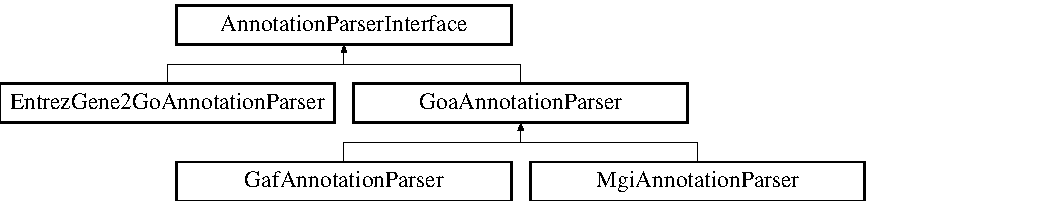
\includegraphics[height=2.705314cm]{classAnnotationParserInterface}
\end{center}
\end{figure}
\subsection*{Public Member Functions}
\begin{DoxyCompactItemize}
\item 
virtual \hyperlink{classAnnotationData}{Annotation\+Data} $\ast$ \hyperlink{classAnnotationParserInterface_a1d5cfb902f088a9cf96fdc6b1e5529ab}{parse\+Annotation\+File} (std\+::string file\+Name)=0
\begin{DoxyCompactList}\small\item\em A pure virtual method for parsing the file and returning an \hyperlink{classAnnotationData}{Annotation\+Data} object. \end{DoxyCompactList}\item 
virtual bool \hyperlink{classAnnotationParserInterface_a5848b37ca77d78213c87cc5aefebf030}{is\+File\+Good} (const std\+::string \&file\+Name)=0
\begin{DoxyCompactList}\small\item\em A pure virtual method for checking if a file exists and is formatted correctly. \end{DoxyCompactList}\item 
virtual \hyperlink{classAnnotationParserInterface}{Annotation\+Parser\+Interface} $\ast$ \hyperlink{classAnnotationParserInterface_a966edeb9aaaa5e94f4c1436afc731a24}{clone} ()=0
\begin{DoxyCompactList}\small\item\em A pure virtual clone function for factory pattern. \end{DoxyCompactList}\end{DoxyCompactItemize}


\subsection{Detailed Description}
An interface class to define annotation parsers. 

This class defines the interface of an annotation parser. Pure virtual methods require that parsers implement these methods. 

\subsection{Member Function Documentation}
\index{Annotation\+Parser\+Interface@{Annotation\+Parser\+Interface}!clone@{clone}}
\index{clone@{clone}!Annotation\+Parser\+Interface@{Annotation\+Parser\+Interface}}
\subsubsection[{\texorpdfstring{clone()=0}{clone()=0}}]{\setlength{\rightskip}{0pt plus 5cm}virtual {\bf Annotation\+Parser\+Interface}$\ast$ Annotation\+Parser\+Interface\+::clone (
\begin{DoxyParamCaption}
{}
\end{DoxyParamCaption}
)\hspace{0.3cm}{\ttfamily [pure virtual]}}\hypertarget{classAnnotationParserInterface_a966edeb9aaaa5e94f4c1436afc731a24}{}\label{classAnnotationParserInterface_a966edeb9aaaa5e94f4c1436afc731a24}


A pure virtual clone function for factory pattern. 

This pure virtual method returns an instance of this interface. This method is used in a factory class to have the ability to decide the parser at runtime. 

Implemented in \hyperlink{classGoaAnnotationParser_a266297bb5a107572c98515f692684369}{Goa\+Annotation\+Parser}, and \hyperlink{classEntrezGene2GoAnnotationParser_a56aaa3a03354c6894fed75accfa2637b}{Entrez\+Gene2\+Go\+Annotation\+Parser}.

\index{Annotation\+Parser\+Interface@{Annotation\+Parser\+Interface}!is\+File\+Good@{is\+File\+Good}}
\index{is\+File\+Good@{is\+File\+Good}!Annotation\+Parser\+Interface@{Annotation\+Parser\+Interface}}
\subsubsection[{\texorpdfstring{is\+File\+Good(const std\+::string \&file\+Name)=0}{isFileGood(const std::string &fileName)=0}}]{\setlength{\rightskip}{0pt plus 5cm}virtual bool Annotation\+Parser\+Interface\+::is\+File\+Good (
\begin{DoxyParamCaption}
\item[{const std\+::string \&}]{file\+Name}
\end{DoxyParamCaption}
)\hspace{0.3cm}{\ttfamily [pure virtual]}}\hypertarget{classAnnotationParserInterface_a5848b37ca77d78213c87cc5aefebf030}{}\label{classAnnotationParserInterface_a5848b37ca77d78213c87cc5aefebf030}


A pure virtual method for checking if a file exists and is formatted correctly. 

This pure virtual function delegates format checking to the implementing class. 

Implemented in \hyperlink{classGoaAnnotationParser_aa8093812131c34de52b084ff2b02abbf}{Goa\+Annotation\+Parser}, and \hyperlink{classEntrezGene2GoAnnotationParser_a5e418ff06c4e2619c0723b828a8578cd}{Entrez\+Gene2\+Go\+Annotation\+Parser}.

\index{Annotation\+Parser\+Interface@{Annotation\+Parser\+Interface}!parse\+Annotation\+File@{parse\+Annotation\+File}}
\index{parse\+Annotation\+File@{parse\+Annotation\+File}!Annotation\+Parser\+Interface@{Annotation\+Parser\+Interface}}
\subsubsection[{\texorpdfstring{parse\+Annotation\+File(std\+::string file\+Name)=0}{parseAnnotationFile(std::string fileName)=0}}]{\setlength{\rightskip}{0pt plus 5cm}virtual {\bf Annotation\+Data}$\ast$ Annotation\+Parser\+Interface\+::parse\+Annotation\+File (
\begin{DoxyParamCaption}
\item[{std\+::string}]{file\+Name}
\end{DoxyParamCaption}
)\hspace{0.3cm}{\ttfamily [pure virtual]}}\hypertarget{classAnnotationParserInterface_a1d5cfb902f088a9cf96fdc6b1e5529ab}{}\label{classAnnotationParserInterface_a1d5cfb902f088a9cf96fdc6b1e5529ab}


A pure virtual method for parsing the file and returning an \hyperlink{classAnnotationData}{Annotation\+Data} object. 

This pure virtual method requires any parser to have a method that takes a filename string and returns an \hyperlink{classAnnotationData}{Annotation\+Data} object pointer. 

Implemented in \hyperlink{classGoaAnnotationParser_a2973e2dcfecea10e09da13ed0ab27dff}{Goa\+Annotation\+Parser}, and \hyperlink{classEntrezGene2GoAnnotationParser_aca2333f3cc25595c1283c3b290dd45cf}{Entrez\+Gene2\+Go\+Annotation\+Parser}.



The documentation for this class was generated from the following file\+:\begin{DoxyCompactItemize}
\item 
ggtk/Annotation\+Parser\+Interface.\+hpp\end{DoxyCompactItemize}

\hypertarget{classBestMatchAverageSetSimilarity}{}\section{Best\+Match\+Average\+Set\+Similarity Class Reference}
\label{classBestMatchAverageSetSimilarity}\index{Best\+Match\+Average\+Set\+Similarity@{Best\+Match\+Average\+Set\+Similarity}}


A class to calculate the best match average similarity between go terms for 2 sets.  




{\ttfamily \#include $<$ggtk/\+Best\+Match\+Average\+Set\+Similarity.\+hpp$>$}

Inheritance diagram for Best\+Match\+Average\+Set\+Similarity\+:\begin{figure}[H]
\begin{center}
\leavevmode
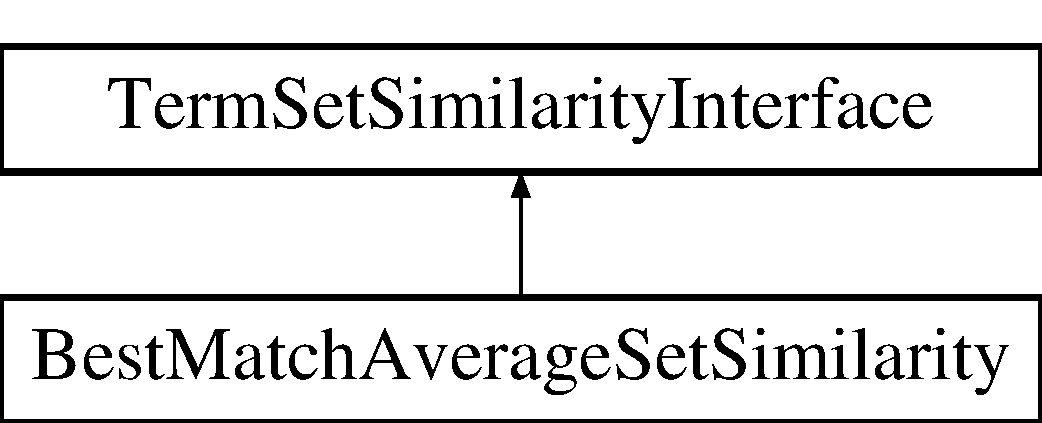
\includegraphics[height=2.000000cm]{classBestMatchAverageSetSimilarity}
\end{center}
\end{figure}
\subsection*{Public Member Functions}
\begin{DoxyCompactItemize}
\item 
\hyperlink{classBestMatchAverageSetSimilarity_afbc85286f64e945d9c3e0bf193171721}{Best\+Match\+Average\+Set\+Similarity} (\hyperlink{classTermSimilarityInterface}{Term\+Similarity\+Interface} $\ast$sim\+Measure)
\begin{DoxyCompactList}\small\item\em Constructor. \end{DoxyCompactList}\item 
double \hyperlink{classBestMatchAverageSetSimilarity_adf1b3109b46f04087f919bdb33e131f0}{calculate\+Similarity} (const boost\+::unordered\+\_\+set$<$ std\+::string $>$ \&termsA, const boost\+::unordered\+\_\+set$<$ std\+::string $>$ \&termsB)
\begin{DoxyCompactList}\small\item\em A method for calculating term set to term set similarity for \hyperlink{namespaceGO}{GO} terms;. \end{DoxyCompactList}\end{DoxyCompactItemize}


\subsection{Detailed Description}
A class to calculate the best match average similarity between go terms for 2 sets. 

This class defines the best match average similarity getween two sets of terms. Used by Couto et al.

F. M. Couto, M. J. Silva, and P. M. Coutinho, \char`\"{}\+Measuring semantic similarity
between Gene Ontology terms,\char`\"{} Data \& Knowledge Engineering, vol. 61, pp. 137-\/152, Apr 2007. 

\subsection{Constructor \& Destructor Documentation}
\index{Best\+Match\+Average\+Set\+Similarity@{Best\+Match\+Average\+Set\+Similarity}!Best\+Match\+Average\+Set\+Similarity@{Best\+Match\+Average\+Set\+Similarity}}
\index{Best\+Match\+Average\+Set\+Similarity@{Best\+Match\+Average\+Set\+Similarity}!Best\+Match\+Average\+Set\+Similarity@{Best\+Match\+Average\+Set\+Similarity}}
\subsubsection[{\texorpdfstring{Best\+Match\+Average\+Set\+Similarity(\+Term\+Similarity\+Interface $\ast$sim\+Measure)}{BestMatchAverageSetSimilarity(TermSimilarityInterface *simMeasure)}}]{\setlength{\rightskip}{0pt plus 5cm}Best\+Match\+Average\+Set\+Similarity\+::\+Best\+Match\+Average\+Set\+Similarity (
\begin{DoxyParamCaption}
\item[{{\bf Term\+Similarity\+Interface} $\ast$}]{sim\+Measure}
\end{DoxyParamCaption}
)\hspace{0.3cm}{\ttfamily [inline]}}\hypertarget{classBestMatchAverageSetSimilarity_afbc85286f64e945d9c3e0bf193171721}{}\label{classBestMatchAverageSetSimilarity_afbc85286f64e945d9c3e0bf193171721}


Constructor. 

Creates the \hyperlink{classBestMatchAverageSetSimilarity}{Best\+Match\+Average\+Set\+Similarity} class assigning the similarity measure private memeber. 

\subsection{Member Function Documentation}
\index{Best\+Match\+Average\+Set\+Similarity@{Best\+Match\+Average\+Set\+Similarity}!calculate\+Similarity@{calculate\+Similarity}}
\index{calculate\+Similarity@{calculate\+Similarity}!Best\+Match\+Average\+Set\+Similarity@{Best\+Match\+Average\+Set\+Similarity}}
\subsubsection[{\texorpdfstring{calculate\+Similarity(const boost\+::unordered\+\_\+set$<$ std\+::string $>$ \&terms\+A, const boost\+::unordered\+\_\+set$<$ std\+::string $>$ \&terms\+B)}{calculateSimilarity(const boost::unordered_set< std::string > &termsA, const boost::unordered_set< std::string > &termsB)}}]{\setlength{\rightskip}{0pt plus 5cm}double Best\+Match\+Average\+Set\+Similarity\+::calculate\+Similarity (
\begin{DoxyParamCaption}
\item[{const boost\+::unordered\+\_\+set$<$ std\+::string $>$ \&}]{termsA, }
\item[{const boost\+::unordered\+\_\+set$<$ std\+::string $>$ \&}]{termsB}
\end{DoxyParamCaption}
)\hspace{0.3cm}{\ttfamily [inline]}, {\ttfamily [virtual]}}\hypertarget{classBestMatchAverageSetSimilarity_adf1b3109b46f04087f919bdb33e131f0}{}\label{classBestMatchAverageSetSimilarity_adf1b3109b46f04087f919bdb33e131f0}


A method for calculating term set to term set similarity for \hyperlink{namespaceGO}{GO} terms;. 

This method returns the best match average similarity. 

Implements \hyperlink{classTermSetSimilarityInterface_aeb985b714efc3df40e55bdd31e425e04}{Term\+Set\+Similarity\+Interface}.



The documentation for this class was generated from the following file\+:\begin{DoxyCompactItemize}
\item 
ggtk/Best\+Match\+Average\+Set\+Similarity.\+hpp\end{DoxyCompactItemize}

\hypertarget{classCoutoGraSMAdjustedSharedInformation}{}\section{Couto\+Gra\+S\+M\+Adjusted\+Shared\+Information Class Reference}
\label{classCoutoGraSMAdjustedSharedInformation}\index{Couto\+Gra\+S\+M\+Adjusted\+Shared\+Information@{Couto\+Gra\+S\+M\+Adjusted\+Shared\+Information}}


A class to calculate shared infromation accross disjoint common ancetors using an adjusted algorithm.  




{\ttfamily \#include $<$ggtk/\+Couto\+Gra\+S\+M\+Adjusted\+Shared\+Information.\+hpp$>$}

Inheritance diagram for Couto\+Gra\+S\+M\+Adjusted\+Shared\+Information\+:\begin{figure}[H]
\begin{center}
\leavevmode
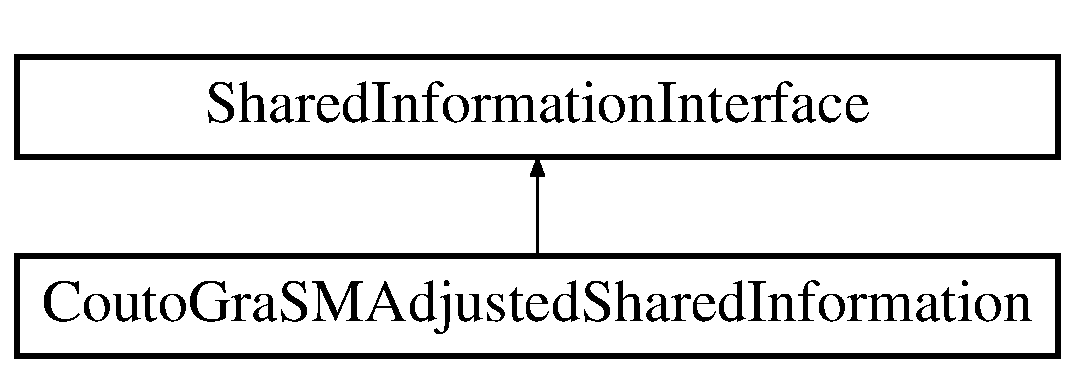
\includegraphics[height=2.000000cm]{classCoutoGraSMAdjustedSharedInformation}
\end{center}
\end{figure}
\subsection*{Public Member Functions}
\begin{DoxyCompactItemize}
\item 
\hyperlink{classCoutoGraSMAdjustedSharedInformation_a4a04a361710cd2d01d684756dfaffdaa}{Couto\+Gra\+S\+M\+Adjusted\+Shared\+Information} (\hyperlink{classGoGraph}{Go\+Graph} $\ast$go\+Graph, \hyperlink{classTermInformationContentMap}{Term\+Information\+Content\+Map} \&ic\+Map)
\begin{DoxyCompactList}\small\item\em Constructor. \end{DoxyCompactList}\item 
boost\+::unordered\+\_\+set$<$ std\+::string $>$ \hyperlink{classCoutoGraSMAdjustedSharedInformation_a1cabbefb71400f4a09a43f2ee772dd13}{get\+Common\+Disjoint\+Ancestors} (const std\+::string \&term\+C1, const std\+::string \&term\+C2)
\begin{DoxyCompactList}\small\item\em Calculate disjunctive ancestors. \end{DoxyCompactList}\item 
bool \hyperlink{classCoutoGraSMAdjustedSharedInformation_a1075d42621e143afd799a88d49964f6e}{is\+Disjoint} (const std\+::string \&termC, const std\+::string \&term\+A1, const std\+::string \&term\+A2)
\begin{DoxyCompactList}\small\item\em Determine if a terms are disjoint in a concept. \end{DoxyCompactList}\item 
std\+::size\+\_\+t \hyperlink{classCoutoGraSMAdjustedSharedInformation_aad9e157135c5d9de7c5e7f49c3d812b4}{get\+Num\+Paths} (const std\+::string \&termA, const std\+::string \&termB)
\begin{DoxyCompactList}\small\item\em Calculate the number of paths between two concept terms. \end{DoxyCompactList}\item 
double \hyperlink{classCoutoGraSMAdjustedSharedInformation_ac93a66e1b8efafc8cd1c166424241af9}{shared\+Information} (const std\+::string \&termA, const std\+::string \&termB)
\begin{DoxyCompactList}\small\item\em Shared infromation between two conecepts. \end{DoxyCompactList}\item 
double \hyperlink{classCoutoGraSMAdjustedSharedInformation_a6a228833a96e710c4e143cefaf364a37}{shared\+Information} (const std\+::string \&term)
\begin{DoxyCompactList}\small\item\em Term information content. \end{DoxyCompactList}\item 
double \hyperlink{classCoutoGraSMAdjustedSharedInformation_ab66e18a4f169878ad2a9e9d6d3feb459}{max\+Information\+Content} (const std\+::string \&term)
\begin{DoxyCompactList}\small\item\em Maximum Ontology IC for normalization. \end{DoxyCompactList}\item 
bool \hyperlink{classCoutoGraSMAdjustedSharedInformation_ae6304b98a7c8784327f978ee59372ca3}{has\+Term} (const std\+::string \&term)
\begin{DoxyCompactList}\small\item\em An interface method for determining if a term can be found. \end{DoxyCompactList}\item 
bool \hyperlink{classCoutoGraSMAdjustedSharedInformation_a9e6387f431eddaf42a1b18529cb3a8f5}{is\+Same\+Ontology} (const std\+::string \&termA, const std\+::string \&termB)
\begin{DoxyCompactList}\small\item\em An interface method for determining if the two terms are of like ontologies. \end{DoxyCompactList}\end{DoxyCompactItemize}


\subsection{Detailed Description}
A class to calculate shared infromation accross disjoint common ancetors using an adjusted algorithm. 

This class calculates shared infromation accross disjoint common ancetors. This is a modificaiton of the original algorithm provided by Couto. The adjustment changes the contrain to path lengths to strictly greater than. See line 150.

F. M. Couto, M. J. Silva, and P. M. Coutinho, \char`\"{}\+Measuring semantic similarity
between Gene Ontology terms,\char`\"{} Data \& Knowledge Engineering, vol. 61, pp. 137-\/152, Apr 2007.

Couto proposing calculating this value a subsituite for the IC of the M\+I\+CA in calculating Resnik, Lin, and Jiang-\/\+Conrath 

\subsection{Constructor \& Destructor Documentation}
\index{Couto\+Gra\+S\+M\+Adjusted\+Shared\+Information@{Couto\+Gra\+S\+M\+Adjusted\+Shared\+Information}!Couto\+Gra\+S\+M\+Adjusted\+Shared\+Information@{Couto\+Gra\+S\+M\+Adjusted\+Shared\+Information}}
\index{Couto\+Gra\+S\+M\+Adjusted\+Shared\+Information@{Couto\+Gra\+S\+M\+Adjusted\+Shared\+Information}!Couto\+Gra\+S\+M\+Adjusted\+Shared\+Information@{Couto\+Gra\+S\+M\+Adjusted\+Shared\+Information}}
\subsubsection[{\texorpdfstring{Couto\+Gra\+S\+M\+Adjusted\+Shared\+Information(\+Go\+Graph $\ast$go\+Graph, Term\+Information\+Content\+Map \&ic\+Map)}{CoutoGraSMAdjustedSharedInformation(GoGraph *goGraph, TermInformationContentMap &icMap)}}]{\setlength{\rightskip}{0pt plus 5cm}Couto\+Gra\+S\+M\+Adjusted\+Shared\+Information\+::\+Couto\+Gra\+S\+M\+Adjusted\+Shared\+Information (
\begin{DoxyParamCaption}
\item[{{\bf Go\+Graph} $\ast$}]{go\+Graph, }
\item[{{\bf Term\+Information\+Content\+Map} \&}]{ic\+Map}
\end{DoxyParamCaption}
)\hspace{0.3cm}{\ttfamily [inline]}}\hypertarget{classCoutoGraSMAdjustedSharedInformation_a4a04a361710cd2d01d684756dfaffdaa}{}\label{classCoutoGraSMAdjustedSharedInformation_a4a04a361710cd2d01d684756dfaffdaa}


Constructor. 

Creates the \hyperlink{classCoutoGraSMAdjustedSharedInformation}{Couto\+Gra\+S\+M\+Adjusted\+Shared\+Information} class 

\subsection{Member Function Documentation}
\index{Couto\+Gra\+S\+M\+Adjusted\+Shared\+Information@{Couto\+Gra\+S\+M\+Adjusted\+Shared\+Information}!get\+Common\+Disjoint\+Ancestors@{get\+Common\+Disjoint\+Ancestors}}
\index{get\+Common\+Disjoint\+Ancestors@{get\+Common\+Disjoint\+Ancestors}!Couto\+Gra\+S\+M\+Adjusted\+Shared\+Information@{Couto\+Gra\+S\+M\+Adjusted\+Shared\+Information}}
\subsubsection[{\texorpdfstring{get\+Common\+Disjoint\+Ancestors(const std\+::string \&term\+C1, const std\+::string \&term\+C2)}{getCommonDisjointAncestors(const std::string &termC1, const std::string &termC2)}}]{\setlength{\rightskip}{0pt plus 5cm}boost\+::unordered\+\_\+set$<$std\+::string$>$ Couto\+Gra\+S\+M\+Adjusted\+Shared\+Information\+::get\+Common\+Disjoint\+Ancestors (
\begin{DoxyParamCaption}
\item[{const std\+::string \&}]{term\+C1, }
\item[{const std\+::string \&}]{term\+C2}
\end{DoxyParamCaption}
)\hspace{0.3cm}{\ttfamily [inline]}}\hypertarget{classCoutoGraSMAdjustedSharedInformation_a1cabbefb71400f4a09a43f2ee772dd13}{}\label{classCoutoGraSMAdjustedSharedInformation_a1cabbefb71400f4a09a43f2ee772dd13}


Calculate disjunctive ancestors. 

A method for determining common disjunctive ancestors for two terms \index{Couto\+Gra\+S\+M\+Adjusted\+Shared\+Information@{Couto\+Gra\+S\+M\+Adjusted\+Shared\+Information}!get\+Num\+Paths@{get\+Num\+Paths}}
\index{get\+Num\+Paths@{get\+Num\+Paths}!Couto\+Gra\+S\+M\+Adjusted\+Shared\+Information@{Couto\+Gra\+S\+M\+Adjusted\+Shared\+Information}}
\subsubsection[{\texorpdfstring{get\+Num\+Paths(const std\+::string \&term\+A, const std\+::string \&term\+B)}{getNumPaths(const std::string &termA, const std::string &termB)}}]{\setlength{\rightskip}{0pt plus 5cm}std\+::size\+\_\+t Couto\+Gra\+S\+M\+Adjusted\+Shared\+Information\+::get\+Num\+Paths (
\begin{DoxyParamCaption}
\item[{const std\+::string \&}]{termA, }
\item[{const std\+::string \&}]{termB}
\end{DoxyParamCaption}
)\hspace{0.3cm}{\ttfamily [inline]}}\hypertarget{classCoutoGraSMAdjustedSharedInformation_aad9e157135c5d9de7c5e7f49c3d812b4}{}\label{classCoutoGraSMAdjustedSharedInformation_aad9e157135c5d9de7c5e7f49c3d812b4}


Calculate the number of paths between two concept terms. 

A method for calculating the number of paths from one term to another. \index{Couto\+Gra\+S\+M\+Adjusted\+Shared\+Information@{Couto\+Gra\+S\+M\+Adjusted\+Shared\+Information}!has\+Term@{has\+Term}}
\index{has\+Term@{has\+Term}!Couto\+Gra\+S\+M\+Adjusted\+Shared\+Information@{Couto\+Gra\+S\+M\+Adjusted\+Shared\+Information}}
\subsubsection[{\texorpdfstring{has\+Term(const std\+::string \&term)}{hasTerm(const std::string &term)}}]{\setlength{\rightskip}{0pt plus 5cm}bool Couto\+Gra\+S\+M\+Adjusted\+Shared\+Information\+::has\+Term (
\begin{DoxyParamCaption}
\item[{const std\+::string \&}]{term}
\end{DoxyParamCaption}
)\hspace{0.3cm}{\ttfamily [inline]}, {\ttfamily [virtual]}}\hypertarget{classCoutoGraSMAdjustedSharedInformation_ae6304b98a7c8784327f978ee59372ca3}{}\label{classCoutoGraSMAdjustedSharedInformation_ae6304b98a7c8784327f978ee59372ca3}


An interface method for determining if a term can be found. 

Determines if the term can be found in the current map. 

Implements \hyperlink{classSharedInformationInterface_a3f056cf6a40eea8c1669108087dcd5c8}{Shared\+Information\+Interface}.

\index{Couto\+Gra\+S\+M\+Adjusted\+Shared\+Information@{Couto\+Gra\+S\+M\+Adjusted\+Shared\+Information}!is\+Disjoint@{is\+Disjoint}}
\index{is\+Disjoint@{is\+Disjoint}!Couto\+Gra\+S\+M\+Adjusted\+Shared\+Information@{Couto\+Gra\+S\+M\+Adjusted\+Shared\+Information}}
\subsubsection[{\texorpdfstring{is\+Disjoint(const std\+::string \&term\+C, const std\+::string \&term\+A1, const std\+::string \&term\+A2)}{isDisjoint(const std::string &termC, const std::string &termA1, const std::string &termA2)}}]{\setlength{\rightskip}{0pt plus 5cm}bool Couto\+Gra\+S\+M\+Adjusted\+Shared\+Information\+::is\+Disjoint (
\begin{DoxyParamCaption}
\item[{const std\+::string \&}]{termC, }
\item[{const std\+::string \&}]{term\+A1, }
\item[{const std\+::string \&}]{term\+A2}
\end{DoxyParamCaption}
)\hspace{0.3cm}{\ttfamily [inline]}}\hypertarget{classCoutoGraSMAdjustedSharedInformation_a1075d42621e143afd799a88d49964f6e}{}\label{classCoutoGraSMAdjustedSharedInformation_a1075d42621e143afd799a88d49964f6e}


Determine if a terms are disjoint in a concept. 

A method for determining if, for a term c, a pair (a1,a2) is disjoint in c \index{Couto\+Gra\+S\+M\+Adjusted\+Shared\+Information@{Couto\+Gra\+S\+M\+Adjusted\+Shared\+Information}!is\+Same\+Ontology@{is\+Same\+Ontology}}
\index{is\+Same\+Ontology@{is\+Same\+Ontology}!Couto\+Gra\+S\+M\+Adjusted\+Shared\+Information@{Couto\+Gra\+S\+M\+Adjusted\+Shared\+Information}}
\subsubsection[{\texorpdfstring{is\+Same\+Ontology(const std\+::string \&term\+A, const std\+::string \&term\+B)}{isSameOntology(const std::string &termA, const std::string &termB)}}]{\setlength{\rightskip}{0pt plus 5cm}bool Couto\+Gra\+S\+M\+Adjusted\+Shared\+Information\+::is\+Same\+Ontology (
\begin{DoxyParamCaption}
\item[{const std\+::string \&}]{termA, }
\item[{const std\+::string \&}]{termB}
\end{DoxyParamCaption}
)\hspace{0.3cm}{\ttfamily [inline]}, {\ttfamily [virtual]}}\hypertarget{classCoutoGraSMAdjustedSharedInformation_a9e6387f431eddaf42a1b18529cb3a8f5}{}\label{classCoutoGraSMAdjustedSharedInformation_a9e6387f431eddaf42a1b18529cb3a8f5}


An interface method for determining if the two terms are of like ontologies. 

Determine if two terms are of the same ontology. 

Implements \hyperlink{classSharedInformationInterface_a607463b9736df9c4b8ec3ba9fe41c19d}{Shared\+Information\+Interface}.

\index{Couto\+Gra\+S\+M\+Adjusted\+Shared\+Information@{Couto\+Gra\+S\+M\+Adjusted\+Shared\+Information}!max\+Information\+Content@{max\+Information\+Content}}
\index{max\+Information\+Content@{max\+Information\+Content}!Couto\+Gra\+S\+M\+Adjusted\+Shared\+Information@{Couto\+Gra\+S\+M\+Adjusted\+Shared\+Information}}
\subsubsection[{\texorpdfstring{max\+Information\+Content(const std\+::string \&term)}{maxInformationContent(const std::string &term)}}]{\setlength{\rightskip}{0pt plus 5cm}double Couto\+Gra\+S\+M\+Adjusted\+Shared\+Information\+::max\+Information\+Content (
\begin{DoxyParamCaption}
\item[{const std\+::string \&}]{term}
\end{DoxyParamCaption}
)\hspace{0.3cm}{\ttfamily [inline]}, {\ttfamily [virtual]}}\hypertarget{classCoutoGraSMAdjustedSharedInformation_ab66e18a4f169878ad2a9e9d6d3feb459}{}\label{classCoutoGraSMAdjustedSharedInformation_ab66e18a4f169878ad2a9e9d6d3feb459}


Maximum Ontology IC for normalization. 

An interface method for returning the maximum information content for a term within a corpus for normalization purposes. 

Implements \hyperlink{classSharedInformationInterface_a7356ba99509458777972ce0f00ebd999}{Shared\+Information\+Interface}.

\index{Couto\+Gra\+S\+M\+Adjusted\+Shared\+Information@{Couto\+Gra\+S\+M\+Adjusted\+Shared\+Information}!shared\+Information@{shared\+Information}}
\index{shared\+Information@{shared\+Information}!Couto\+Gra\+S\+M\+Adjusted\+Shared\+Information@{Couto\+Gra\+S\+M\+Adjusted\+Shared\+Information}}
\subsubsection[{\texorpdfstring{shared\+Information(const std\+::string \&term\+A, const std\+::string \&term\+B)}{sharedInformation(const std::string &termA, const std::string &termB)}}]{\setlength{\rightskip}{0pt plus 5cm}double Couto\+Gra\+S\+M\+Adjusted\+Shared\+Information\+::shared\+Information (
\begin{DoxyParamCaption}
\item[{const std\+::string \&}]{termA, }
\item[{const std\+::string \&}]{termB}
\end{DoxyParamCaption}
)\hspace{0.3cm}{\ttfamily [inline]}, {\ttfamily [virtual]}}\hypertarget{classCoutoGraSMAdjustedSharedInformation_ac93a66e1b8efafc8cd1c166424241af9}{}\label{classCoutoGraSMAdjustedSharedInformation_ac93a66e1b8efafc8cd1c166424241af9}


Shared infromation between two conecepts. 

A method for calculating the shared infromation between two concepts. 

Implements \hyperlink{classSharedInformationInterface_a76e8858eb598442b86b0fd3be1c519e7}{Shared\+Information\+Interface}.

\index{Couto\+Gra\+S\+M\+Adjusted\+Shared\+Information@{Couto\+Gra\+S\+M\+Adjusted\+Shared\+Information}!shared\+Information@{shared\+Information}}
\index{shared\+Information@{shared\+Information}!Couto\+Gra\+S\+M\+Adjusted\+Shared\+Information@{Couto\+Gra\+S\+M\+Adjusted\+Shared\+Information}}
\subsubsection[{\texorpdfstring{shared\+Information(const std\+::string \&term)}{sharedInformation(const std::string &term)}}]{\setlength{\rightskip}{0pt plus 5cm}double Couto\+Gra\+S\+M\+Adjusted\+Shared\+Information\+::shared\+Information (
\begin{DoxyParamCaption}
\item[{const std\+::string \&}]{term}
\end{DoxyParamCaption}
)\hspace{0.3cm}{\ttfamily [inline]}, {\ttfamily [virtual]}}\hypertarget{classCoutoGraSMAdjustedSharedInformation_a6a228833a96e710c4e143cefaf364a37}{}\label{classCoutoGraSMAdjustedSharedInformation_a6a228833a96e710c4e143cefaf364a37}


Term information content. 

An interface method to conventiently get information content of a single term 

Implements \hyperlink{classSharedInformationInterface_aba102c0e44fbc098baef6074f1eb37b6}{Shared\+Information\+Interface}.



The documentation for this class was generated from the following file\+:\begin{DoxyCompactItemize}
\item 
ggtk/Couto\+Gra\+S\+M\+Adjusted\+Shared\+Information.\+hpp\end{DoxyCompactItemize}

\hypertarget{classCoutoGraSMSharedInformation}{}\section{Couto\+Gra\+S\+M\+Shared\+Information Class Reference}
\label{classCoutoGraSMSharedInformation}\index{Couto\+Gra\+S\+M\+Shared\+Information@{Couto\+Gra\+S\+M\+Shared\+Information}}


A class to calculate shared infromation accross disjoint common ancetors using the exact algorithm as written in the paper.  




{\ttfamily \#include $<$ggtk/\+Couto\+Gra\+S\+M\+Shared\+Information.\+hpp$>$}

Inheritance diagram for Couto\+Gra\+S\+M\+Shared\+Information\+:\begin{figure}[H]
\begin{center}
\leavevmode
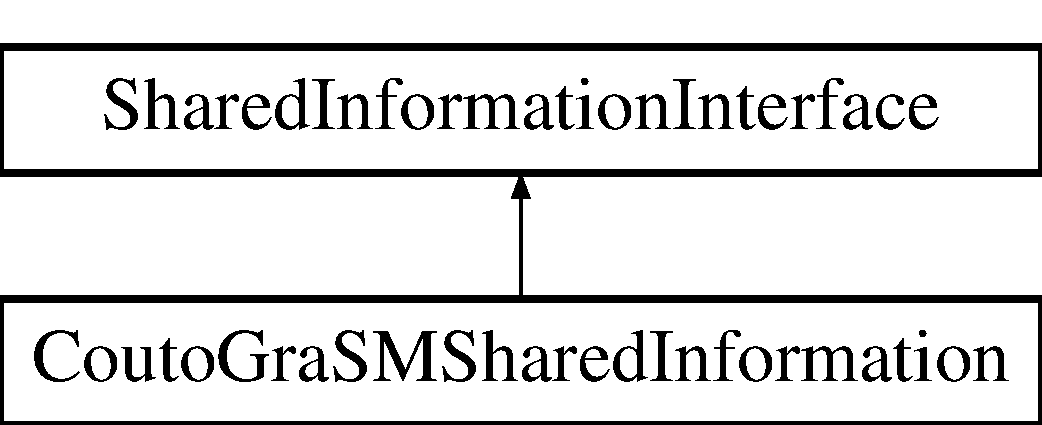
\includegraphics[height=2.000000cm]{classCoutoGraSMSharedInformation}
\end{center}
\end{figure}
\subsection*{Public Member Functions}
\begin{DoxyCompactItemize}
\item 
\hyperlink{classCoutoGraSMSharedInformation_a8e923a60f27eca7922a628a9efd7afdc}{Couto\+Gra\+S\+M\+Shared\+Information} (\hyperlink{classGoGraph}{Go\+Graph} $\ast$go\+Graph, \hyperlink{classTermInformationContentMap}{Term\+Information\+Content\+Map} \&ic\+Map)
\begin{DoxyCompactList}\small\item\em A constructor. \end{DoxyCompactList}\item 
boost\+::unordered\+\_\+set$<$ std\+::string $>$ \hyperlink{classCoutoGraSMSharedInformation_ac1dd8eacbfde6f724b11f4b276e41faf}{get\+Common\+Disjoint\+Ancestors} (const std\+::string \&term\+C1, const std\+::string \&term\+C2)
\begin{DoxyCompactList}\small\item\em A method for determining the common disjunctive ancestors. \end{DoxyCompactList}\item 
bool \hyperlink{classCoutoGraSMSharedInformation_aa935c6e99178b043fd4dbc8f2e4ba29d}{is\+Disjoint} (const std\+::string \&termC, const std\+::string \&term\+A1, const std\+::string \&term\+A2)
\begin{DoxyCompactList}\small\item\em A method for determining if for a term c, a pair (a1,a2) is disjoint in c. \end{DoxyCompactList}\item 
std\+::size\+\_\+t \hyperlink{classCoutoGraSMSharedInformation_abbb7cbdc8131eaab6d5b467fcb1ecd8a}{get\+Num\+Paths} (const std\+::string \&termA, const std\+::string \&termB)
\begin{DoxyCompactList}\small\item\em A method for calculating the number of paths for one term to another. \end{DoxyCompactList}\item 
double \hyperlink{classCoutoGraSMSharedInformation_aeb3ea4684e5f198464ce9354171981d3}{shared\+Information} (const std\+::string \&termA, const std\+::string \&termB)
\begin{DoxyCompactList}\small\item\em An method for returning the shared information of two terms. \end{DoxyCompactList}\item 
double \hyperlink{classCoutoGraSMSharedInformation_a1c9a0a709b77822cd3bc967beed08b66}{shared\+Information} (const std\+::string \&term)
\begin{DoxyCompactList}\small\item\em An interface method for returning the shared information of a single terms,or information content. \end{DoxyCompactList}\item 
double \hyperlink{classCoutoGraSMSharedInformation_ae97d2b59ecd6d1eeee2583c6005c65a2}{max\+Information\+Content} (const std\+::string \&term)
\begin{DoxyCompactList}\small\item\em An interface method for returning the maximum information content for a term. \end{DoxyCompactList}\item 
bool \hyperlink{classCoutoGraSMSharedInformation_a718055d6fecea9e10125ae4895af7f95}{has\+Term} (const std\+::string \&term)
\begin{DoxyCompactList}\small\item\em An interface method for determining if a term can be found. \end{DoxyCompactList}\item 
bool \hyperlink{classCoutoGraSMSharedInformation_ae6e12a30f03b0c2232d73277d8d47cd1}{is\+Same\+Ontology} (const std\+::string \&termA, const std\+::string \&termB)
\begin{DoxyCompactList}\small\item\em An interface method for determining if the two terms are of like ontologies. \end{DoxyCompactList}\end{DoxyCompactItemize}


\subsection{Detailed Description}
A class to calculate shared infromation accross disjoint common ancetors using the exact algorithm as written in the paper. 

This class calculates shared infromation accross disjoint common ancetors.

F. M. Couto, M. J. Silva, and P. M. Coutinho, \char`\"{}\+Measuring semantic similarity
between Gene Ontology terms,\char`\"{} Data \& Knowledge Engineering, vol. 61, pp. 137-\/152, Apr 2007.

Couto proposing calculating this value a subsituite for the IC of the M\+I\+CA in calculating Resnik, Lin, and Jiang-\/\+Conrath 

\subsection{Constructor \& Destructor Documentation}
\index{Couto\+Gra\+S\+M\+Shared\+Information@{Couto\+Gra\+S\+M\+Shared\+Information}!Couto\+Gra\+S\+M\+Shared\+Information@{Couto\+Gra\+S\+M\+Shared\+Information}}
\index{Couto\+Gra\+S\+M\+Shared\+Information@{Couto\+Gra\+S\+M\+Shared\+Information}!Couto\+Gra\+S\+M\+Shared\+Information@{Couto\+Gra\+S\+M\+Shared\+Information}}
\subsubsection[{\texorpdfstring{Couto\+Gra\+S\+M\+Shared\+Information(\+Go\+Graph $\ast$go\+Graph, Term\+Information\+Content\+Map \&ic\+Map)}{CoutoGraSMSharedInformation(GoGraph *goGraph, TermInformationContentMap &icMap)}}]{\setlength{\rightskip}{0pt plus 5cm}Couto\+Gra\+S\+M\+Shared\+Information\+::\+Couto\+Gra\+S\+M\+Shared\+Information (
\begin{DoxyParamCaption}
\item[{{\bf Go\+Graph} $\ast$}]{go\+Graph, }
\item[{{\bf Term\+Information\+Content\+Map} \&}]{ic\+Map}
\end{DoxyParamCaption}
)\hspace{0.3cm}{\ttfamily [inline]}}\hypertarget{classCoutoGraSMSharedInformation_a8e923a60f27eca7922a628a9efd7afdc}{}\label{classCoutoGraSMSharedInformation_a8e923a60f27eca7922a628a9efd7afdc}


A constructor. 

Creates the Couto\+Gra\+S\+M\+Greater\+Or\+Equal class 

\subsection{Member Function Documentation}
\index{Couto\+Gra\+S\+M\+Shared\+Information@{Couto\+Gra\+S\+M\+Shared\+Information}!get\+Common\+Disjoint\+Ancestors@{get\+Common\+Disjoint\+Ancestors}}
\index{get\+Common\+Disjoint\+Ancestors@{get\+Common\+Disjoint\+Ancestors}!Couto\+Gra\+S\+M\+Shared\+Information@{Couto\+Gra\+S\+M\+Shared\+Information}}
\subsubsection[{\texorpdfstring{get\+Common\+Disjoint\+Ancestors(const std\+::string \&term\+C1, const std\+::string \&term\+C2)}{getCommonDisjointAncestors(const std::string &termC1, const std::string &termC2)}}]{\setlength{\rightskip}{0pt plus 5cm}boost\+::unordered\+\_\+set$<$std\+::string$>$ Couto\+Gra\+S\+M\+Shared\+Information\+::get\+Common\+Disjoint\+Ancestors (
\begin{DoxyParamCaption}
\item[{const std\+::string \&}]{term\+C1, }
\item[{const std\+::string \&}]{term\+C2}
\end{DoxyParamCaption}
)\hspace{0.3cm}{\ttfamily [inline]}}\hypertarget{classCoutoGraSMSharedInformation_ac1dd8eacbfde6f724b11f4b276e41faf}{}\label{classCoutoGraSMSharedInformation_ac1dd8eacbfde6f724b11f4b276e41faf}


A method for determining the common disjunctive ancestors. 

This method returns the common disjunctive ancestors for two terms \index{Couto\+Gra\+S\+M\+Shared\+Information@{Couto\+Gra\+S\+M\+Shared\+Information}!get\+Num\+Paths@{get\+Num\+Paths}}
\index{get\+Num\+Paths@{get\+Num\+Paths}!Couto\+Gra\+S\+M\+Shared\+Information@{Couto\+Gra\+S\+M\+Shared\+Information}}
\subsubsection[{\texorpdfstring{get\+Num\+Paths(const std\+::string \&term\+A, const std\+::string \&term\+B)}{getNumPaths(const std::string &termA, const std::string &termB)}}]{\setlength{\rightskip}{0pt plus 5cm}std\+::size\+\_\+t Couto\+Gra\+S\+M\+Shared\+Information\+::get\+Num\+Paths (
\begin{DoxyParamCaption}
\item[{const std\+::string \&}]{termA, }
\item[{const std\+::string \&}]{termB}
\end{DoxyParamCaption}
)\hspace{0.3cm}{\ttfamily [inline]}}\hypertarget{classCoutoGraSMSharedInformation_abbb7cbdc8131eaab6d5b467fcb1ecd8a}{}\label{classCoutoGraSMSharedInformation_abbb7cbdc8131eaab6d5b467fcb1ecd8a}


A method for calculating the number of paths for one term to another. 

This method returns the number of paths between two terms \index{Couto\+Gra\+S\+M\+Shared\+Information@{Couto\+Gra\+S\+M\+Shared\+Information}!has\+Term@{has\+Term}}
\index{has\+Term@{has\+Term}!Couto\+Gra\+S\+M\+Shared\+Information@{Couto\+Gra\+S\+M\+Shared\+Information}}
\subsubsection[{\texorpdfstring{has\+Term(const std\+::string \&term)}{hasTerm(const std::string &term)}}]{\setlength{\rightskip}{0pt plus 5cm}bool Couto\+Gra\+S\+M\+Shared\+Information\+::has\+Term (
\begin{DoxyParamCaption}
\item[{const std\+::string \&}]{term}
\end{DoxyParamCaption}
)\hspace{0.3cm}{\ttfamily [inline]}, {\ttfamily [virtual]}}\hypertarget{classCoutoGraSMSharedInformation_a718055d6fecea9e10125ae4895af7f95}{}\label{classCoutoGraSMSharedInformation_a718055d6fecea9e10125ae4895af7f95}


An interface method for determining if a term can be found. 

Determines if the term can be found in the current map. 

Implements \hyperlink{classSharedInformationInterface_a3f056cf6a40eea8c1669108087dcd5c8}{Shared\+Information\+Interface}.

\index{Couto\+Gra\+S\+M\+Shared\+Information@{Couto\+Gra\+S\+M\+Shared\+Information}!is\+Disjoint@{is\+Disjoint}}
\index{is\+Disjoint@{is\+Disjoint}!Couto\+Gra\+S\+M\+Shared\+Information@{Couto\+Gra\+S\+M\+Shared\+Information}}
\subsubsection[{\texorpdfstring{is\+Disjoint(const std\+::string \&term\+C, const std\+::string \&term\+A1, const std\+::string \&term\+A2)}{isDisjoint(const std::string &termC, const std::string &termA1, const std::string &termA2)}}]{\setlength{\rightskip}{0pt plus 5cm}bool Couto\+Gra\+S\+M\+Shared\+Information\+::is\+Disjoint (
\begin{DoxyParamCaption}
\item[{const std\+::string \&}]{termC, }
\item[{const std\+::string \&}]{term\+A1, }
\item[{const std\+::string \&}]{term\+A2}
\end{DoxyParamCaption}
)\hspace{0.3cm}{\ttfamily [inline]}}\hypertarget{classCoutoGraSMSharedInformation_aa935c6e99178b043fd4dbc8f2e4ba29d}{}\label{classCoutoGraSMSharedInformation_aa935c6e99178b043fd4dbc8f2e4ba29d}


A method for determining if for a term c, a pair (a1,a2) is disjoint in c. 

This method returns \index{Couto\+Gra\+S\+M\+Shared\+Information@{Couto\+Gra\+S\+M\+Shared\+Information}!is\+Same\+Ontology@{is\+Same\+Ontology}}
\index{is\+Same\+Ontology@{is\+Same\+Ontology}!Couto\+Gra\+S\+M\+Shared\+Information@{Couto\+Gra\+S\+M\+Shared\+Information}}
\subsubsection[{\texorpdfstring{is\+Same\+Ontology(const std\+::string \&term\+A, const std\+::string \&term\+B)}{isSameOntology(const std::string &termA, const std::string &termB)}}]{\setlength{\rightskip}{0pt plus 5cm}bool Couto\+Gra\+S\+M\+Shared\+Information\+::is\+Same\+Ontology (
\begin{DoxyParamCaption}
\item[{const std\+::string \&}]{termA, }
\item[{const std\+::string \&}]{termB}
\end{DoxyParamCaption}
)\hspace{0.3cm}{\ttfamily [inline]}, {\ttfamily [virtual]}}\hypertarget{classCoutoGraSMSharedInformation_ae6e12a30f03b0c2232d73277d8d47cd1}{}\label{classCoutoGraSMSharedInformation_ae6e12a30f03b0c2232d73277d8d47cd1}


An interface method for determining if the two terms are of like ontologies. 

Determine if two terms are of the same ontology. 

Implements \hyperlink{classSharedInformationInterface_a607463b9736df9c4b8ec3ba9fe41c19d}{Shared\+Information\+Interface}.

\index{Couto\+Gra\+S\+M\+Shared\+Information@{Couto\+Gra\+S\+M\+Shared\+Information}!max\+Information\+Content@{max\+Information\+Content}}
\index{max\+Information\+Content@{max\+Information\+Content}!Couto\+Gra\+S\+M\+Shared\+Information@{Couto\+Gra\+S\+M\+Shared\+Information}}
\subsubsection[{\texorpdfstring{max\+Information\+Content(const std\+::string \&term)}{maxInformationContent(const std::string &term)}}]{\setlength{\rightskip}{0pt plus 5cm}double Couto\+Gra\+S\+M\+Shared\+Information\+::max\+Information\+Content (
\begin{DoxyParamCaption}
\item[{const std\+::string \&}]{term}
\end{DoxyParamCaption}
)\hspace{0.3cm}{\ttfamily [inline]}, {\ttfamily [virtual]}}\hypertarget{classCoutoGraSMSharedInformation_ae97d2b59ecd6d1eeee2583c6005c65a2}{}\label{classCoutoGraSMSharedInformation_ae97d2b59ecd6d1eeee2583c6005c65a2}


An interface method for returning the maximum information content for a term. 

This method provides the absolute max information content within a corpus for normalization purposes. 

Implements \hyperlink{classSharedInformationInterface_a7356ba99509458777972ce0f00ebd999}{Shared\+Information\+Interface}.

\index{Couto\+Gra\+S\+M\+Shared\+Information@{Couto\+Gra\+S\+M\+Shared\+Information}!shared\+Information@{shared\+Information}}
\index{shared\+Information@{shared\+Information}!Couto\+Gra\+S\+M\+Shared\+Information@{Couto\+Gra\+S\+M\+Shared\+Information}}
\subsubsection[{\texorpdfstring{shared\+Information(const std\+::string \&term\+A, const std\+::string \&term\+B)}{sharedInformation(const std::string &termA, const std::string &termB)}}]{\setlength{\rightskip}{0pt plus 5cm}double Couto\+Gra\+S\+M\+Shared\+Information\+::shared\+Information (
\begin{DoxyParamCaption}
\item[{const std\+::string \&}]{termA, }
\item[{const std\+::string \&}]{termB}
\end{DoxyParamCaption}
)\hspace{0.3cm}{\ttfamily [inline]}, {\ttfamily [virtual]}}\hypertarget{classCoutoGraSMSharedInformation_aeb3ea4684e5f198464ce9354171981d3}{}\label{classCoutoGraSMSharedInformation_aeb3ea4684e5f198464ce9354171981d3}


An method for returning the shared information of two terms. 

This method returns the mean information content disjoint common ancestors 

Implements \hyperlink{classSharedInformationInterface_a76e8858eb598442b86b0fd3be1c519e7}{Shared\+Information\+Interface}.

\index{Couto\+Gra\+S\+M\+Shared\+Information@{Couto\+Gra\+S\+M\+Shared\+Information}!shared\+Information@{shared\+Information}}
\index{shared\+Information@{shared\+Information}!Couto\+Gra\+S\+M\+Shared\+Information@{Couto\+Gra\+S\+M\+Shared\+Information}}
\subsubsection[{\texorpdfstring{shared\+Information(const std\+::string \&term)}{sharedInformation(const std::string &term)}}]{\setlength{\rightskip}{0pt plus 5cm}double Couto\+Gra\+S\+M\+Shared\+Information\+::shared\+Information (
\begin{DoxyParamCaption}
\item[{const std\+::string \&}]{term}
\end{DoxyParamCaption}
)\hspace{0.3cm}{\ttfamily [inline]}, {\ttfamily [virtual]}}\hypertarget{classCoutoGraSMSharedInformation_a1c9a0a709b77822cd3bc967beed08b66}{}\label{classCoutoGraSMSharedInformation_a1c9a0a709b77822cd3bc967beed08b66}


An interface method for returning the shared information of a single terms,or information content. 

This method privdes a mechanism for returing a term\textquotesingle{}s infromation content. 

Implements \hyperlink{classSharedInformationInterface_aba102c0e44fbc098baef6074f1eb37b6}{Shared\+Information\+Interface}.



The documentation for this class was generated from the following file\+:\begin{DoxyCompactItemize}
\item 
ggtk/Couto\+Gra\+S\+M\+Shared\+Information.\+hpp\end{DoxyCompactItemize}

\hypertarget{classTermProbabilityMap_1_1dfs__cumulative__annotations__visitor}{}\section{Term\+Probability\+Map\+:\+:dfs\+\_\+cumulative\+\_\+annotations\+\_\+visitor Class Reference}
\label{classTermProbabilityMap_1_1dfs__cumulative__annotations__visitor}\index{Term\+Probability\+Map\+::dfs\+\_\+cumulative\+\_\+annotations\+\_\+visitor@{Term\+Probability\+Map\+::dfs\+\_\+cumulative\+\_\+annotations\+\_\+visitor}}


Depth first search boost visitor.  




{\ttfamily \#include $<$ggtk/\+Term\+Probability\+Map.\+hpp$>$}

Inheritance diagram for Term\+Probability\+Map\+:\+:dfs\+\_\+cumulative\+\_\+annotations\+\_\+visitor\+:\begin{figure}[H]
\begin{center}
\leavevmode
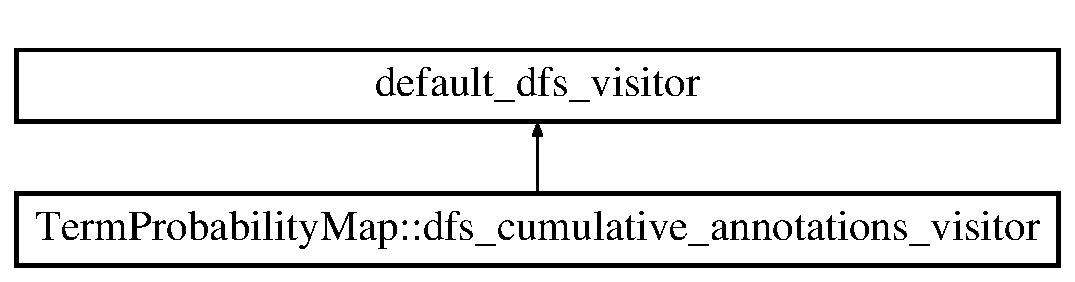
\includegraphics[height=2.000000cm]{classTermProbabilityMap_1_1dfs__cumulative__annotations__visitor}
\end{center}
\end{figure}
\subsection*{Public Member Functions}
\begin{DoxyCompactItemize}
\item 
\hyperlink{classTermProbabilityMap_1_1dfs__cumulative__annotations__visitor_a3c6b493a2f9b5b966f12c947553ffbd2}{dfs\+\_\+cumulative\+\_\+annotations\+\_\+visitor} (\hyperlink{classGoGraph}{Go\+Graph} $\ast$in\+Graph, \hyperlink{classAnnotationData}{Annotation\+Data} $\ast$in\+Data, std\+::vector$<$ std\+::size\+\_\+t $>$ $\ast$annotations, boost\+::unordered\+\_\+map$<$ std\+::string, std\+::size\+\_\+t $>$ $\ast$name\+To\+Index)\hypertarget{classTermProbabilityMap_1_1dfs__cumulative__annotations__visitor_a3c6b493a2f9b5b966f12c947553ffbd2}{}\label{classTermProbabilityMap_1_1dfs__cumulative__annotations__visitor_a3c6b493a2f9b5b966f12c947553ffbd2}

\begin{DoxyCompactList}\small\item\em A parameterized constructor passing parameters to the boost default\+\_\+dfs\+\_\+visitor. \end{DoxyCompactList}\item 
{\footnotesize template$<$typename Vertex , typename Graph $>$ }\\void \hyperlink{classTermProbabilityMap_1_1dfs__cumulative__annotations__visitor_ac6147a4c2bcfe83492667b248630a525}{finish\+\_\+vertex} (Vertex u, const Graph \&g)
\begin{DoxyCompactList}\small\item\em The extended method of the default\+\_\+dfs\+\_\+visitor, finish\+\_\+vertex. \end{DoxyCompactList}\end{DoxyCompactItemize}
\subsection*{Public Attributes}
\begin{DoxyCompactItemize}
\item 
\hyperlink{classGoGraph}{Go\+Graph} $\ast$ \hyperlink{classTermProbabilityMap_1_1dfs__cumulative__annotations__visitor_a9588ad34b2d743cb8245c91d27fe22e1}{go\+Graph}\hypertarget{classTermProbabilityMap_1_1dfs__cumulative__annotations__visitor_a9588ad34b2d743cb8245c91d27fe22e1}{}\label{classTermProbabilityMap_1_1dfs__cumulative__annotations__visitor_a9588ad34b2d743cb8245c91d27fe22e1}

\begin{DoxyCompactList}\small\item\em The go graph object. \end{DoxyCompactList}\item 
\hyperlink{classAnnotationData}{Annotation\+Data} $\ast$ \hyperlink{classTermProbabilityMap_1_1dfs__cumulative__annotations__visitor_a2200329f595bd75534fb37be72550d21}{anno\+Data}\hypertarget{classTermProbabilityMap_1_1dfs__cumulative__annotations__visitor_a2200329f595bd75534fb37be72550d21}{}\label{classTermProbabilityMap_1_1dfs__cumulative__annotations__visitor_a2200329f595bd75534fb37be72550d21}

\begin{DoxyCompactList}\small\item\em An \hyperlink{classAnnotationData}{Annotation\+Data} object for accessing annotations. \end{DoxyCompactList}\item 
std\+::vector$<$ std\+::size\+\_\+t $>$ $\ast$ \hyperlink{classTermProbabilityMap_1_1dfs__cumulative__annotations__visitor_aab2aba55afae7c48e8834d409a889193}{anno\+List}\hypertarget{classTermProbabilityMap_1_1dfs__cumulative__annotations__visitor_aab2aba55afae7c48e8834d409a889193}{}\label{classTermProbabilityMap_1_1dfs__cumulative__annotations__visitor_aab2aba55afae7c48e8834d409a889193}

\begin{DoxyCompactList}\small\item\em The annotaiton list to hold the and query the cummulative annotations. \end{DoxyCompactList}\item 
boost\+::unordered\+\_\+map$<$ std\+::string, std\+::size\+\_\+t $>$ $\ast$ \hyperlink{classTermProbabilityMap_1_1dfs__cumulative__annotations__visitor_af1db06d68d0e336e1300aabc2ba5ad9c}{name\+Index\+Map}\hypertarget{classTermProbabilityMap_1_1dfs__cumulative__annotations__visitor_af1db06d68d0e336e1300aabc2ba5ad9c}{}\label{classTermProbabilityMap_1_1dfs__cumulative__annotations__visitor_af1db06d68d0e336e1300aabc2ba5ad9c}

\begin{DoxyCompactList}\small\item\em A map from name To index, initialized in this visitor. \end{DoxyCompactList}\end{DoxyCompactItemize}


\subsection{Detailed Description}
Depth first search boost visitor. 

This defines a class used by Term\+Proability\+Map to calculate the cumulative annotations of a term based on the true path rule. Basically this class is passed to a boost Depth first search algorithm to add the number of a child\textquotesingle{}s annotaitons to the parent. 

\subsection{Member Function Documentation}
\index{Term\+Probability\+Map\+::dfs\+\_\+cumulative\+\_\+annotations\+\_\+visitor@{Term\+Probability\+Map\+::dfs\+\_\+cumulative\+\_\+annotations\+\_\+visitor}!finish\+\_\+vertex@{finish\+\_\+vertex}}
\index{finish\+\_\+vertex@{finish\+\_\+vertex}!Term\+Probability\+Map\+::dfs\+\_\+cumulative\+\_\+annotations\+\_\+visitor@{Term\+Probability\+Map\+::dfs\+\_\+cumulative\+\_\+annotations\+\_\+visitor}}
\subsubsection[{\texorpdfstring{finish\+\_\+vertex(\+Vertex u, const Graph \&g)}{finish_vertex(Vertex u, const Graph &g)}}]{\setlength{\rightskip}{0pt plus 5cm}template$<$typename Vertex , typename Graph $>$ void Term\+Probability\+Map\+::dfs\+\_\+cumulative\+\_\+annotations\+\_\+visitor\+::finish\+\_\+vertex (
\begin{DoxyParamCaption}
\item[{Vertex}]{u, }
\item[{const Graph \&}]{g}
\end{DoxyParamCaption}
)\hspace{0.3cm}{\ttfamily [inline]}}\hypertarget{classTermProbabilityMap_1_1dfs__cumulative__annotations__visitor_ac6147a4c2bcfe83492667b248630a525}{}\label{classTermProbabilityMap_1_1dfs__cumulative__annotations__visitor_ac6147a4c2bcfe83492667b248630a525}


The extended method of the default\+\_\+dfs\+\_\+visitor, finish\+\_\+vertex. 

This method is called during a depth first search traversal of a graph and called when the visitor finished or leaves a node. This is the last time the algorithm touches the node.

Here we calculate the number of cummulative annotations for a term (node) by adding the current term\textquotesingle{}s annotations to the annotations of the term\textquotesingle{}s children. 

The documentation for this class was generated from the following file\+:\begin{DoxyCompactItemize}
\item 
ggtk/Term\+Probability\+Map.\+hpp\end{DoxyCompactItemize}

\hypertarget{classDisallowedSetEvidencePolicy}{}\section{Disallowed\+Set\+Evidence\+Policy Class Reference}
\label{classDisallowedSetEvidencePolicy}\index{Disallowed\+Set\+Evidence\+Policy@{Disallowed\+Set\+Evidence\+Policy}}


A class to allow only a set of evidence codes for annotations.  




{\ttfamily \#include $<$ggtk/\+Disallowed\+Set\+Evidence\+Policy.\+hpp$>$}

Inheritance diagram for Disallowed\+Set\+Evidence\+Policy\+:\begin{figure}[H]
\begin{center}
\leavevmode
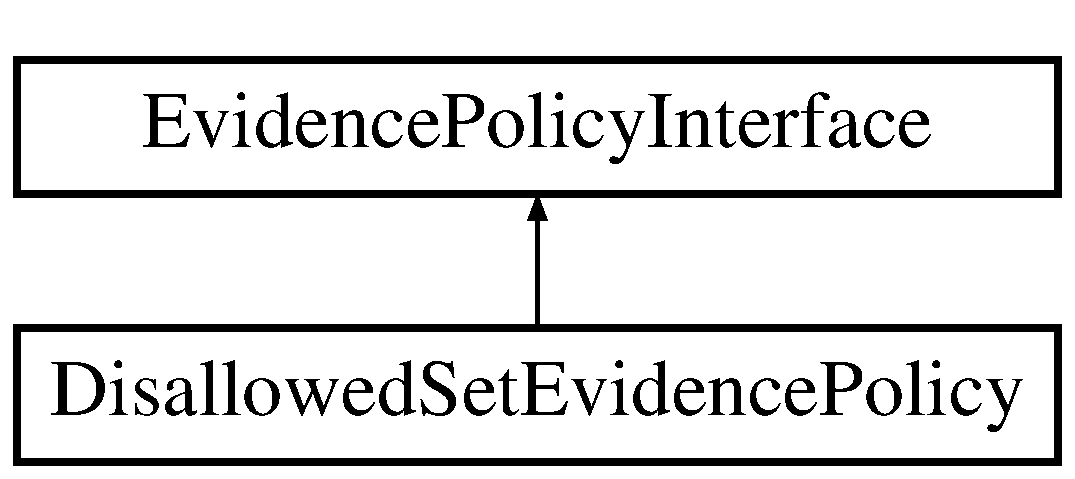
\includegraphics[height=2.000000cm]{classDisallowedSetEvidencePolicy}
\end{center}
\end{figure}
\subsection*{Public Member Functions}
\begin{DoxyCompactItemize}
\item 
\hyperlink{classDisallowedSetEvidencePolicy_a4db63ff71aa72c7744187a36099e5b09}{Disallowed\+Set\+Evidence\+Policy} ()
\begin{DoxyCompactList}\small\item\em A constructor. \end{DoxyCompactList}\item 
\hyperlink{classDisallowedSetEvidencePolicy_a50c8885e5a3abf0a3110492f07e21268}{Disallowed\+Set\+Evidence\+Policy} (std\+::vector$<$ \hyperlink{namespaceGO_a4ce5387bbcdaec3648957c7903f2caf3}{G\+O\+::\+Evidence\+Code} $>$ evidence\+Codes)
\begin{DoxyCompactList}\small\item\em A parameterized constructor. \end{DoxyCompactList}\item 
bool \hyperlink{classDisallowedSetEvidencePolicy_aaa0959ad33624b4d418d57d286c41852}{is\+Allowed} (\hyperlink{namespaceGO_a4ce5387bbcdaec3648957c7903f2caf3}{G\+O\+::\+Evidence\+Code} evidence\+Code)
\begin{DoxyCompactList}\small\item\em a method to test if an eviddence code is allowed or not \end{DoxyCompactList}\item 
void \hyperlink{classDisallowedSetEvidencePolicy_a565f023aa750687b96206608d17cf392}{add\+Evidence} (\hyperlink{namespaceGO_a4ce5387bbcdaec3648957c7903f2caf3}{G\+O\+::\+Evidence\+Code} evidence\+Code)
\begin{DoxyCompactList}\small\item\em a method to add a evidence to the set of evidence codes not allowed \end{DoxyCompactList}\item 
void \hyperlink{classDisallowedSetEvidencePolicy_ab3ccdee816e866886e77aaf1c5129ae8}{add\+Evidence} (const std\+::string \&string\+Code)
\begin{DoxyCompactList}\small\item\em a method to add a evidence to the set of evidence codes allowed \end{DoxyCompactList}\item 
bool \hyperlink{classDisallowedSetEvidencePolicy_ac913c46a483b9c163099ce5b2128b881}{is\+Empty} ()
\begin{DoxyCompactList}\small\item\em a method to determine if the Policy is empty, disallowed set is never empty \end{DoxyCompactList}\end{DoxyCompactItemize}


\subsection{Detailed Description}
A class to allow only a set of evidence codes for annotations. 

A class to allow only certain evidence codes in the go graph. It uses a set of enums to restric the types of evidence codes considered for annotations. 

\subsection{Constructor \& Destructor Documentation}
\index{Disallowed\+Set\+Evidence\+Policy@{Disallowed\+Set\+Evidence\+Policy}!Disallowed\+Set\+Evidence\+Policy@{Disallowed\+Set\+Evidence\+Policy}}
\index{Disallowed\+Set\+Evidence\+Policy@{Disallowed\+Set\+Evidence\+Policy}!Disallowed\+Set\+Evidence\+Policy@{Disallowed\+Set\+Evidence\+Policy}}
\subsubsection[{\texorpdfstring{Disallowed\+Set\+Evidence\+Policy()}{DisallowedSetEvidencePolicy()}}]{\setlength{\rightskip}{0pt plus 5cm}Disallowed\+Set\+Evidence\+Policy\+::\+Disallowed\+Set\+Evidence\+Policy (
\begin{DoxyParamCaption}
{}
\end{DoxyParamCaption}
)\hspace{0.3cm}{\ttfamily [inline]}}\hypertarget{classDisallowedSetEvidencePolicy_a4db63ff71aa72c7744187a36099e5b09}{}\label{classDisallowedSetEvidencePolicy_a4db63ff71aa72c7744187a36099e5b09}


A constructor. 

Creates the default(empty) \hyperlink{classDisallowedSetEvidencePolicy}{Disallowed\+Set\+Evidence\+Policy} \index{Disallowed\+Set\+Evidence\+Policy@{Disallowed\+Set\+Evidence\+Policy}!Disallowed\+Set\+Evidence\+Policy@{Disallowed\+Set\+Evidence\+Policy}}
\index{Disallowed\+Set\+Evidence\+Policy@{Disallowed\+Set\+Evidence\+Policy}!Disallowed\+Set\+Evidence\+Policy@{Disallowed\+Set\+Evidence\+Policy}}
\subsubsection[{\texorpdfstring{Disallowed\+Set\+Evidence\+Policy(std\+::vector$<$ G\+O\+::\+Evidence\+Code $>$ evidence\+Codes)}{DisallowedSetEvidencePolicy(std::vector< GO::EvidenceCode > evidenceCodes)}}]{\setlength{\rightskip}{0pt plus 5cm}Disallowed\+Set\+Evidence\+Policy\+::\+Disallowed\+Set\+Evidence\+Policy (
\begin{DoxyParamCaption}
\item[{std\+::vector$<$ {\bf G\+O\+::\+Evidence\+Code} $>$}]{evidence\+Codes}
\end{DoxyParamCaption}
)\hspace{0.3cm}{\ttfamily [inline]}}\hypertarget{classDisallowedSetEvidencePolicy_a50c8885e5a3abf0a3110492f07e21268}{}\label{classDisallowedSetEvidencePolicy_a50c8885e5a3abf0a3110492f07e21268}


A parameterized constructor. 

Creats the \hyperlink{classDisallowedSetEvidencePolicy}{Disallowed\+Set\+Evidence\+Policy} using a list(vector) of evidence codes to allow 

\subsection{Member Function Documentation}
\index{Disallowed\+Set\+Evidence\+Policy@{Disallowed\+Set\+Evidence\+Policy}!add\+Evidence@{add\+Evidence}}
\index{add\+Evidence@{add\+Evidence}!Disallowed\+Set\+Evidence\+Policy@{Disallowed\+Set\+Evidence\+Policy}}
\subsubsection[{\texorpdfstring{add\+Evidence(\+G\+O\+::\+Evidence\+Code evidence\+Code)}{addEvidence(GO::EvidenceCode evidenceCode)}}]{\setlength{\rightskip}{0pt plus 5cm}void Disallowed\+Set\+Evidence\+Policy\+::add\+Evidence (
\begin{DoxyParamCaption}
\item[{{\bf G\+O\+::\+Evidence\+Code}}]{evidence\+Code}
\end{DoxyParamCaption}
)\hspace{0.3cm}{\ttfamily [inline]}}\hypertarget{classDisallowedSetEvidencePolicy_a565f023aa750687b96206608d17cf392}{}\label{classDisallowedSetEvidencePolicy_a565f023aa750687b96206608d17cf392}


a method to add a evidence to the set of evidence codes not allowed 

adds a evidence to the set of evidence codes not allowed \index{Disallowed\+Set\+Evidence\+Policy@{Disallowed\+Set\+Evidence\+Policy}!add\+Evidence@{add\+Evidence}}
\index{add\+Evidence@{add\+Evidence}!Disallowed\+Set\+Evidence\+Policy@{Disallowed\+Set\+Evidence\+Policy}}
\subsubsection[{\texorpdfstring{add\+Evidence(const std\+::string \&string\+Code)}{addEvidence(const std::string &stringCode)}}]{\setlength{\rightskip}{0pt plus 5cm}void Disallowed\+Set\+Evidence\+Policy\+::add\+Evidence (
\begin{DoxyParamCaption}
\item[{const std\+::string \&}]{string\+Code}
\end{DoxyParamCaption}
)\hspace{0.3cm}{\ttfamily [inline]}}\hypertarget{classDisallowedSetEvidencePolicy_ab3ccdee816e866886e77aaf1c5129ae8}{}\label{classDisallowedSetEvidencePolicy_ab3ccdee816e866886e77aaf1c5129ae8}


a method to add a evidence to the set of evidence codes allowed 

adds a evidence to the set of evidence codes allowed by setting its mapped value to true \index{Disallowed\+Set\+Evidence\+Policy@{Disallowed\+Set\+Evidence\+Policy}!is\+Allowed@{is\+Allowed}}
\index{is\+Allowed@{is\+Allowed}!Disallowed\+Set\+Evidence\+Policy@{Disallowed\+Set\+Evidence\+Policy}}
\subsubsection[{\texorpdfstring{is\+Allowed(\+G\+O\+::\+Evidence\+Code evidence\+Code)}{isAllowed(GO::EvidenceCode evidenceCode)}}]{\setlength{\rightskip}{0pt plus 5cm}bool Disallowed\+Set\+Evidence\+Policy\+::is\+Allowed (
\begin{DoxyParamCaption}
\item[{{\bf G\+O\+::\+Evidence\+Code}}]{evidence\+Code}
\end{DoxyParamCaption}
)\hspace{0.3cm}{\ttfamily [inline]}, {\ttfamily [virtual]}}\hypertarget{classDisallowedSetEvidencePolicy_aaa0959ad33624b4d418d57d286c41852}{}\label{classDisallowedSetEvidencePolicy_aaa0959ad33624b4d418d57d286c41852}


a method to test if an eviddence code is allowed or not 

tests if the evidence is allowed. Overridden to fulfill the \hyperlink{classEvidencePolicyInterface}{Evidence\+Policy\+Interface}. This class disallows a set and so returns false if the evidence code is found. 

Implements \hyperlink{classEvidencePolicyInterface_a432d20dd05ec54db46a452ae8d6be4a7}{Evidence\+Policy\+Interface}.

\index{Disallowed\+Set\+Evidence\+Policy@{Disallowed\+Set\+Evidence\+Policy}!is\+Empty@{is\+Empty}}
\index{is\+Empty@{is\+Empty}!Disallowed\+Set\+Evidence\+Policy@{Disallowed\+Set\+Evidence\+Policy}}
\subsubsection[{\texorpdfstring{is\+Empty()}{isEmpty()}}]{\setlength{\rightskip}{0pt plus 5cm}bool Disallowed\+Set\+Evidence\+Policy\+::is\+Empty (
\begin{DoxyParamCaption}
{}
\end{DoxyParamCaption}
)\hspace{0.3cm}{\ttfamily [inline]}}\hypertarget{classDisallowedSetEvidencePolicy_ac913c46a483b9c163099ce5b2128b881}{}\label{classDisallowedSetEvidencePolicy_ac913c46a483b9c163099ce5b2128b881}


a method to determine if the Policy is empty, disallowed set is never empty 

Determines if the Policy is empty 

The documentation for this class was generated from the following file\+:\begin{DoxyCompactItemize}
\item 
ggtk/Disallowed\+Set\+Evidence\+Policy.\+hpp\end{DoxyCompactItemize}

\hypertarget{structGoGraph_1_1EdgeProps}{}\section{Go\+Graph\+:\+:Edge\+Props Struct Reference}
\label{structGoGraph_1_1EdgeProps}\index{Go\+Graph\+::\+Edge\+Props@{Go\+Graph\+::\+Edge\+Props}}


An Edge Property object.  




{\ttfamily \#include $<$ggtk/\+Go\+Graph.\+hpp$>$}

\subsection*{Public Member Functions}
\begin{DoxyCompactItemize}
\item 
\hyperlink{structGoGraph_1_1EdgeProps_ae86950a82bf50040fa0b2c83d7a89fc6}{$\sim$\+Edge\+Props} ()
\end{DoxyCompactItemize}
\subsection*{Public Attributes}
\begin{DoxyCompactItemize}
\item 
\hyperlink{namespaceGO_aaa3905b2e000a8be411da8038827f993}{G\+O\+::\+Relationship} \hyperlink{structGoGraph_1_1EdgeProps_af9336fa93d326a88970e8dafa64fa85e}{rel\+Type}
\end{DoxyCompactItemize}


\subsection{Detailed Description}
An Edge Property object. 

This struct represent the data needed by each edge. Boost provides constant time access to these members by querying them using the vertex and graph objects (graph\+Var\mbox{[}edge\mbox{]}.rel\+Type). 

\subsection{Constructor \& Destructor Documentation}
\index{Go\+Graph\+::\+Edge\+Props@{Go\+Graph\+::\+Edge\+Props}!````~Edge\+Props@{$\sim$\+Edge\+Props}}
\index{````~Edge\+Props@{$\sim$\+Edge\+Props}!Go\+Graph\+::\+Edge\+Props@{Go\+Graph\+::\+Edge\+Props}}
\subsubsection[{\texorpdfstring{$\sim$\+Edge\+Props()}{~EdgeProps()}}]{\setlength{\rightskip}{0pt plus 5cm}Go\+Graph\+::\+Edge\+Props\+::$\sim$\+Edge\+Props (
\begin{DoxyParamCaption}
{}
\end{DoxyParamCaption}
)\hspace{0.3cm}{\ttfamily [inline]}}\hypertarget{structGoGraph_1_1EdgeProps_ae86950a82bf50040fa0b2c83d7a89fc6}{}\label{structGoGraph_1_1EdgeProps_ae86950a82bf50040fa0b2c83d7a89fc6}
Desctructor 

\subsection{Member Data Documentation}
\index{Go\+Graph\+::\+Edge\+Props@{Go\+Graph\+::\+Edge\+Props}!rel\+Type@{rel\+Type}}
\index{rel\+Type@{rel\+Type}!Go\+Graph\+::\+Edge\+Props@{Go\+Graph\+::\+Edge\+Props}}
\subsubsection[{\texorpdfstring{rel\+Type}{relType}}]{\setlength{\rightskip}{0pt plus 5cm}{\bf G\+O\+::\+Relationship} Go\+Graph\+::\+Edge\+Props\+::rel\+Type}\hypertarget{structGoGraph_1_1EdgeProps_af9336fa93d326a88970e8dafa64fa85e}{}\label{structGoGraph_1_1EdgeProps_af9336fa93d326a88970e8dafa64fa85e}
The type of relationship between the terms, is\+\_\+a, part\+\_\+of etc. 

The documentation for this struct was generated from the following file\+:\begin{DoxyCompactItemize}
\item 
ggtk/Go\+Graph.\+hpp\end{DoxyCompactItemize}

\hypertarget{classEntrezGene2GoAnnotationParser}{}\section{Entrez\+Gene2\+Go\+Annotation\+Parser Class Reference}
\label{classEntrezGene2GoAnnotationParser}\index{Entrez\+Gene2\+Go\+Annotation\+Parser@{Entrez\+Gene2\+Go\+Annotation\+Parser}}


A class to parse an Entrez gene2go annotation file.  




{\ttfamily \#include $<$ggtk/\+Entrez\+Gene2\+Go\+Annotation\+Parser.\+hpp$>$}

Inheritance diagram for Entrez\+Gene2\+Go\+Annotation\+Parser\+:\begin{figure}[H]
\begin{center}
\leavevmode
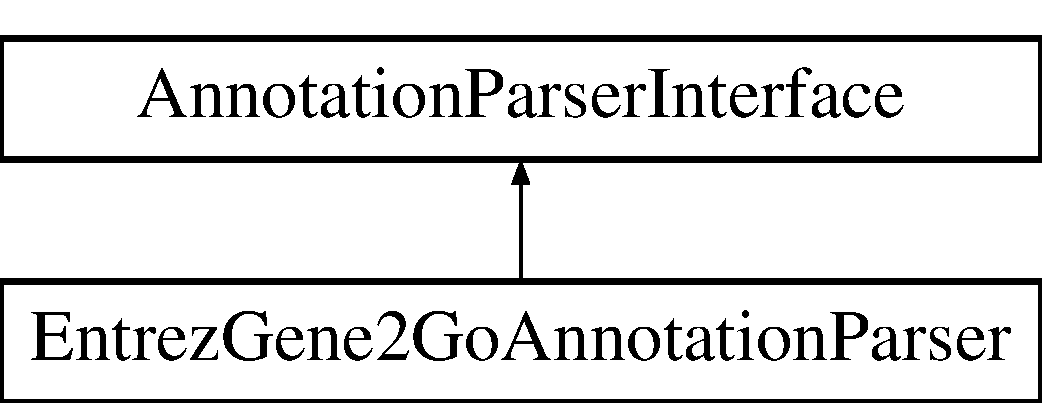
\includegraphics[height=2.000000cm]{classEntrezGene2GoAnnotationParser}
\end{center}
\end{figure}
\subsection*{Public Member Functions}
\begin{DoxyCompactItemize}
\item 
\hyperlink{classAnnotationData}{Annotation\+Data} $\ast$ \hyperlink{classEntrezGene2GoAnnotationParser_aca2333f3cc25595c1283c3b290dd45cf}{parse\+Annotation\+File} (std\+::string filename)
\begin{DoxyCompactList}\small\item\em An interface method for parsing an annotation file. \end{DoxyCompactList}\item 
bool \hyperlink{classEntrezGene2GoAnnotationParser_a5e418ff06c4e2619c0723b828a8578cd}{is\+File\+Good} (const std\+::string \&file\+Name)
\begin{DoxyCompactList}\small\item\em A method for checking if a file exists and is formatted correctly. \end{DoxyCompactList}\item 
\hyperlink{classAnnotationParserInterface}{Annotation\+Parser\+Interface} $\ast$ \hyperlink{classEntrezGene2GoAnnotationParser_a56aaa3a03354c6894fed75accfa2637b}{clone} ()
\begin{DoxyCompactList}\small\item\em An interface method for creating a new instance of the parser. \end{DoxyCompactList}\item 
\hyperlink{classEntrezGene2GoAnnotationParser_ad9fad52a10bd767ff769ee4d953bda3d}{Entrez\+Gene2\+Go\+Annotation\+Parser} (\hyperlink{classEvidencePolicyInterface}{Evidence\+Policy\+Interface} $\ast$policy)
\begin{DoxyCompactList}\small\item\em A parameterized constructor method for creating the parser with a policy. \end{DoxyCompactList}\item 
\hyperlink{classEntrezGene2GoAnnotationParser_a50b77b0894f628df64ab3104a99e7f3c}{Entrez\+Gene2\+Go\+Annotation\+Parser} ()
\begin{DoxyCompactList}\small\item\em A default constructor method for creating the parser with the default policy. \end{DoxyCompactList}\end{DoxyCompactItemize}


\subsection{Detailed Description}
A class to parse an Entrez gene2go annotation file. 

This class will read an Entrez gene2go file and add those annoations to an \hyperlink{classAnnotationData}{Annotation\+Data} class. Available at\+: \href{ftp://ftp.ncbi.nih.gov/gene/DATA/}{\tt ftp\+://ftp.\+ncbi.\+nih.\+gov/gene/\+D\+A\+T\+A/}

Implements \hyperlink{classAnnotationParserInterface}{Annotation\+Parser\+Interface} 

\subsection{Constructor \& Destructor Documentation}
\index{Entrez\+Gene2\+Go\+Annotation\+Parser@{Entrez\+Gene2\+Go\+Annotation\+Parser}!Entrez\+Gene2\+Go\+Annotation\+Parser@{Entrez\+Gene2\+Go\+Annotation\+Parser}}
\index{Entrez\+Gene2\+Go\+Annotation\+Parser@{Entrez\+Gene2\+Go\+Annotation\+Parser}!Entrez\+Gene2\+Go\+Annotation\+Parser@{Entrez\+Gene2\+Go\+Annotation\+Parser}}
\subsubsection[{\texorpdfstring{Entrez\+Gene2\+Go\+Annotation\+Parser(\+Evidence\+Policy\+Interface $\ast$policy)}{EntrezGene2GoAnnotationParser(EvidencePolicyInterface *policy)}}]{\setlength{\rightskip}{0pt plus 5cm}Entrez\+Gene2\+Go\+Annotation\+Parser\+::\+Entrez\+Gene2\+Go\+Annotation\+Parser (
\begin{DoxyParamCaption}
\item[{{\bf Evidence\+Policy\+Interface} $\ast$}]{policy}
\end{DoxyParamCaption}
)\hspace{0.3cm}{\ttfamily [inline]}}\hypertarget{classEntrezGene2GoAnnotationParser_ad9fad52a10bd767ff769ee4d953bda3d}{}\label{classEntrezGene2GoAnnotationParser_ad9fad52a10bd767ff769ee4d953bda3d}


A parameterized constructor method for creating the parser with a policy. 

Creates the parser \index{Entrez\+Gene2\+Go\+Annotation\+Parser@{Entrez\+Gene2\+Go\+Annotation\+Parser}!Entrez\+Gene2\+Go\+Annotation\+Parser@{Entrez\+Gene2\+Go\+Annotation\+Parser}}
\index{Entrez\+Gene2\+Go\+Annotation\+Parser@{Entrez\+Gene2\+Go\+Annotation\+Parser}!Entrez\+Gene2\+Go\+Annotation\+Parser@{Entrez\+Gene2\+Go\+Annotation\+Parser}}
\subsubsection[{\texorpdfstring{Entrez\+Gene2\+Go\+Annotation\+Parser()}{EntrezGene2GoAnnotationParser()}}]{\setlength{\rightskip}{0pt plus 5cm}Entrez\+Gene2\+Go\+Annotation\+Parser\+::\+Entrez\+Gene2\+Go\+Annotation\+Parser (
\begin{DoxyParamCaption}
{}
\end{DoxyParamCaption}
)\hspace{0.3cm}{\ttfamily [inline]}}\hypertarget{classEntrezGene2GoAnnotationParser_a50b77b0894f628df64ab3104a99e7f3c}{}\label{classEntrezGene2GoAnnotationParser_a50b77b0894f628df64ab3104a99e7f3c}


A default constructor method for creating the parser with the default policy. 

Creates the parser with the default evidence policy, everything is allowed. 

\subsection{Member Function Documentation}
\index{Entrez\+Gene2\+Go\+Annotation\+Parser@{Entrez\+Gene2\+Go\+Annotation\+Parser}!clone@{clone}}
\index{clone@{clone}!Entrez\+Gene2\+Go\+Annotation\+Parser@{Entrez\+Gene2\+Go\+Annotation\+Parser}}
\subsubsection[{\texorpdfstring{clone()}{clone()}}]{\setlength{\rightskip}{0pt plus 5cm}{\bf Annotation\+Parser\+Interface}$\ast$ Entrez\+Gene2\+Go\+Annotation\+Parser\+::clone (
\begin{DoxyParamCaption}
{}
\end{DoxyParamCaption}
)\hspace{0.3cm}{\ttfamily [inline]}, {\ttfamily [virtual]}}\hypertarget{classEntrezGene2GoAnnotationParser_a56aaa3a03354c6894fed75accfa2637b}{}\label{classEntrezGene2GoAnnotationParser_a56aaa3a03354c6894fed75accfa2637b}


An interface method for creating a new instance of the parser. 

This method returns a new instance of the class. This method partially fulfills the interface contract. 

Implements \hyperlink{classAnnotationParserInterface_a966edeb9aaaa5e94f4c1436afc731a24}{Annotation\+Parser\+Interface}.

\index{Entrez\+Gene2\+Go\+Annotation\+Parser@{Entrez\+Gene2\+Go\+Annotation\+Parser}!is\+File\+Good@{is\+File\+Good}}
\index{is\+File\+Good@{is\+File\+Good}!Entrez\+Gene2\+Go\+Annotation\+Parser@{Entrez\+Gene2\+Go\+Annotation\+Parser}}
\subsubsection[{\texorpdfstring{is\+File\+Good(const std\+::string \&file\+Name)}{isFileGood(const std::string &fileName)}}]{\setlength{\rightskip}{0pt plus 5cm}bool Entrez\+Gene2\+Go\+Annotation\+Parser\+::is\+File\+Good (
\begin{DoxyParamCaption}
\item[{const std\+::string \&}]{file\+Name}
\end{DoxyParamCaption}
)\hspace{0.3cm}{\ttfamily [inline]}, {\ttfamily [virtual]}}\hypertarget{classEntrezGene2GoAnnotationParser_a5e418ff06c4e2619c0723b828a8578cd}{}\label{classEntrezGene2GoAnnotationParser_a5e418ff06c4e2619c0723b828a8578cd}


A method for checking if a file exists and is formatted correctly. 

This function checks that the file exists and its format can be recognized. 

Implements \hyperlink{classAnnotationParserInterface_a5848b37ca77d78213c87cc5aefebf030}{Annotation\+Parser\+Interface}.

\index{Entrez\+Gene2\+Go\+Annotation\+Parser@{Entrez\+Gene2\+Go\+Annotation\+Parser}!parse\+Annotation\+File@{parse\+Annotation\+File}}
\index{parse\+Annotation\+File@{parse\+Annotation\+File}!Entrez\+Gene2\+Go\+Annotation\+Parser@{Entrez\+Gene2\+Go\+Annotation\+Parser}}
\subsubsection[{\texorpdfstring{parse\+Annotation\+File(std\+::string filename)}{parseAnnotationFile(std::string filename)}}]{\setlength{\rightskip}{0pt plus 5cm}{\bf Annotation\+Data}$\ast$ Entrez\+Gene2\+Go\+Annotation\+Parser\+::parse\+Annotation\+File (
\begin{DoxyParamCaption}
\item[{std\+::string}]{filename}
\end{DoxyParamCaption}
)\hspace{0.3cm}{\ttfamily [inline]}, {\ttfamily [virtual]}}\hypertarget{classEntrezGene2GoAnnotationParser_aca2333f3cc25595c1283c3b290dd45cf}{}\label{classEntrezGene2GoAnnotationParser_aca2333f3cc25595c1283c3b290dd45cf}


An interface method for parsing an annotation file. 

This method takes a filename as in put and returns a pointer to an \hyperlink{classAnnotationData}{Annotation\+Data} object. This method fulfills part of the interface contract. 

Implements \hyperlink{classAnnotationParserInterface_a1d5cfb902f088a9cf96fdc6b1e5529ab}{Annotation\+Parser\+Interface}.



The documentation for this class was generated from the following file\+:\begin{DoxyCompactItemize}
\item 
ggtk/Entrez\+Gene2\+Go\+Annotation\+Parser.\+hpp\end{DoxyCompactItemize}

\hypertarget{classEvidencePolicyInterface}{}\section{Evidence\+Policy\+Interface Class Reference}
\label{classEvidencePolicyInterface}\index{Evidence\+Policy\+Interface@{Evidence\+Policy\+Interface}}


An interface to check evidence codes for \hyperlink{namespaceGO}{GO} annotations.  




{\ttfamily \#include $<$ggtk/\+Evidence\+Policy\+Interface.\+hpp$>$}

Inheritance diagram for Evidence\+Policy\+Interface\+:\begin{figure}[H]
\begin{center}
\leavevmode
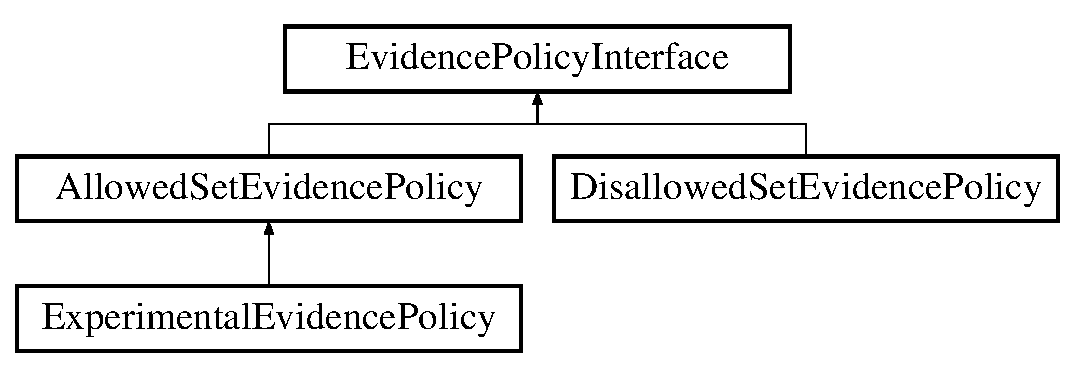
\includegraphics[height=3.000000cm]{classEvidencePolicyInterface}
\end{center}
\end{figure}
\subsection*{Public Member Functions}
\begin{DoxyCompactItemize}
\item 
virtual bool \hyperlink{classEvidencePolicyInterface_a432d20dd05ec54db46a452ae8d6be4a7}{is\+Allowed} (\hyperlink{namespaceGO_a4ce5387bbcdaec3648957c7903f2caf3}{G\+O\+::\+Evidence\+Code} evidence\+Code)=0
\begin{DoxyCompactList}\small\item\em A pure virtual method to test if an evidence code is allowed. \end{DoxyCompactList}\end{DoxyCompactItemize}


\subsection{Detailed Description}
An interface to check evidence codes for \hyperlink{namespaceGO}{GO} annotations. 

This is interface is used to create parsers which will only use a specific set of evidence codes when parsing annotations 

\subsection{Member Function Documentation}
\index{Evidence\+Policy\+Interface@{Evidence\+Policy\+Interface}!is\+Allowed@{is\+Allowed}}
\index{is\+Allowed@{is\+Allowed}!Evidence\+Policy\+Interface@{Evidence\+Policy\+Interface}}
\subsubsection[{\texorpdfstring{is\+Allowed(\+G\+O\+::\+Evidence\+Code evidence\+Code)=0}{isAllowed(GO::EvidenceCode evidenceCode)=0}}]{\setlength{\rightskip}{0pt plus 5cm}virtual bool Evidence\+Policy\+Interface\+::is\+Allowed (
\begin{DoxyParamCaption}
\item[{{\bf G\+O\+::\+Evidence\+Code}}]{evidence\+Code}
\end{DoxyParamCaption}
)\hspace{0.3cm}{\ttfamily [pure virtual]}}\hypertarget{classEvidencePolicyInterface_a432d20dd05ec54db46a452ae8d6be4a7}{}\label{classEvidencePolicyInterface_a432d20dd05ec54db46a452ae8d6be4a7}


A pure virtual method to test if an evidence code is allowed. 

This pure virtual method requires any subclass to imlement an is\+Allowed method to enforce the evidence pollicy. 

Implemented in \hyperlink{classAllowedSetEvidencePolicy_a5979a55da22e57d2faffaa0bdb77457b}{Allowed\+Set\+Evidence\+Policy}, and \hyperlink{classDisallowedSetEvidencePolicy_aaa0959ad33624b4d418d57d286c41852}{Disallowed\+Set\+Evidence\+Policy}.



The documentation for this class was generated from the following file\+:\begin{DoxyCompactItemize}
\item 
ggtk/Evidence\+Policy\+Interface.\+hpp\end{DoxyCompactItemize}

\hypertarget{classExclusivelyInheritedSharedInformation}{}\section{Exclusively\+Inherited\+Shared\+Information Class Reference}
\label{classExclusivelyInheritedSharedInformation}\index{Exclusively\+Inherited\+Shared\+Information@{Exclusively\+Inherited\+Shared\+Information}}


A class to calculate shared infromation in linear time after Zhang and Lai.  




{\ttfamily \#include $<$ggtk/\+Exclusively\+Inherited\+Shared\+Information.\+hpp$>$}

Inheritance diagram for Exclusively\+Inherited\+Shared\+Information\+:\begin{figure}[H]
\begin{center}
\leavevmode
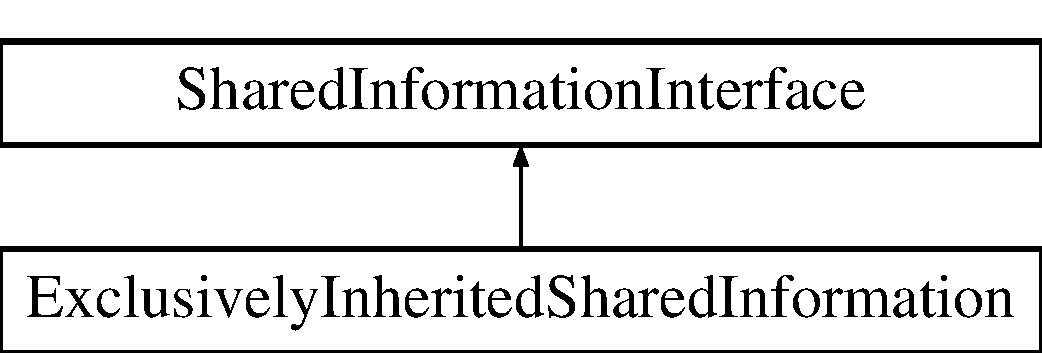
\includegraphics[height=2.000000cm]{classExclusivelyInheritedSharedInformation}
\end{center}
\end{figure}
\subsection*{Public Member Functions}
\begin{DoxyCompactItemize}
\item 
\hyperlink{classExclusivelyInheritedSharedInformation_a176bde96479ad6ea0baba4a520b7038e}{Exclusively\+Inherited\+Shared\+Information} (\hyperlink{classGoGraph}{Go\+Graph} $\ast$go\+Graph, \hyperlink{classTermInformationContentMap}{Term\+Information\+Content\+Map} \&ic\+Map)
\begin{DoxyCompactList}\small\item\em A constructor. \end{DoxyCompactList}\item 
boost\+::unordered\+\_\+set$<$ std\+::string $>$ \hyperlink{classExclusivelyInheritedSharedInformation_a16a51c8f3bd02e6b1e88ebad6faffb5d}{get\+Common\+Disjoint\+Ancestors} (const std\+::string \&term\+C1, const std\+::string \&term\+C2)
\begin{DoxyCompactList}\small\item\em A method for determining the common disjunctive ancestors. \end{DoxyCompactList}\item 
double \hyperlink{classExclusivelyInheritedSharedInformation_ae7e51e7f1328cfc5f7b9991c7714eadf}{shared\+Information} (const std\+::string \&termA, const std\+::string \&termB)
\begin{DoxyCompactList}\small\item\em An method for returning the shared information of two terms. \end{DoxyCompactList}\item 
double \hyperlink{classExclusivelyInheritedSharedInformation_ad77022f2d6225c423fa0c5abb8a1443a}{shared\+Information} (const std\+::string \&term)
\begin{DoxyCompactList}\small\item\em An interface method for returning the shared information of a single terms,or information content. \end{DoxyCompactList}\item 
double \hyperlink{classExclusivelyInheritedSharedInformation_af435c2641f3ab4a34db2d473216ceb16}{max\+Information\+Content} (const std\+::string \&term)
\begin{DoxyCompactList}\small\item\em An interface method for returning the maximum information content for a term. \end{DoxyCompactList}\item 
bool \hyperlink{classExclusivelyInheritedSharedInformation_a0bf2231c6f714d97a5e55ee67893e403}{has\+Term} (const std\+::string \&term)
\begin{DoxyCompactList}\small\item\em An interface method for determining if a term can be found. \end{DoxyCompactList}\item 
bool \hyperlink{classExclusivelyInheritedSharedInformation_a7b0ec1a7a1fb653450686c7e31346363}{is\+Same\+Ontology} (const std\+::string \&termA, const std\+::string \&termB)
\begin{DoxyCompactList}\small\item\em An interface method for determining if the two terms are of like ontologies. \end{DoxyCompactList}\end{DoxyCompactItemize}


\subsection{Detailed Description}
A class to calculate shared infromation in linear time after Zhang and Lai. 

Shu-\/\+Bo Zhang and Jian-\/\+Huang Lai. Semantic Similarity measurement between gene ontology terms based on exclusively inherited shared informaiton. Gene 558 (2015) 108-\/117. 

\subsection{Constructor \& Destructor Documentation}
\index{Exclusively\+Inherited\+Shared\+Information@{Exclusively\+Inherited\+Shared\+Information}!Exclusively\+Inherited\+Shared\+Information@{Exclusively\+Inherited\+Shared\+Information}}
\index{Exclusively\+Inherited\+Shared\+Information@{Exclusively\+Inherited\+Shared\+Information}!Exclusively\+Inherited\+Shared\+Information@{Exclusively\+Inherited\+Shared\+Information}}
\subsubsection[{\texorpdfstring{Exclusively\+Inherited\+Shared\+Information(\+Go\+Graph $\ast$go\+Graph, Term\+Information\+Content\+Map \&ic\+Map)}{ExclusivelyInheritedSharedInformation(GoGraph *goGraph, TermInformationContentMap &icMap)}}]{\setlength{\rightskip}{0pt plus 5cm}Exclusively\+Inherited\+Shared\+Information\+::\+Exclusively\+Inherited\+Shared\+Information (
\begin{DoxyParamCaption}
\item[{{\bf Go\+Graph} $\ast$}]{go\+Graph, }
\item[{{\bf Term\+Information\+Content\+Map} \&}]{ic\+Map}
\end{DoxyParamCaption}
)\hspace{0.3cm}{\ttfamily [inline]}}\hypertarget{classExclusivelyInheritedSharedInformation_a176bde96479ad6ea0baba4a520b7038e}{}\label{classExclusivelyInheritedSharedInformation_a176bde96479ad6ea0baba4a520b7038e}


A constructor. 

Creates the \hyperlink{classCoutoGraSMSharedInformation}{Couto\+Gra\+S\+M\+Shared\+Information} class 

\subsection{Member Function Documentation}
\index{Exclusively\+Inherited\+Shared\+Information@{Exclusively\+Inherited\+Shared\+Information}!get\+Common\+Disjoint\+Ancestors@{get\+Common\+Disjoint\+Ancestors}}
\index{get\+Common\+Disjoint\+Ancestors@{get\+Common\+Disjoint\+Ancestors}!Exclusively\+Inherited\+Shared\+Information@{Exclusively\+Inherited\+Shared\+Information}}
\subsubsection[{\texorpdfstring{get\+Common\+Disjoint\+Ancestors(const std\+::string \&term\+C1, const std\+::string \&term\+C2)}{getCommonDisjointAncestors(const std::string &termC1, const std::string &termC2)}}]{\setlength{\rightskip}{0pt plus 5cm}boost\+::unordered\+\_\+set$<$std\+::string$>$ Exclusively\+Inherited\+Shared\+Information\+::get\+Common\+Disjoint\+Ancestors (
\begin{DoxyParamCaption}
\item[{const std\+::string \&}]{term\+C1, }
\item[{const std\+::string \&}]{term\+C2}
\end{DoxyParamCaption}
)\hspace{0.3cm}{\ttfamily [inline]}}\hypertarget{classExclusivelyInheritedSharedInformation_a16a51c8f3bd02e6b1e88ebad6faffb5d}{}\label{classExclusivelyInheritedSharedInformation_a16a51c8f3bd02e6b1e88ebad6faffb5d}


A method for determining the common disjunctive ancestors. 

This method returns the common disjunctive ancestors for two terms \index{Exclusively\+Inherited\+Shared\+Information@{Exclusively\+Inherited\+Shared\+Information}!has\+Term@{has\+Term}}
\index{has\+Term@{has\+Term}!Exclusively\+Inherited\+Shared\+Information@{Exclusively\+Inherited\+Shared\+Information}}
\subsubsection[{\texorpdfstring{has\+Term(const std\+::string \&term)}{hasTerm(const std::string &term)}}]{\setlength{\rightskip}{0pt plus 5cm}bool Exclusively\+Inherited\+Shared\+Information\+::has\+Term (
\begin{DoxyParamCaption}
\item[{const std\+::string \&}]{term}
\end{DoxyParamCaption}
)\hspace{0.3cm}{\ttfamily [inline]}, {\ttfamily [virtual]}}\hypertarget{classExclusivelyInheritedSharedInformation_a0bf2231c6f714d97a5e55ee67893e403}{}\label{classExclusivelyInheritedSharedInformation_a0bf2231c6f714d97a5e55ee67893e403}


An interface method for determining if a term can be found. 

Determines if the term can be found in the current map. 

Implements \hyperlink{classSharedInformationInterface_a3f056cf6a40eea8c1669108087dcd5c8}{Shared\+Information\+Interface}.

\index{Exclusively\+Inherited\+Shared\+Information@{Exclusively\+Inherited\+Shared\+Information}!is\+Same\+Ontology@{is\+Same\+Ontology}}
\index{is\+Same\+Ontology@{is\+Same\+Ontology}!Exclusively\+Inherited\+Shared\+Information@{Exclusively\+Inherited\+Shared\+Information}}
\subsubsection[{\texorpdfstring{is\+Same\+Ontology(const std\+::string \&term\+A, const std\+::string \&term\+B)}{isSameOntology(const std::string &termA, const std::string &termB)}}]{\setlength{\rightskip}{0pt plus 5cm}bool Exclusively\+Inherited\+Shared\+Information\+::is\+Same\+Ontology (
\begin{DoxyParamCaption}
\item[{const std\+::string \&}]{termA, }
\item[{const std\+::string \&}]{termB}
\end{DoxyParamCaption}
)\hspace{0.3cm}{\ttfamily [inline]}, {\ttfamily [virtual]}}\hypertarget{classExclusivelyInheritedSharedInformation_a7b0ec1a7a1fb653450686c7e31346363}{}\label{classExclusivelyInheritedSharedInformation_a7b0ec1a7a1fb653450686c7e31346363}


An interface method for determining if the two terms are of like ontologies. 

Determine if two terms are of the same ontology. 

Implements \hyperlink{classSharedInformationInterface_a607463b9736df9c4b8ec3ba9fe41c19d}{Shared\+Information\+Interface}.

\index{Exclusively\+Inherited\+Shared\+Information@{Exclusively\+Inherited\+Shared\+Information}!max\+Information\+Content@{max\+Information\+Content}}
\index{max\+Information\+Content@{max\+Information\+Content}!Exclusively\+Inherited\+Shared\+Information@{Exclusively\+Inherited\+Shared\+Information}}
\subsubsection[{\texorpdfstring{max\+Information\+Content(const std\+::string \&term)}{maxInformationContent(const std::string &term)}}]{\setlength{\rightskip}{0pt plus 5cm}double Exclusively\+Inherited\+Shared\+Information\+::max\+Information\+Content (
\begin{DoxyParamCaption}
\item[{const std\+::string \&}]{term}
\end{DoxyParamCaption}
)\hspace{0.3cm}{\ttfamily [inline]}, {\ttfamily [virtual]}}\hypertarget{classExclusivelyInheritedSharedInformation_af435c2641f3ab4a34db2d473216ceb16}{}\label{classExclusivelyInheritedSharedInformation_af435c2641f3ab4a34db2d473216ceb16}


An interface method for returning the maximum information content for a term. 

This method provides the absolute max information content within a corpus for normalization purposes. 

Implements \hyperlink{classSharedInformationInterface_a7356ba99509458777972ce0f00ebd999}{Shared\+Information\+Interface}.

\index{Exclusively\+Inherited\+Shared\+Information@{Exclusively\+Inherited\+Shared\+Information}!shared\+Information@{shared\+Information}}
\index{shared\+Information@{shared\+Information}!Exclusively\+Inherited\+Shared\+Information@{Exclusively\+Inherited\+Shared\+Information}}
\subsubsection[{\texorpdfstring{shared\+Information(const std\+::string \&term\+A, const std\+::string \&term\+B)}{sharedInformation(const std::string &termA, const std::string &termB)}}]{\setlength{\rightskip}{0pt plus 5cm}double Exclusively\+Inherited\+Shared\+Information\+::shared\+Information (
\begin{DoxyParamCaption}
\item[{const std\+::string \&}]{termA, }
\item[{const std\+::string \&}]{termB}
\end{DoxyParamCaption}
)\hspace{0.3cm}{\ttfamily [inline]}, {\ttfamily [virtual]}}\hypertarget{classExclusivelyInheritedSharedInformation_ae7e51e7f1328cfc5f7b9991c7714eadf}{}\label{classExclusivelyInheritedSharedInformation_ae7e51e7f1328cfc5f7b9991c7714eadf}


An method for returning the shared information of two terms. 

This method returns the mean information content of the frontier ancestors 

Implements \hyperlink{classSharedInformationInterface_a76e8858eb598442b86b0fd3be1c519e7}{Shared\+Information\+Interface}.

\index{Exclusively\+Inherited\+Shared\+Information@{Exclusively\+Inherited\+Shared\+Information}!shared\+Information@{shared\+Information}}
\index{shared\+Information@{shared\+Information}!Exclusively\+Inherited\+Shared\+Information@{Exclusively\+Inherited\+Shared\+Information}}
\subsubsection[{\texorpdfstring{shared\+Information(const std\+::string \&term)}{sharedInformation(const std::string &term)}}]{\setlength{\rightskip}{0pt plus 5cm}double Exclusively\+Inherited\+Shared\+Information\+::shared\+Information (
\begin{DoxyParamCaption}
\item[{const std\+::string \&}]{term}
\end{DoxyParamCaption}
)\hspace{0.3cm}{\ttfamily [inline]}, {\ttfamily [virtual]}}\hypertarget{classExclusivelyInheritedSharedInformation_ad77022f2d6225c423fa0c5abb8a1443a}{}\label{classExclusivelyInheritedSharedInformation_ad77022f2d6225c423fa0c5abb8a1443a}


An interface method for returning the shared information of a single terms,or information content. 

This method privdes a mechanism for returing a term\textquotesingle{}s infromation content. 

Implements \hyperlink{classSharedInformationInterface_aba102c0e44fbc098baef6074f1eb37b6}{Shared\+Information\+Interface}.



The documentation for this class was generated from the following file\+:\begin{DoxyCompactItemize}
\item 
ggtk/Exclusively\+Inherited\+Shared\+Information.\+hpp\end{DoxyCompactItemize}

\hypertarget{classExperimentalEvidencePolicy}{}\section{Experimental\+Evidence\+Policy Class Reference}
\label{classExperimentalEvidencePolicy}\index{Experimental\+Evidence\+Policy@{Experimental\+Evidence\+Policy}}


A class to allow experimental evidence codes for annotations.  




{\ttfamily \#include $<$ggtk/\+Experimental\+Evidence\+Policy.\+hpp$>$}

Inheritance diagram for Experimental\+Evidence\+Policy\+:\begin{figure}[H]
\begin{center}
\leavevmode
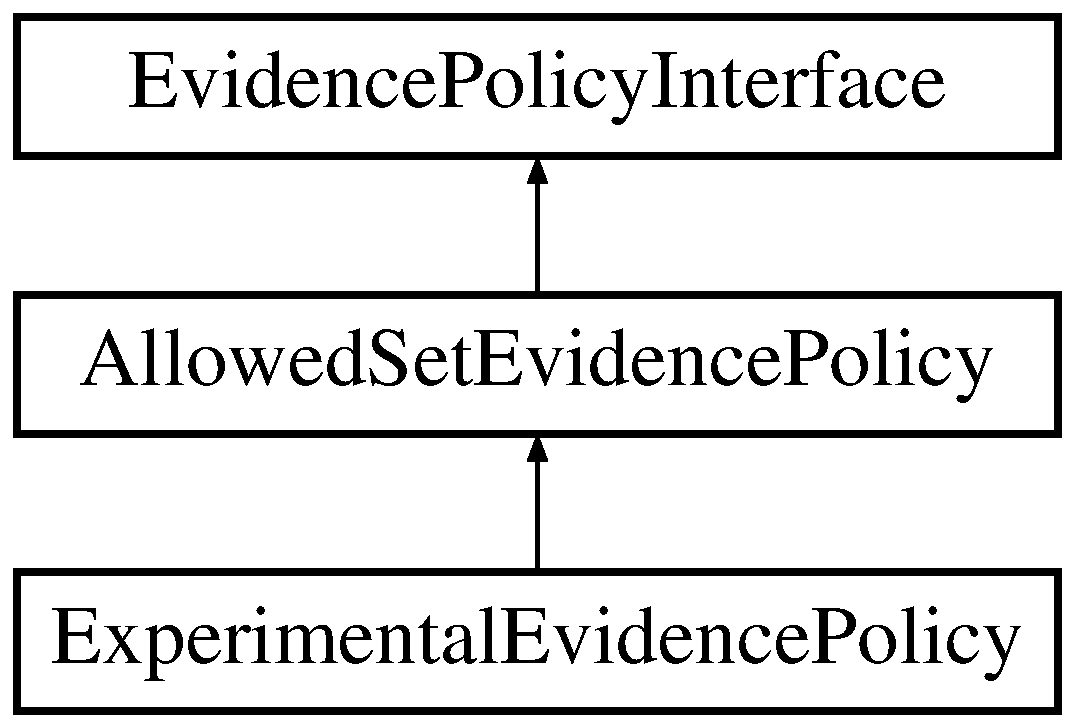
\includegraphics[height=3.000000cm]{classExperimentalEvidencePolicy}
\end{center}
\end{figure}
\subsection*{Public Member Functions}
\begin{DoxyCompactItemize}
\item 
\hyperlink{classExperimentalEvidencePolicy_a842128956f37cc8e5d1cb1c175a6a5a4}{Experimental\+Evidence\+Policy} ()
\begin{DoxyCompactList}\small\item\em A constructor. \end{DoxyCompactList}\end{DoxyCompactItemize}


\subsection{Detailed Description}
A class to allow experimental evidence codes for annotations. 

A class to allow only experimental evidence codes for gene annotations. This class extends the \hyperlink{classAllowedSetEvidencePolicy}{Allowed\+Set\+Evidence\+Policy} and adds the experimental evidence codes to the allowed set. 

\subsection{Constructor \& Destructor Documentation}
\index{Experimental\+Evidence\+Policy@{Experimental\+Evidence\+Policy}!Experimental\+Evidence\+Policy@{Experimental\+Evidence\+Policy}}
\index{Experimental\+Evidence\+Policy@{Experimental\+Evidence\+Policy}!Experimental\+Evidence\+Policy@{Experimental\+Evidence\+Policy}}
\subsubsection[{\texorpdfstring{Experimental\+Evidence\+Policy()}{ExperimentalEvidencePolicy()}}]{\setlength{\rightskip}{0pt plus 5cm}Experimental\+Evidence\+Policy\+::\+Experimental\+Evidence\+Policy (
\begin{DoxyParamCaption}
{}
\end{DoxyParamCaption}
)\hspace{0.3cm}{\ttfamily [inline]}}\hypertarget{classExperimentalEvidencePolicy_a842128956f37cc8e5d1cb1c175a6a5a4}{}\label{classExperimentalEvidencePolicy_a842128956f37cc8e5d1cb1c175a6a5a4}


A constructor. 

Creates the default(empty) \hyperlink{classAllowedSetEvidencePolicy}{Allowed\+Set\+Evidence\+Policy} 

The documentation for this class was generated from the following file\+:\begin{DoxyCompactItemize}
\item 
ggtk/Experimental\+Evidence\+Policy.\+hpp\end{DoxyCompactItemize}

\hypertarget{classFrontierSharedInformation}{}\section{Frontier\+Shared\+Information Class Reference}
\label{classFrontierSharedInformation}\index{Frontier\+Shared\+Information@{Frontier\+Shared\+Information}}


A class to calculate shared infromation across disjoint common ancestors in linear time.  




{\ttfamily \#include $<$ggtk/\+Frontier\+Shared\+Information.\+hpp$>$}

Inheritance diagram for Frontier\+Shared\+Information\+:\begin{figure}[H]
\begin{center}
\leavevmode
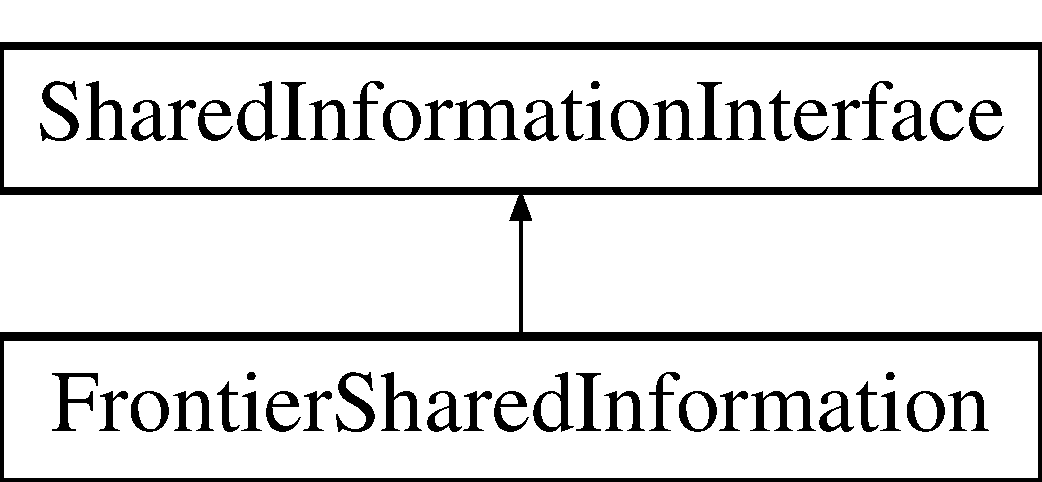
\includegraphics[height=2.000000cm]{classFrontierSharedInformation}
\end{center}
\end{figure}
\subsection*{Public Member Functions}
\begin{DoxyCompactItemize}
\item 
\hyperlink{classFrontierSharedInformation_afd55b315f784ea9991adaa5320108891}{Frontier\+Shared\+Information} (\hyperlink{classGoGraph}{Go\+Graph} $\ast$go\+Graph, \hyperlink{classTermInformationContentMap}{Term\+Information\+Content\+Map} \&ic\+Map)
\begin{DoxyCompactList}\small\item\em A constructor. \end{DoxyCompactList}\item 
boost\+::unordered\+\_\+set$<$ std\+::string $>$ \hyperlink{classFrontierSharedInformation_a4c9a919ae92d7628bbb5c58ab06c19aa}{get\+Common\+Disjoint\+Ancestors} (const std\+::string \&term\+C1, const std\+::string \&term\+C2)
\begin{DoxyCompactList}\small\item\em A method for determining the common disjunctive ancestors. \end{DoxyCompactList}\item 
double \hyperlink{classFrontierSharedInformation_afd0bf3ea7bb9f4f05f89cc2597bc2dcf}{shared\+Information} (const std\+::string \&termA, const std\+::string \&termB)
\begin{DoxyCompactList}\small\item\em An method for returning the shared information of two terms. \end{DoxyCompactList}\item 
double \hyperlink{classFrontierSharedInformation_a7d9c15e312667dc5ac2af1c7e36f735b}{shared\+Information} (const std\+::string \&term)
\begin{DoxyCompactList}\small\item\em An interface method for returning the shared information of a single terms,or information content. \end{DoxyCompactList}\item 
double \hyperlink{classFrontierSharedInformation_a8301888fc7343848a9ee307849e49125}{max\+Information\+Content} (const std\+::string \&term)
\begin{DoxyCompactList}\small\item\em An interface method for returning the maximum information content for a term. \end{DoxyCompactList}\item 
bool \hyperlink{classFrontierSharedInformation_a4cd9a78345443bdd8c43e7fcee01f9b4}{has\+Term} (const std\+::string \&term)
\begin{DoxyCompactList}\small\item\em An interface method for determining if a term can be found. \end{DoxyCompactList}\item 
bool \hyperlink{classFrontierSharedInformation_a545b12efcab4551d031fb6125f615080}{is\+Same\+Ontology} (const std\+::string \&termA, const std\+::string \&termB)
\begin{DoxyCompactList}\small\item\em An interface method for determining if the two terms are of like ontologies. \end{DoxyCompactList}\end{DoxyCompactItemize}


\subsection{Detailed Description}
A class to calculate shared infromation across disjoint common ancestors in linear time. 

This class calculates shared infromation along a semantic frontier between terms. 

\subsection{Constructor \& Destructor Documentation}
\index{Frontier\+Shared\+Information@{Frontier\+Shared\+Information}!Frontier\+Shared\+Information@{Frontier\+Shared\+Information}}
\index{Frontier\+Shared\+Information@{Frontier\+Shared\+Information}!Frontier\+Shared\+Information@{Frontier\+Shared\+Information}}
\subsubsection[{\texorpdfstring{Frontier\+Shared\+Information(\+Go\+Graph $\ast$go\+Graph, Term\+Information\+Content\+Map \&ic\+Map)}{FrontierSharedInformation(GoGraph *goGraph, TermInformationContentMap &icMap)}}]{\setlength{\rightskip}{0pt plus 5cm}Frontier\+Shared\+Information\+::\+Frontier\+Shared\+Information (
\begin{DoxyParamCaption}
\item[{{\bf Go\+Graph} $\ast$}]{go\+Graph, }
\item[{{\bf Term\+Information\+Content\+Map} \&}]{ic\+Map}
\end{DoxyParamCaption}
)\hspace{0.3cm}{\ttfamily [inline]}}\hypertarget{classFrontierSharedInformation_afd55b315f784ea9991adaa5320108891}{}\label{classFrontierSharedInformation_afd55b315f784ea9991adaa5320108891}


A constructor. 

Creates the \hyperlink{classCoutoGraSMSharedInformation}{Couto\+Gra\+S\+M\+Shared\+Information} class 

\subsection{Member Function Documentation}
\index{Frontier\+Shared\+Information@{Frontier\+Shared\+Information}!get\+Common\+Disjoint\+Ancestors@{get\+Common\+Disjoint\+Ancestors}}
\index{get\+Common\+Disjoint\+Ancestors@{get\+Common\+Disjoint\+Ancestors}!Frontier\+Shared\+Information@{Frontier\+Shared\+Information}}
\subsubsection[{\texorpdfstring{get\+Common\+Disjoint\+Ancestors(const std\+::string \&term\+C1, const std\+::string \&term\+C2)}{getCommonDisjointAncestors(const std::string &termC1, const std::string &termC2)}}]{\setlength{\rightskip}{0pt plus 5cm}boost\+::unordered\+\_\+set$<$std\+::string$>$ Frontier\+Shared\+Information\+::get\+Common\+Disjoint\+Ancestors (
\begin{DoxyParamCaption}
\item[{const std\+::string \&}]{term\+C1, }
\item[{const std\+::string \&}]{term\+C2}
\end{DoxyParamCaption}
)\hspace{0.3cm}{\ttfamily [inline]}}\hypertarget{classFrontierSharedInformation_a4c9a919ae92d7628bbb5c58ab06c19aa}{}\label{classFrontierSharedInformation_a4c9a919ae92d7628bbb5c58ab06c19aa}


A method for determining the common disjunctive ancestors. 

This method returns the common disjunctive ancestors for two terms \index{Frontier\+Shared\+Information@{Frontier\+Shared\+Information}!has\+Term@{has\+Term}}
\index{has\+Term@{has\+Term}!Frontier\+Shared\+Information@{Frontier\+Shared\+Information}}
\subsubsection[{\texorpdfstring{has\+Term(const std\+::string \&term)}{hasTerm(const std::string &term)}}]{\setlength{\rightskip}{0pt plus 5cm}bool Frontier\+Shared\+Information\+::has\+Term (
\begin{DoxyParamCaption}
\item[{const std\+::string \&}]{term}
\end{DoxyParamCaption}
)\hspace{0.3cm}{\ttfamily [inline]}, {\ttfamily [virtual]}}\hypertarget{classFrontierSharedInformation_a4cd9a78345443bdd8c43e7fcee01f9b4}{}\label{classFrontierSharedInformation_a4cd9a78345443bdd8c43e7fcee01f9b4}


An interface method for determining if a term can be found. 

Determines if the term can be found in the current map. 

Implements \hyperlink{classSharedInformationInterface_a3f056cf6a40eea8c1669108087dcd5c8}{Shared\+Information\+Interface}.

\index{Frontier\+Shared\+Information@{Frontier\+Shared\+Information}!is\+Same\+Ontology@{is\+Same\+Ontology}}
\index{is\+Same\+Ontology@{is\+Same\+Ontology}!Frontier\+Shared\+Information@{Frontier\+Shared\+Information}}
\subsubsection[{\texorpdfstring{is\+Same\+Ontology(const std\+::string \&term\+A, const std\+::string \&term\+B)}{isSameOntology(const std::string &termA, const std::string &termB)}}]{\setlength{\rightskip}{0pt plus 5cm}bool Frontier\+Shared\+Information\+::is\+Same\+Ontology (
\begin{DoxyParamCaption}
\item[{const std\+::string \&}]{termA, }
\item[{const std\+::string \&}]{termB}
\end{DoxyParamCaption}
)\hspace{0.3cm}{\ttfamily [inline]}, {\ttfamily [virtual]}}\hypertarget{classFrontierSharedInformation_a545b12efcab4551d031fb6125f615080}{}\label{classFrontierSharedInformation_a545b12efcab4551d031fb6125f615080}


An interface method for determining if the two terms are of like ontologies. 

Determine if two terms are of the same ontology. 

Implements \hyperlink{classSharedInformationInterface_a607463b9736df9c4b8ec3ba9fe41c19d}{Shared\+Information\+Interface}.

\index{Frontier\+Shared\+Information@{Frontier\+Shared\+Information}!max\+Information\+Content@{max\+Information\+Content}}
\index{max\+Information\+Content@{max\+Information\+Content}!Frontier\+Shared\+Information@{Frontier\+Shared\+Information}}
\subsubsection[{\texorpdfstring{max\+Information\+Content(const std\+::string \&term)}{maxInformationContent(const std::string &term)}}]{\setlength{\rightskip}{0pt plus 5cm}double Frontier\+Shared\+Information\+::max\+Information\+Content (
\begin{DoxyParamCaption}
\item[{const std\+::string \&}]{term}
\end{DoxyParamCaption}
)\hspace{0.3cm}{\ttfamily [inline]}, {\ttfamily [virtual]}}\hypertarget{classFrontierSharedInformation_a8301888fc7343848a9ee307849e49125}{}\label{classFrontierSharedInformation_a8301888fc7343848a9ee307849e49125}


An interface method for returning the maximum information content for a term. 

This method provides the absolute max information content within a corpus for normalization purposes. 

Implements \hyperlink{classSharedInformationInterface_a7356ba99509458777972ce0f00ebd999}{Shared\+Information\+Interface}.

\index{Frontier\+Shared\+Information@{Frontier\+Shared\+Information}!shared\+Information@{shared\+Information}}
\index{shared\+Information@{shared\+Information}!Frontier\+Shared\+Information@{Frontier\+Shared\+Information}}
\subsubsection[{\texorpdfstring{shared\+Information(const std\+::string \&term\+A, const std\+::string \&term\+B)}{sharedInformation(const std::string &termA, const std::string &termB)}}]{\setlength{\rightskip}{0pt plus 5cm}double Frontier\+Shared\+Information\+::shared\+Information (
\begin{DoxyParamCaption}
\item[{const std\+::string \&}]{termA, }
\item[{const std\+::string \&}]{termB}
\end{DoxyParamCaption}
)\hspace{0.3cm}{\ttfamily [inline]}, {\ttfamily [virtual]}}\hypertarget{classFrontierSharedInformation_afd0bf3ea7bb9f4f05f89cc2597bc2dcf}{}\label{classFrontierSharedInformation_afd0bf3ea7bb9f4f05f89cc2597bc2dcf}


An method for returning the shared information of two terms. 

This method returns the mean information content of the frontier ancestors 

Implements \hyperlink{classSharedInformationInterface_a76e8858eb598442b86b0fd3be1c519e7}{Shared\+Information\+Interface}.

\index{Frontier\+Shared\+Information@{Frontier\+Shared\+Information}!shared\+Information@{shared\+Information}}
\index{shared\+Information@{shared\+Information}!Frontier\+Shared\+Information@{Frontier\+Shared\+Information}}
\subsubsection[{\texorpdfstring{shared\+Information(const std\+::string \&term)}{sharedInformation(const std::string &term)}}]{\setlength{\rightskip}{0pt plus 5cm}double Frontier\+Shared\+Information\+::shared\+Information (
\begin{DoxyParamCaption}
\item[{const std\+::string \&}]{term}
\end{DoxyParamCaption}
)\hspace{0.3cm}{\ttfamily [inline]}, {\ttfamily [virtual]}}\hypertarget{classFrontierSharedInformation_a7d9c15e312667dc5ac2af1c7e36f735b}{}\label{classFrontierSharedInformation_a7d9c15e312667dc5ac2af1c7e36f735b}


An interface method for returning the shared information of a single terms,or information content. 

This method privdes a mechanism for returing a term\textquotesingle{}s infromation content. 

Implements \hyperlink{classSharedInformationInterface_aba102c0e44fbc098baef6074f1eb37b6}{Shared\+Information\+Interface}.



The documentation for this class was generated from the following file\+:\begin{DoxyCompactItemize}
\item 
ggtk/Frontier\+Shared\+Information.\+hpp\end{DoxyCompactItemize}

\hypertarget{classGafAnnotationParser}{}\section{Gaf\+Annotation\+Parser Class Reference}
\label{classGafAnnotationParser}\index{Gaf\+Annotation\+Parser@{Gaf\+Annotation\+Parser}}


A class to parse a \hyperlink{namespaceGO}{GO} Annotation File (G\+AF, Format 2.\+0).  




{\ttfamily \#include $<$ggtk/\+Gaf\+Annotation\+Parser.\+hpp$>$}

Inheritance diagram for Gaf\+Annotation\+Parser\+:\begin{figure}[H]
\begin{center}
\leavevmode
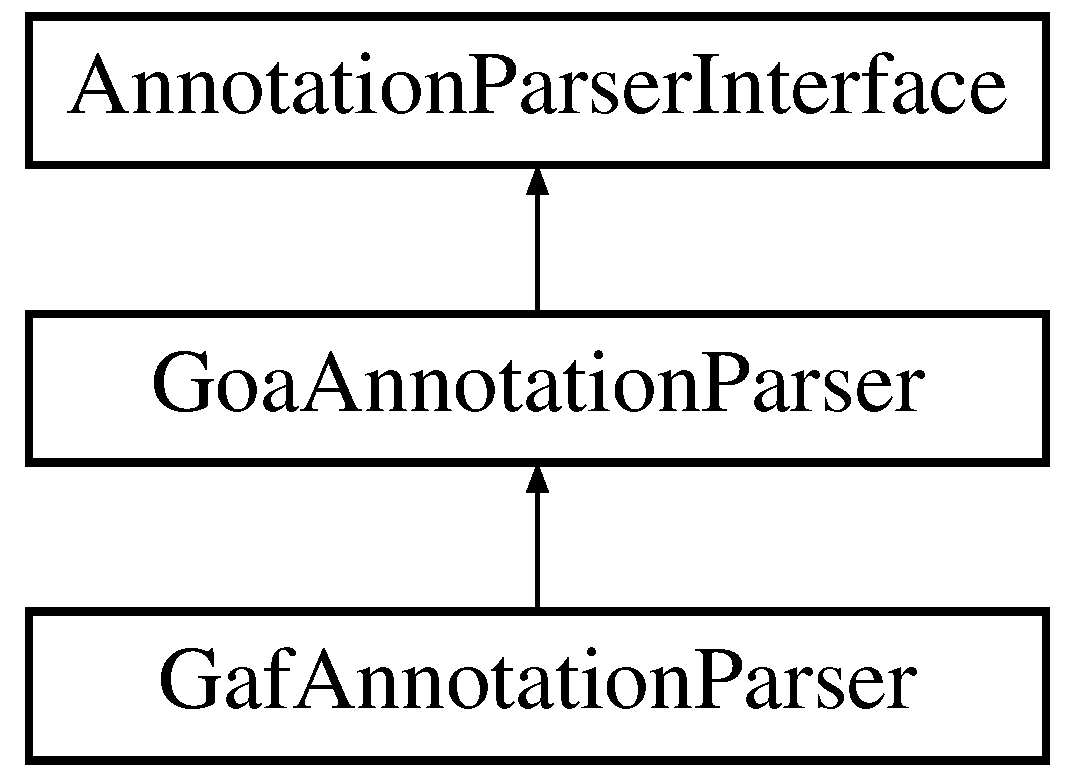
\includegraphics[height=3.000000cm]{classGafAnnotationParser}
\end{center}
\end{figure}
\subsection*{Public Member Functions}
\begin{DoxyCompactItemize}
\item 
\hyperlink{classGafAnnotationParser_a1ec096680cb5e3c4f1111b53cc12ce88}{Gaf\+Annotation\+Parser} ()
\begin{DoxyCompactList}\small\item\em A default constructor method for creating the parser. \end{DoxyCompactList}\item 
\hyperlink{classGafAnnotationParser_a24dc9179f8df7e913c648ea90f60e3b2}{Gaf\+Annotation\+Parser} (\hyperlink{classEvidencePolicyInterface}{Evidence\+Policy\+Interface} $\ast$policy)
\begin{DoxyCompactList}\small\item\em A parameterized constructor method for creating the parser with a policy. \end{DoxyCompactList}\end{DoxyCompactItemize}


\subsection{Detailed Description}
A class to parse a \hyperlink{namespaceGO}{GO} Annotation File (G\+AF, Format 2.\+0). 

This class will read a G\+AF file and return an \hyperlink{classAnnotationData}{Annotation\+Data} object pointer. Defined at\+: \href{http://geneontology.org/page/go-annotation-file-format-20}{\tt http\+://geneontology.\+org/page/go-\/annotation-\/file-\/format-\/20}

Implements \hyperlink{classAnnotationParserInterface}{Annotation\+Parser\+Interface}.

For now, the important aspects of the G\+AF file and G\+OA file are the same. The \hyperlink{classGafAnnotationParser}{Gaf\+Annotation\+Parser} inherits all functionality from \hyperlink{classGoaAnnotationParser}{Goa\+Annotation\+Parser}. This may change in the future. 

\subsection{Constructor \& Destructor Documentation}
\index{Gaf\+Annotation\+Parser@{Gaf\+Annotation\+Parser}!Gaf\+Annotation\+Parser@{Gaf\+Annotation\+Parser}}
\index{Gaf\+Annotation\+Parser@{Gaf\+Annotation\+Parser}!Gaf\+Annotation\+Parser@{Gaf\+Annotation\+Parser}}
\subsubsection[{\texorpdfstring{Gaf\+Annotation\+Parser()}{GafAnnotationParser()}}]{\setlength{\rightskip}{0pt plus 5cm}Gaf\+Annotation\+Parser\+::\+Gaf\+Annotation\+Parser (
\begin{DoxyParamCaption}
{}
\end{DoxyParamCaption}
)\hspace{0.3cm}{\ttfamily [inline]}}\hypertarget{classGafAnnotationParser_a1ec096680cb5e3c4f1111b53cc12ce88}{}\label{classGafAnnotationParser_a1ec096680cb5e3c4f1111b53cc12ce88}


A default constructor method for creating the parser. 

Creates the parser \index{Gaf\+Annotation\+Parser@{Gaf\+Annotation\+Parser}!Gaf\+Annotation\+Parser@{Gaf\+Annotation\+Parser}}
\index{Gaf\+Annotation\+Parser@{Gaf\+Annotation\+Parser}!Gaf\+Annotation\+Parser@{Gaf\+Annotation\+Parser}}
\subsubsection[{\texorpdfstring{Gaf\+Annotation\+Parser(\+Evidence\+Policy\+Interface $\ast$policy)}{GafAnnotationParser(EvidencePolicyInterface *policy)}}]{\setlength{\rightskip}{0pt plus 5cm}Gaf\+Annotation\+Parser\+::\+Gaf\+Annotation\+Parser (
\begin{DoxyParamCaption}
\item[{{\bf Evidence\+Policy\+Interface} $\ast$}]{policy}
\end{DoxyParamCaption}
)\hspace{0.3cm}{\ttfamily [inline]}}\hypertarget{classGafAnnotationParser_a24dc9179f8df7e913c648ea90f60e3b2}{}\label{classGafAnnotationParser_a24dc9179f8df7e913c648ea90f60e3b2}


A parameterized constructor method for creating the parser with a policy. 

Creates the parser with a custom policy 

The documentation for this class was generated from the following file\+:\begin{DoxyCompactItemize}
\item 
ggtk/Gaf\+Annotation\+Parser.\+hpp\end{DoxyCompactItemize}

\hypertarget{classGenomicRegion}{}\section{Genomic\+Region Class Reference}
\label{classGenomicRegion}\index{Genomic\+Region@{Genomic\+Region}}


{\ttfamily \#include $<$ggtk/\+Simple\+Region.\+hpp$>$}

Inheritance diagram for Genomic\+Region\+:\begin{figure}[H]
\begin{center}
\leavevmode
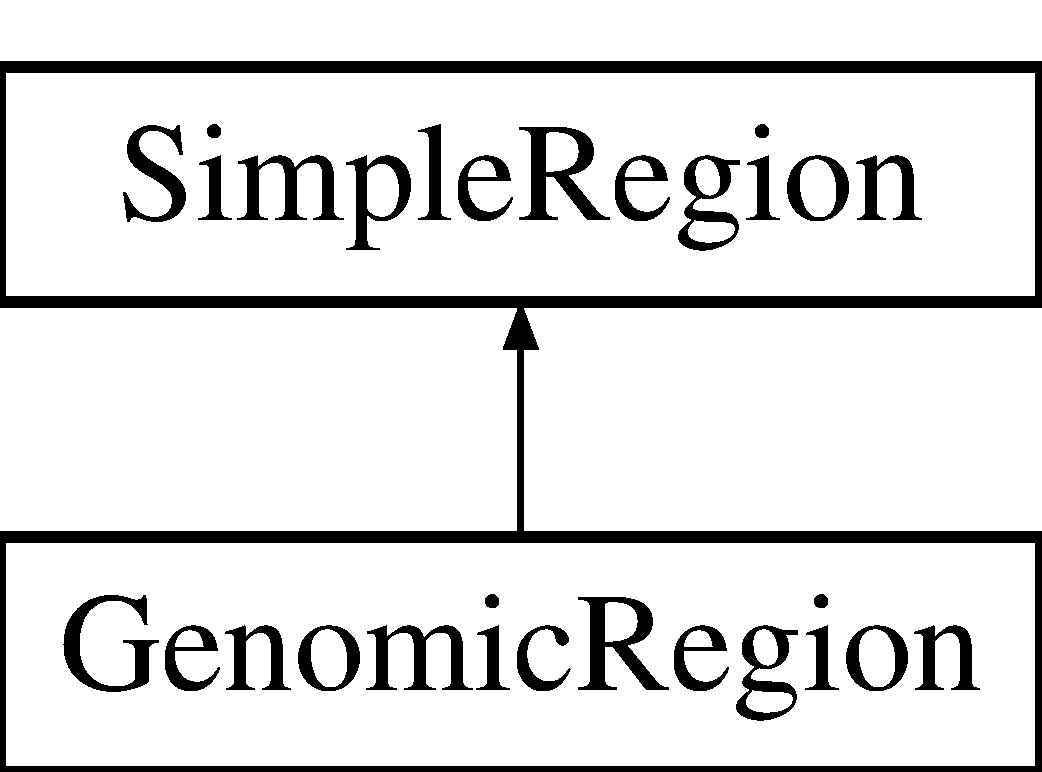
\includegraphics[height=2.000000cm]{classGenomicRegion}
\end{center}
\end{figure}
\subsection*{Public Member Functions}
\begin{DoxyCompactItemize}
\item 
\hyperlink{classGenomicRegion_a48f916f38aad53815e187c28c211a615}{Genomic\+Region} (const std\+::string chrom, const size\+\_\+t start, const size\+\_\+t end, const size\+\_\+t id, std\+::string name, std\+::string desc)
\item 
\hyperlink{classGenomicRegion_a249cece2f76a9085d276ee5970ccfa59}{Genomic\+Region} (const size\+\_\+t id, const size\+\_\+t start, const size\+\_\+t end)
\item 
\hyperlink{classGenomicRegion_a8ff9fe5618b932a1caccbd9072ddaaef}{Genomic\+Region} ()
\item 
std\+::string \hyperlink{classGenomicRegion_af370137d0f3498d1611d85d63571af35}{get\+Chrom} ()
\item 
std\+::string \hyperlink{classGenomicRegion_a206d7c6c224c49b43166b4ad84f1a063}{get\+Name} ()
\item 
std\+::string \hyperlink{classGenomicRegion_a3ce8ecbe3eb5af63e37720aea716ee1f}{get\+Desc} ()
\end{DoxyCompactItemize}
\subsection*{Public Attributes}
\begin{DoxyCompactItemize}
\item 
char \hyperlink{classGenomicRegion_a05a207966ea9e12b3bb580edb0569ab3}{\+\_\+chrom}
\item 
std\+::string \hyperlink{classGenomicRegion_abb827ad33bd08fcf106229c60bc20106}{\+\_\+name}
\item 
std\+::string \hyperlink{classGenomicRegion_af4697f90d465c81be52e9a12f498ca34}{\+\_\+desc}
\end{DoxyCompactItemize}


\subsection{Detailed Description}
E\+X\+P\+E\+R\+I\+M\+E\+N\+T\+AL\+: \hyperlink{classGenomicRegion}{Genomic\+Region} class inheriting from \hyperlink{classSimpleRegion}{Simple\+Region} Adds a few vaibles to \hyperlink{classSimpleRegion}{Simple\+Region} for use in modeling genomic regions. This class is experimental and will be updated at some point in the future. 

\subsection{Constructor \& Destructor Documentation}
\index{Genomic\+Region@{Genomic\+Region}!Genomic\+Region@{Genomic\+Region}}
\index{Genomic\+Region@{Genomic\+Region}!Genomic\+Region@{Genomic\+Region}}
\subsubsection[{\texorpdfstring{Genomic\+Region(const std\+::string chrom, const size\+\_\+t start, const size\+\_\+t end, const size\+\_\+t id, std\+::string name, std\+::string desc)}{GenomicRegion(const std::string chrom, const size_t start, const size_t end, const size_t id, std::string name, std::string desc)}}]{\setlength{\rightskip}{0pt plus 5cm}Genomic\+Region\+::\+Genomic\+Region (
\begin{DoxyParamCaption}
\item[{const std\+::string}]{chrom, }
\item[{const size\+\_\+t}]{start, }
\item[{const size\+\_\+t}]{end, }
\item[{const size\+\_\+t}]{id, }
\item[{std\+::string}]{name, }
\item[{std\+::string}]{desc}
\end{DoxyParamCaption}
)\hspace{0.3cm}{\ttfamily [inline]}}\hypertarget{classGenomicRegion_a48f916f38aad53815e187c28c211a615}{}\label{classGenomicRegion_a48f916f38aad53815e187c28c211a615}
a parameterized constructor for the genomic region. \index{Genomic\+Region@{Genomic\+Region}!Genomic\+Region@{Genomic\+Region}}
\index{Genomic\+Region@{Genomic\+Region}!Genomic\+Region@{Genomic\+Region}}
\subsubsection[{\texorpdfstring{Genomic\+Region(const size\+\_\+t id, const size\+\_\+t start, const size\+\_\+t end)}{GenomicRegion(const size_t id, const size_t start, const size_t end)}}]{\setlength{\rightskip}{0pt plus 5cm}Genomic\+Region\+::\+Genomic\+Region (
\begin{DoxyParamCaption}
\item[{const size\+\_\+t}]{id, }
\item[{const size\+\_\+t}]{start, }
\item[{const size\+\_\+t}]{end}
\end{DoxyParamCaption}
)\hspace{0.3cm}{\ttfamily [inline]}}\hypertarget{classGenomicRegion_a249cece2f76a9085d276ee5970ccfa59}{}\label{classGenomicRegion_a249cece2f76a9085d276ee5970ccfa59}
a simple parametrized constructor for the genomic region \index{Genomic\+Region@{Genomic\+Region}!Genomic\+Region@{Genomic\+Region}}
\index{Genomic\+Region@{Genomic\+Region}!Genomic\+Region@{Genomic\+Region}}
\subsubsection[{\texorpdfstring{Genomic\+Region()}{GenomicRegion()}}]{\setlength{\rightskip}{0pt plus 5cm}Genomic\+Region\+::\+Genomic\+Region (
\begin{DoxyParamCaption}
{}
\end{DoxyParamCaption}
)\hspace{0.3cm}{\ttfamily [inline]}}\hypertarget{classGenomicRegion_a8ff9fe5618b932a1caccbd9072ddaaef}{}\label{classGenomicRegion_a8ff9fe5618b932a1caccbd9072ddaaef}
a default constructor for the genomic region 

\subsection{Member Function Documentation}
\index{Genomic\+Region@{Genomic\+Region}!get\+Chrom@{get\+Chrom}}
\index{get\+Chrom@{get\+Chrom}!Genomic\+Region@{Genomic\+Region}}
\subsubsection[{\texorpdfstring{get\+Chrom()}{getChrom()}}]{\setlength{\rightskip}{0pt plus 5cm}std\+::string Genomic\+Region\+::get\+Chrom (
\begin{DoxyParamCaption}
{}
\end{DoxyParamCaption}
)\hspace{0.3cm}{\ttfamily [inline]}}\hypertarget{classGenomicRegion_af370137d0f3498d1611d85d63571af35}{}\label{classGenomicRegion_af370137d0f3498d1611d85d63571af35}
returns the chromosome for the genomic region \index{Genomic\+Region@{Genomic\+Region}!get\+Desc@{get\+Desc}}
\index{get\+Desc@{get\+Desc}!Genomic\+Region@{Genomic\+Region}}
\subsubsection[{\texorpdfstring{get\+Desc()}{getDesc()}}]{\setlength{\rightskip}{0pt plus 5cm}std\+::string Genomic\+Region\+::get\+Desc (
\begin{DoxyParamCaption}
{}
\end{DoxyParamCaption}
)\hspace{0.3cm}{\ttfamily [inline]}}\hypertarget{classGenomicRegion_a3ce8ecbe3eb5af63e37720aea716ee1f}{}\label{classGenomicRegion_a3ce8ecbe3eb5af63e37720aea716ee1f}
accessor for the genomic region\textquotesingle{}s description \index{Genomic\+Region@{Genomic\+Region}!get\+Name@{get\+Name}}
\index{get\+Name@{get\+Name}!Genomic\+Region@{Genomic\+Region}}
\subsubsection[{\texorpdfstring{get\+Name()}{getName()}}]{\setlength{\rightskip}{0pt plus 5cm}std\+::string Genomic\+Region\+::get\+Name (
\begin{DoxyParamCaption}
{}
\end{DoxyParamCaption}
)\hspace{0.3cm}{\ttfamily [inline]}}\hypertarget{classGenomicRegion_a206d7c6c224c49b43166b4ad84f1a063}{}\label{classGenomicRegion_a206d7c6c224c49b43166b4ad84f1a063}
accessor for the genomic region\textquotesingle{}s name 

\subsection{Member Data Documentation}
\index{Genomic\+Region@{Genomic\+Region}!\+\_\+chrom@{\+\_\+chrom}}
\index{\+\_\+chrom@{\+\_\+chrom}!Genomic\+Region@{Genomic\+Region}}
\subsubsection[{\texorpdfstring{\+\_\+chrom}{_chrom}}]{\setlength{\rightskip}{0pt plus 5cm}char Genomic\+Region\+::\+\_\+chrom}\hypertarget{classGenomicRegion_a05a207966ea9e12b3bb580edb0569ab3}{}\label{classGenomicRegion_a05a207966ea9e12b3bb580edb0569ab3}
a character representing the chromosome \index{Genomic\+Region@{Genomic\+Region}!\+\_\+desc@{\+\_\+desc}}
\index{\+\_\+desc@{\+\_\+desc}!Genomic\+Region@{Genomic\+Region}}
\subsubsection[{\texorpdfstring{\+\_\+desc}{_desc}}]{\setlength{\rightskip}{0pt plus 5cm}std\+::string Genomic\+Region\+::\+\_\+desc}\hypertarget{classGenomicRegion_af4697f90d465c81be52e9a12f498ca34}{}\label{classGenomicRegion_af4697f90d465c81be52e9a12f498ca34}
a description for the region \index{Genomic\+Region@{Genomic\+Region}!\+\_\+name@{\+\_\+name}}
\index{\+\_\+name@{\+\_\+name}!Genomic\+Region@{Genomic\+Region}}
\subsubsection[{\texorpdfstring{\+\_\+name}{_name}}]{\setlength{\rightskip}{0pt plus 5cm}std\+::string Genomic\+Region\+::\+\_\+name}\hypertarget{classGenomicRegion_abb827ad33bd08fcf106229c60bc20106}{}\label{classGenomicRegion_abb827ad33bd08fcf106229c60bc20106}
the name or accession of the region 

The documentation for this class was generated from the following file\+:\begin{DoxyCompactItemize}
\item 
ggtk/Simple\+Region.\+hpp\end{DoxyCompactItemize}

\hypertarget{classGentlemanUISimilarity}{}\section{Gentleman\+U\+I\+Similarity Class Reference}
\label{classGentlemanUISimilarity}\index{Gentleman\+U\+I\+Similarity@{Gentleman\+U\+I\+Similarity}}


A class to calculate Gentleman\textquotesingle{}s UI similarity between go terms for 2 sets.  




{\ttfamily \#include $<$ggtk/\+Gentleman\+Sim\+U\+I\+Set\+Similarity.\+hpp$>$}

Inheritance diagram for Gentleman\+U\+I\+Similarity\+:\begin{figure}[H]
\begin{center}
\leavevmode
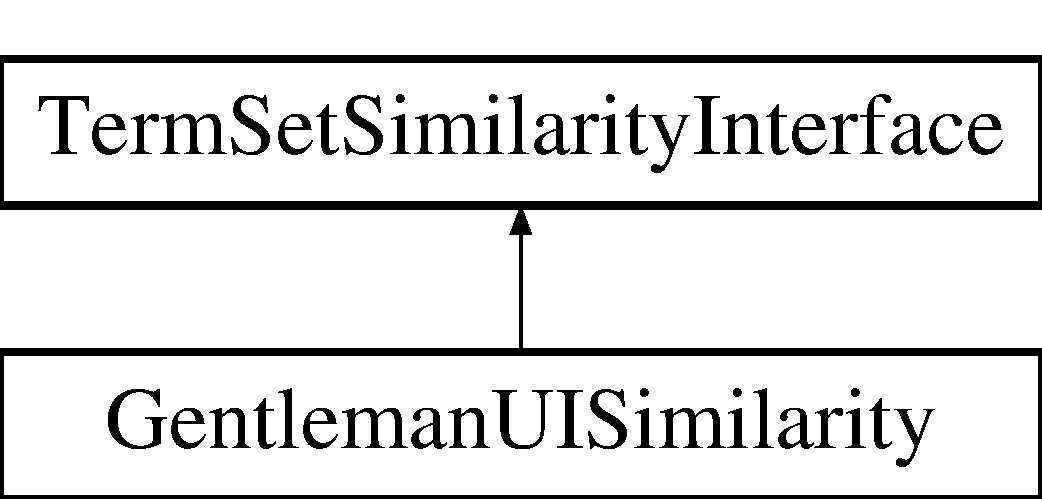
\includegraphics[height=2.000000cm]{classGentlemanUISimilarity}
\end{center}
\end{figure}
\subsection*{Public Member Functions}
\begin{DoxyCompactItemize}
\item 
\hyperlink{classGentlemanUISimilarity_af6e913ef9fc584207a25dc732e6492b0}{Gentleman\+U\+I\+Similarity} (\hyperlink{classTermSimilarityInterface}{Term\+Similarity\+Interface} $\ast$sim\+Measure)
\begin{DoxyCompactList}\small\item\em Constructor. \end{DoxyCompactList}\item 
double \hyperlink{classGentlemanUISimilarity_adc95af100919a4c056ab1a45af09c1ac}{calculate\+Similarity} (boost\+::unordered\+\_\+set$<$ std\+::string $>$ termsA, boost\+::unordered\+\_\+set$<$ std\+::string $>$ termsB)
\begin{DoxyCompactList}\small\item\em A method for calculating term set to term set similarity for \hyperlink{namespaceGO}{GO} terms;. \end{DoxyCompactList}\end{DoxyCompactItemize}


\subsection{Detailed Description}
A class to calculate Gentleman\textquotesingle{}s UI similarity between go terms for 2 sets. 

This is a stub. 

\subsection{Constructor \& Destructor Documentation}
\index{Gentleman\+U\+I\+Similarity@{Gentleman\+U\+I\+Similarity}!Gentleman\+U\+I\+Similarity@{Gentleman\+U\+I\+Similarity}}
\index{Gentleman\+U\+I\+Similarity@{Gentleman\+U\+I\+Similarity}!Gentleman\+U\+I\+Similarity@{Gentleman\+U\+I\+Similarity}}
\subsubsection[{\texorpdfstring{Gentleman\+U\+I\+Similarity(\+Term\+Similarity\+Interface $\ast$sim\+Measure)}{GentlemanUISimilarity(TermSimilarityInterface *simMeasure)}}]{\setlength{\rightskip}{0pt plus 5cm}Gentleman\+U\+I\+Similarity\+::\+Gentleman\+U\+I\+Similarity (
\begin{DoxyParamCaption}
\item[{{\bf Term\+Similarity\+Interface} $\ast$}]{sim\+Measure}
\end{DoxyParamCaption}
)\hspace{0.3cm}{\ttfamily [inline]}}\hypertarget{classGentlemanUISimilarity_af6e913ef9fc584207a25dc732e6492b0}{}\label{classGentlemanUISimilarity_af6e913ef9fc584207a25dc732e6492b0}


Constructor. 

Creates the \hyperlink{classGentlemanUISimilarity}{Gentleman\+U\+I\+Similarity} class assigning the similarity measure private memeber. 

\subsection{Member Function Documentation}
\index{Gentleman\+U\+I\+Similarity@{Gentleman\+U\+I\+Similarity}!calculate\+Similarity@{calculate\+Similarity}}
\index{calculate\+Similarity@{calculate\+Similarity}!Gentleman\+U\+I\+Similarity@{Gentleman\+U\+I\+Similarity}}
\subsubsection[{\texorpdfstring{calculate\+Similarity(boost\+::unordered\+\_\+set$<$ std\+::string $>$ terms\+A, boost\+::unordered\+\_\+set$<$ std\+::string $>$ terms\+B)}{calculateSimilarity(boost::unordered_set< std::string > termsA, boost::unordered_set< std::string > termsB)}}]{\setlength{\rightskip}{0pt plus 5cm}double Gentleman\+U\+I\+Similarity\+::calculate\+Similarity (
\begin{DoxyParamCaption}
\item[{boost\+::unordered\+\_\+set$<$ std\+::string $>$}]{termsA, }
\item[{boost\+::unordered\+\_\+set$<$ std\+::string $>$}]{termsB}
\end{DoxyParamCaption}
)\hspace{0.3cm}{\ttfamily [inline]}}\hypertarget{classGentlemanUISimilarity_adc95af100919a4c056ab1a45af09c1ac}{}\label{classGentlemanUISimilarity_adc95af100919a4c056ab1a45af09c1ac}


A method for calculating term set to term set similarity for \hyperlink{namespaceGO}{GO} terms;. 

This method returns the best match average similarity. 

The documentation for this class was generated from the following file\+:\begin{DoxyCompactItemize}
\item 
ggtk/Gentleman\+Sim\+U\+I\+Set\+Similarity.\+hpp\end{DoxyCompactItemize}

\hypertarget{classGoaAnnotationParser}{}\section{Goa\+Annotation\+Parser Class Reference}
\label{classGoaAnnotationParser}\index{Goa\+Annotation\+Parser@{Goa\+Annotation\+Parser}}


A class to parse a Uniprot Gene Ontolog Annotation (G\+OA) file.  




{\ttfamily \#include $<$ggtk/\+Goa\+Annotation\+Parser.\+hpp$>$}

Inheritance diagram for Goa\+Annotation\+Parser\+:\begin{figure}[H]
\begin{center}
\leavevmode
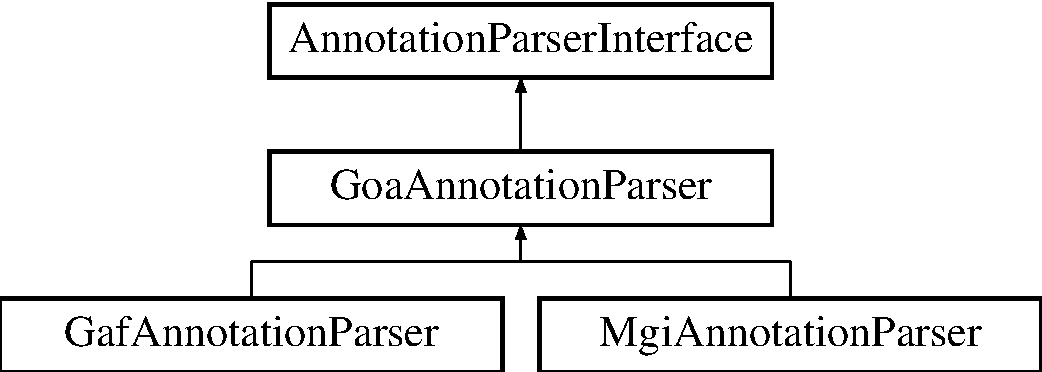
\includegraphics[height=3.000000cm]{classGoaAnnotationParser}
\end{center}
\end{figure}
\subsection*{Public Member Functions}
\begin{DoxyCompactItemize}
\item 
\hyperlink{classAnnotationData}{Annotation\+Data} $\ast$ \hyperlink{classGoaAnnotationParser_a2973e2dcfecea10e09da13ed0ab27dff}{parse\+Annotation\+File} (std\+::string filename)
\begin{DoxyCompactList}\small\item\em An interface method for parsing an annotation file. \end{DoxyCompactList}\item 
bool \hyperlink{classGoaAnnotationParser_aa8093812131c34de52b084ff2b02abbf}{is\+File\+Good} (const std\+::string \&file\+Name)
\begin{DoxyCompactList}\small\item\em A method for checking if a file exists and is formatted correctly. \end{DoxyCompactList}\item 
\hyperlink{classGoaAnnotationParser_a3f415dfbfd2bce5143eef60532ebadea}{Goa\+Annotation\+Parser} (\hyperlink{classEvidencePolicyInterface}{Evidence\+Policy\+Interface} $\ast$policy)
\begin{DoxyCompactList}\small\item\em A parameterized constructor method for creating the parser with a policy. \end{DoxyCompactList}\item 
\hyperlink{classGoaAnnotationParser_aa06b6ba409d97fe794ae1a7606864e65}{Goa\+Annotation\+Parser} ()
\begin{DoxyCompactList}\small\item\em A default constructor method for creating the parser with a policy. \end{DoxyCompactList}\item 
\hyperlink{classAnnotationParserInterface}{Annotation\+Parser\+Interface} $\ast$ \hyperlink{classGoaAnnotationParser_a266297bb5a107572c98515f692684369}{clone} ()
\begin{DoxyCompactList}\small\item\em An interface method for creating a new instance of the parser. \end{DoxyCompactList}\end{DoxyCompactItemize}


\subsection{Detailed Description}
A class to parse a Uniprot Gene Ontolog Annotation (G\+OA) file. 

This class will read a G\+OA file an return an \hyperlink{classAnnotationData}{Annotation\+Data} object pointer. Defined at\+: \href{http://www.ebi.ac.uk/GOA}{\tt http\+://www.\+ebi.\+ac.\+uk/\+G\+OA}

Implements \hyperlink{classAnnotationParserInterface}{Annotation\+Parser\+Interface} 

\subsection{Constructor \& Destructor Documentation}
\index{Goa\+Annotation\+Parser@{Goa\+Annotation\+Parser}!Goa\+Annotation\+Parser@{Goa\+Annotation\+Parser}}
\index{Goa\+Annotation\+Parser@{Goa\+Annotation\+Parser}!Goa\+Annotation\+Parser@{Goa\+Annotation\+Parser}}
\subsubsection[{\texorpdfstring{Goa\+Annotation\+Parser(\+Evidence\+Policy\+Interface $\ast$policy)}{GoaAnnotationParser(EvidencePolicyInterface *policy)}}]{\setlength{\rightskip}{0pt plus 5cm}Goa\+Annotation\+Parser\+::\+Goa\+Annotation\+Parser (
\begin{DoxyParamCaption}
\item[{{\bf Evidence\+Policy\+Interface} $\ast$}]{policy}
\end{DoxyParamCaption}
)\hspace{0.3cm}{\ttfamily [inline]}}\hypertarget{classGoaAnnotationParser_a3f415dfbfd2bce5143eef60532ebadea}{}\label{classGoaAnnotationParser_a3f415dfbfd2bce5143eef60532ebadea}


A parameterized constructor method for creating the parser with a policy. 

Creates the parser \index{Goa\+Annotation\+Parser@{Goa\+Annotation\+Parser}!Goa\+Annotation\+Parser@{Goa\+Annotation\+Parser}}
\index{Goa\+Annotation\+Parser@{Goa\+Annotation\+Parser}!Goa\+Annotation\+Parser@{Goa\+Annotation\+Parser}}
\subsubsection[{\texorpdfstring{Goa\+Annotation\+Parser()}{GoaAnnotationParser()}}]{\setlength{\rightskip}{0pt plus 5cm}Goa\+Annotation\+Parser\+::\+Goa\+Annotation\+Parser (
\begin{DoxyParamCaption}
{}
\end{DoxyParamCaption}
)\hspace{0.3cm}{\ttfamily [inline]}}\hypertarget{classGoaAnnotationParser_aa06b6ba409d97fe794ae1a7606864e65}{}\label{classGoaAnnotationParser_aa06b6ba409d97fe794ae1a7606864e65}


A default constructor method for creating the parser with a policy. 

Creates the parser 

\subsection{Member Function Documentation}
\index{Goa\+Annotation\+Parser@{Goa\+Annotation\+Parser}!clone@{clone}}
\index{clone@{clone}!Goa\+Annotation\+Parser@{Goa\+Annotation\+Parser}}
\subsubsection[{\texorpdfstring{clone()}{clone()}}]{\setlength{\rightskip}{0pt plus 5cm}{\bf Annotation\+Parser\+Interface}$\ast$ Goa\+Annotation\+Parser\+::clone (
\begin{DoxyParamCaption}
{}
\end{DoxyParamCaption}
)\hspace{0.3cm}{\ttfamily [inline]}, {\ttfamily [virtual]}}\hypertarget{classGoaAnnotationParser_a266297bb5a107572c98515f692684369}{}\label{classGoaAnnotationParser_a266297bb5a107572c98515f692684369}


An interface method for creating a new instance of the parser. 

This method returns a new instance of the class. This method partially fulfills the interface contract. 

Implements \hyperlink{classAnnotationParserInterface_a966edeb9aaaa5e94f4c1436afc731a24}{Annotation\+Parser\+Interface}.

\index{Goa\+Annotation\+Parser@{Goa\+Annotation\+Parser}!is\+File\+Good@{is\+File\+Good}}
\index{is\+File\+Good@{is\+File\+Good}!Goa\+Annotation\+Parser@{Goa\+Annotation\+Parser}}
\subsubsection[{\texorpdfstring{is\+File\+Good(const std\+::string \&file\+Name)}{isFileGood(const std::string &fileName)}}]{\setlength{\rightskip}{0pt plus 5cm}bool Goa\+Annotation\+Parser\+::is\+File\+Good (
\begin{DoxyParamCaption}
\item[{const std\+::string \&}]{file\+Name}
\end{DoxyParamCaption}
)\hspace{0.3cm}{\ttfamily [inline]}, {\ttfamily [virtual]}}\hypertarget{classGoaAnnotationParser_aa8093812131c34de52b084ff2b02abbf}{}\label{classGoaAnnotationParser_aa8093812131c34de52b084ff2b02abbf}


A method for checking if a file exists and is formatted correctly. 

This function checks that the file exists and its format can be recognized. 

Implements \hyperlink{classAnnotationParserInterface_a5848b37ca77d78213c87cc5aefebf030}{Annotation\+Parser\+Interface}.

\index{Goa\+Annotation\+Parser@{Goa\+Annotation\+Parser}!parse\+Annotation\+File@{parse\+Annotation\+File}}
\index{parse\+Annotation\+File@{parse\+Annotation\+File}!Goa\+Annotation\+Parser@{Goa\+Annotation\+Parser}}
\subsubsection[{\texorpdfstring{parse\+Annotation\+File(std\+::string filename)}{parseAnnotationFile(std::string filename)}}]{\setlength{\rightskip}{0pt plus 5cm}{\bf Annotation\+Data}$\ast$ Goa\+Annotation\+Parser\+::parse\+Annotation\+File (
\begin{DoxyParamCaption}
\item[{std\+::string}]{filename}
\end{DoxyParamCaption}
)\hspace{0.3cm}{\ttfamily [inline]}, {\ttfamily [virtual]}}\hypertarget{classGoaAnnotationParser_a2973e2dcfecea10e09da13ed0ab27dff}{}\label{classGoaAnnotationParser_a2973e2dcfecea10e09da13ed0ab27dff}


An interface method for parsing an annotation file. 

This method takes a filename as in put and returns a pointer to an \hyperlink{classAnnotationData}{Annotation\+Data} object. This method fulfills part of the interface contract. 

Implements \hyperlink{classAnnotationParserInterface_a1d5cfb902f088a9cf96fdc6b1e5529ab}{Annotation\+Parser\+Interface}.



The documentation for this class was generated from the following file\+:\begin{DoxyCompactItemize}
\item 
ggtk/Goa\+Annotation\+Parser.\+hpp\end{DoxyCompactItemize}

\hypertarget{classGoGraph}{}\section{Go\+Graph Class Reference}
\label{classGoGraph}\index{Go\+Graph@{Go\+Graph}}


This class holds the Gene Ontology directed acyclic graph.  




{\ttfamily \#include $<$ggtk/\+Go\+Graph.\+hpp$>$}

\subsection*{Classes}
\begin{DoxyCompactItemize}
\item 
struct \hyperlink{structGoGraph_1_1EdgeProps}{Edge\+Props}
\begin{DoxyCompactList}\small\item\em An Edge Property object. \end{DoxyCompactList}\item 
struct \hyperlink{structGoGraph_1_1VertexProps}{Vertex\+Props}
\begin{DoxyCompactList}\small\item\em A Vertex Property object. \end{DoxyCompactList}\end{DoxyCompactItemize}
\subsection*{Public Types}
\begin{DoxyCompactItemize}
\item 
typedef boost\+::adjacency\+\_\+list$<$ boost\+::vecS, boost\+::vecS, boost\+::bidirectionalS, boost\+::property$<$ boost\+::vertex\+\_\+index\+\_\+t, size\+\_\+t, \hyperlink{structGoGraph_1_1VertexProps}{Vertex\+Props} $>$, boost\+::property$<$ boost\+::edge\+\_\+index\+\_\+t, size\+\_\+t, \hyperlink{structGoGraph_1_1EdgeProps}{Edge\+Props} $>$ $>$ \hyperlink{classGoGraph_a2586bfc8740625d2d615662ac86f10f9}{Graph\+\_\+t}
\begin{DoxyCompactList}\small\item\em A Graph type representing Go. \end{DoxyCompactList}\item 
typedef boost\+::subgraph$<$ \hyperlink{classGoGraph_a2586bfc8740625d2d615662ac86f10f9}{Graph\+\_\+t} $>$ \hyperlink{classGoGraph_aae4ae00d4785dcee01a514feb768f380}{Graph}
\begin{DoxyCompactList}\small\item\em The main Graph type representing Go. \end{DoxyCompactList}\item 
typedef boost\+::graph\+\_\+traits$<$ \hyperlink{classGoGraph_aae4ae00d4785dcee01a514feb768f380}{Graph} $>$\+::vertex\+\_\+descriptor \hyperlink{classGoGraph_afabec0fb17c98de989e7dd9f3a54e650}{Go\+Vertex}
\begin{DoxyCompactList}\small\item\em A vertex object. \end{DoxyCompactList}\item 
typedef boost\+::graph\+\_\+traits$<$ \hyperlink{classGoGraph_aae4ae00d4785dcee01a514feb768f380}{Graph} $>$\+::edge\+\_\+descriptor \hyperlink{classGoGraph_a6a06a7cf401fba8f03f8f68b54744a75}{Go\+Edge}
\begin{DoxyCompactList}\small\item\em An edge object. \end{DoxyCompactList}\item 
typedef boost\+::graph\+\_\+traits$<$ \hyperlink{classGoGraph_aae4ae00d4785dcee01a514feb768f380}{Graph} $>$\+::vertex\+\_\+iterator \hyperlink{classGoGraph_a1e893efb01d71292881b2fa45c771b79}{Go\+Vertex\+Iterator}
\begin{DoxyCompactList}\small\item\em A vertex iterator. \end{DoxyCompactList}\item 
typedef boost\+::graph\+\_\+traits$<$ \hyperlink{classGoGraph_aae4ae00d4785dcee01a514feb768f380}{Graph} $>$\+::in\+\_\+edge\+\_\+iterator \hyperlink{classGoGraph_a749886e553031dcb52c595989129514d}{In\+Edge\+Iterator}
\begin{DoxyCompactList}\small\item\em An in edge iterator. \end{DoxyCompactList}\item 
typedef boost\+::graph\+\_\+traits$<$ \hyperlink{classGoGraph_aae4ae00d4785dcee01a514feb768f380}{Graph} $>$\+::out\+\_\+edge\+\_\+iterator \hyperlink{classGoGraph_a40291cfa00013cbb9cfb400c1fc92379}{Out\+Edge\+Iterator}
\begin{DoxyCompactList}\small\item\em An out edge iterator. \end{DoxyCompactList}\item 
typedef boost\+::property\+\_\+map$<$ \hyperlink{classGoGraph_aae4ae00d4785dcee01a514feb768f380}{Graph}, boost\+::vertex\+\_\+index\+\_\+t $>$\+::type \hyperlink{classGoGraph_a8a262d8dedc41830e5d4208d4d5e76c3}{Vertex\+Index\+Map}
\begin{DoxyCompactList}\small\item\em A vertex to index map. \end{DoxyCompactList}\item 
typedef boost\+::property\+\_\+map$<$ \hyperlink{classGoGraph_aae4ae00d4785dcee01a514feb768f380}{Graph}, boost\+::edge\+\_\+index\+\_\+t $>$\+::type \hyperlink{classGoGraph_a1fd5f6b3ef1f58a665bbc8e317be9817}{Edge\+Index\+Map}
\begin{DoxyCompactList}\small\item\em An edge to index map. \end{DoxyCompactList}\end{DoxyCompactItemize}
\subsection*{Public Member Functions}
\begin{DoxyCompactItemize}
\item 
\hyperlink{classGoGraph_a48e691ba5998d709d457a949687fccca}{$\sim$\+Go\+Graph} ()
\begin{DoxyCompactList}\small\item\em A destructor. \end{DoxyCompactList}\item 
void \hyperlink{classGoGraph_a41f698c030fec41fe59ade6d1c73721f}{insert\+Term} (const std\+::string \&term\+Id, const std\+::string \&name, const std\+::string \&description, const std\+::string \&ontology)
\begin{DoxyCompactList}\small\item\em Method to insert terms into the graph. \end{DoxyCompactList}\item 
void \hyperlink{classGoGraph_a346fcf36ed71479d529a2db974ba8bc3}{insert\+Relationship} (const std\+::string \&term\+Parent, const std\+::string \&term\+Child, const std\+::string \&relationship)
\begin{DoxyCompactList}\small\item\em Method to insert relationship edges into the graph. \end{DoxyCompactList}\item 
std\+::size\+\_\+t \hyperlink{classGoGraph_a624f621a9c3cd956fb664daf113e3729}{get\+Num\+Vertices} ()
\begin{DoxyCompactList}\small\item\em Helper method to get number of vertices. \end{DoxyCompactList}\item 
std\+::size\+\_\+t \hyperlink{classGoGraph_acafdd8e76e3813e1276798bed2194232}{get\+Num\+Edges} ()
\begin{DoxyCompactList}\small\item\em Helper method to get number of edges. \end{DoxyCompactList}\item 
void \hyperlink{classGoGraph_ad82f8d33a7ecc220ac0d93147dafc061}{init\+Maps} ()
\begin{DoxyCompactList}\small\item\em A method to initialize internal index maps. \end{DoxyCompactList}\item 
\hyperlink{classGoGraph_aae4ae00d4785dcee01a514feb768f380}{Graph} $\ast$ \hyperlink{classGoGraph_a752d7576d649cdc0befa982ca5c3ea98}{get\+Graph} ()
\begin{DoxyCompactList}\small\item\em A method to return the boost graph. \end{DoxyCompactList}\item 
bool \hyperlink{classGoGraph_af8ee7588b17f58717afc13acb0a33435}{has\+Term} (const std\+::string \&term)
\begin{DoxyCompactList}\small\item\em A helper method to test term existence. \end{DoxyCompactList}\item 
size\+\_\+t \hyperlink{classGoGraph_ae7b982d3f564013844d8046e732cef76}{get\+Term\+Index} (const std\+::string \&term)
\begin{DoxyCompactList}\small\item\em A helper method to return the index of the term. \end{DoxyCompactList}\item 
std\+::string \hyperlink{classGoGraph_aa885bffcce6c156769236ca2af9a453e}{get\+Term\+String\+Id\+By\+Index} (std\+::size\+\_\+t index)
\begin{DoxyCompactList}\small\item\em A helper method to return the string id based on the index. \end{DoxyCompactList}\item 
std\+::string \hyperlink{classGoGraph_aa046ee2d278114b6c28f4d5be71b81f0}{get\+Term\+Name\+By\+Index} (std\+::size\+\_\+t index)
\begin{DoxyCompactList}\small\item\em A helper method to return the string name based on the index. \end{DoxyCompactList}\item 
std\+::string \hyperlink{classGoGraph_a175dab9ef8da6c3f06e8f71f21699cf6}{get\+Term\+Name} (std\+::string term)
\begin{DoxyCompactList}\small\item\em A helper method to return the string name based on the go term. \end{DoxyCompactList}\item 
std\+::string \hyperlink{classGoGraph_aed5db44d61c949aed72482ee41438856}{get\+Term\+Description\+By\+Index} (std\+::size\+\_\+t index)
\begin{DoxyCompactList}\small\item\em A helper method to return the string description based on the index. \end{DoxyCompactList}\item 
std\+::string \hyperlink{classGoGraph_abd5d984dd3e1df3d754b1f7e86c487ee}{get\+Term\+Description} (std\+::string term)
\begin{DoxyCompactList}\small\item\em A helper method to return the string description based on the go term. \end{DoxyCompactList}\item 
\hyperlink{classGoGraph_afabec0fb17c98de989e7dd9f3a54e650}{Go\+Vertex} \hyperlink{classGoGraph_a1e8f6565c1cdab44ffbbdcd771246f7c}{get\+Root} ()
\begin{DoxyCompactList}\small\item\em A helper method to return the root of the graph. \end{DoxyCompactList}\item 
\hyperlink{namespaceGO_a5ae335887b5cf40a9ef3045be9247fc3}{G\+O\+::\+Onto} \hyperlink{classGoGraph_a9f4f553098e14270f07e7791cfe65447}{get\+Term\+Ontology} (const std\+::string \&term)
\begin{DoxyCompactList}\small\item\em A helper method to return the ontology of a term by term string. \end{DoxyCompactList}\item 
\hyperlink{namespaceGO_a5ae335887b5cf40a9ef3045be9247fc3}{G\+O\+::\+Onto} \hyperlink{classGoGraph_a0531ffa131c90e9871e280aa5faeaa42}{get\+Term\+Ontology\+By\+Index} (std\+::size\+\_\+t index)
\begin{DoxyCompactList}\small\item\em A helper method to return the ontology of a term by index. \end{DoxyCompactList}\item 
\hyperlink{namespaceGO_a5ae335887b5cf40a9ef3045be9247fc3}{G\+O\+::\+Onto} \hyperlink{classGoGraph_a3ae1998fd4765b2f952290150a7d164b}{get\+Term\+Ontology\+By\+Vertex} (\hyperlink{classGoGraph_afabec0fb17c98de989e7dd9f3a54e650}{Go\+Vertex} vertex)
\begin{DoxyCompactList}\small\item\em A helper method to return the ontology of a term by Go\+Vertex. \end{DoxyCompactList}\item 
std\+::size\+\_\+t \hyperlink{classGoGraph_a524fd1ade5d14d4dc3c900bf82162be6}{get\+Vertex\+Index} (\hyperlink{classGoGraph_afabec0fb17c98de989e7dd9f3a54e650}{Go\+Vertex} vertex)
\begin{DoxyCompactList}\small\item\em A helper method to return the index of a Go\+Vertex. \end{DoxyCompactList}\item 
\hyperlink{classGoGraph_afabec0fb17c98de989e7dd9f3a54e650}{Go\+Vertex} \hyperlink{classGoGraph_a69f38e249704b7e8d9f31a2e3bc03633}{get\+Vertex\+By\+Index} (std\+::size\+\_\+t index)
\begin{DoxyCompactList}\small\item\em A helper method to return the Go\+Vertex for the given index. \end{DoxyCompactList}\item 
\hyperlink{classGoGraph_afabec0fb17c98de989e7dd9f3a54e650}{Go\+Vertex} \hyperlink{classGoGraph_aa66361d5993e6fdf5bd320b6ae15e4bc}{get\+Vertex\+By\+Name} (const std\+::string \&term)
\begin{DoxyCompactList}\small\item\em A helper method to return the Go\+Vertex for the given term. \end{DoxyCompactList}\item 
boost\+::unordered\+\_\+set$<$ std\+::string $>$ \hyperlink{classGoGraph_a0d0a197cc51be0c2f9d0f524a8d66b5e}{get\+Descendant\+Terms} (const std\+::string \&term)
\begin{DoxyCompactList}\small\item\em A helper method to get the desendant terms for a given term. \end{DoxyCompactList}\item 
boost\+::unordered\+\_\+set$<$ std\+::string $>$ \hyperlink{classGoGraph_ae31e1546b740439d44860fa9543c83c2}{get\+Ancestor\+Terms} (const std\+::string \&term)
\begin{DoxyCompactList}\small\item\em A helper method to get the ancestor terms for a given term. \end{DoxyCompactList}\item 
boost\+::unordered\+\_\+set$<$ std\+::string $>$ \hyperlink{classGoGraph_a9907ae6a2960e527f02e7cdf9507aeb1}{get\+Parent\+Terms} (const std\+::string \&term)
\begin{DoxyCompactList}\small\item\em A helper method to get the parent terms for a given term. \end{DoxyCompactList}\item 
boost\+::unordered\+\_\+set$<$ std\+::string $>$ \hyperlink{classGoGraph_ace2ad63bbc6bb2d1dd3e182e6e9c793e}{get\+Child\+Terms} (const std\+::string \&term)
\begin{DoxyCompactList}\small\item\em A helper method to get the child terms for a given term. \end{DoxyCompactList}\item 
boost\+::unordered\+\_\+set$<$ std\+::string $>$ \hyperlink{classGoGraph_ab497e840a1a63b5d25d6a104695a54fb}{get\+All\+Terms} ()
\begin{DoxyCompactList}\small\item\em A helper method to retrieve all terms in the \hyperlink{classGoGraph}{Go\+Graph}. \end{DoxyCompactList}\item 
boost\+::unordered\+\_\+set$<$ std\+::string $>$ \hyperlink{classGoGraph_ad4f45995d5cd7ebe4f0c20d8923db268}{get\+All\+Terms\+BP} ()
\begin{DoxyCompactList}\small\item\em A helper method to retrieve all terms in the \hyperlink{classGoGraph}{Go\+Graph} belonging to the BP ontology. \end{DoxyCompactList}\item 
boost\+::unordered\+\_\+set$<$ std\+::string $>$ \hyperlink{classGoGraph_a9e5592682e5e78c5d45364bf714fd0cf}{get\+All\+Terms\+MF} ()
\begin{DoxyCompactList}\small\item\em A helper method to retrieve all terms in the \hyperlink{classGoGraph}{Go\+Graph} belonging to the MF ontology. \end{DoxyCompactList}\item 
boost\+::unordered\+\_\+set$<$ std\+::string $>$ \hyperlink{classGoGraph_a47246d323ea642a2ffe169fa6da40bcf}{get\+All\+Terms\+CC} ()
\begin{DoxyCompactList}\small\item\em A helper method to retrieve all terms in the \hyperlink{classGoGraph}{Go\+Graph} belonging to the CC ontology. \end{DoxyCompactList}\item 
boost\+::unordered\+\_\+set$<$ std\+::string $>$ \hyperlink{classGoGraph_a1df055e607d7dc4650efedf56b149289}{filter\+Set\+For\+Ontology} (const boost\+::unordered\+\_\+set$<$ std\+::string $>$ \&in\+Set, \hyperlink{namespaceGO_a5ae335887b5cf40a9ef3045be9247fc3}{G\+O\+::\+Onto} onto)
\begin{DoxyCompactList}\small\item\em A helper method to filter out all terms not belonging to a particular ontology. \end{DoxyCompactList}\item 
boost\+::unordered\+\_\+set$<$ std\+::string $>$ \hyperlink{classGoGraph_a083e9fe34636a0e996efd0e9d0d65c3b}{filter\+Set\+For\+Ontology} (const std\+::vector$<$ std\+::string $>$ \&in\+Set, \hyperlink{namespaceGO_a5ae335887b5cf40a9ef3045be9247fc3}{G\+O\+::\+Onto} onto)
\begin{DoxyCompactList}\small\item\em A helper method to filter out all terms not belonging to a particular ontology from a vector. \end{DoxyCompactList}\item 
boost\+::unordered\+\_\+set$<$ std\+::string $>$ \hyperlink{classGoGraph_a42f95a4728eac397fce20d2dcfc8a442}{filter\+Set\+For\+BP} (const std\+::vector$<$ std\+::string $>$ \&in\+Set)
\begin{DoxyCompactList}\small\item\em A helper method to retrun only BP terms from a vector. \end{DoxyCompactList}\item 
boost\+::unordered\+\_\+set$<$ std\+::string $>$ \hyperlink{classGoGraph_ac6e27dbb91d23ea04191abac4c06e401}{filter\+Set\+For\+BP} (const boost\+::unordered\+\_\+set$<$ std\+::string $>$ \&in\+Set)
\begin{DoxyCompactList}\small\item\em A helper method to retrun only BP terms from a set. \end{DoxyCompactList}\item 
boost\+::unordered\+\_\+set$<$ std\+::string $>$ \hyperlink{classGoGraph_a22cedc3faddb0ca598620f2868a46046}{filter\+Set\+For\+MF} (const std\+::vector$<$ std\+::string $>$ \&in\+Set)
\begin{DoxyCompactList}\small\item\em A helper method to retrun only MF terms from a vector. \end{DoxyCompactList}\item 
boost\+::unordered\+\_\+set$<$ std\+::string $>$ \hyperlink{classGoGraph_ac1885e77b0a5f5158e7a94b4404f8c9a}{filter\+Set\+For\+MF} (const boost\+::unordered\+\_\+set$<$ std\+::string $>$ \&in\+Set)
\begin{DoxyCompactList}\small\item\em A helper method to retrun only MF terms from a set. \end{DoxyCompactList}\item 
boost\+::unordered\+\_\+set$<$ std\+::string $>$ \hyperlink{classGoGraph_ad1756e5daeea19ec063b67c2a29594be}{filter\+Set\+For\+CC} (const std\+::vector$<$ std\+::string $>$ \&in\+Set)
\begin{DoxyCompactList}\small\item\em A helper method to retrun only CC terms from a vector. \end{DoxyCompactList}\item 
boost\+::unordered\+\_\+set$<$ std\+::string $>$ \hyperlink{classGoGraph_a23fc2ff15da505fa77536adbd9b7d01b}{filter\+Set\+For\+CC} (const boost\+::unordered\+\_\+set$<$ std\+::string $>$ \&in\+Set)
\begin{DoxyCompactList}\small\item\em A helper method to retrun only CC terms from a set. \end{DoxyCompactList}\item 
boost\+::unordered\+\_\+set$<$ std\+::string $>$ \hyperlink{classGoGraph_abaa3ff8f11463a38fd03241ff17d3e75}{get\+Ontology\+Terms} (\hyperlink{namespaceGO_a5ae335887b5cf40a9ef3045be9247fc3}{G\+O\+::\+Onto} ontology)
\begin{DoxyCompactList}\small\item\em A helper method to return only the terms of the give ontology. \end{DoxyCompactList}\item 
\hyperlink{classGoGraph_aae4ae00d4785dcee01a514feb768f380}{Graph} $\ast$ \hyperlink{classGoGraph_a523911c2ddaff88ea64c8f15a01f9fee}{get\+Induced\+Subgraph2} (const std\+::string \&term\+Id)
\begin{DoxyCompactList}\small\item\em A method to return the induced subgraph of a given term, ancestor graph. \end{DoxyCompactList}\item 
\hyperlink{classGoGraph_aae4ae00d4785dcee01a514feb768f380}{Graph} $\ast$ \hyperlink{classGoGraph_a6ec3b30ab6fbd458b4225ec9532a4e14}{get\+Induced\+Subgraph} (const std\+::string \&term\+Id)
\begin{DoxyCompactList}\small\item\em A method to return the induced subgraph of a given term, ancestor graph. \end{DoxyCompactList}\item 
std\+::size\+\_\+t \hyperlink{classGoGraph_a6ce05821a7dfa86e1fa1de412d2c6cb2}{get\+Num\+Components} ()
\begin{DoxyCompactList}\small\item\em A method to calculate the number of connected components of the graph. \end{DoxyCompactList}\end{DoxyCompactItemize}


\subsection{Detailed Description}
This class holds the Gene Ontology directed acyclic graph. 

This class holds the Gene Ontology as a boost graph. It provides the graph data, as well as other strucutres which make working with the graph easier. 

\subsection{Member Typedef Documentation}
\index{Go\+Graph@{Go\+Graph}!Edge\+Index\+Map@{Edge\+Index\+Map}}
\index{Edge\+Index\+Map@{Edge\+Index\+Map}!Go\+Graph@{Go\+Graph}}
\subsubsection[{\texorpdfstring{Edge\+Index\+Map}{EdgeIndexMap}}]{\setlength{\rightskip}{0pt plus 5cm}typedef boost\+::property\+\_\+map$<${\bf Graph}, boost\+::edge\+\_\+index\+\_\+t $>$\+::type {\bf Go\+Graph\+::\+Edge\+Index\+Map}}\hypertarget{classGoGraph_a1fd5f6b3ef1f58a665bbc8e317be9817}{}\label{classGoGraph_a1fd5f6b3ef1f58a665bbc8e317be9817}


An edge to index map. 

A typedef of the boost property\+\_\+map. Saves typing by using Edge\+Index\+Map. \index{Go\+Graph@{Go\+Graph}!Go\+Edge@{Go\+Edge}}
\index{Go\+Edge@{Go\+Edge}!Go\+Graph@{Go\+Graph}}
\subsubsection[{\texorpdfstring{Go\+Edge}{GoEdge}}]{\setlength{\rightskip}{0pt plus 5cm}typedef boost\+::graph\+\_\+traits$<${\bf Graph}$>$\+::edge\+\_\+descriptor {\bf Go\+Graph\+::\+Go\+Edge}}\hypertarget{classGoGraph_a6a06a7cf401fba8f03f8f68b54744a75}{}\label{classGoGraph_a6a06a7cf401fba8f03f8f68b54744a75}


An edge object. 

A typedef of the boost edge\+\_\+descriptor. Saves typing by using Go\+Edge. \index{Go\+Graph@{Go\+Graph}!Go\+Vertex@{Go\+Vertex}}
\index{Go\+Vertex@{Go\+Vertex}!Go\+Graph@{Go\+Graph}}
\subsubsection[{\texorpdfstring{Go\+Vertex}{GoVertex}}]{\setlength{\rightskip}{0pt plus 5cm}typedef boost\+::graph\+\_\+traits$<${\bf Graph}$>$\+::vertex\+\_\+descriptor {\bf Go\+Graph\+::\+Go\+Vertex}}\hypertarget{classGoGraph_afabec0fb17c98de989e7dd9f3a54e650}{}\label{classGoGraph_afabec0fb17c98de989e7dd9f3a54e650}


A vertex object. 

A typedef of the boost vertex\+\_\+descriptor. Saves typing by using Go\+Vertex. \index{Go\+Graph@{Go\+Graph}!Go\+Vertex\+Iterator@{Go\+Vertex\+Iterator}}
\index{Go\+Vertex\+Iterator@{Go\+Vertex\+Iterator}!Go\+Graph@{Go\+Graph}}
\subsubsection[{\texorpdfstring{Go\+Vertex\+Iterator}{GoVertexIterator}}]{\setlength{\rightskip}{0pt plus 5cm}typedef boost\+::graph\+\_\+traits$<${\bf Graph}$>$\+::vertex\+\_\+iterator {\bf Go\+Graph\+::\+Go\+Vertex\+Iterator}}\hypertarget{classGoGraph_a1e893efb01d71292881b2fa45c771b79}{}\label{classGoGraph_a1e893efb01d71292881b2fa45c771b79}


A vertex iterator. 

A typedef of the boost vertex\+\_\+iterator. Saves typing by using Go\+Vertex\+Iterator. \index{Go\+Graph@{Go\+Graph}!Graph@{Graph}}
\index{Graph@{Graph}!Go\+Graph@{Go\+Graph}}
\subsubsection[{\texorpdfstring{Graph}{Graph}}]{\setlength{\rightskip}{0pt plus 5cm}typedef boost\+::subgraph$<${\bf Graph\+\_\+t}$>$ {\bf Go\+Graph\+::\+Graph}}\hypertarget{classGoGraph_aae4ae00d4785dcee01a514feb768f380}{}\label{classGoGraph_aae4ae00d4785dcee01a514feb768f380}


The main Graph type representing Go. 

This typedef defines the main type as a subgraph of Graph\+\_\+t. This allows the the graph to be divided into subgraphs if needed. Virtually not differnece but can cause problems with some boost constructors such as random graph generators. \index{Go\+Graph@{Go\+Graph}!Graph\+\_\+t@{Graph\+\_\+t}}
\index{Graph\+\_\+t@{Graph\+\_\+t}!Go\+Graph@{Go\+Graph}}
\subsubsection[{\texorpdfstring{Graph\+\_\+t}{Graph_t}}]{\setlength{\rightskip}{0pt plus 5cm}typedef boost\+::adjacency\+\_\+list$<$boost\+::vecS, boost\+::vecS, boost\+::bidirectionalS, boost\+::property$<$ boost\+::vertex\+\_\+index\+\_\+t, size\+\_\+t, {\bf Vertex\+Props}$>$, boost\+::property$<$ boost\+::edge\+\_\+index\+\_\+t, size\+\_\+t, {\bf Edge\+Props}$>$ $>$ {\bf Go\+Graph\+::\+Graph\+\_\+t}}\hypertarget{classGoGraph_a2586bfc8740625d2d615662ac86f10f9}{}\label{classGoGraph_a2586bfc8740625d2d615662ac86f10f9}


A Graph type representing Go. 

This typedef defines a graph type used as the basic go graph. This typedef takes \hyperlink{structGoGraph_1_1VertexProps}{Vertex\+Props} and \hyperlink{structGoGraph_1_1EdgeProps}{Edge\+Props} as templete arguments. \index{Go\+Graph@{Go\+Graph}!In\+Edge\+Iterator@{In\+Edge\+Iterator}}
\index{In\+Edge\+Iterator@{In\+Edge\+Iterator}!Go\+Graph@{Go\+Graph}}
\subsubsection[{\texorpdfstring{In\+Edge\+Iterator}{InEdgeIterator}}]{\setlength{\rightskip}{0pt plus 5cm}typedef boost\+::graph\+\_\+traits$<${\bf Graph}$>$\+::in\+\_\+edge\+\_\+iterator {\bf Go\+Graph\+::\+In\+Edge\+Iterator}}\hypertarget{classGoGraph_a749886e553031dcb52c595989129514d}{}\label{classGoGraph_a749886e553031dcb52c595989129514d}


An in edge iterator. 

A typedef of the boost in\+\_\+edge\+\_\+iterator. Saves typing by using In\+Edge\+Iterator. \index{Go\+Graph@{Go\+Graph}!Out\+Edge\+Iterator@{Out\+Edge\+Iterator}}
\index{Out\+Edge\+Iterator@{Out\+Edge\+Iterator}!Go\+Graph@{Go\+Graph}}
\subsubsection[{\texorpdfstring{Out\+Edge\+Iterator}{OutEdgeIterator}}]{\setlength{\rightskip}{0pt plus 5cm}typedef boost\+::graph\+\_\+traits$<${\bf Graph}$>$\+::out\+\_\+edge\+\_\+iterator {\bf Go\+Graph\+::\+Out\+Edge\+Iterator}}\hypertarget{classGoGraph_a40291cfa00013cbb9cfb400c1fc92379}{}\label{classGoGraph_a40291cfa00013cbb9cfb400c1fc92379}


An out edge iterator. 

A typedef of the boost out\+\_\+edge\+\_\+iterator. Saves typing by using Out\+Edge\+Iterator. \index{Go\+Graph@{Go\+Graph}!Vertex\+Index\+Map@{Vertex\+Index\+Map}}
\index{Vertex\+Index\+Map@{Vertex\+Index\+Map}!Go\+Graph@{Go\+Graph}}
\subsubsection[{\texorpdfstring{Vertex\+Index\+Map}{VertexIndexMap}}]{\setlength{\rightskip}{0pt plus 5cm}typedef boost\+::property\+\_\+map$<${\bf Graph}, boost\+::vertex\+\_\+index\+\_\+t $>$\+::type {\bf Go\+Graph\+::\+Vertex\+Index\+Map}}\hypertarget{classGoGraph_a8a262d8dedc41830e5d4208d4d5e76c3}{}\label{classGoGraph_a8a262d8dedc41830e5d4208d4d5e76c3}


A vertex to index map. 

A typedef of the boost property\+\_\+map. Saves typing by using Vertex\+Index\+Map. 

\subsection{Constructor \& Destructor Documentation}
\index{Go\+Graph@{Go\+Graph}!````~Go\+Graph@{$\sim$\+Go\+Graph}}
\index{````~Go\+Graph@{$\sim$\+Go\+Graph}!Go\+Graph@{Go\+Graph}}
\subsubsection[{\texorpdfstring{$\sim$\+Go\+Graph()}{~GoGraph()}}]{\setlength{\rightskip}{0pt plus 5cm}Go\+Graph\+::$\sim$\+Go\+Graph (
\begin{DoxyParamCaption}
{}
\end{DoxyParamCaption}
)\hspace{0.3cm}{\ttfamily [inline]}}\hypertarget{classGoGraph_a48e691ba5998d709d457a949687fccca}{}\label{classGoGraph_a48e691ba5998d709d457a949687fccca}


A destructor. 

Destroying the graph calls clear on all the containers. Other data should be destroyed when leaving scope. 

\subsection{Member Function Documentation}
\index{Go\+Graph@{Go\+Graph}!filter\+Set\+For\+BP@{filter\+Set\+For\+BP}}
\index{filter\+Set\+For\+BP@{filter\+Set\+For\+BP}!Go\+Graph@{Go\+Graph}}
\subsubsection[{\texorpdfstring{filter\+Set\+For\+B\+P(const std\+::vector$<$ std\+::string $>$ \&in\+Set)}{filterSetForBP(const std::vector< std::string > &inSet)}}]{\setlength{\rightskip}{0pt plus 5cm}boost\+::unordered\+\_\+set$<$std\+::string$>$ Go\+Graph\+::filter\+Set\+For\+BP (
\begin{DoxyParamCaption}
\item[{const std\+::vector$<$ std\+::string $>$ \&}]{in\+Set}
\end{DoxyParamCaption}
)\hspace{0.3cm}{\ttfamily [inline]}}\hypertarget{classGoGraph_a42f95a4728eac397fce20d2dcfc8a442}{}\label{classGoGraph_a42f95a4728eac397fce20d2dcfc8a442}


A helper method to retrun only BP terms from a vector. 

This method returns a filtered set containing only BP terms \index{Go\+Graph@{Go\+Graph}!filter\+Set\+For\+BP@{filter\+Set\+For\+BP}}
\index{filter\+Set\+For\+BP@{filter\+Set\+For\+BP}!Go\+Graph@{Go\+Graph}}
\subsubsection[{\texorpdfstring{filter\+Set\+For\+B\+P(const boost\+::unordered\+\_\+set$<$ std\+::string $>$ \&in\+Set)}{filterSetForBP(const boost::unordered_set< std::string > &inSet)}}]{\setlength{\rightskip}{0pt plus 5cm}boost\+::unordered\+\_\+set$<$std\+::string$>$ Go\+Graph\+::filter\+Set\+For\+BP (
\begin{DoxyParamCaption}
\item[{const boost\+::unordered\+\_\+set$<$ std\+::string $>$ \&}]{in\+Set}
\end{DoxyParamCaption}
)\hspace{0.3cm}{\ttfamily [inline]}}\hypertarget{classGoGraph_ac6e27dbb91d23ea04191abac4c06e401}{}\label{classGoGraph_ac6e27dbb91d23ea04191abac4c06e401}


A helper method to retrun only BP terms from a set. 

This method returns a filtered set containing only BP terms \index{Go\+Graph@{Go\+Graph}!filter\+Set\+For\+CC@{filter\+Set\+For\+CC}}
\index{filter\+Set\+For\+CC@{filter\+Set\+For\+CC}!Go\+Graph@{Go\+Graph}}
\subsubsection[{\texorpdfstring{filter\+Set\+For\+C\+C(const std\+::vector$<$ std\+::string $>$ \&in\+Set)}{filterSetForCC(const std::vector< std::string > &inSet)}}]{\setlength{\rightskip}{0pt plus 5cm}boost\+::unordered\+\_\+set$<$std\+::string$>$ Go\+Graph\+::filter\+Set\+For\+CC (
\begin{DoxyParamCaption}
\item[{const std\+::vector$<$ std\+::string $>$ \&}]{in\+Set}
\end{DoxyParamCaption}
)\hspace{0.3cm}{\ttfamily [inline]}}\hypertarget{classGoGraph_ad1756e5daeea19ec063b67c2a29594be}{}\label{classGoGraph_ad1756e5daeea19ec063b67c2a29594be}


A helper method to retrun only CC terms from a vector. 

This method returns a filtered set containing only CC terms \index{Go\+Graph@{Go\+Graph}!filter\+Set\+For\+CC@{filter\+Set\+For\+CC}}
\index{filter\+Set\+For\+CC@{filter\+Set\+For\+CC}!Go\+Graph@{Go\+Graph}}
\subsubsection[{\texorpdfstring{filter\+Set\+For\+C\+C(const boost\+::unordered\+\_\+set$<$ std\+::string $>$ \&in\+Set)}{filterSetForCC(const boost::unordered_set< std::string > &inSet)}}]{\setlength{\rightskip}{0pt plus 5cm}boost\+::unordered\+\_\+set$<$std\+::string$>$ Go\+Graph\+::filter\+Set\+For\+CC (
\begin{DoxyParamCaption}
\item[{const boost\+::unordered\+\_\+set$<$ std\+::string $>$ \&}]{in\+Set}
\end{DoxyParamCaption}
)\hspace{0.3cm}{\ttfamily [inline]}}\hypertarget{classGoGraph_a23fc2ff15da505fa77536adbd9b7d01b}{}\label{classGoGraph_a23fc2ff15da505fa77536adbd9b7d01b}


A helper method to retrun only CC terms from a set. 

This method returns a filtered set containing only CC terms \index{Go\+Graph@{Go\+Graph}!filter\+Set\+For\+MF@{filter\+Set\+For\+MF}}
\index{filter\+Set\+For\+MF@{filter\+Set\+For\+MF}!Go\+Graph@{Go\+Graph}}
\subsubsection[{\texorpdfstring{filter\+Set\+For\+M\+F(const std\+::vector$<$ std\+::string $>$ \&in\+Set)}{filterSetForMF(const std::vector< std::string > &inSet)}}]{\setlength{\rightskip}{0pt plus 5cm}boost\+::unordered\+\_\+set$<$std\+::string$>$ Go\+Graph\+::filter\+Set\+For\+MF (
\begin{DoxyParamCaption}
\item[{const std\+::vector$<$ std\+::string $>$ \&}]{in\+Set}
\end{DoxyParamCaption}
)\hspace{0.3cm}{\ttfamily [inline]}}\hypertarget{classGoGraph_a22cedc3faddb0ca598620f2868a46046}{}\label{classGoGraph_a22cedc3faddb0ca598620f2868a46046}


A helper method to retrun only MF terms from a vector. 

This method returns a filtered set containing only MF terms \index{Go\+Graph@{Go\+Graph}!filter\+Set\+For\+MF@{filter\+Set\+For\+MF}}
\index{filter\+Set\+For\+MF@{filter\+Set\+For\+MF}!Go\+Graph@{Go\+Graph}}
\subsubsection[{\texorpdfstring{filter\+Set\+For\+M\+F(const boost\+::unordered\+\_\+set$<$ std\+::string $>$ \&in\+Set)}{filterSetForMF(const boost::unordered_set< std::string > &inSet)}}]{\setlength{\rightskip}{0pt plus 5cm}boost\+::unordered\+\_\+set$<$std\+::string$>$ Go\+Graph\+::filter\+Set\+For\+MF (
\begin{DoxyParamCaption}
\item[{const boost\+::unordered\+\_\+set$<$ std\+::string $>$ \&}]{in\+Set}
\end{DoxyParamCaption}
)\hspace{0.3cm}{\ttfamily [inline]}}\hypertarget{classGoGraph_ac1885e77b0a5f5158e7a94b4404f8c9a}{}\label{classGoGraph_ac1885e77b0a5f5158e7a94b4404f8c9a}


A helper method to retrun only MF terms from a set. 

This method returns a filtered set containing only MF terms \index{Go\+Graph@{Go\+Graph}!filter\+Set\+For\+Ontology@{filter\+Set\+For\+Ontology}}
\index{filter\+Set\+For\+Ontology@{filter\+Set\+For\+Ontology}!Go\+Graph@{Go\+Graph}}
\subsubsection[{\texorpdfstring{filter\+Set\+For\+Ontology(const boost\+::unordered\+\_\+set$<$ std\+::string $>$ \&in\+Set, G\+O\+::\+Onto onto)}{filterSetForOntology(const boost::unordered_set< std::string > &inSet, GO::Onto onto)}}]{\setlength{\rightskip}{0pt plus 5cm}boost\+::unordered\+\_\+set$<$std\+::string$>$ Go\+Graph\+::filter\+Set\+For\+Ontology (
\begin{DoxyParamCaption}
\item[{const boost\+::unordered\+\_\+set$<$ std\+::string $>$ \&}]{in\+Set, }
\item[{{\bf G\+O\+::\+Onto}}]{onto}
\end{DoxyParamCaption}
)\hspace{0.3cm}{\ttfamily [inline]}}\hypertarget{classGoGraph_a1df055e607d7dc4650efedf56b149289}{}\label{classGoGraph_a1df055e607d7dc4650efedf56b149289}


A helper method to filter out all terms not belonging to a particular ontology. 

This method returns a filtered set of ontology terms matching the given ontology \index{Go\+Graph@{Go\+Graph}!filter\+Set\+For\+Ontology@{filter\+Set\+For\+Ontology}}
\index{filter\+Set\+For\+Ontology@{filter\+Set\+For\+Ontology}!Go\+Graph@{Go\+Graph}}
\subsubsection[{\texorpdfstring{filter\+Set\+For\+Ontology(const std\+::vector$<$ std\+::string $>$ \&in\+Set, G\+O\+::\+Onto onto)}{filterSetForOntology(const std::vector< std::string > &inSet, GO::Onto onto)}}]{\setlength{\rightskip}{0pt plus 5cm}boost\+::unordered\+\_\+set$<$std\+::string$>$ Go\+Graph\+::filter\+Set\+For\+Ontology (
\begin{DoxyParamCaption}
\item[{const std\+::vector$<$ std\+::string $>$ \&}]{in\+Set, }
\item[{{\bf G\+O\+::\+Onto}}]{onto}
\end{DoxyParamCaption}
)\hspace{0.3cm}{\ttfamily [inline]}}\hypertarget{classGoGraph_a083e9fe34636a0e996efd0e9d0d65c3b}{}\label{classGoGraph_a083e9fe34636a0e996efd0e9d0d65c3b}


A helper method to filter out all terms not belonging to a particular ontology from a vector. 

This method returns a filtered set of ontology terms matching the given ontology \index{Go\+Graph@{Go\+Graph}!get\+All\+Terms@{get\+All\+Terms}}
\index{get\+All\+Terms@{get\+All\+Terms}!Go\+Graph@{Go\+Graph}}
\subsubsection[{\texorpdfstring{get\+All\+Terms()}{getAllTerms()}}]{\setlength{\rightskip}{0pt plus 5cm}boost\+::unordered\+\_\+set$<$std\+::string$>$ Go\+Graph\+::get\+All\+Terms (
\begin{DoxyParamCaption}
{}
\end{DoxyParamCaption}
)\hspace{0.3cm}{\ttfamily [inline]}}\hypertarget{classGoGraph_ab497e840a1a63b5d25d6a104695a54fb}{}\label{classGoGraph_ab497e840a1a63b5d25d6a104695a54fb}


A helper method to retrieve all terms in the \hyperlink{classGoGraph}{Go\+Graph}. 

This method returns a set of term strings \index{Go\+Graph@{Go\+Graph}!get\+All\+Terms\+BP@{get\+All\+Terms\+BP}}
\index{get\+All\+Terms\+BP@{get\+All\+Terms\+BP}!Go\+Graph@{Go\+Graph}}
\subsubsection[{\texorpdfstring{get\+All\+Terms\+B\+P()}{getAllTermsBP()}}]{\setlength{\rightskip}{0pt plus 5cm}boost\+::unordered\+\_\+set$<$std\+::string$>$ Go\+Graph\+::get\+All\+Terms\+BP (
\begin{DoxyParamCaption}
{}
\end{DoxyParamCaption}
)\hspace{0.3cm}{\ttfamily [inline]}}\hypertarget{classGoGraph_ad4f45995d5cd7ebe4f0c20d8923db268}{}\label{classGoGraph_ad4f45995d5cd7ebe4f0c20d8923db268}


A helper method to retrieve all terms in the \hyperlink{classGoGraph}{Go\+Graph} belonging to the BP ontology. 

This method returns a set of BP terms in the graph \index{Go\+Graph@{Go\+Graph}!get\+All\+Terms\+CC@{get\+All\+Terms\+CC}}
\index{get\+All\+Terms\+CC@{get\+All\+Terms\+CC}!Go\+Graph@{Go\+Graph}}
\subsubsection[{\texorpdfstring{get\+All\+Terms\+C\+C()}{getAllTermsCC()}}]{\setlength{\rightskip}{0pt plus 5cm}boost\+::unordered\+\_\+set$<$std\+::string$>$ Go\+Graph\+::get\+All\+Terms\+CC (
\begin{DoxyParamCaption}
{}
\end{DoxyParamCaption}
)\hspace{0.3cm}{\ttfamily [inline]}}\hypertarget{classGoGraph_a47246d323ea642a2ffe169fa6da40bcf}{}\label{classGoGraph_a47246d323ea642a2ffe169fa6da40bcf}


A helper method to retrieve all terms in the \hyperlink{classGoGraph}{Go\+Graph} belonging to the CC ontology. 

This method returns a set of CC terms in the graph \index{Go\+Graph@{Go\+Graph}!get\+All\+Terms\+MF@{get\+All\+Terms\+MF}}
\index{get\+All\+Terms\+MF@{get\+All\+Terms\+MF}!Go\+Graph@{Go\+Graph}}
\subsubsection[{\texorpdfstring{get\+All\+Terms\+M\+F()}{getAllTermsMF()}}]{\setlength{\rightskip}{0pt plus 5cm}boost\+::unordered\+\_\+set$<$std\+::string$>$ Go\+Graph\+::get\+All\+Terms\+MF (
\begin{DoxyParamCaption}
{}
\end{DoxyParamCaption}
)\hspace{0.3cm}{\ttfamily [inline]}}\hypertarget{classGoGraph_a9e5592682e5e78c5d45364bf714fd0cf}{}\label{classGoGraph_a9e5592682e5e78c5d45364bf714fd0cf}


A helper method to retrieve all terms in the \hyperlink{classGoGraph}{Go\+Graph} belonging to the MF ontology. 

This method returns a set of MF terms in the graph \index{Go\+Graph@{Go\+Graph}!get\+Ancestor\+Terms@{get\+Ancestor\+Terms}}
\index{get\+Ancestor\+Terms@{get\+Ancestor\+Terms}!Go\+Graph@{Go\+Graph}}
\subsubsection[{\texorpdfstring{get\+Ancestor\+Terms(const std\+::string \&term)}{getAncestorTerms(const std::string &term)}}]{\setlength{\rightskip}{0pt plus 5cm}boost\+::unordered\+\_\+set$<$std\+::string$>$ Go\+Graph\+::get\+Ancestor\+Terms (
\begin{DoxyParamCaption}
\item[{const std\+::string \&}]{term}
\end{DoxyParamCaption}
)\hspace{0.3cm}{\ttfamily [inline]}}\hypertarget{classGoGraph_ae31e1546b740439d44860fa9543c83c2}{}\label{classGoGraph_ae31e1546b740439d44860fa9543c83c2}


A helper method to get the ancestor terms for a given term. 

This method takes a term and returns a list of ancestor terms. \index{Go\+Graph@{Go\+Graph}!get\+Child\+Terms@{get\+Child\+Terms}}
\index{get\+Child\+Terms@{get\+Child\+Terms}!Go\+Graph@{Go\+Graph}}
\subsubsection[{\texorpdfstring{get\+Child\+Terms(const std\+::string \&term)}{getChildTerms(const std::string &term)}}]{\setlength{\rightskip}{0pt plus 5cm}boost\+::unordered\+\_\+set$<$std\+::string$>$ Go\+Graph\+::get\+Child\+Terms (
\begin{DoxyParamCaption}
\item[{const std\+::string \&}]{term}
\end{DoxyParamCaption}
)\hspace{0.3cm}{\ttfamily [inline]}}\hypertarget{classGoGraph_ace2ad63bbc6bb2d1dd3e182e6e9c793e}{}\label{classGoGraph_ace2ad63bbc6bb2d1dd3e182e6e9c793e}


A helper method to get the child terms for a given term. 

This method takes a term and returns a list of child terms. \index{Go\+Graph@{Go\+Graph}!get\+Descendant\+Terms@{get\+Descendant\+Terms}}
\index{get\+Descendant\+Terms@{get\+Descendant\+Terms}!Go\+Graph@{Go\+Graph}}
\subsubsection[{\texorpdfstring{get\+Descendant\+Terms(const std\+::string \&term)}{getDescendantTerms(const std::string &term)}}]{\setlength{\rightskip}{0pt plus 5cm}boost\+::unordered\+\_\+set$<$std\+::string$>$ Go\+Graph\+::get\+Descendant\+Terms (
\begin{DoxyParamCaption}
\item[{const std\+::string \&}]{term}
\end{DoxyParamCaption}
)\hspace{0.3cm}{\ttfamily [inline]}}\hypertarget{classGoGraph_a0d0a197cc51be0c2f9d0f524a8d66b5e}{}\label{classGoGraph_a0d0a197cc51be0c2f9d0f524a8d66b5e}


A helper method to get the desendant terms for a given term. 

This method takes a term and returns a list of desendant terms. \index{Go\+Graph@{Go\+Graph}!get\+Graph@{get\+Graph}}
\index{get\+Graph@{get\+Graph}!Go\+Graph@{Go\+Graph}}
\subsubsection[{\texorpdfstring{get\+Graph()}{getGraph()}}]{\setlength{\rightskip}{0pt plus 5cm}{\bf Graph}$\ast$ Go\+Graph\+::get\+Graph (
\begin{DoxyParamCaption}
{}
\end{DoxyParamCaption}
)\hspace{0.3cm}{\ttfamily [inline]}}\hypertarget{classGoGraph_a752d7576d649cdc0befa982ca5c3ea98}{}\label{classGoGraph_a752d7576d649cdc0befa982ca5c3ea98}


A method to return the boost graph. 

This method is needed to return the graph to other boost algorithms. As stated by boost, subclasses of adjacency\+\_\+list are not recommended. \href{http://www.boost.org/doc/libs/1_54_0/libs/graph/doc/graph_concepts.html}{\tt http\+://www.\+boost.\+org/doc/libs/1\+\_\+54\+\_\+0/libs/graph/doc/graph\+\_\+concepts.\+html} \index{Go\+Graph@{Go\+Graph}!get\+Induced\+Subgraph@{get\+Induced\+Subgraph}}
\index{get\+Induced\+Subgraph@{get\+Induced\+Subgraph}!Go\+Graph@{Go\+Graph}}
\subsubsection[{\texorpdfstring{get\+Induced\+Subgraph(const std\+::string \&term\+Id)}{getInducedSubgraph(const std::string &termId)}}]{\setlength{\rightskip}{0pt plus 5cm}{\bf Graph}$\ast$ Go\+Graph\+::get\+Induced\+Subgraph (
\begin{DoxyParamCaption}
\item[{const std\+::string \&}]{term\+Id}
\end{DoxyParamCaption}
)\hspace{0.3cm}{\ttfamily [inline]}}\hypertarget{classGoGraph_a6ec3b30ab6fbd458b4225ec9532a4e14}{}\label{classGoGraph_a6ec3b30ab6fbd458b4225ec9532a4e14}


A method to return the induced subgraph of a given term, ancestor graph. 

This method returns a subgraph of the graph induced by traversing the ancestors of the given vertex. \index{Go\+Graph@{Go\+Graph}!get\+Induced\+Subgraph2@{get\+Induced\+Subgraph2}}
\index{get\+Induced\+Subgraph2@{get\+Induced\+Subgraph2}!Go\+Graph@{Go\+Graph}}
\subsubsection[{\texorpdfstring{get\+Induced\+Subgraph2(const std\+::string \&term\+Id)}{getInducedSubgraph2(const std::string &termId)}}]{\setlength{\rightskip}{0pt plus 5cm}{\bf Graph}$\ast$ Go\+Graph\+::get\+Induced\+Subgraph2 (
\begin{DoxyParamCaption}
\item[{const std\+::string \&}]{term\+Id}
\end{DoxyParamCaption}
)\hspace{0.3cm}{\ttfamily [inline]}}\hypertarget{classGoGraph_a523911c2ddaff88ea64c8f15a01f9fee}{}\label{classGoGraph_a523911c2ddaff88ea64c8f15a01f9fee}


A method to return the induced subgraph of a given term, ancestor graph. 

This method returns a subgraph of the graph induced by traversing the ancestors of the given vertex. \index{Go\+Graph@{Go\+Graph}!get\+Num\+Components@{get\+Num\+Components}}
\index{get\+Num\+Components@{get\+Num\+Components}!Go\+Graph@{Go\+Graph}}
\subsubsection[{\texorpdfstring{get\+Num\+Components()}{getNumComponents()}}]{\setlength{\rightskip}{0pt plus 5cm}std\+::size\+\_\+t Go\+Graph\+::get\+Num\+Components (
\begin{DoxyParamCaption}
{}
\end{DoxyParamCaption}
)\hspace{0.3cm}{\ttfamily [inline]}}\hypertarget{classGoGraph_a6ce05821a7dfa86e1fa1de412d2c6cb2}{}\label{classGoGraph_a6ce05821a7dfa86e1fa1de412d2c6cb2}


A method to calculate the number of connected components of the graph. 

This method calculates the number of connected components in the graph. This is used to check if the \hyperlink{namespaceGO}{GO} graph conatains only the 3 sub-\/ontologies. \index{Go\+Graph@{Go\+Graph}!get\+Num\+Edges@{get\+Num\+Edges}}
\index{get\+Num\+Edges@{get\+Num\+Edges}!Go\+Graph@{Go\+Graph}}
\subsubsection[{\texorpdfstring{get\+Num\+Edges()}{getNumEdges()}}]{\setlength{\rightskip}{0pt plus 5cm}std\+::size\+\_\+t Go\+Graph\+::get\+Num\+Edges (
\begin{DoxyParamCaption}
{}
\end{DoxyParamCaption}
)\hspace{0.3cm}{\ttfamily [inline]}}\hypertarget{classGoGraph_acafdd8e76e3813e1276798bed2194232}{}\label{classGoGraph_acafdd8e76e3813e1276798bed2194232}


Helper method to get number of edges. 

This method calls boost num\+\_\+edges on the go graph \index{Go\+Graph@{Go\+Graph}!get\+Num\+Vertices@{get\+Num\+Vertices}}
\index{get\+Num\+Vertices@{get\+Num\+Vertices}!Go\+Graph@{Go\+Graph}}
\subsubsection[{\texorpdfstring{get\+Num\+Vertices()}{getNumVertices()}}]{\setlength{\rightskip}{0pt plus 5cm}std\+::size\+\_\+t Go\+Graph\+::get\+Num\+Vertices (
\begin{DoxyParamCaption}
{}
\end{DoxyParamCaption}
)\hspace{0.3cm}{\ttfamily [inline]}}\hypertarget{classGoGraph_a624f621a9c3cd956fb664daf113e3729}{}\label{classGoGraph_a624f621a9c3cd956fb664daf113e3729}


Helper method to get number of vertices. 

This method calls boost num\+\_\+vertices on the go graph \index{Go\+Graph@{Go\+Graph}!get\+Ontology\+Terms@{get\+Ontology\+Terms}}
\index{get\+Ontology\+Terms@{get\+Ontology\+Terms}!Go\+Graph@{Go\+Graph}}
\subsubsection[{\texorpdfstring{get\+Ontology\+Terms(\+G\+O\+::\+Onto ontology)}{getOntologyTerms(GO::Onto ontology)}}]{\setlength{\rightskip}{0pt plus 5cm}boost\+::unordered\+\_\+set$<$std\+::string$>$ Go\+Graph\+::get\+Ontology\+Terms (
\begin{DoxyParamCaption}
\item[{{\bf G\+O\+::\+Onto}}]{ontology}
\end{DoxyParamCaption}
)\hspace{0.3cm}{\ttfamily [inline]}}\hypertarget{classGoGraph_abaa3ff8f11463a38fd03241ff17d3e75}{}\label{classGoGraph_abaa3ff8f11463a38fd03241ff17d3e75}


A helper method to return only the terms of the give ontology. 

Returns only those terms used that occur for the given ontology. \index{Go\+Graph@{Go\+Graph}!get\+Parent\+Terms@{get\+Parent\+Terms}}
\index{get\+Parent\+Terms@{get\+Parent\+Terms}!Go\+Graph@{Go\+Graph}}
\subsubsection[{\texorpdfstring{get\+Parent\+Terms(const std\+::string \&term)}{getParentTerms(const std::string &term)}}]{\setlength{\rightskip}{0pt plus 5cm}boost\+::unordered\+\_\+set$<$std\+::string$>$ Go\+Graph\+::get\+Parent\+Terms (
\begin{DoxyParamCaption}
\item[{const std\+::string \&}]{term}
\end{DoxyParamCaption}
)\hspace{0.3cm}{\ttfamily [inline]}}\hypertarget{classGoGraph_a9907ae6a2960e527f02e7cdf9507aeb1}{}\label{classGoGraph_a9907ae6a2960e527f02e7cdf9507aeb1}


A helper method to get the parent terms for a given term. 

This method takes a term and returns a list of parent terms (immediate ancestors). \index{Go\+Graph@{Go\+Graph}!get\+Root@{get\+Root}}
\index{get\+Root@{get\+Root}!Go\+Graph@{Go\+Graph}}
\subsubsection[{\texorpdfstring{get\+Root()}{getRoot()}}]{\setlength{\rightskip}{0pt plus 5cm}{\bf Go\+Vertex} Go\+Graph\+::get\+Root (
\begin{DoxyParamCaption}
{}
\end{DoxyParamCaption}
)\hspace{0.3cm}{\ttfamily [inline]}}\hypertarget{classGoGraph_a1e8f6565c1cdab44ffbbdcd771246f7c}{}\label{classGoGraph_a1e8f6565c1cdab44ffbbdcd771246f7c}


A helper method to return the root of the graph. 

This method returns the root vertex or first root vertex of a graph. \index{Go\+Graph@{Go\+Graph}!get\+Term\+Description@{get\+Term\+Description}}
\index{get\+Term\+Description@{get\+Term\+Description}!Go\+Graph@{Go\+Graph}}
\subsubsection[{\texorpdfstring{get\+Term\+Description(std\+::string term)}{getTermDescription(std::string term)}}]{\setlength{\rightskip}{0pt plus 5cm}std\+::string Go\+Graph\+::get\+Term\+Description (
\begin{DoxyParamCaption}
\item[{std\+::string}]{term}
\end{DoxyParamCaption}
)\hspace{0.3cm}{\ttfamily [inline]}}\hypertarget{classGoGraph_abd5d984dd3e1df3d754b1f7e86c487ee}{}\label{classGoGraph_abd5d984dd3e1df3d754b1f7e86c487ee}


A helper method to return the string description based on the go term. 

This method returns the term\textquotesingle{}s description string using the go term. \index{Go\+Graph@{Go\+Graph}!get\+Term\+Description\+By\+Index@{get\+Term\+Description\+By\+Index}}
\index{get\+Term\+Description\+By\+Index@{get\+Term\+Description\+By\+Index}!Go\+Graph@{Go\+Graph}}
\subsubsection[{\texorpdfstring{get\+Term\+Description\+By\+Index(std\+::size\+\_\+t index)}{getTermDescriptionByIndex(std::size_t index)}}]{\setlength{\rightskip}{0pt plus 5cm}std\+::string Go\+Graph\+::get\+Term\+Description\+By\+Index (
\begin{DoxyParamCaption}
\item[{std\+::size\+\_\+t}]{index}
\end{DoxyParamCaption}
)\hspace{0.3cm}{\ttfamily [inline]}}\hypertarget{classGoGraph_aed5db44d61c949aed72482ee41438856}{}\label{classGoGraph_aed5db44d61c949aed72482ee41438856}


A helper method to return the string description based on the index. 

This method returns the term\textquotesingle{}s description string using its index. Used mainly for testing. \index{Go\+Graph@{Go\+Graph}!get\+Term\+Index@{get\+Term\+Index}}
\index{get\+Term\+Index@{get\+Term\+Index}!Go\+Graph@{Go\+Graph}}
\subsubsection[{\texorpdfstring{get\+Term\+Index(const std\+::string \&term)}{getTermIndex(const std::string &term)}}]{\setlength{\rightskip}{0pt plus 5cm}size\+\_\+t Go\+Graph\+::get\+Term\+Index (
\begin{DoxyParamCaption}
\item[{const std\+::string \&}]{term}
\end{DoxyParamCaption}
)\hspace{0.3cm}{\ttfamily [inline]}}\hypertarget{classGoGraph_ae7b982d3f564013844d8046e732cef76}{}\label{classGoGraph_ae7b982d3f564013844d8046e732cef76}


A helper method to return the index of the term. 

This method returns the index of the given term. \index{Go\+Graph@{Go\+Graph}!get\+Term\+Name@{get\+Term\+Name}}
\index{get\+Term\+Name@{get\+Term\+Name}!Go\+Graph@{Go\+Graph}}
\subsubsection[{\texorpdfstring{get\+Term\+Name(std\+::string term)}{getTermName(std::string term)}}]{\setlength{\rightskip}{0pt plus 5cm}std\+::string Go\+Graph\+::get\+Term\+Name (
\begin{DoxyParamCaption}
\item[{std\+::string}]{term}
\end{DoxyParamCaption}
)\hspace{0.3cm}{\ttfamily [inline]}}\hypertarget{classGoGraph_a175dab9ef8da6c3f06e8f71f21699cf6}{}\label{classGoGraph_a175dab9ef8da6c3f06e8f71f21699cf6}


A helper method to return the string name based on the go term. 

This method returns the term\textquotesingle{}s string name using the go term. \index{Go\+Graph@{Go\+Graph}!get\+Term\+Name\+By\+Index@{get\+Term\+Name\+By\+Index}}
\index{get\+Term\+Name\+By\+Index@{get\+Term\+Name\+By\+Index}!Go\+Graph@{Go\+Graph}}
\subsubsection[{\texorpdfstring{get\+Term\+Name\+By\+Index(std\+::size\+\_\+t index)}{getTermNameByIndex(std::size_t index)}}]{\setlength{\rightskip}{0pt plus 5cm}std\+::string Go\+Graph\+::get\+Term\+Name\+By\+Index (
\begin{DoxyParamCaption}
\item[{std\+::size\+\_\+t}]{index}
\end{DoxyParamCaption}
)\hspace{0.3cm}{\ttfamily [inline]}}\hypertarget{classGoGraph_aa046ee2d278114b6c28f4d5be71b81f0}{}\label{classGoGraph_aa046ee2d278114b6c28f4d5be71b81f0}


A helper method to return the string name based on the index. 

This method returns the term\textquotesingle{}s string name using its index. Used mainly for testing. \index{Go\+Graph@{Go\+Graph}!get\+Term\+Ontology@{get\+Term\+Ontology}}
\index{get\+Term\+Ontology@{get\+Term\+Ontology}!Go\+Graph@{Go\+Graph}}
\subsubsection[{\texorpdfstring{get\+Term\+Ontology(const std\+::string \&term)}{getTermOntology(const std::string &term)}}]{\setlength{\rightskip}{0pt plus 5cm}{\bf G\+O\+::\+Onto} Go\+Graph\+::get\+Term\+Ontology (
\begin{DoxyParamCaption}
\item[{const std\+::string \&}]{term}
\end{DoxyParamCaption}
)\hspace{0.3cm}{\ttfamily [inline]}}\hypertarget{classGoGraph_a9f4f553098e14270f07e7791cfe65447}{}\label{classGoGraph_a9f4f553098e14270f07e7791cfe65447}


A helper method to return the ontology of a term by term string. 

This method returns the term\textquotesingle{}s ontoogy taking a string term as an argument \index{Go\+Graph@{Go\+Graph}!get\+Term\+Ontology\+By\+Index@{get\+Term\+Ontology\+By\+Index}}
\index{get\+Term\+Ontology\+By\+Index@{get\+Term\+Ontology\+By\+Index}!Go\+Graph@{Go\+Graph}}
\subsubsection[{\texorpdfstring{get\+Term\+Ontology\+By\+Index(std\+::size\+\_\+t index)}{getTermOntologyByIndex(std::size_t index)}}]{\setlength{\rightskip}{0pt plus 5cm}{\bf G\+O\+::\+Onto} Go\+Graph\+::get\+Term\+Ontology\+By\+Index (
\begin{DoxyParamCaption}
\item[{std\+::size\+\_\+t}]{index}
\end{DoxyParamCaption}
)\hspace{0.3cm}{\ttfamily [inline]}}\hypertarget{classGoGraph_a0531ffa131c90e9871e280aa5faeaa42}{}\label{classGoGraph_a0531ffa131c90e9871e280aa5faeaa42}


A helper method to return the ontology of a term by index. 

This method returns the term\textquotesingle{}s ontoogy taking an index as an argument \index{Go\+Graph@{Go\+Graph}!get\+Term\+Ontology\+By\+Vertex@{get\+Term\+Ontology\+By\+Vertex}}
\index{get\+Term\+Ontology\+By\+Vertex@{get\+Term\+Ontology\+By\+Vertex}!Go\+Graph@{Go\+Graph}}
\subsubsection[{\texorpdfstring{get\+Term\+Ontology\+By\+Vertex(\+Go\+Vertex vertex)}{getTermOntologyByVertex(GoVertex vertex)}}]{\setlength{\rightskip}{0pt plus 5cm}{\bf G\+O\+::\+Onto} Go\+Graph\+::get\+Term\+Ontology\+By\+Vertex (
\begin{DoxyParamCaption}
\item[{{\bf Go\+Vertex}}]{vertex}
\end{DoxyParamCaption}
)\hspace{0.3cm}{\ttfamily [inline]}}\hypertarget{classGoGraph_a3ae1998fd4765b2f952290150a7d164b}{}\label{classGoGraph_a3ae1998fd4765b2f952290150a7d164b}


A helper method to return the ontology of a term by Go\+Vertex. 

This method returns the term\textquotesingle{}s ontoogy taking Go\+Vertex as an argument \index{Go\+Graph@{Go\+Graph}!get\+Term\+String\+Id\+By\+Index@{get\+Term\+String\+Id\+By\+Index}}
\index{get\+Term\+String\+Id\+By\+Index@{get\+Term\+String\+Id\+By\+Index}!Go\+Graph@{Go\+Graph}}
\subsubsection[{\texorpdfstring{get\+Term\+String\+Id\+By\+Index(std\+::size\+\_\+t index)}{getTermStringIdByIndex(std::size_t index)}}]{\setlength{\rightskip}{0pt plus 5cm}std\+::string Go\+Graph\+::get\+Term\+String\+Id\+By\+Index (
\begin{DoxyParamCaption}
\item[{std\+::size\+\_\+t}]{index}
\end{DoxyParamCaption}
)\hspace{0.3cm}{\ttfamily [inline]}}\hypertarget{classGoGraph_aa885bffcce6c156769236ca2af9a453e}{}\label{classGoGraph_aa885bffcce6c156769236ca2af9a453e}


A helper method to return the string id based on the index. 

This method returns the term\textquotesingle{}s string id using its index. Used mainly for testing. \index{Go\+Graph@{Go\+Graph}!get\+Vertex\+By\+Index@{get\+Vertex\+By\+Index}}
\index{get\+Vertex\+By\+Index@{get\+Vertex\+By\+Index}!Go\+Graph@{Go\+Graph}}
\subsubsection[{\texorpdfstring{get\+Vertex\+By\+Index(std\+::size\+\_\+t index)}{getVertexByIndex(std::size_t index)}}]{\setlength{\rightskip}{0pt plus 5cm}{\bf Go\+Vertex} Go\+Graph\+::get\+Vertex\+By\+Index (
\begin{DoxyParamCaption}
\item[{std\+::size\+\_\+t}]{index}
\end{DoxyParamCaption}
)\hspace{0.3cm}{\ttfamily [inline]}}\hypertarget{classGoGraph_a69f38e249704b7e8d9f31a2e3bc03633}{}\label{classGoGraph_a69f38e249704b7e8d9f31a2e3bc03633}


A helper method to return the Go\+Vertex for the given index. 

This method returns the Go\+Vertex based on the given index \index{Go\+Graph@{Go\+Graph}!get\+Vertex\+By\+Name@{get\+Vertex\+By\+Name}}
\index{get\+Vertex\+By\+Name@{get\+Vertex\+By\+Name}!Go\+Graph@{Go\+Graph}}
\subsubsection[{\texorpdfstring{get\+Vertex\+By\+Name(const std\+::string \&term)}{getVertexByName(const std::string &term)}}]{\setlength{\rightskip}{0pt plus 5cm}{\bf Go\+Vertex} Go\+Graph\+::get\+Vertex\+By\+Name (
\begin{DoxyParamCaption}
\item[{const std\+::string \&}]{term}
\end{DoxyParamCaption}
)\hspace{0.3cm}{\ttfamily [inline]}}\hypertarget{classGoGraph_aa66361d5993e6fdf5bd320b6ae15e4bc}{}\label{classGoGraph_aa66361d5993e6fdf5bd320b6ae15e4bc}


A helper method to return the Go\+Vertex for the given term. 

This method returns the Go\+Vertex based on the given term \index{Go\+Graph@{Go\+Graph}!get\+Vertex\+Index@{get\+Vertex\+Index}}
\index{get\+Vertex\+Index@{get\+Vertex\+Index}!Go\+Graph@{Go\+Graph}}
\subsubsection[{\texorpdfstring{get\+Vertex\+Index(\+Go\+Vertex vertex)}{getVertexIndex(GoVertex vertex)}}]{\setlength{\rightskip}{0pt plus 5cm}std\+::size\+\_\+t Go\+Graph\+::get\+Vertex\+Index (
\begin{DoxyParamCaption}
\item[{{\bf Go\+Vertex}}]{vertex}
\end{DoxyParamCaption}
)\hspace{0.3cm}{\ttfamily [inline]}}\hypertarget{classGoGraph_a524fd1ade5d14d4dc3c900bf82162be6}{}\label{classGoGraph_a524fd1ade5d14d4dc3c900bf82162be6}


A helper method to return the index of a Go\+Vertex. 

This method returns the index of a Go\+Vertex \index{Go\+Graph@{Go\+Graph}!has\+Term@{has\+Term}}
\index{has\+Term@{has\+Term}!Go\+Graph@{Go\+Graph}}
\subsubsection[{\texorpdfstring{has\+Term(const std\+::string \&term)}{hasTerm(const std::string &term)}}]{\setlength{\rightskip}{0pt plus 5cm}bool Go\+Graph\+::has\+Term (
\begin{DoxyParamCaption}
\item[{const std\+::string \&}]{term}
\end{DoxyParamCaption}
)\hspace{0.3cm}{\ttfamily [inline]}}\hypertarget{classGoGraph_af8ee7588b17f58717afc13acb0a33435}{}\label{classGoGraph_af8ee7588b17f58717afc13acb0a33435}


A helper method to test term existence. 

Tests the map for existence of the term. \index{Go\+Graph@{Go\+Graph}!init\+Maps@{init\+Maps}}
\index{init\+Maps@{init\+Maps}!Go\+Graph@{Go\+Graph}}
\subsubsection[{\texorpdfstring{init\+Maps()}{initMaps()}}]{\setlength{\rightskip}{0pt plus 5cm}void Go\+Graph\+::init\+Maps (
\begin{DoxyParamCaption}
{}
\end{DoxyParamCaption}
)\hspace{0.3cm}{\ttfamily [inline]}}\hypertarget{classGoGraph_ad82f8d33a7ecc220ac0d93147dafc061}{}\label{classGoGraph_ad82f8d33a7ecc220ac0d93147dafc061}


A method to initialize internal index maps. 

This method sets the private map variables by call calling boost get on the property maps. \index{Go\+Graph@{Go\+Graph}!insert\+Relationship@{insert\+Relationship}}
\index{insert\+Relationship@{insert\+Relationship}!Go\+Graph@{Go\+Graph}}
\subsubsection[{\texorpdfstring{insert\+Relationship(const std\+::string \&term\+Parent, const std\+::string \&term\+Child, const std\+::string \&relationship)}{insertRelationship(const std::string &termParent, const std::string &termChild, const std::string &relationship)}}]{\setlength{\rightskip}{0pt plus 5cm}void Go\+Graph\+::insert\+Relationship (
\begin{DoxyParamCaption}
\item[{const std\+::string \&}]{term\+Parent, }
\item[{const std\+::string \&}]{term\+Child, }
\item[{const std\+::string \&}]{relationship}
\end{DoxyParamCaption}
)\hspace{0.3cm}{\ttfamily [inline]}}\hypertarget{classGoGraph_a346fcf36ed71479d529a2db974ba8bc3}{}\label{classGoGraph_a346fcf36ed71479d529a2db974ba8bc3}


Method to insert relationship edges into the graph. 

This method takes a parent term, child term, and relationshp type as arguments. The method will insert the edge into the graph, setting the relationship type based on the data provided. \index{Go\+Graph@{Go\+Graph}!insert\+Term@{insert\+Term}}
\index{insert\+Term@{insert\+Term}!Go\+Graph@{Go\+Graph}}
\subsubsection[{\texorpdfstring{insert\+Term(const std\+::string \&term\+Id, const std\+::string \&name, const std\+::string \&description, const std\+::string \&ontology)}{insertTerm(const std::string &termId, const std::string &name, const std::string &description, const std::string &ontology)}}]{\setlength{\rightskip}{0pt plus 5cm}void Go\+Graph\+::insert\+Term (
\begin{DoxyParamCaption}
\item[{const std\+::string \&}]{term\+Id, }
\item[{const std\+::string \&}]{name, }
\item[{const std\+::string \&}]{description, }
\item[{const std\+::string \&}]{ontology}
\end{DoxyParamCaption}
)\hspace{0.3cm}{\ttfamily [inline]}}\hypertarget{classGoGraph_a41f698c030fec41fe59ade6d1c73721f}{}\label{classGoGraph_a41f698c030fec41fe59ade6d1c73721f}


Method to insert terms into the graph. 

This method takes a go term, description, and ontology information (MF,BP,CC). The method will check if the term already exists in the graph then add the vertex or update the meta data accordingly. The parser can call this method without having to consider if terms have already been added or not. 

The documentation for this class was generated from the following file\+:\begin{DoxyCompactItemize}
\item 
ggtk/Go\+Graph.\+hpp\end{DoxyCompactItemize}

\hypertarget{classGoParserFactory}{}\section{Go\+Parser\+Factory Class Reference}
\label{classGoParserFactory}\index{Go\+Parser\+Factory@{Go\+Parser\+Factory}}


A class to return an instance of \hyperlink{classGoParserInterface}{Go\+Parser\+Interface} at runtime based on an argument.  




{\ttfamily \#include $<$ggtk/\+Go\+Parser\+Factory.\+hpp$>$}

\subsection*{Public Member Functions}
\begin{DoxyCompactItemize}
\item 
\hyperlink{classGoParserFactory_ae6a6141ff3e9e10edb8bd94eed661e97}{Go\+Parser\+Factory} ()
\begin{DoxyCompactList}\small\item\em Class constructor. \end{DoxyCompactList}\item 
\hyperlink{classGoParserFactory_a690c83fe9183f8e49e19c46d7951d5ce}{$\sim$\+Go\+Parser\+Factory} ()
\begin{DoxyCompactList}\small\item\em Class destructor. \end{DoxyCompactList}\item 
void \hyperlink{classGoParserFactory_a93ca2a2c9ae05777d49e95793ce6dbdf}{add\+Parser} (std\+::string name, \hyperlink{classGoParserInterface}{Go\+Parser\+Interface} $\ast$parser)
\begin{DoxyCompactList}\small\item\em A Method to add a parser to the factory. \end{DoxyCompactList}\item 
\hyperlink{classGoParserInterface}{Go\+Parser\+Interface} $\ast$ \hyperlink{classGoParserFactory_a3f3b61ae2954943186646444417911cc}{get\+Parser} (std\+::string name)
\begin{DoxyCompactList}\small\item\em A method to return a parser based on a query string. \end{DoxyCompactList}\end{DoxyCompactItemize}


\subsection{Detailed Description}
A class to return an instance of \hyperlink{classGoParserInterface}{Go\+Parser\+Interface} at runtime based on an argument. 

This class holds a set of parser classes. When queried using the get\+Parser method, it returns an instance of \hyperlink{classGoParserInterface}{Go\+Parser\+Interface} based on a string key. This allows parsers to be easily added to a larger system and switched at runtime. 

\subsection{Constructor \& Destructor Documentation}
\index{Go\+Parser\+Factory@{Go\+Parser\+Factory}!Go\+Parser\+Factory@{Go\+Parser\+Factory}}
\index{Go\+Parser\+Factory@{Go\+Parser\+Factory}!Go\+Parser\+Factory@{Go\+Parser\+Factory}}
\subsubsection[{\texorpdfstring{Go\+Parser\+Factory()}{GoParserFactory()}}]{\setlength{\rightskip}{0pt plus 5cm}Go\+Parser\+Factory\+::\+Go\+Parser\+Factory (
\begin{DoxyParamCaption}
{}
\end{DoxyParamCaption}
)\hspace{0.3cm}{\ttfamily [inline]}}\hypertarget{classGoParserFactory_ae6a6141ff3e9e10edb8bd94eed661e97}{}\label{classGoParserFactory_ae6a6141ff3e9e10edb8bd94eed661e97}


Class constructor. 

This constructor initializes the private lists to empty vectors. \index{Go\+Parser\+Factory@{Go\+Parser\+Factory}!````~Go\+Parser\+Factory@{$\sim$\+Go\+Parser\+Factory}}
\index{````~Go\+Parser\+Factory@{$\sim$\+Go\+Parser\+Factory}!Go\+Parser\+Factory@{Go\+Parser\+Factory}}
\subsubsection[{\texorpdfstring{$\sim$\+Go\+Parser\+Factory()}{~GoParserFactory()}}]{\setlength{\rightskip}{0pt plus 5cm}Go\+Parser\+Factory\+::$\sim$\+Go\+Parser\+Factory (
\begin{DoxyParamCaption}
{}
\end{DoxyParamCaption}
)\hspace{0.3cm}{\ttfamily [inline]}}\hypertarget{classGoParserFactory_a690c83fe9183f8e49e19c46d7951d5ce}{}\label{classGoParserFactory_a690c83fe9183f8e49e19c46d7951d5ce}


Class destructor. 

This destructor clears the names vector. It also deletes each parser pointer explicitly. Finally it clears the parser list. 

\subsection{Member Function Documentation}
\index{Go\+Parser\+Factory@{Go\+Parser\+Factory}!add\+Parser@{add\+Parser}}
\index{add\+Parser@{add\+Parser}!Go\+Parser\+Factory@{Go\+Parser\+Factory}}
\subsubsection[{\texorpdfstring{add\+Parser(std\+::string name, Go\+Parser\+Interface $\ast$parser)}{addParser(std::string name, GoParserInterface *parser)}}]{\setlength{\rightskip}{0pt plus 5cm}void Go\+Parser\+Factory\+::add\+Parser (
\begin{DoxyParamCaption}
\item[{std\+::string}]{name, }
\item[{{\bf Go\+Parser\+Interface} $\ast$}]{parser}
\end{DoxyParamCaption}
)\hspace{0.3cm}{\ttfamily [inline]}}\hypertarget{classGoParserFactory_a93ca2a2c9ae05777d49e95793ce6dbdf}{}\label{classGoParserFactory_a93ca2a2c9ae05777d49e95793ce6dbdf}


A Method to add a parser to the factory. 

This method adds a pointer to a parser and a string to the factory. This string is used to query the appropriate parser. \index{Go\+Parser\+Factory@{Go\+Parser\+Factory}!get\+Parser@{get\+Parser}}
\index{get\+Parser@{get\+Parser}!Go\+Parser\+Factory@{Go\+Parser\+Factory}}
\subsubsection[{\texorpdfstring{get\+Parser(std\+::string name)}{getParser(std::string name)}}]{\setlength{\rightskip}{0pt plus 5cm}{\bf Go\+Parser\+Interface}$\ast$ Go\+Parser\+Factory\+::get\+Parser (
\begin{DoxyParamCaption}
\item[{std\+::string}]{name}
\end{DoxyParamCaption}
)\hspace{0.3cm}{\ttfamily [inline]}}\hypertarget{classGoParserFactory_a3f3b61ae2954943186646444417911cc}{}\label{classGoParserFactory_a3f3b61ae2954943186646444417911cc}


A method to return a parser based on a query string. 

If the string supplied matches one of the keys in the database, the appropriate parser will be returned. If not, a N\+U\+LL pointer is returned. The calling environment must check against N\+U\+LL before using. 

The documentation for this class was generated from the following file\+:\begin{DoxyCompactItemize}
\item 
ggtk/Go\+Parser\+Factory.\+hpp\end{DoxyCompactItemize}

\hypertarget{classGoParserInterface}{}\section{Go\+Parser\+Interface Class Reference}
\label{classGoParserInterface}\index{Go\+Parser\+Interface@{Go\+Parser\+Interface}}


An interface class to define go graph parsers.  




{\ttfamily \#include $<$ggtk/\+Go\+Parser\+Interface.\+hpp$>$}

Inheritance diagram for Go\+Parser\+Interface\+:\begin{figure}[H]
\begin{center}
\leavevmode
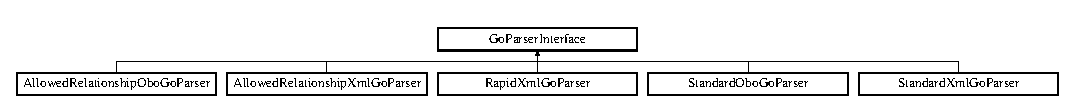
\includegraphics[height=1.061611cm]{classGoParserInterface}
\end{center}
\end{figure}
\subsection*{Public Member Functions}
\begin{DoxyCompactItemize}
\item 
virtual \hyperlink{classGoGraph}{Go\+Graph} $\ast$ \hyperlink{classGoParserInterface_aefde440e0d5404b9efa2a16a89e09674}{parse\+Go\+File} (std\+::string file\+Name)=0
\begin{DoxyCompactList}\small\item\em A pure virtual method for parsing the file and returning a \hyperlink{classGoGraph}{Go\+Graph} object. \end{DoxyCompactList}\item 
virtual bool \hyperlink{classGoParserInterface_a0d2db54063c1ff58a0e15f0187af5aa1}{is\+File\+Good} (const std\+::string \&filename)=0
\begin{DoxyCompactList}\small\item\em A pure virtual method for parsing the file and returning a \hyperlink{classGoGraph}{Go\+Graph} object. \end{DoxyCompactList}\item 
virtual \hyperlink{classGoParserInterface}{Go\+Parser\+Interface} $\ast$ \hyperlink{classGoParserInterface_a21c4ea01809737ab2975fb71edf6fcd5}{clone} ()=0
\begin{DoxyCompactList}\small\item\em A pure virtual clone function for factory pattern. \end{DoxyCompactList}\end{DoxyCompactItemize}


\subsection{Detailed Description}
An interface class to define go graph parsers. 

This class defines the interface of a go graph parser. Pure virtual methods require that parsers implement these methods. 

\subsection{Member Function Documentation}
\index{Go\+Parser\+Interface@{Go\+Parser\+Interface}!clone@{clone}}
\index{clone@{clone}!Go\+Parser\+Interface@{Go\+Parser\+Interface}}
\subsubsection[{\texorpdfstring{clone()=0}{clone()=0}}]{\setlength{\rightskip}{0pt plus 5cm}virtual {\bf Go\+Parser\+Interface}$\ast$ Go\+Parser\+Interface\+::clone (
\begin{DoxyParamCaption}
{}
\end{DoxyParamCaption}
)\hspace{0.3cm}{\ttfamily [pure virtual]}}\hypertarget{classGoParserInterface_a21c4ea01809737ab2975fb71edf6fcd5}{}\label{classGoParserInterface_a21c4ea01809737ab2975fb71edf6fcd5}


A pure virtual clone function for factory pattern. 

This pure virtual method returns an instance of this interface. This method is used in a factory class to have the ability to decide the parser at runtime. 

Implemented in \hyperlink{classAllowedRelationshipOboGoParser_add9a434ad4acd785b51550dc5fd9388b}{Allowed\+Relationship\+Obo\+Go\+Parser}, \hyperlink{classAllowedRelationshipXmlGoParser_a3c330bc9f1ccf6422488bf1ea593f52a}{Allowed\+Relationship\+Xml\+Go\+Parser}, \hyperlink{classRapidXmlGoParser_af69641207e01be186f523939ce03f847}{Rapid\+Xml\+Go\+Parser}, \hyperlink{classStandardXmlGoParser_ac05cc1de0c2fc74e089169f9baea1f0d}{Standard\+Xml\+Go\+Parser}, and \hyperlink{classStandardOboGoParser_aa4c7c326bf20327645fe6df7d57e3fc3}{Standard\+Obo\+Go\+Parser}.

\index{Go\+Parser\+Interface@{Go\+Parser\+Interface}!is\+File\+Good@{is\+File\+Good}}
\index{is\+File\+Good@{is\+File\+Good}!Go\+Parser\+Interface@{Go\+Parser\+Interface}}
\subsubsection[{\texorpdfstring{is\+File\+Good(const std\+::string \&filename)=0}{isFileGood(const std::string &filename)=0}}]{\setlength{\rightskip}{0pt plus 5cm}virtual bool Go\+Parser\+Interface\+::is\+File\+Good (
\begin{DoxyParamCaption}
\item[{const std\+::string \&}]{filename}
\end{DoxyParamCaption}
)\hspace{0.3cm}{\ttfamily [pure virtual]}}\hypertarget{classGoParserInterface_a0d2db54063c1ff58a0e15f0187af5aa1}{}\label{classGoParserInterface_a0d2db54063c1ff58a0e15f0187af5aa1}


A pure virtual method for parsing the file and returning a \hyperlink{classGoGraph}{Go\+Graph} object. 

This pure virtual method requires any parser to have a method that takes a filename string and returns a \hyperlink{classGoGraph}{Go\+Graph} object pointer. 

Implemented in \hyperlink{classAllowedRelationshipOboGoParser_a67722c03da0ca2e0f9eb4008dddc6e06}{Allowed\+Relationship\+Obo\+Go\+Parser}, \hyperlink{classAllowedRelationshipXmlGoParser_a75e964bc34f575bc6c00c56b43f91d0e}{Allowed\+Relationship\+Xml\+Go\+Parser}, \hyperlink{classRapidXmlGoParser_a945a31fd86bd35720d4158caa35302da}{Rapid\+Xml\+Go\+Parser}, \hyperlink{classStandardXmlGoParser_a74c344440ef2ce5b30536e09691c92ab}{Standard\+Xml\+Go\+Parser}, and \hyperlink{classStandardOboGoParser_af6c430101cecf73606ae979d4de6ea7f}{Standard\+Obo\+Go\+Parser}.

\index{Go\+Parser\+Interface@{Go\+Parser\+Interface}!parse\+Go\+File@{parse\+Go\+File}}
\index{parse\+Go\+File@{parse\+Go\+File}!Go\+Parser\+Interface@{Go\+Parser\+Interface}}
\subsubsection[{\texorpdfstring{parse\+Go\+File(std\+::string file\+Name)=0}{parseGoFile(std::string fileName)=0}}]{\setlength{\rightskip}{0pt plus 5cm}virtual {\bf Go\+Graph}$\ast$ Go\+Parser\+Interface\+::parse\+Go\+File (
\begin{DoxyParamCaption}
\item[{std\+::string}]{file\+Name}
\end{DoxyParamCaption}
)\hspace{0.3cm}{\ttfamily [pure virtual]}}\hypertarget{classGoParserInterface_aefde440e0d5404b9efa2a16a89e09674}{}\label{classGoParserInterface_aefde440e0d5404b9efa2a16a89e09674}


A pure virtual method for parsing the file and returning a \hyperlink{classGoGraph}{Go\+Graph} object. 

This pure virtual method requires any parser to have a method that takes a filename string and returns a \hyperlink{classGoGraph}{Go\+Graph} object pointer. 

Implemented in \hyperlink{classAllowedRelationshipOboGoParser_a6eb0ab84216c386a2595aa47233448ad}{Allowed\+Relationship\+Obo\+Go\+Parser}, \hyperlink{classAllowedRelationshipXmlGoParser_ad6e002e7cd0994866b62dba0896d3d24}{Allowed\+Relationship\+Xml\+Go\+Parser}, \hyperlink{classStandardXmlGoParser_ae56413ab11d1fa8f3870f5bcc262d3f8}{Standard\+Xml\+Go\+Parser}, \hyperlink{classRapidXmlGoParser_a7c42085d86c58983601fdada4aaacd9d}{Rapid\+Xml\+Go\+Parser}, and \hyperlink{classStandardOboGoParser_a4eb0d67f0c78456d1e0a9a3f55294424}{Standard\+Obo\+Go\+Parser}.



The documentation for this class was generated from the following file\+:\begin{DoxyCompactItemize}
\item 
ggtk/Go\+Parser\+Interface.\+hpp\end{DoxyCompactItemize}

\hypertarget{classJaccardSetSimilarity}{}\section{Jaccard\+Set\+Similarity Class Reference}
\label{classJaccardSetSimilarity}\index{Jaccard\+Set\+Similarity@{Jaccard\+Set\+Similarity}}


A class to calculate jaccard similarity between 2 sets.  




{\ttfamily \#include $<$ggtk/\+Jaccard\+Set\+Similarity.\+hpp$>$}

Inheritance diagram for Jaccard\+Set\+Similarity\+:\begin{figure}[H]
\begin{center}
\leavevmode
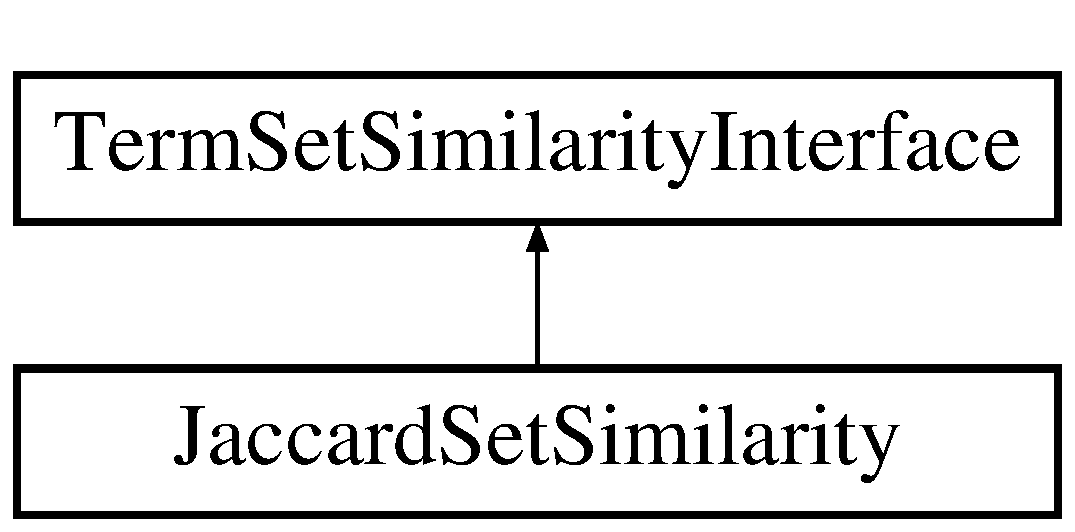
\includegraphics[height=2.000000cm]{classJaccardSetSimilarity}
\end{center}
\end{figure}
\subsection*{Public Member Functions}
\begin{DoxyCompactItemize}
\item 
\hyperlink{classJaccardSetSimilarity_a91ae983223bd59f776c029c1c63f979d}{Jaccard\+Set\+Similarity} ()
\begin{DoxyCompactList}\small\item\em Constructor. \end{DoxyCompactList}\item 
double \hyperlink{classJaccardSetSimilarity_a122a04f7f67b96e393fcde1025a306c3}{calculate\+Similarity} (const boost\+::unordered\+\_\+set$<$ std\+::string $>$ \&termsA, const boost\+::unordered\+\_\+set$<$ std\+::string $>$ \&termsB)
\begin{DoxyCompactList}\small\item\em A method for calculating term set to term set similarity for \hyperlink{namespaceGO}{GO} terms;. \end{DoxyCompactList}\end{DoxyCompactItemize}


\subsection{Detailed Description}
A class to calculate jaccard similarity between 2 sets. 

This class calculates jaccard set similarity between two sets of terms. 

\subsection{Constructor \& Destructor Documentation}
\index{Jaccard\+Set\+Similarity@{Jaccard\+Set\+Similarity}!Jaccard\+Set\+Similarity@{Jaccard\+Set\+Similarity}}
\index{Jaccard\+Set\+Similarity@{Jaccard\+Set\+Similarity}!Jaccard\+Set\+Similarity@{Jaccard\+Set\+Similarity}}
\subsubsection[{\texorpdfstring{Jaccard\+Set\+Similarity()}{JaccardSetSimilarity()}}]{\setlength{\rightskip}{0pt plus 5cm}Jaccard\+Set\+Similarity\+::\+Jaccard\+Set\+Similarity (
\begin{DoxyParamCaption}
{}
\end{DoxyParamCaption}
)\hspace{0.3cm}{\ttfamily [inline]}}\hypertarget{classJaccardSetSimilarity_a91ae983223bd59f776c029c1c63f979d}{}\label{classJaccardSetSimilarity_a91ae983223bd59f776c029c1c63f979d}


Constructor. 

Creates the \hyperlink{classJaccardSetSimilarity}{Jaccard\+Set\+Similarity} class. 

\subsection{Member Function Documentation}
\index{Jaccard\+Set\+Similarity@{Jaccard\+Set\+Similarity}!calculate\+Similarity@{calculate\+Similarity}}
\index{calculate\+Similarity@{calculate\+Similarity}!Jaccard\+Set\+Similarity@{Jaccard\+Set\+Similarity}}
\subsubsection[{\texorpdfstring{calculate\+Similarity(const boost\+::unordered\+\_\+set$<$ std\+::string $>$ \&terms\+A, const boost\+::unordered\+\_\+set$<$ std\+::string $>$ \&terms\+B)}{calculateSimilarity(const boost::unordered_set< std::string > &termsA, const boost::unordered_set< std::string > &termsB)}}]{\setlength{\rightskip}{0pt plus 5cm}double Jaccard\+Set\+Similarity\+::calculate\+Similarity (
\begin{DoxyParamCaption}
\item[{const boost\+::unordered\+\_\+set$<$ std\+::string $>$ \&}]{termsA, }
\item[{const boost\+::unordered\+\_\+set$<$ std\+::string $>$ \&}]{termsB}
\end{DoxyParamCaption}
)\hspace{0.3cm}{\ttfamily [inline]}, {\ttfamily [virtual]}}\hypertarget{classJaccardSetSimilarity_a122a04f7f67b96e393fcde1025a306c3}{}\label{classJaccardSetSimilarity_a122a04f7f67b96e393fcde1025a306c3}


A method for calculating term set to term set similarity for \hyperlink{namespaceGO}{GO} terms;. 

This method returns the Jaccard set similarity. 

Implements \hyperlink{classTermSetSimilarityInterface_aeb985b714efc3df40e55bdd31e425e04}{Term\+Set\+Similarity\+Interface}.



The documentation for this class was generated from the following file\+:\begin{DoxyCompactItemize}
\item 
ggtk/Jaccard\+Set\+Similarity.\+hpp\end{DoxyCompactItemize}

\hypertarget{classJiangConrathSimilarity}{}\section{Jiang\+Conrath\+Similarity Class Reference}
\label{classJiangConrathSimilarity}\index{Jiang\+Conrath\+Similarity@{Jiang\+Conrath\+Similarity}}


A class to calculate Jiang Conrath similarity between 2 terms.  




{\ttfamily \#include $<$ggtk/\+Jiang\+Conrath\+Similarity.\+hpp$>$}

Inheritance diagram for Jiang\+Conrath\+Similarity\+:\begin{figure}[H]
\begin{center}
\leavevmode
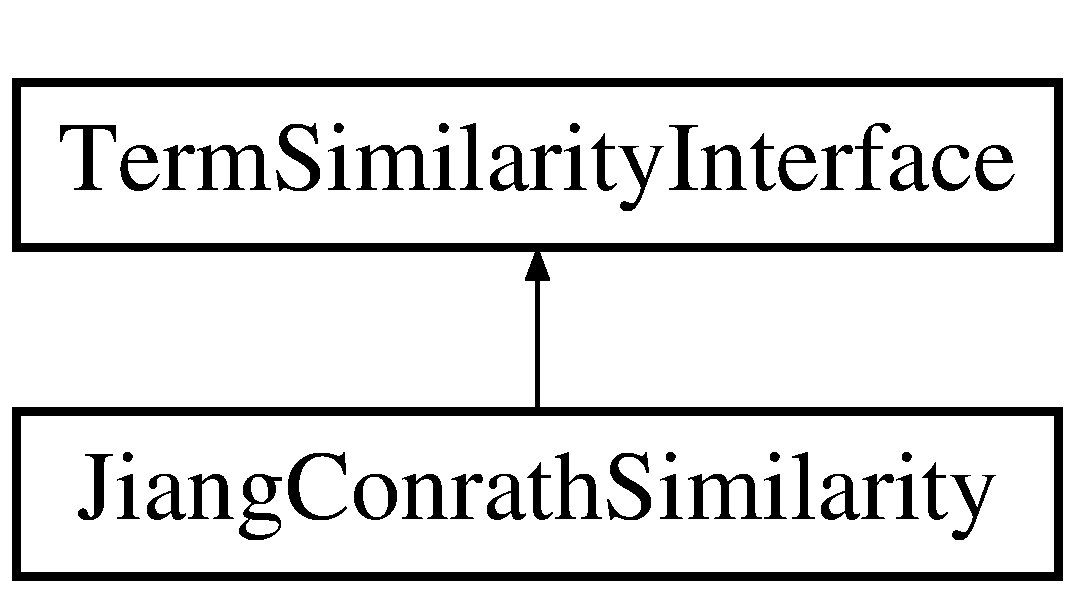
\includegraphics[height=2.000000cm]{classJiangConrathSimilarity}
\end{center}
\end{figure}
\subsection*{Public Member Functions}
\begin{DoxyCompactItemize}
\item 
\hyperlink{classJiangConrathSimilarity_addd16c8b26721f64b954c3006aa2ed26}{Jiang\+Conrath\+Similarity} (\hyperlink{classGoGraph}{Go\+Graph} $\ast$go\+Graph, \hyperlink{classTermInformationContentMap}{Term\+Information\+Content\+Map} \&ic\+Map)
\begin{DoxyCompactList}\small\item\em A constructor. \end{DoxyCompactList}\item 
double \hyperlink{classJiangConrathSimilarity_a110fcc0d8b68b6dde9e90d897c859034}{calculate\+Term\+Similarity} (std\+::string go\+TermA, std\+::string go\+TermB)
\begin{DoxyCompactList}\small\item\em A method for calculating term-\/to-\/term similarity for \hyperlink{namespaceGO}{GO} terms using Jiang\+Conrath similarity. \end{DoxyCompactList}\item 
double \hyperlink{classJiangConrathSimilarity_a489dcbef15f4a5063af79cb03920cdf9}{calculate\+Normalized\+Term\+Similarity} (std\+::string go\+TermA, std\+::string go\+TermB)
\begin{DoxyCompactList}\small\item\em A method for calculating term-\/to-\/term similarity for \hyperlink{namespaceGO}{GO} terms using Normalized Jiang\+Conrath similarity. \end{DoxyCompactList}\item 
std\+::string \hyperlink{classJiangConrathSimilarity_a9a72b8c9687bfd578d8c51ec8564e87c}{get\+M\+I\+CA} (boost\+::unordered\+\_\+set$<$ std\+::string $>$ \&ancestorsA, boost\+::unordered\+\_\+set$<$ std\+::string $>$ \&ancestorsB)
\begin{DoxyCompactList}\small\item\em A method for calculating the most informative common ancestor. \end{DoxyCompactList}\end{DoxyCompactItemize}


\subsection{Detailed Description}
A class to calculate Jiang Conrath similarity between 2 terms. 

This class calculates Jiang Conrath similarity.

Jiang, J. J., \& Conrath, D. W. (1997). Semantic similarity based on corpus statistics and lexical taxonomy. In Proc. of 10th International Conference on Research on Computational Linguistics, Taiwan.

P. W. Lord, R. D. Stevens, A. Brass, and C. A. Goble, \char`\"{}\+Semantic similarity measures as tools for exploring the gene ontology,\char`\"{} Pac Symp Biocomput, pp. 601-\/12, 2003.

distance = I\+C(term\+A) + I\+C(term\+B) -\/ 2$\ast$\+IC(M\+I\+CA) max\+Distance = 2$\ast$\+IC(single annotaiotn) similarity = 1 -\/ distance/max\+Distance (see Lord et al.) 

\subsection{Constructor \& Destructor Documentation}
\index{Jiang\+Conrath\+Similarity@{Jiang\+Conrath\+Similarity}!Jiang\+Conrath\+Similarity@{Jiang\+Conrath\+Similarity}}
\index{Jiang\+Conrath\+Similarity@{Jiang\+Conrath\+Similarity}!Jiang\+Conrath\+Similarity@{Jiang\+Conrath\+Similarity}}
\subsubsection[{\texorpdfstring{Jiang\+Conrath\+Similarity(\+Go\+Graph $\ast$go\+Graph, Term\+Information\+Content\+Map \&ic\+Map)}{JiangConrathSimilarity(GoGraph *goGraph, TermInformationContentMap &icMap)}}]{\setlength{\rightskip}{0pt plus 5cm}Jiang\+Conrath\+Similarity\+::\+Jiang\+Conrath\+Similarity (
\begin{DoxyParamCaption}
\item[{{\bf Go\+Graph} $\ast$}]{go\+Graph, }
\item[{{\bf Term\+Information\+Content\+Map} \&}]{ic\+Map}
\end{DoxyParamCaption}
)\hspace{0.3cm}{\ttfamily [inline]}}\hypertarget{classJiangConrathSimilarity_addd16c8b26721f64b954c3006aa2ed26}{}\label{classJiangConrathSimilarity_addd16c8b26721f64b954c3006aa2ed26}


A constructor. 

Creates the default(empty) \hyperlink{classStandardRelationshipPolicy}{Standard\+Relationship\+Policy} 

\subsection{Member Function Documentation}
\index{Jiang\+Conrath\+Similarity@{Jiang\+Conrath\+Similarity}!calculate\+Normalized\+Term\+Similarity@{calculate\+Normalized\+Term\+Similarity}}
\index{calculate\+Normalized\+Term\+Similarity@{calculate\+Normalized\+Term\+Similarity}!Jiang\+Conrath\+Similarity@{Jiang\+Conrath\+Similarity}}
\subsubsection[{\texorpdfstring{calculate\+Normalized\+Term\+Similarity(std\+::string go\+Term\+A, std\+::string go\+Term\+B)}{calculateNormalizedTermSimilarity(std::string goTermA, std::string goTermB)}}]{\setlength{\rightskip}{0pt plus 5cm}double Jiang\+Conrath\+Similarity\+::calculate\+Normalized\+Term\+Similarity (
\begin{DoxyParamCaption}
\item[{std\+::string}]{go\+TermA, }
\item[{std\+::string}]{go\+TermB}
\end{DoxyParamCaption}
)\hspace{0.3cm}{\ttfamily [inline]}, {\ttfamily [virtual]}}\hypertarget{classJiangConrathSimilarity_a489dcbef15f4a5063af79cb03920cdf9}{}\label{classJiangConrathSimilarity_a489dcbef15f4a5063af79cb03920cdf9}


A method for calculating term-\/to-\/term similarity for \hyperlink{namespaceGO}{GO} terms using Normalized Jiang\+Conrath similarity. 

This method returns the Jiang\+Conrath similarity scaled between 0 and 1 \mbox{[}0,1\mbox{]} inclusive 

Implements \hyperlink{classTermSimilarityInterface_aa46b7870c7725faab85ec502a3e5242d}{Term\+Similarity\+Interface}.

\index{Jiang\+Conrath\+Similarity@{Jiang\+Conrath\+Similarity}!calculate\+Term\+Similarity@{calculate\+Term\+Similarity}}
\index{calculate\+Term\+Similarity@{calculate\+Term\+Similarity}!Jiang\+Conrath\+Similarity@{Jiang\+Conrath\+Similarity}}
\subsubsection[{\texorpdfstring{calculate\+Term\+Similarity(std\+::string go\+Term\+A, std\+::string go\+Term\+B)}{calculateTermSimilarity(std::string goTermA, std::string goTermB)}}]{\setlength{\rightskip}{0pt plus 5cm}double Jiang\+Conrath\+Similarity\+::calculate\+Term\+Similarity (
\begin{DoxyParamCaption}
\item[{std\+::string}]{go\+TermA, }
\item[{std\+::string}]{go\+TermB}
\end{DoxyParamCaption}
)\hspace{0.3cm}{\ttfamily [inline]}, {\ttfamily [virtual]}}\hypertarget{classJiangConrathSimilarity_a110fcc0d8b68b6dde9e90d897c859034}{}\label{classJiangConrathSimilarity_a110fcc0d8b68b6dde9e90d897c859034}


A method for calculating term-\/to-\/term similarity for \hyperlink{namespaceGO}{GO} terms using Jiang\+Conrath similarity. 

This method returns the Jiang\+Conrath similarity or the information content of the most informative common ancestor. 

Implements \hyperlink{classTermSimilarityInterface_ae3474adcfcb02faef65ed5e16ef4db47}{Term\+Similarity\+Interface}.

\index{Jiang\+Conrath\+Similarity@{Jiang\+Conrath\+Similarity}!get\+M\+I\+CA@{get\+M\+I\+CA}}
\index{get\+M\+I\+CA@{get\+M\+I\+CA}!Jiang\+Conrath\+Similarity@{Jiang\+Conrath\+Similarity}}
\subsubsection[{\texorpdfstring{get\+M\+I\+C\+A(boost\+::unordered\+\_\+set$<$ std\+::string $>$ \&ancestors\+A, boost\+::unordered\+\_\+set$<$ std\+::string $>$ \&ancestors\+B)}{getMICA(boost::unordered_set< std::string > &ancestorsA, boost::unordered_set< std::string > &ancestorsB)}}]{\setlength{\rightskip}{0pt plus 5cm}std\+::string Jiang\+Conrath\+Similarity\+::get\+M\+I\+CA (
\begin{DoxyParamCaption}
\item[{boost\+::unordered\+\_\+set$<$ std\+::string $>$ \&}]{ancestorsA, }
\item[{boost\+::unordered\+\_\+set$<$ std\+::string $>$ \&}]{ancestorsB}
\end{DoxyParamCaption}
)\hspace{0.3cm}{\ttfamily [inline]}}\hypertarget{classJiangConrathSimilarity_a9a72b8c9687bfd578d8c51ec8564e87c}{}\label{classJiangConrathSimilarity_a9a72b8c9687bfd578d8c51ec8564e87c}


A method for calculating the most informative common ancestor. 

This method searches the sets to determine the most informatics ancestor. 

The documentation for this class was generated from the following file\+:\begin{DoxyCompactItemize}
\item 
ggtk/Jiang\+Conrath\+Similarity.\+hpp\end{DoxyCompactItemize}

\hypertarget{classLinSimilarity}{}\section{Lin\+Similarity Class Reference}
\label{classLinSimilarity}\index{Lin\+Similarity@{Lin\+Similarity}}


A class to calculate Lin similarity between 2 terms.  




{\ttfamily \#include $<$ggtk/\+Lin\+Similarity.\+hpp$>$}

Inheritance diagram for Lin\+Similarity\+:\begin{figure}[H]
\begin{center}
\leavevmode
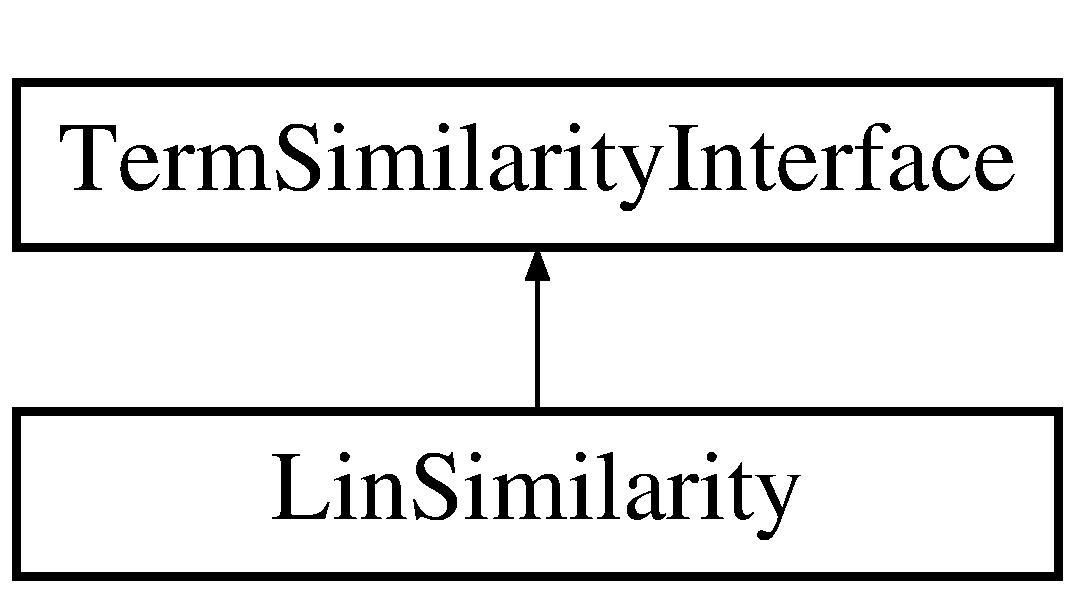
\includegraphics[height=2.000000cm]{classLinSimilarity}
\end{center}
\end{figure}
\subsection*{Public Member Functions}
\begin{DoxyCompactItemize}
\item 
\hyperlink{classLinSimilarity_a44739dba8ae706d5248615bd9df9cc31}{Lin\+Similarity} (\hyperlink{classGoGraph}{Go\+Graph} $\ast$go\+Graph, \hyperlink{classTermInformationContentMap}{Term\+Information\+Content\+Map} \&ic\+Map)
\begin{DoxyCompactList}\small\item\em A constructor. \end{DoxyCompactList}\item 
double \hyperlink{classLinSimilarity_a55d2d8bd6aea6fc3e9b0920f05828a15}{calculate\+Term\+Similarity} (std\+::string go\+TermA, std\+::string go\+TermB)
\begin{DoxyCompactList}\small\item\em A method for calculating term-\/to-\/term similarity for \hyperlink{namespaceGO}{GO} terms using Lin similarity. \end{DoxyCompactList}\item 
double \hyperlink{classLinSimilarity_a576df5bf234556e57e2ddcfda3d73b93}{calculate\+Normalized\+Term\+Similarity} (std\+::string go\+TermA, std\+::string go\+TermB)
\begin{DoxyCompactList}\small\item\em A method for calculating term-\/to-\/term similarity for \hyperlink{namespaceGO}{GO} terms using Normalized Lin similarity. \end{DoxyCompactList}\item 
std\+::string \hyperlink{classLinSimilarity_ab2e39eac3cf61be4e1b44b988fa6f490}{get\+M\+I\+CA} (boost\+::unordered\+\_\+set$<$ std\+::string $>$ \&ancestorsA, boost\+::unordered\+\_\+set$<$ std\+::string $>$ \&ancestorsB)
\begin{DoxyCompactList}\small\item\em A method for calculating the most informative common ancestor. \end{DoxyCompactList}\end{DoxyCompactItemize}


\subsection{Detailed Description}
A class to calculate Lin similarity between 2 terms. 

This class calculates Lin similarity.

Lin, D. (1998) An information theoretic definition of similarity. In\+: Proc. of the 15th Inernational Conference on Machine Learning. San Franscisco, CA\+: Morgan Kaufman. pp 296-\/304

P. W. Lord, R. D. Stevens, A. Brass, and C. A. Goble, \char`\"{}\+Semantic similarity measures as tools for exploring the gene ontology,\char`\"{} Pac Symp Biocomput, pp. 601-\/12, 2003.

2 $\ast$ I\+C(\+M\+I\+C\+A) / ( I\+C(term\+A) + I\+C(term\+B) ) 

\subsection{Constructor \& Destructor Documentation}
\index{Lin\+Similarity@{Lin\+Similarity}!Lin\+Similarity@{Lin\+Similarity}}
\index{Lin\+Similarity@{Lin\+Similarity}!Lin\+Similarity@{Lin\+Similarity}}
\subsubsection[{\texorpdfstring{Lin\+Similarity(\+Go\+Graph $\ast$go\+Graph, Term\+Information\+Content\+Map \&ic\+Map)}{LinSimilarity(GoGraph *goGraph, TermInformationContentMap &icMap)}}]{\setlength{\rightskip}{0pt plus 5cm}Lin\+Similarity\+::\+Lin\+Similarity (
\begin{DoxyParamCaption}
\item[{{\bf Go\+Graph} $\ast$}]{go\+Graph, }
\item[{{\bf Term\+Information\+Content\+Map} \&}]{ic\+Map}
\end{DoxyParamCaption}
)\hspace{0.3cm}{\ttfamily [inline]}}\hypertarget{classLinSimilarity_a44739dba8ae706d5248615bd9df9cc31}{}\label{classLinSimilarity_a44739dba8ae706d5248615bd9df9cc31}


A constructor. 

Creates the \hyperlink{classLinSimilarity}{Lin\+Similarity} calculator 

\subsection{Member Function Documentation}
\index{Lin\+Similarity@{Lin\+Similarity}!calculate\+Normalized\+Term\+Similarity@{calculate\+Normalized\+Term\+Similarity}}
\index{calculate\+Normalized\+Term\+Similarity@{calculate\+Normalized\+Term\+Similarity}!Lin\+Similarity@{Lin\+Similarity}}
\subsubsection[{\texorpdfstring{calculate\+Normalized\+Term\+Similarity(std\+::string go\+Term\+A, std\+::string go\+Term\+B)}{calculateNormalizedTermSimilarity(std::string goTermA, std::string goTermB)}}]{\setlength{\rightskip}{0pt plus 5cm}double Lin\+Similarity\+::calculate\+Normalized\+Term\+Similarity (
\begin{DoxyParamCaption}
\item[{std\+::string}]{go\+TermA, }
\item[{std\+::string}]{go\+TermB}
\end{DoxyParamCaption}
)\hspace{0.3cm}{\ttfamily [inline]}, {\ttfamily [virtual]}}\hypertarget{classLinSimilarity_a576df5bf234556e57e2ddcfda3d73b93}{}\label{classLinSimilarity_a576df5bf234556e57e2ddcfda3d73b93}


A method for calculating term-\/to-\/term similarity for \hyperlink{namespaceGO}{GO} terms using Normalized Lin similarity. 

This method returns the Lin similarity scaled between 0 and 1 \mbox{[}0,1\mbox{]} inclusive 

Implements \hyperlink{classTermSimilarityInterface_aa46b7870c7725faab85ec502a3e5242d}{Term\+Similarity\+Interface}.

\index{Lin\+Similarity@{Lin\+Similarity}!calculate\+Term\+Similarity@{calculate\+Term\+Similarity}}
\index{calculate\+Term\+Similarity@{calculate\+Term\+Similarity}!Lin\+Similarity@{Lin\+Similarity}}
\subsubsection[{\texorpdfstring{calculate\+Term\+Similarity(std\+::string go\+Term\+A, std\+::string go\+Term\+B)}{calculateTermSimilarity(std::string goTermA, std::string goTermB)}}]{\setlength{\rightskip}{0pt plus 5cm}double Lin\+Similarity\+::calculate\+Term\+Similarity (
\begin{DoxyParamCaption}
\item[{std\+::string}]{go\+TermA, }
\item[{std\+::string}]{go\+TermB}
\end{DoxyParamCaption}
)\hspace{0.3cm}{\ttfamily [inline]}, {\ttfamily [virtual]}}\hypertarget{classLinSimilarity_a55d2d8bd6aea6fc3e9b0920f05828a15}{}\label{classLinSimilarity_a55d2d8bd6aea6fc3e9b0920f05828a15}


A method for calculating term-\/to-\/term similarity for \hyperlink{namespaceGO}{GO} terms using Lin similarity. 

This method returns the Lin similarity. 

Implements \hyperlink{classTermSimilarityInterface_ae3474adcfcb02faef65ed5e16ef4db47}{Term\+Similarity\+Interface}.

\index{Lin\+Similarity@{Lin\+Similarity}!get\+M\+I\+CA@{get\+M\+I\+CA}}
\index{get\+M\+I\+CA@{get\+M\+I\+CA}!Lin\+Similarity@{Lin\+Similarity}}
\subsubsection[{\texorpdfstring{get\+M\+I\+C\+A(boost\+::unordered\+\_\+set$<$ std\+::string $>$ \&ancestors\+A, boost\+::unordered\+\_\+set$<$ std\+::string $>$ \&ancestors\+B)}{getMICA(boost::unordered_set< std::string > &ancestorsA, boost::unordered_set< std::string > &ancestorsB)}}]{\setlength{\rightskip}{0pt plus 5cm}std\+::string Lin\+Similarity\+::get\+M\+I\+CA (
\begin{DoxyParamCaption}
\item[{boost\+::unordered\+\_\+set$<$ std\+::string $>$ \&}]{ancestorsA, }
\item[{boost\+::unordered\+\_\+set$<$ std\+::string $>$ \&}]{ancestorsB}
\end{DoxyParamCaption}
)\hspace{0.3cm}{\ttfamily [inline]}}\hypertarget{classLinSimilarity_ab2e39eac3cf61be4e1b44b988fa6f490}{}\label{classLinSimilarity_ab2e39eac3cf61be4e1b44b988fa6f490}


A method for calculating the most informative common ancestor. 

This method searches the sets to determine the most informatics ancestor. 

The documentation for this class was generated from the following file\+:\begin{DoxyCompactItemize}
\item 
ggtk/Lin\+Similarity.\+hpp\end{DoxyCompactItemize}

\hypertarget{classMgiAnnotationParser}{}\section{Mgi\+Annotation\+Parser Class Reference}
\label{classMgiAnnotationParser}\index{Mgi\+Annotation\+Parser@{Mgi\+Annotation\+Parser}}


A class to parse an Mouse Genome Informatics go annotation file.  




{\ttfamily \#include $<$ggtk/\+Mgi\+Annotation\+Parser.\+hpp$>$}

Inheritance diagram for Mgi\+Annotation\+Parser\+:\begin{figure}[H]
\begin{center}
\leavevmode
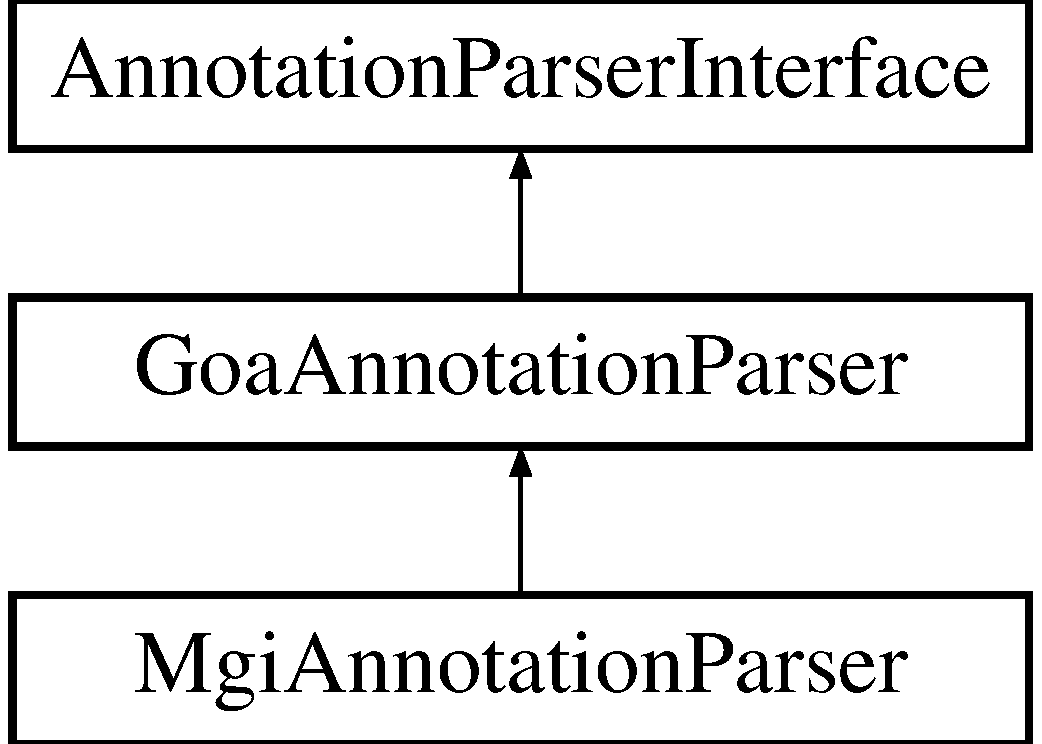
\includegraphics[height=3.000000cm]{classMgiAnnotationParser}
\end{center}
\end{figure}
\subsection*{Public Member Functions}
\begin{DoxyCompactItemize}
\item 
\hyperlink{classMgiAnnotationParser_a2f7a0d1080bf0a338ac35f9cd558da20}{Mgi\+Annotation\+Parser} ()
\begin{DoxyCompactList}\small\item\em A default constructor method for creating the parser. \end{DoxyCompactList}\item 
\hyperlink{classMgiAnnotationParser_ad21111f35a5476970585eb84d7ffbf70}{Mgi\+Annotation\+Parser} (\hyperlink{classEvidencePolicyInterface}{Evidence\+Policy\+Interface} $\ast$policy)
\begin{DoxyCompactList}\small\item\em A parameterized constructor method for creating the parser with a policy. \end{DoxyCompactList}\end{DoxyCompactItemize}


\subsection{Detailed Description}
A class to parse an Mouse Genome Informatics go annotation file. 

This class will read an mgi annotation file and add those annoations to an \hyperlink{classAnnotationData}{Annotation\+Data} class. Available at\+: \href{ftp://ftp.informatics.jax.org/pub/reports/index.html#go}{\tt ftp\+://ftp.\+informatics.\+jax.\+org/pub/reports/index.\+html\#go}

M\+GI uses G\+AF format which is G\+OA.

Implements \hyperlink{classAnnotationParserInterface}{Annotation\+Parser\+Interface} 

\subsection{Constructor \& Destructor Documentation}
\index{Mgi\+Annotation\+Parser@{Mgi\+Annotation\+Parser}!Mgi\+Annotation\+Parser@{Mgi\+Annotation\+Parser}}
\index{Mgi\+Annotation\+Parser@{Mgi\+Annotation\+Parser}!Mgi\+Annotation\+Parser@{Mgi\+Annotation\+Parser}}
\subsubsection[{\texorpdfstring{Mgi\+Annotation\+Parser()}{MgiAnnotationParser()}}]{\setlength{\rightskip}{0pt plus 5cm}Mgi\+Annotation\+Parser\+::\+Mgi\+Annotation\+Parser (
\begin{DoxyParamCaption}
{}
\end{DoxyParamCaption}
)\hspace{0.3cm}{\ttfamily [inline]}}\hypertarget{classMgiAnnotationParser_a2f7a0d1080bf0a338ac35f9cd558da20}{}\label{classMgiAnnotationParser_a2f7a0d1080bf0a338ac35f9cd558da20}


A default constructor method for creating the parser. 

Creates the parser \index{Mgi\+Annotation\+Parser@{Mgi\+Annotation\+Parser}!Mgi\+Annotation\+Parser@{Mgi\+Annotation\+Parser}}
\index{Mgi\+Annotation\+Parser@{Mgi\+Annotation\+Parser}!Mgi\+Annotation\+Parser@{Mgi\+Annotation\+Parser}}
\subsubsection[{\texorpdfstring{Mgi\+Annotation\+Parser(\+Evidence\+Policy\+Interface $\ast$policy)}{MgiAnnotationParser(EvidencePolicyInterface *policy)}}]{\setlength{\rightskip}{0pt plus 5cm}Mgi\+Annotation\+Parser\+::\+Mgi\+Annotation\+Parser (
\begin{DoxyParamCaption}
\item[{{\bf Evidence\+Policy\+Interface} $\ast$}]{policy}
\end{DoxyParamCaption}
)\hspace{0.3cm}{\ttfamily [inline]}}\hypertarget{classMgiAnnotationParser_ad21111f35a5476970585eb84d7ffbf70}{}\label{classMgiAnnotationParser_ad21111f35a5476970585eb84d7ffbf70}


A parameterized constructor method for creating the parser with a policy. 

Creates the parser with a custom policy 

The documentation for this class was generated from the following file\+:\begin{DoxyCompactItemize}
\item 
ggtk/Mgi\+Annotation\+Parser.\+hpp\end{DoxyCompactItemize}

\hypertarget{classMICASharedInformation}{}\section{M\+I\+C\+A\+Shared\+Information Class Reference}
\label{classMICASharedInformation}\index{M\+I\+C\+A\+Shared\+Information@{M\+I\+C\+A\+Shared\+Information}}


A class to calculate shared infromation as the most informative common ancestor (M\+I\+CA)  




{\ttfamily \#include $<$ggtk/\+M\+I\+C\+A\+Shared\+Information.\+hpp$>$}

Inheritance diagram for M\+I\+C\+A\+Shared\+Information\+:\begin{figure}[H]
\begin{center}
\leavevmode
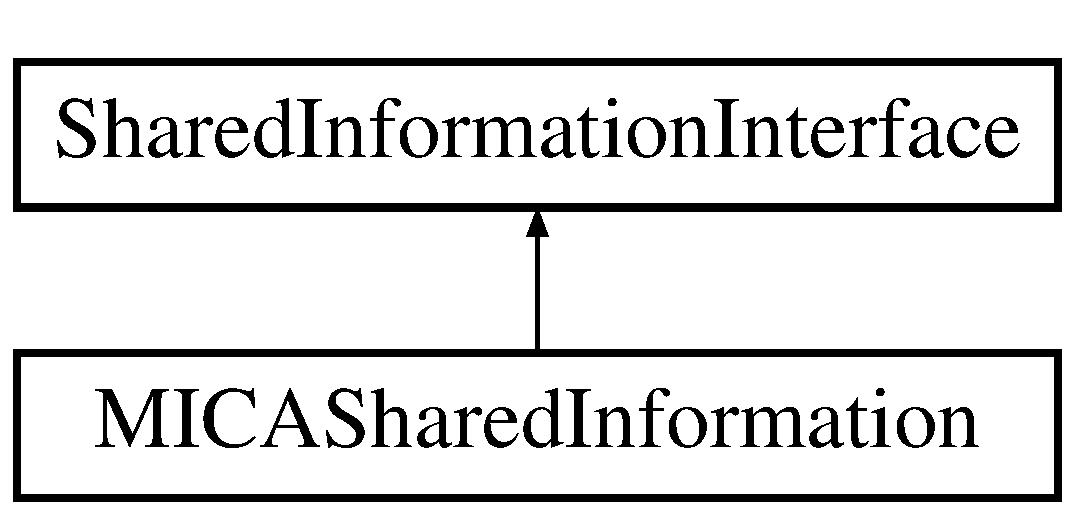
\includegraphics[height=2.000000cm]{classMICASharedInformation}
\end{center}
\end{figure}
\subsection*{Public Member Functions}
\begin{DoxyCompactItemize}
\item 
\hyperlink{classMICASharedInformation_a6f377d93f091f1b03511d4e107a0b54b}{M\+I\+C\+A\+Shared\+Information} (\hyperlink{classGoGraph}{Go\+Graph} $\ast$go\+Graph, \hyperlink{classTermInformationContentMap}{Term\+Information\+Content\+Map} \&ic\+Map)
\begin{DoxyCompactList}\small\item\em A constructor. \end{DoxyCompactList}\item 
double \hyperlink{classMICASharedInformation_a8f6329c173f2cd17caf1a65043e8e249}{shared\+Information} (const std\+::string \&termA, const std\+::string \&termB)
\begin{DoxyCompactList}\small\item\em A method for calculating the shared infromation between two concepts. \end{DoxyCompactList}\item 
double \hyperlink{classMICASharedInformation_a230adc046f7f4bbab190aaef25d15a37}{shared\+Information} (const std\+::string \&term)
\begin{DoxyCompactList}\small\item\em An interface method for returning the shared information of a single terms,or information content. \end{DoxyCompactList}\item 
double \hyperlink{classMICASharedInformation_ae88d4a76721e03bbb418eb870fa18ff1}{max\+Information\+Content} (const std\+::string \&term)
\begin{DoxyCompactList}\small\item\em An interface method for returning the maximum information content for a term. \end{DoxyCompactList}\item 
bool \hyperlink{classMICASharedInformation_a0fece18244af62c7e2258b0af418413a}{has\+Term} (const std\+::string \&term)
\begin{DoxyCompactList}\small\item\em An interface method for determining if a term can be found. \end{DoxyCompactList}\item 
bool \hyperlink{classMICASharedInformation_a9cea24c8af57f17248ffe1f12fea9545}{is\+Same\+Ontology} (const std\+::string \&termA, const std\+::string \&termB)
\begin{DoxyCompactList}\small\item\em An interface method for determining if the two terms are of like ontologies. \end{DoxyCompactList}\end{DoxyCompactItemize}


\subsection{Detailed Description}
A class to calculate shared infromation as the most informative common ancestor (M\+I\+CA) 

This class calculates shared infromation using the most informative common ancestor (M\+I\+CA). The M\+I\+CA is a term that is also known as the minimum subsumer.

This shared information method forms the basis of 3 inforamtion content measures put forward by Lord el al.

P. W. Lord, R. D. Stevens, A. Brass, and C. A. Goble, \char`\"{}\+Semantic similarity measures as tools for exploring the gene ontology,\char`\"{} Pac Symp Biocomput, pp. 601-\/12, 2003. 

\subsection{Constructor \& Destructor Documentation}
\index{M\+I\+C\+A\+Shared\+Information@{M\+I\+C\+A\+Shared\+Information}!M\+I\+C\+A\+Shared\+Information@{M\+I\+C\+A\+Shared\+Information}}
\index{M\+I\+C\+A\+Shared\+Information@{M\+I\+C\+A\+Shared\+Information}!M\+I\+C\+A\+Shared\+Information@{M\+I\+C\+A\+Shared\+Information}}
\subsubsection[{\texorpdfstring{M\+I\+C\+A\+Shared\+Information(\+Go\+Graph $\ast$go\+Graph, Term\+Information\+Content\+Map \&ic\+Map)}{MICASharedInformation(GoGraph *goGraph, TermInformationContentMap &icMap)}}]{\setlength{\rightskip}{0pt plus 5cm}M\+I\+C\+A\+Shared\+Information\+::\+M\+I\+C\+A\+Shared\+Information (
\begin{DoxyParamCaption}
\item[{{\bf Go\+Graph} $\ast$}]{go\+Graph, }
\item[{{\bf Term\+Information\+Content\+Map} \&}]{ic\+Map}
\end{DoxyParamCaption}
)\hspace{0.3cm}{\ttfamily [inline]}}\hypertarget{classMICASharedInformation_a6f377d93f091f1b03511d4e107a0b54b}{}\label{classMICASharedInformation_a6f377d93f091f1b03511d4e107a0b54b}


A constructor. 

Creates the \hyperlink{classMICASharedInformation}{M\+I\+C\+A\+Shared\+Information} class 

\subsection{Member Function Documentation}
\index{M\+I\+C\+A\+Shared\+Information@{M\+I\+C\+A\+Shared\+Information}!has\+Term@{has\+Term}}
\index{has\+Term@{has\+Term}!M\+I\+C\+A\+Shared\+Information@{M\+I\+C\+A\+Shared\+Information}}
\subsubsection[{\texorpdfstring{has\+Term(const std\+::string \&term)}{hasTerm(const std::string &term)}}]{\setlength{\rightskip}{0pt plus 5cm}bool M\+I\+C\+A\+Shared\+Information\+::has\+Term (
\begin{DoxyParamCaption}
\item[{const std\+::string \&}]{term}
\end{DoxyParamCaption}
)\hspace{0.3cm}{\ttfamily [inline]}, {\ttfamily [virtual]}}\hypertarget{classMICASharedInformation_a0fece18244af62c7e2258b0af418413a}{}\label{classMICASharedInformation_a0fece18244af62c7e2258b0af418413a}


An interface method for determining if a term can be found. 

Determines if the term can be found in the current map. 

Implements \hyperlink{classSharedInformationInterface_a3f056cf6a40eea8c1669108087dcd5c8}{Shared\+Information\+Interface}.

\index{M\+I\+C\+A\+Shared\+Information@{M\+I\+C\+A\+Shared\+Information}!is\+Same\+Ontology@{is\+Same\+Ontology}}
\index{is\+Same\+Ontology@{is\+Same\+Ontology}!M\+I\+C\+A\+Shared\+Information@{M\+I\+C\+A\+Shared\+Information}}
\subsubsection[{\texorpdfstring{is\+Same\+Ontology(const std\+::string \&term\+A, const std\+::string \&term\+B)}{isSameOntology(const std::string &termA, const std::string &termB)}}]{\setlength{\rightskip}{0pt plus 5cm}bool M\+I\+C\+A\+Shared\+Information\+::is\+Same\+Ontology (
\begin{DoxyParamCaption}
\item[{const std\+::string \&}]{termA, }
\item[{const std\+::string \&}]{termB}
\end{DoxyParamCaption}
)\hspace{0.3cm}{\ttfamily [inline]}, {\ttfamily [virtual]}}\hypertarget{classMICASharedInformation_a9cea24c8af57f17248ffe1f12fea9545}{}\label{classMICASharedInformation_a9cea24c8af57f17248ffe1f12fea9545}


An interface method for determining if the two terms are of like ontologies. 

Determine if two terms are of the same ontology. 

Implements \hyperlink{classSharedInformationInterface_a607463b9736df9c4b8ec3ba9fe41c19d}{Shared\+Information\+Interface}.

\index{M\+I\+C\+A\+Shared\+Information@{M\+I\+C\+A\+Shared\+Information}!max\+Information\+Content@{max\+Information\+Content}}
\index{max\+Information\+Content@{max\+Information\+Content}!M\+I\+C\+A\+Shared\+Information@{M\+I\+C\+A\+Shared\+Information}}
\subsubsection[{\texorpdfstring{max\+Information\+Content(const std\+::string \&term)}{maxInformationContent(const std::string &term)}}]{\setlength{\rightskip}{0pt plus 5cm}double M\+I\+C\+A\+Shared\+Information\+::max\+Information\+Content (
\begin{DoxyParamCaption}
\item[{const std\+::string \&}]{term}
\end{DoxyParamCaption}
)\hspace{0.3cm}{\ttfamily [inline]}, {\ttfamily [virtual]}}\hypertarget{classMICASharedInformation_ae88d4a76721e03bbb418eb870fa18ff1}{}\label{classMICASharedInformation_ae88d4a76721e03bbb418eb870fa18ff1}


An interface method for returning the maximum information content for a term. 

This method provides the absolute max information content within a corpus for normalization purposes. 

Implements \hyperlink{classSharedInformationInterface_a7356ba99509458777972ce0f00ebd999}{Shared\+Information\+Interface}.

\index{M\+I\+C\+A\+Shared\+Information@{M\+I\+C\+A\+Shared\+Information}!shared\+Information@{shared\+Information}}
\index{shared\+Information@{shared\+Information}!M\+I\+C\+A\+Shared\+Information@{M\+I\+C\+A\+Shared\+Information}}
\subsubsection[{\texorpdfstring{shared\+Information(const std\+::string \&term\+A, const std\+::string \&term\+B)}{sharedInformation(const std::string &termA, const std::string &termB)}}]{\setlength{\rightskip}{0pt plus 5cm}double M\+I\+C\+A\+Shared\+Information\+::shared\+Information (
\begin{DoxyParamCaption}
\item[{const std\+::string \&}]{termA, }
\item[{const std\+::string \&}]{termB}
\end{DoxyParamCaption}
)\hspace{0.3cm}{\ttfamily [inline]}, {\ttfamily [virtual]}}\hypertarget{classMICASharedInformation_a8f6329c173f2cd17caf1a65043e8e249}{}\label{classMICASharedInformation_a8f6329c173f2cd17caf1a65043e8e249}


A method for calculating the shared infromation between two concepts. 

This method returns the shared information between two concepts. 

Implements \hyperlink{classSharedInformationInterface_a76e8858eb598442b86b0fd3be1c519e7}{Shared\+Information\+Interface}.

\index{M\+I\+C\+A\+Shared\+Information@{M\+I\+C\+A\+Shared\+Information}!shared\+Information@{shared\+Information}}
\index{shared\+Information@{shared\+Information}!M\+I\+C\+A\+Shared\+Information@{M\+I\+C\+A\+Shared\+Information}}
\subsubsection[{\texorpdfstring{shared\+Information(const std\+::string \&term)}{sharedInformation(const std::string &term)}}]{\setlength{\rightskip}{0pt plus 5cm}double M\+I\+C\+A\+Shared\+Information\+::shared\+Information (
\begin{DoxyParamCaption}
\item[{const std\+::string \&}]{term}
\end{DoxyParamCaption}
)\hspace{0.3cm}{\ttfamily [inline]}, {\ttfamily [virtual]}}\hypertarget{classMICASharedInformation_a230adc046f7f4bbab190aaef25d15a37}{}\label{classMICASharedInformation_a230adc046f7f4bbab190aaef25d15a37}


An interface method for returning the shared information of a single terms,or information content. 

This method privdes a mechanism for returing a term\textquotesingle{}s infromation content. 

Implements \hyperlink{classSharedInformationInterface_aba102c0e44fbc098baef6074f1eb37b6}{Shared\+Information\+Interface}.



The documentation for this class was generated from the following file\+:\begin{DoxyCompactItemize}
\item 
ggtk/M\+I\+C\+A\+Shared\+Information.\+hpp\end{DoxyCompactItemize}

\hypertarget{classModularJiangConrath}{}\section{Modular\+Jiang\+Conrath Class Reference}
\label{classModularJiangConrath}\index{Modular\+Jiang\+Conrath@{Modular\+Jiang\+Conrath}}


A class to calculate Jiang Conrath similarity between 2 terms.  




{\ttfamily \#include $<$ggtk/\+Modular\+Jiang\+Conrath.\+hpp$>$}

Inheritance diagram for Modular\+Jiang\+Conrath\+:\begin{figure}[H]
\begin{center}
\leavevmode
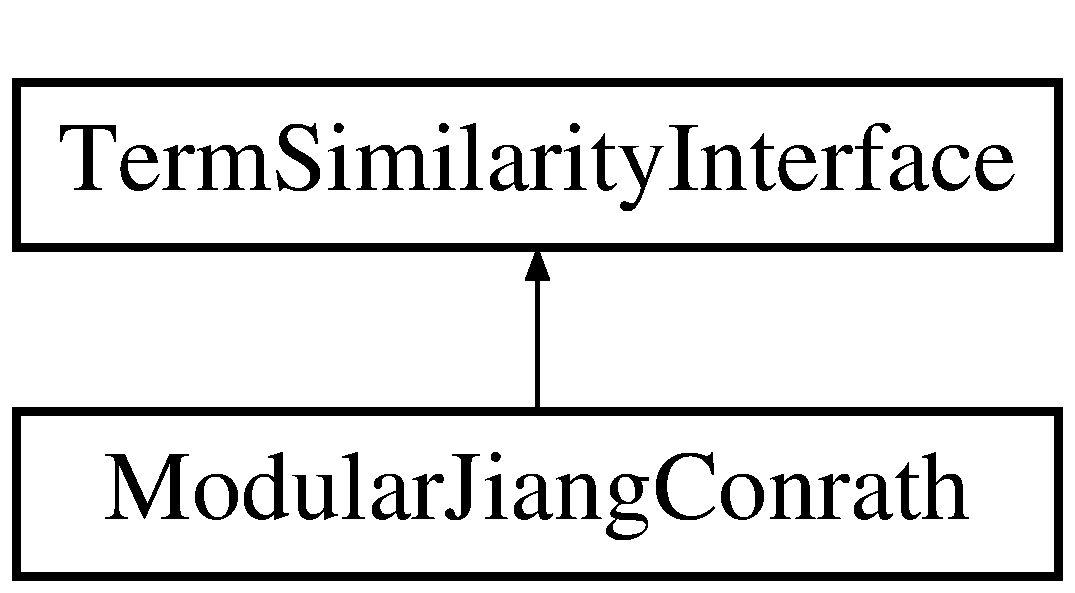
\includegraphics[height=2.000000cm]{classModularJiangConrath}
\end{center}
\end{figure}
\subsection*{Public Member Functions}
\begin{DoxyCompactItemize}
\item 
\hyperlink{classModularJiangConrath_aae432a48629db51d0f0d00a41d592b87}{Modular\+Jiang\+Conrath} (\hyperlink{classSharedInformationInterface}{Shared\+Information\+Interface} $\ast$shared\+Information\+Calculator)
\begin{DoxyCompactList}\small\item\em A constructor. \end{DoxyCompactList}\item 
double \hyperlink{classModularJiangConrath_a4bb41aa1eced9dd47f4f4c7125a223d5}{calculate\+Term\+Similarity} (std\+::string go\+TermA, std\+::string go\+TermB)
\begin{DoxyCompactList}\small\item\em A method for calculating term-\/to-\/term similarity for \hyperlink{namespaceGO}{GO} terms using Lin similarity. \end{DoxyCompactList}\item 
double \hyperlink{classModularJiangConrath_afbcb95c5f87764de5d33188948f1001b}{calculate\+Normalized\+Term\+Similarity} (std\+::string go\+TermA, std\+::string go\+TermB)
\begin{DoxyCompactList}\small\item\em A method for calculating term-\/to-\/term similarity for \hyperlink{namespaceGO}{GO} terms using normalized Lin similarity. \end{DoxyCompactList}\item 
void \hyperlink{classModularJiangConrath_a44a9dae983e696676cb41c8cf8f93cb6}{set\+Shared\+Information\+Calculator} (\hyperlink{classSharedInformationInterface}{Shared\+Information\+Interface} $\ast$new\+Shared\+Information\+Calulator)
\begin{DoxyCompactList}\small\item\em A method to set alternative methods of shared information calculators. \end{DoxyCompactList}\end{DoxyCompactItemize}


\subsection{Detailed Description}
A class to calculate Jiang Conrath similarity between 2 terms. 

This class calculates Jiang Conrath similarity.

Jiang, J. J., \& Conrath, D. W. (1997). Semantic similarity based on corpus statistics and lexical taxonomy. In Proc. of 10th International Conference on Research on Computational Linguistics, Taiwan.

P. W. Lord, R. D. Stevens, A. Brass, and C. A. Goble, \char`\"{}\+Semantic similarity measures as tools for exploring the gene ontology,\char`\"{} Pac Symp Biocomput, pp. 601-\/12, 2003.

distance = I\+C(term\+A) + I\+C(term\+B) -\/ 2$\ast$\+IC(M\+I\+CA) max\+Distance = 2$\ast$\+IC(single annotaiotn) similarity = 1 -\/ distance/max\+Distance (see Lord et al.) 

\subsection{Constructor \& Destructor Documentation}
\index{Modular\+Jiang\+Conrath@{Modular\+Jiang\+Conrath}!Modular\+Jiang\+Conrath@{Modular\+Jiang\+Conrath}}
\index{Modular\+Jiang\+Conrath@{Modular\+Jiang\+Conrath}!Modular\+Jiang\+Conrath@{Modular\+Jiang\+Conrath}}
\subsubsection[{\texorpdfstring{Modular\+Jiang\+Conrath(\+Shared\+Information\+Interface $\ast$shared\+Information\+Calculator)}{ModularJiangConrath(SharedInformationInterface *sharedInformationCalculator)}}]{\setlength{\rightskip}{0pt plus 5cm}Modular\+Jiang\+Conrath\+::\+Modular\+Jiang\+Conrath (
\begin{DoxyParamCaption}
\item[{{\bf Shared\+Information\+Interface} $\ast$}]{shared\+Information\+Calculator}
\end{DoxyParamCaption}
)\hspace{0.3cm}{\ttfamily [inline]}}\hypertarget{classModularJiangConrath_aae432a48629db51d0f0d00a41d592b87}{}\label{classModularJiangConrath_aae432a48629db51d0f0d00a41d592b87}


A constructor. 

Creates the Jiang Conrath simialrity measure using a given shared infromation calculator 

\subsection{Member Function Documentation}
\index{Modular\+Jiang\+Conrath@{Modular\+Jiang\+Conrath}!calculate\+Normalized\+Term\+Similarity@{calculate\+Normalized\+Term\+Similarity}}
\index{calculate\+Normalized\+Term\+Similarity@{calculate\+Normalized\+Term\+Similarity}!Modular\+Jiang\+Conrath@{Modular\+Jiang\+Conrath}}
\subsubsection[{\texorpdfstring{calculate\+Normalized\+Term\+Similarity(std\+::string go\+Term\+A, std\+::string go\+Term\+B)}{calculateNormalizedTermSimilarity(std::string goTermA, std::string goTermB)}}]{\setlength{\rightskip}{0pt plus 5cm}double Modular\+Jiang\+Conrath\+::calculate\+Normalized\+Term\+Similarity (
\begin{DoxyParamCaption}
\item[{std\+::string}]{go\+TermA, }
\item[{std\+::string}]{go\+TermB}
\end{DoxyParamCaption}
)\hspace{0.3cm}{\ttfamily [inline]}, {\ttfamily [virtual]}}\hypertarget{classModularJiangConrath_afbcb95c5f87764de5d33188948f1001b}{}\label{classModularJiangConrath_afbcb95c5f87764de5d33188948f1001b}


A method for calculating term-\/to-\/term similarity for \hyperlink{namespaceGO}{GO} terms using normalized Lin similarity. 

This method returns the Lin similarity. Lin similarity is already normalized 

Implements \hyperlink{classTermSimilarityInterface_aa46b7870c7725faab85ec502a3e5242d}{Term\+Similarity\+Interface}.

\index{Modular\+Jiang\+Conrath@{Modular\+Jiang\+Conrath}!calculate\+Term\+Similarity@{calculate\+Term\+Similarity}}
\index{calculate\+Term\+Similarity@{calculate\+Term\+Similarity}!Modular\+Jiang\+Conrath@{Modular\+Jiang\+Conrath}}
\subsubsection[{\texorpdfstring{calculate\+Term\+Similarity(std\+::string go\+Term\+A, std\+::string go\+Term\+B)}{calculateTermSimilarity(std::string goTermA, std::string goTermB)}}]{\setlength{\rightskip}{0pt plus 5cm}double Modular\+Jiang\+Conrath\+::calculate\+Term\+Similarity (
\begin{DoxyParamCaption}
\item[{std\+::string}]{go\+TermA, }
\item[{std\+::string}]{go\+TermB}
\end{DoxyParamCaption}
)\hspace{0.3cm}{\ttfamily [inline]}, {\ttfamily [virtual]}}\hypertarget{classModularJiangConrath_a4bb41aa1eced9dd47f4f4c7125a223d5}{}\label{classModularJiangConrath_a4bb41aa1eced9dd47f4f4c7125a223d5}


A method for calculating term-\/to-\/term similarity for \hyperlink{namespaceGO}{GO} terms using Lin similarity. 

This method returns the Resnik similarity or the information content of the most informative common ancestor. 

Implements \hyperlink{classTermSimilarityInterface_ae3474adcfcb02faef65ed5e16ef4db47}{Term\+Similarity\+Interface}.

\index{Modular\+Jiang\+Conrath@{Modular\+Jiang\+Conrath}!set\+Shared\+Information\+Calculator@{set\+Shared\+Information\+Calculator}}
\index{set\+Shared\+Information\+Calculator@{set\+Shared\+Information\+Calculator}!Modular\+Jiang\+Conrath@{Modular\+Jiang\+Conrath}}
\subsubsection[{\texorpdfstring{set\+Shared\+Information\+Calculator(\+Shared\+Information\+Interface $\ast$new\+Shared\+Information\+Calulator)}{setSharedInformationCalculator(SharedInformationInterface *newSharedInformationCalulator)}}]{\setlength{\rightskip}{0pt plus 5cm}void Modular\+Jiang\+Conrath\+::set\+Shared\+Information\+Calculator (
\begin{DoxyParamCaption}
\item[{{\bf Shared\+Information\+Interface} $\ast$}]{new\+Shared\+Information\+Calulator}
\end{DoxyParamCaption}
)\hspace{0.3cm}{\ttfamily [inline]}}\hypertarget{classModularJiangConrath_a44a9dae983e696676cb41c8cf8f93cb6}{}\label{classModularJiangConrath_a44a9dae983e696676cb41c8cf8f93cb6}


A method to set alternative methods of shared information calculators. 

This method accepts a new method for calculating the shared information of two terms. 

The documentation for this class was generated from the following file\+:\begin{DoxyCompactItemize}
\item 
ggtk/Modular\+Jiang\+Conrath.\+hpp\end{DoxyCompactItemize}

\hypertarget{classModularLin}{}\section{Modular\+Lin Class Reference}
\label{classModularLin}\index{Modular\+Lin@{Modular\+Lin}}


A class to calculate Lin similarity between 2 terms.  




{\ttfamily \#include $<$ggtk/\+Modular\+Lin.\+hpp$>$}

Inheritance diagram for Modular\+Lin\+:\begin{figure}[H]
\begin{center}
\leavevmode
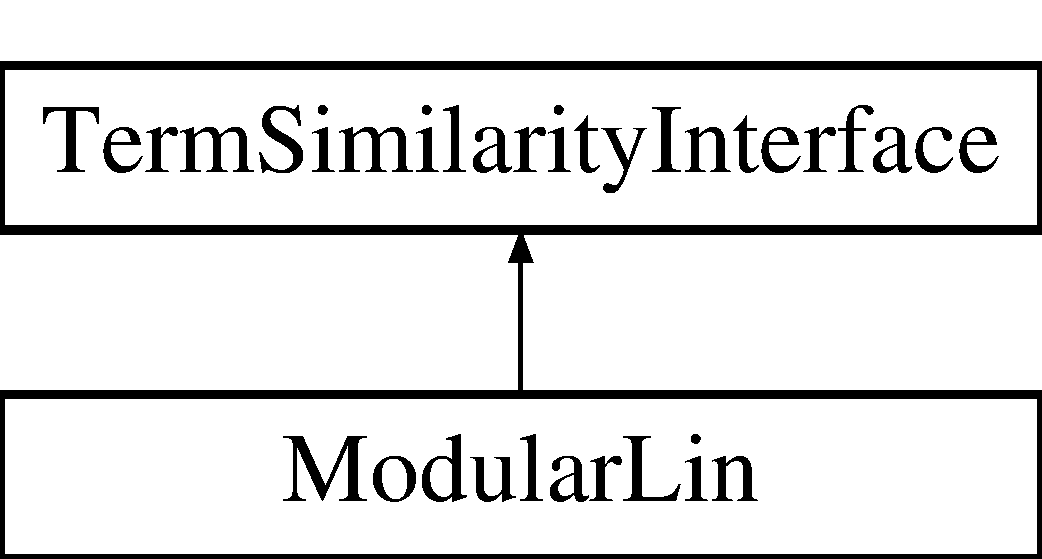
\includegraphics[height=2.000000cm]{classModularLin}
\end{center}
\end{figure}
\subsection*{Public Member Functions}
\begin{DoxyCompactItemize}
\item 
\hyperlink{classModularLin_a1d70b04bb6d75af7d86da15f33bb1732}{Modular\+Lin} (\hyperlink{classSharedInformationInterface}{Shared\+Information\+Interface} $\ast$shared\+Information\+Calculator)
\begin{DoxyCompactList}\small\item\em A constructor. \end{DoxyCompactList}\item 
double \hyperlink{classModularLin_a995ef9e4c53b9e96a32259157416df1b}{calculate\+Term\+Similarity} (std\+::string go\+TermA, std\+::string go\+TermB)
\begin{DoxyCompactList}\small\item\em A method for calculating term-\/to-\/term similarity for \hyperlink{namespaceGO}{GO} terms using Lin similarity. \end{DoxyCompactList}\item 
double \hyperlink{classModularLin_a5c4c590808542669e7ba65b60ea8f707}{calculate\+Normalized\+Term\+Similarity} (std\+::string go\+TermA, std\+::string go\+TermB)
\begin{DoxyCompactList}\small\item\em A method for calculating term-\/to-\/term similarity for \hyperlink{namespaceGO}{GO} terms using normalized Lin similarity. \end{DoxyCompactList}\item 
void \hyperlink{classModularLin_a2730653a908d1d3ae8d379d166906646}{set\+Shared\+Information\+Calculator} (\hyperlink{classSharedInformationInterface}{Shared\+Information\+Interface} $\ast$new\+Shared\+Information\+Calulator)
\begin{DoxyCompactList}\small\item\em A method to set alternative methods of shared information calculators. \end{DoxyCompactList}\end{DoxyCompactItemize}


\subsection{Detailed Description}
A class to calculate Lin similarity between 2 terms. 

This class calculates Lin similarity.

Lin, D. (1998) An information theoretic definition of similarity. In\+: Proc. of the 15th Inernational Conference on Machine Learning. San Franscisco, CA\+: Morgan Kaufman. pp 296-\/304

P. W. Lord, R. D. Stevens, A. Brass, and C. A. Goble, \char`\"{}\+Semantic similarity measures as tools for exploring the gene ontology,\char`\"{} Pac Symp Biocomput, pp. 601-\/12, 2003.

2 $\ast$ I\+C(\+M\+I\+C\+A) / ( I\+C(term\+A) + I\+C(term\+B) ) 

\subsection{Constructor \& Destructor Documentation}
\index{Modular\+Lin@{Modular\+Lin}!Modular\+Lin@{Modular\+Lin}}
\index{Modular\+Lin@{Modular\+Lin}!Modular\+Lin@{Modular\+Lin}}
\subsubsection[{\texorpdfstring{Modular\+Lin(\+Shared\+Information\+Interface $\ast$shared\+Information\+Calculator)}{ModularLin(SharedInformationInterface *sharedInformationCalculator)}}]{\setlength{\rightskip}{0pt plus 5cm}Modular\+Lin\+::\+Modular\+Lin (
\begin{DoxyParamCaption}
\item[{{\bf Shared\+Information\+Interface} $\ast$}]{shared\+Information\+Calculator}
\end{DoxyParamCaption}
)\hspace{0.3cm}{\ttfamily [inline]}}\hypertarget{classModularLin_a1d70b04bb6d75af7d86da15f33bb1732}{}\label{classModularLin_a1d70b04bb6d75af7d86da15f33bb1732}


A constructor. 

Creates the \hyperlink{classLinSimilarity}{Lin\+Similarity} calculator with a particular shared information calculator 

\subsection{Member Function Documentation}
\index{Modular\+Lin@{Modular\+Lin}!calculate\+Normalized\+Term\+Similarity@{calculate\+Normalized\+Term\+Similarity}}
\index{calculate\+Normalized\+Term\+Similarity@{calculate\+Normalized\+Term\+Similarity}!Modular\+Lin@{Modular\+Lin}}
\subsubsection[{\texorpdfstring{calculate\+Normalized\+Term\+Similarity(std\+::string go\+Term\+A, std\+::string go\+Term\+B)}{calculateNormalizedTermSimilarity(std::string goTermA, std::string goTermB)}}]{\setlength{\rightskip}{0pt plus 5cm}double Modular\+Lin\+::calculate\+Normalized\+Term\+Similarity (
\begin{DoxyParamCaption}
\item[{std\+::string}]{go\+TermA, }
\item[{std\+::string}]{go\+TermB}
\end{DoxyParamCaption}
)\hspace{0.3cm}{\ttfamily [inline]}, {\ttfamily [virtual]}}\hypertarget{classModularLin_a5c4c590808542669e7ba65b60ea8f707}{}\label{classModularLin_a5c4c590808542669e7ba65b60ea8f707}


A method for calculating term-\/to-\/term similarity for \hyperlink{namespaceGO}{GO} terms using normalized Lin similarity. 

This method returns the Lin similarity. Lin similarity is already normalized 

Implements \hyperlink{classTermSimilarityInterface_aa46b7870c7725faab85ec502a3e5242d}{Term\+Similarity\+Interface}.

\index{Modular\+Lin@{Modular\+Lin}!calculate\+Term\+Similarity@{calculate\+Term\+Similarity}}
\index{calculate\+Term\+Similarity@{calculate\+Term\+Similarity}!Modular\+Lin@{Modular\+Lin}}
\subsubsection[{\texorpdfstring{calculate\+Term\+Similarity(std\+::string go\+Term\+A, std\+::string go\+Term\+B)}{calculateTermSimilarity(std::string goTermA, std::string goTermB)}}]{\setlength{\rightskip}{0pt plus 5cm}double Modular\+Lin\+::calculate\+Term\+Similarity (
\begin{DoxyParamCaption}
\item[{std\+::string}]{go\+TermA, }
\item[{std\+::string}]{go\+TermB}
\end{DoxyParamCaption}
)\hspace{0.3cm}{\ttfamily [inline]}, {\ttfamily [virtual]}}\hypertarget{classModularLin_a995ef9e4c53b9e96a32259157416df1b}{}\label{classModularLin_a995ef9e4c53b9e96a32259157416df1b}


A method for calculating term-\/to-\/term similarity for \hyperlink{namespaceGO}{GO} terms using Lin similarity. 

This method returns the Resnik similarity or the information content of the most informative common ancestor. 

Implements \hyperlink{classTermSimilarityInterface_ae3474adcfcb02faef65ed5e16ef4db47}{Term\+Similarity\+Interface}.

\index{Modular\+Lin@{Modular\+Lin}!set\+Shared\+Information\+Calculator@{set\+Shared\+Information\+Calculator}}
\index{set\+Shared\+Information\+Calculator@{set\+Shared\+Information\+Calculator}!Modular\+Lin@{Modular\+Lin}}
\subsubsection[{\texorpdfstring{set\+Shared\+Information\+Calculator(\+Shared\+Information\+Interface $\ast$new\+Shared\+Information\+Calulator)}{setSharedInformationCalculator(SharedInformationInterface *newSharedInformationCalulator)}}]{\setlength{\rightskip}{0pt plus 5cm}void Modular\+Lin\+::set\+Shared\+Information\+Calculator (
\begin{DoxyParamCaption}
\item[{{\bf Shared\+Information\+Interface} $\ast$}]{new\+Shared\+Information\+Calulator}
\end{DoxyParamCaption}
)\hspace{0.3cm}{\ttfamily [inline]}}\hypertarget{classModularLin_a2730653a908d1d3ae8d379d166906646}{}\label{classModularLin_a2730653a908d1d3ae8d379d166906646}


A method to set alternative methods of shared information calculators. 

This method accepts a new method for calculating the shared information of two terms. 

The documentation for this class was generated from the following file\+:\begin{DoxyCompactItemize}
\item 
ggtk/Modular\+Lin.\+hpp\end{DoxyCompactItemize}

\hypertarget{classModularResnik}{}\section{Modular\+Resnik Class Reference}
\label{classModularResnik}\index{Modular\+Resnik@{Modular\+Resnik}}


A class to calculate resnik similarity between 2 terms using a shared information interface.  




{\ttfamily \#include $<$ggtk/\+Modular\+Resnik.\+hpp$>$}

Inheritance diagram for Modular\+Resnik\+:\begin{figure}[H]
\begin{center}
\leavevmode
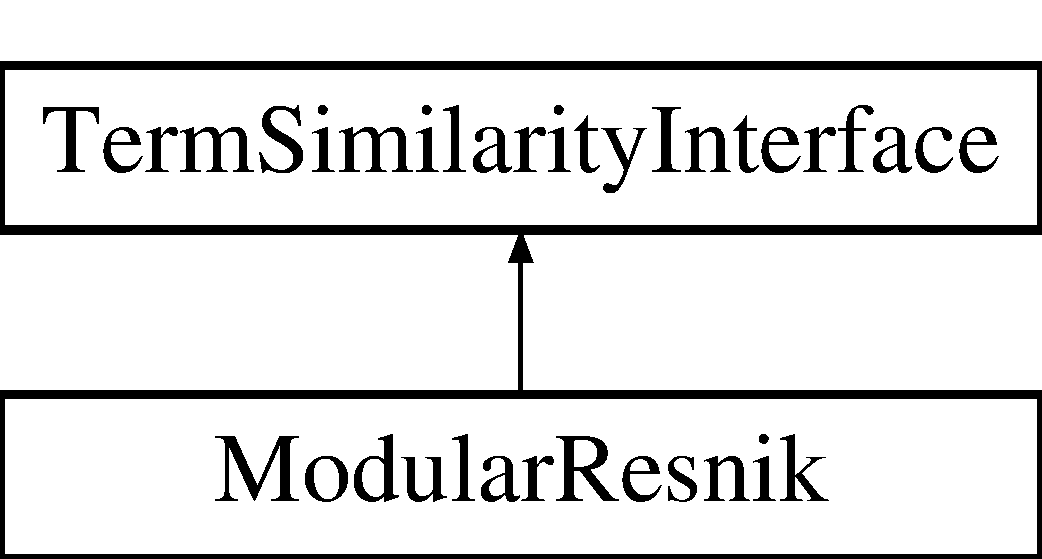
\includegraphics[height=2.000000cm]{classModularResnik}
\end{center}
\end{figure}
\subsection*{Public Member Functions}
\begin{DoxyCompactItemize}
\item 
\hyperlink{classModularResnik_a53d184cbe8caf8222455808b03fdc5c9}{Modular\+Resnik} (\hyperlink{classSharedInformationInterface}{Shared\+Information\+Interface} $\ast$shared\+Information\+Calculator)
\begin{DoxyCompactList}\small\item\em A constructor. \end{DoxyCompactList}\item 
double \hyperlink{classModularResnik_a78b925c1aadb000d1773ffdacad549df}{calculate\+Term\+Similarity} (std\+::string go\+TermA, std\+::string go\+TermB)
\begin{DoxyCompactList}\small\item\em A method for calculating term-\/to-\/term similarity for \hyperlink{namespaceGO}{GO} terms using Resnik similarity. \end{DoxyCompactList}\item 
double \hyperlink{classModularResnik_aba93eb85400287057037d545e5080265}{calculate\+Normalized\+Term\+Similarity} (std\+::string go\+TermA, std\+::string go\+TermB)
\begin{DoxyCompactList}\small\item\em A method for calculating term-\/to-\/term similarity for \hyperlink{namespaceGO}{GO} terms using Normalized Resnik similarity. \end{DoxyCompactList}\item 
void \hyperlink{classModularResnik_ab0402a3be9f5b1e590c50b38e4a7fd39}{set\+Shared\+Information\+Calculator} (\hyperlink{classSharedInformationInterface}{Shared\+Information\+Interface} $\ast$new\+Shared\+Information\+Calulator)
\begin{DoxyCompactList}\small\item\em A constructor. \end{DoxyCompactList}\end{DoxyCompactItemize}


\subsection{Detailed Description}
A class to calculate resnik similarity between 2 terms using a shared information interface. 

This class calculates Resnik similarity. Philip Resnik (1995). \char`\"{}\+Using information content to evaluate semantic similarity in a taxonomy\char`\"{}. In Chris S. Mellish (Ed.). Proceedings of the 14th international joint conference on Artificial intelligence (I\+J\+C\+AI\textquotesingle{}95)

P. W. Lord, R. D. Stevens, A. Brass, and C. A. Goble, \char`\"{}\+Semantic similarity measures as tools for exploring the gene ontology,\char`\"{} Pac Symp Biocomput, pp. 601-\/12, 2003.

maximun information content of all shared ancestors I\+C(\+M\+I\+C\+A) 

\subsection{Constructor \& Destructor Documentation}
\index{Modular\+Resnik@{Modular\+Resnik}!Modular\+Resnik@{Modular\+Resnik}}
\index{Modular\+Resnik@{Modular\+Resnik}!Modular\+Resnik@{Modular\+Resnik}}
\subsubsection[{\texorpdfstring{Modular\+Resnik(\+Shared\+Information\+Interface $\ast$shared\+Information\+Calculator)}{ModularResnik(SharedInformationInterface *sharedInformationCalculator)}}]{\setlength{\rightskip}{0pt plus 5cm}Modular\+Resnik\+::\+Modular\+Resnik (
\begin{DoxyParamCaption}
\item[{{\bf Shared\+Information\+Interface} $\ast$}]{shared\+Information\+Calculator}
\end{DoxyParamCaption}
)\hspace{0.3cm}{\ttfamily [inline]}}\hypertarget{classModularResnik_a53d184cbe8caf8222455808b03fdc5c9}{}\label{classModularResnik_a53d184cbe8caf8222455808b03fdc5c9}


A constructor. 

Creates the default(empty) \hyperlink{classStandardRelationshipPolicy}{Standard\+Relationship\+Policy} 

\subsection{Member Function Documentation}
\index{Modular\+Resnik@{Modular\+Resnik}!calculate\+Normalized\+Term\+Similarity@{calculate\+Normalized\+Term\+Similarity}}
\index{calculate\+Normalized\+Term\+Similarity@{calculate\+Normalized\+Term\+Similarity}!Modular\+Resnik@{Modular\+Resnik}}
\subsubsection[{\texorpdfstring{calculate\+Normalized\+Term\+Similarity(std\+::string go\+Term\+A, std\+::string go\+Term\+B)}{calculateNormalizedTermSimilarity(std::string goTermA, std::string goTermB)}}]{\setlength{\rightskip}{0pt plus 5cm}double Modular\+Resnik\+::calculate\+Normalized\+Term\+Similarity (
\begin{DoxyParamCaption}
\item[{std\+::string}]{go\+TermA, }
\item[{std\+::string}]{go\+TermB}
\end{DoxyParamCaption}
)\hspace{0.3cm}{\ttfamily [inline]}, {\ttfamily [virtual]}}\hypertarget{classModularResnik_aba93eb85400287057037d545e5080265}{}\label{classModularResnik_aba93eb85400287057037d545e5080265}


A method for calculating term-\/to-\/term similarity for \hyperlink{namespaceGO}{GO} terms using Normalized Resnik similarity. 

This method returns the Resnik similarity divided by the maximum possible similarity 

Implements \hyperlink{classTermSimilarityInterface_aa46b7870c7725faab85ec502a3e5242d}{Term\+Similarity\+Interface}.

\index{Modular\+Resnik@{Modular\+Resnik}!calculate\+Term\+Similarity@{calculate\+Term\+Similarity}}
\index{calculate\+Term\+Similarity@{calculate\+Term\+Similarity}!Modular\+Resnik@{Modular\+Resnik}}
\subsubsection[{\texorpdfstring{calculate\+Term\+Similarity(std\+::string go\+Term\+A, std\+::string go\+Term\+B)}{calculateTermSimilarity(std::string goTermA, std::string goTermB)}}]{\setlength{\rightskip}{0pt plus 5cm}double Modular\+Resnik\+::calculate\+Term\+Similarity (
\begin{DoxyParamCaption}
\item[{std\+::string}]{go\+TermA, }
\item[{std\+::string}]{go\+TermB}
\end{DoxyParamCaption}
)\hspace{0.3cm}{\ttfamily [inline]}, {\ttfamily [virtual]}}\hypertarget{classModularResnik_a78b925c1aadb000d1773ffdacad549df}{}\label{classModularResnik_a78b925c1aadb000d1773ffdacad549df}


A method for calculating term-\/to-\/term similarity for \hyperlink{namespaceGO}{GO} terms using Resnik similarity. 

This method returns the Resnik similarity or the information content of the most informative common ancestor. 

Implements \hyperlink{classTermSimilarityInterface_ae3474adcfcb02faef65ed5e16ef4db47}{Term\+Similarity\+Interface}.

\index{Modular\+Resnik@{Modular\+Resnik}!set\+Shared\+Information\+Calculator@{set\+Shared\+Information\+Calculator}}
\index{set\+Shared\+Information\+Calculator@{set\+Shared\+Information\+Calculator}!Modular\+Resnik@{Modular\+Resnik}}
\subsubsection[{\texorpdfstring{set\+Shared\+Information\+Calculator(\+Shared\+Information\+Interface $\ast$new\+Shared\+Information\+Calulator)}{setSharedInformationCalculator(SharedInformationInterface *newSharedInformationCalulator)}}]{\setlength{\rightskip}{0pt plus 5cm}void Modular\+Resnik\+::set\+Shared\+Information\+Calculator (
\begin{DoxyParamCaption}
\item[{{\bf Shared\+Information\+Interface} $\ast$}]{new\+Shared\+Information\+Calulator}
\end{DoxyParamCaption}
)\hspace{0.3cm}{\ttfamily [inline]}}\hypertarget{classModularResnik_ab0402a3be9f5b1e590c50b38e4a7fd39}{}\label{classModularResnik_ab0402a3be9f5b1e590c50b38e4a7fd39}


A constructor. 

Creates the default(empty) \hyperlink{classStandardRelationshipPolicy}{Standard\+Relationship\+Policy} 

The documentation for this class was generated from the following file\+:\begin{DoxyCompactItemize}
\item 
ggtk/Modular\+Resnik.\+hpp\end{DoxyCompactItemize}

\hypertarget{classNCList}{}\section{N\+C\+List Class Reference}
\label{classNCList}\index{N\+C\+List@{N\+C\+List}}


A container class for quickly finding intersections of genomic intervals.  




{\ttfamily \#include $<$ggtk/\+N\+C\+List.\+hpp$>$}

\subsection*{Classes}
\begin{DoxyCompactItemize}
\item 
class \hyperlink{classNCList_1_1NCNode}{N\+C\+Node}
\end{DoxyCompactItemize}
\subsection*{Public Member Functions}
\begin{DoxyCompactItemize}
\item 
\hyperlink{classNCList_ab6c2b7decd70fcde7b54db4e79b64b85}{N\+C\+List} (std\+::vector$<$ \hyperlink{classGenomicRegion}{Genomic\+Region} $>$ \&regions)
\item 
size\+\_\+t \hyperlink{classNCList_a98e796a8e78efec9d019fb4303d4c8f3}{get\+Overlap\+Index} (const \hyperlink{classGenomicRegion}{Genomic\+Region} r)
\item 
size\+\_\+t \hyperlink{classNCList_a3199031fe2904e2cac57a682e07573c5}{get\+Overlap\+Index} (const std\+::pair$<$ size\+\_\+t, size\+\_\+t $>$ p)
\item 
size\+\_\+t \hyperlink{classNCList_a01ce26e143d1edf32caf50d472c1cce3}{get\+Overlap\+Index} (const size\+\_\+t start, const size\+\_\+t end)
\item 
size\+\_\+t \hyperlink{classNCList_a226ca89f140feac5088af4be366bcd58}{get\+Overlap\+Index} (const size\+\_\+t point)
\item 
std\+::vector$<$ \hyperlink{classGenomicRegion}{Genomic\+Region} $>$ \hyperlink{classNCList_af67a0c748ed4e7d095bb6092c1f291fb}{get\+Features} ()
\item 
std\+::vector$<$ \hyperlink{classGenomicRegion}{Genomic\+Region} $>$ \hyperlink{classNCList_acaec79f5de348b5645a856fcde6d58cf}{get\+Features\+In\+Range} (const \hyperlink{classGenomicRegion}{Genomic\+Region} r)
\item 
std\+::vector$<$ \hyperlink{classGenomicRegion}{Genomic\+Region} $>$ \hyperlink{classNCList_aab695768230d12b179699ca8f19f5d4c}{get\+Features\+In\+Range} (const std\+::pair$<$ size\+\_\+t, size\+\_\+t $>$ p)
\item 
std\+::vector$<$ \hyperlink{classGenomicRegion}{Genomic\+Region} $>$ \hyperlink{classNCList_a02b767b23f0007af67174cb2c2e6d92b}{get\+Features\+In\+Range} (const size\+\_\+t start, const size\+\_\+t end)
\item 
std\+::vector$<$ \hyperlink{classGenomicRegion}{Genomic\+Region} $>$ \hyperlink{classNCList_a6de14b47eb6b5c7291f5469609d500f6}{get\+Features\+At} (const size\+\_\+t index)
\item 
size\+\_\+t \hyperlink{classNCList_a4bb83c717bfa1b169f48809a4ed32f2e}{size} ()
\item 
size\+\_\+t \hyperlink{classNCList_a88ba10ba7017497f6912e8f3570239e9}{num\+Features} ()
\item 
std\+::vector$<$ \hyperlink{classNCList_1_1NCNode}{N\+C\+Node} $>$ \hyperlink{classNCList_a4ea0b59d58fcd385adb2fa4e92aae35b}{get\+Nodes} ()
\item 
\hyperlink{classGenomicRegion}{Genomic\+Region} \hyperlink{classNCList_a002aee45aea558b91957c4f282b83565}{get\+Region\+At} (size\+\_\+t i)
\end{DoxyCompactItemize}
\subsection*{Public Attributes}
\begin{DoxyCompactItemize}
\item 
std\+::vector$<$ \hyperlink{classNCList_1_1NCNode}{N\+C\+Node} $>$ \hyperlink{classNCList_a2999e47110bf2e20bb9fd8e8689715e3}{\+\_\+items}
\end{DoxyCompactItemize}


\subsection{Detailed Description}
A container class for quickly finding intersections of genomic intervals. 

This class prepresents an implementation of Nested Containment Lists by Alekseyenko and Lee.

Alekseyenko AV and Lee CJ. Nested Containment List (\hyperlink{classNCList}{N\+C\+List})\+: a new algorithm for accelerating interval query of genome alignment and interval databases. Bioinformatics. 2007 Jun 1;23(11)\+:1386-\/93. Epub 2007 Jan 18. 

\subsection{Constructor \& Destructor Documentation}
\index{N\+C\+List@{N\+C\+List}!N\+C\+List@{N\+C\+List}}
\index{N\+C\+List@{N\+C\+List}!N\+C\+List@{N\+C\+List}}
\subsubsection[{\texorpdfstring{N\+C\+List(std\+::vector$<$ Genomic\+Region $>$ \&regions)}{NCList(std::vector< GenomicRegion > &regions)}}]{\setlength{\rightskip}{0pt plus 5cm}N\+C\+List\+::\+N\+C\+List (
\begin{DoxyParamCaption}
\item[{std\+::vector$<$ {\bf Genomic\+Region} $>$ \&}]{regions}
\end{DoxyParamCaption}
)\hspace{0.3cm}{\ttfamily [inline]}}\hypertarget{classNCList_ab6c2b7decd70fcde7b54db4e79b64b85}{}\label{classNCList_ab6c2b7decd70fcde7b54db4e79b64b85}
Constructor for \hyperlink{classNCList}{N\+C\+List} that performs the work of sorting and inserting intevals into the N\+C\+Nodes. 

\subsection{Member Function Documentation}
\index{N\+C\+List@{N\+C\+List}!get\+Features@{get\+Features}}
\index{get\+Features@{get\+Features}!N\+C\+List@{N\+C\+List}}
\subsubsection[{\texorpdfstring{get\+Features()}{getFeatures()}}]{\setlength{\rightskip}{0pt plus 5cm}std\+::vector$<${\bf Genomic\+Region}$>$ N\+C\+List\+::get\+Features (
\begin{DoxyParamCaption}
{}
\end{DoxyParamCaption}
)\hspace{0.3cm}{\ttfamily [inline]}}\hypertarget{classNCList_af67a0c748ed4e7d095bb6092c1f291fb}{}\label{classNCList_af67a0c748ed4e7d095bb6092c1f291fb}
A method to return all genes as a vector \index{N\+C\+List@{N\+C\+List}!get\+Features\+At@{get\+Features\+At}}
\index{get\+Features\+At@{get\+Features\+At}!N\+C\+List@{N\+C\+List}}
\subsubsection[{\texorpdfstring{get\+Features\+At(const size\+\_\+t index)}{getFeaturesAt(const size_t index)}}]{\setlength{\rightskip}{0pt plus 5cm}std\+::vector$<${\bf Genomic\+Region}$>$ N\+C\+List\+::get\+Features\+At (
\begin{DoxyParamCaption}
\item[{const size\+\_\+t}]{index}
\end{DoxyParamCaption}
)\hspace{0.3cm}{\ttfamily [inline]}}\hypertarget{classNCList_a6de14b47eb6b5c7291f5469609d500f6}{}\label{classNCList_a6de14b47eb6b5c7291f5469609d500f6}
Method to return all genes at a particular index in the list \index{N\+C\+List@{N\+C\+List}!get\+Features\+In\+Range@{get\+Features\+In\+Range}}
\index{get\+Features\+In\+Range@{get\+Features\+In\+Range}!N\+C\+List@{N\+C\+List}}
\subsubsection[{\texorpdfstring{get\+Features\+In\+Range(const Genomic\+Region r)}{getFeaturesInRange(const GenomicRegion r)}}]{\setlength{\rightskip}{0pt plus 5cm}std\+::vector$<${\bf Genomic\+Region}$>$ N\+C\+List\+::get\+Features\+In\+Range (
\begin{DoxyParamCaption}
\item[{const {\bf Genomic\+Region}}]{r}
\end{DoxyParamCaption}
)\hspace{0.3cm}{\ttfamily [inline]}}\hypertarget{classNCList_acaec79f5de348b5645a856fcde6d58cf}{}\label{classNCList_acaec79f5de348b5645a856fcde6d58cf}
Method to return all genes in a given range \index{N\+C\+List@{N\+C\+List}!get\+Features\+In\+Range@{get\+Features\+In\+Range}}
\index{get\+Features\+In\+Range@{get\+Features\+In\+Range}!N\+C\+List@{N\+C\+List}}
\subsubsection[{\texorpdfstring{get\+Features\+In\+Range(const std\+::pair$<$ size\+\_\+t, size\+\_\+t $>$ p)}{getFeaturesInRange(const std::pair< size_t, size_t > p)}}]{\setlength{\rightskip}{0pt plus 5cm}std\+::vector$<${\bf Genomic\+Region}$>$ N\+C\+List\+::get\+Features\+In\+Range (
\begin{DoxyParamCaption}
\item[{const std\+::pair$<$ size\+\_\+t, size\+\_\+t $>$}]{p}
\end{DoxyParamCaption}
)\hspace{0.3cm}{\ttfamily [inline]}}\hypertarget{classNCList_aab695768230d12b179699ca8f19f5d4c}{}\label{classNCList_aab695768230d12b179699ca8f19f5d4c}
Method to return all genes between a start end pair \index{N\+C\+List@{N\+C\+List}!get\+Features\+In\+Range@{get\+Features\+In\+Range}}
\index{get\+Features\+In\+Range@{get\+Features\+In\+Range}!N\+C\+List@{N\+C\+List}}
\subsubsection[{\texorpdfstring{get\+Features\+In\+Range(const size\+\_\+t start, const size\+\_\+t end)}{getFeaturesInRange(const size_t start, const size_t end)}}]{\setlength{\rightskip}{0pt plus 5cm}std\+::vector$<${\bf Genomic\+Region}$>$ N\+C\+List\+::get\+Features\+In\+Range (
\begin{DoxyParamCaption}
\item[{const size\+\_\+t}]{start, }
\item[{const size\+\_\+t}]{end}
\end{DoxyParamCaption}
)\hspace{0.3cm}{\ttfamily [inline]}}\hypertarget{classNCList_a02b767b23f0007af67174cb2c2e6d92b}{}\label{classNCList_a02b767b23f0007af67174cb2c2e6d92b}
Method to return all genes between a start end interval \index{N\+C\+List@{N\+C\+List}!get\+Nodes@{get\+Nodes}}
\index{get\+Nodes@{get\+Nodes}!N\+C\+List@{N\+C\+List}}
\subsubsection[{\texorpdfstring{get\+Nodes()}{getNodes()}}]{\setlength{\rightskip}{0pt plus 5cm}std\+::vector$<${\bf N\+C\+Node}$>$ N\+C\+List\+::get\+Nodes (
\begin{DoxyParamCaption}
{}
\end{DoxyParamCaption}
)\hspace{0.3cm}{\ttfamily [inline]}}\hypertarget{classNCList_a4ea0b59d58fcd385adb2fa4e92aae35b}{}\label{classNCList_a4ea0b59d58fcd385adb2fa4e92aae35b}
return the vector of N\+C\+Nodes \index{N\+C\+List@{N\+C\+List}!get\+Overlap\+Index@{get\+Overlap\+Index}}
\index{get\+Overlap\+Index@{get\+Overlap\+Index}!N\+C\+List@{N\+C\+List}}
\subsubsection[{\texorpdfstring{get\+Overlap\+Index(const Genomic\+Region r)}{getOverlapIndex(const GenomicRegion r)}}]{\setlength{\rightskip}{0pt plus 5cm}size\+\_\+t N\+C\+List\+::get\+Overlap\+Index (
\begin{DoxyParamCaption}
\item[{const {\bf Genomic\+Region}}]{r}
\end{DoxyParamCaption}
)\hspace{0.3cm}{\ttfamily [inline]}}\hypertarget{classNCList_a98e796a8e78efec9d019fb4303d4c8f3}{}\label{classNCList_a98e796a8e78efec9d019fb4303d4c8f3}
Get the list index of the overlapped region \index{N\+C\+List@{N\+C\+List}!get\+Overlap\+Index@{get\+Overlap\+Index}}
\index{get\+Overlap\+Index@{get\+Overlap\+Index}!N\+C\+List@{N\+C\+List}}
\subsubsection[{\texorpdfstring{get\+Overlap\+Index(const std\+::pair$<$ size\+\_\+t, size\+\_\+t $>$ p)}{getOverlapIndex(const std::pair< size_t, size_t > p)}}]{\setlength{\rightskip}{0pt plus 5cm}size\+\_\+t N\+C\+List\+::get\+Overlap\+Index (
\begin{DoxyParamCaption}
\item[{const std\+::pair$<$ size\+\_\+t, size\+\_\+t $>$}]{p}
\end{DoxyParamCaption}
)\hspace{0.3cm}{\ttfamily [inline]}}\hypertarget{classNCList_a3199031fe2904e2cac57a682e07573c5}{}\label{classNCList_a3199031fe2904e2cac57a682e07573c5}
Get the list index of the overlapped start end pair \index{N\+C\+List@{N\+C\+List}!get\+Overlap\+Index@{get\+Overlap\+Index}}
\index{get\+Overlap\+Index@{get\+Overlap\+Index}!N\+C\+List@{N\+C\+List}}
\subsubsection[{\texorpdfstring{get\+Overlap\+Index(const size\+\_\+t start, const size\+\_\+t end)}{getOverlapIndex(const size_t start, const size_t end)}}]{\setlength{\rightskip}{0pt plus 5cm}size\+\_\+t N\+C\+List\+::get\+Overlap\+Index (
\begin{DoxyParamCaption}
\item[{const size\+\_\+t}]{start, }
\item[{const size\+\_\+t}]{end}
\end{DoxyParamCaption}
)\hspace{0.3cm}{\ttfamily [inline]}}\hypertarget{classNCList_a01ce26e143d1edf32caf50d472c1cce3}{}\label{classNCList_a01ce26e143d1edf32caf50d472c1cce3}
Get the list index of the overlapped start end interval \index{N\+C\+List@{N\+C\+List}!get\+Overlap\+Index@{get\+Overlap\+Index}}
\index{get\+Overlap\+Index@{get\+Overlap\+Index}!N\+C\+List@{N\+C\+List}}
\subsubsection[{\texorpdfstring{get\+Overlap\+Index(const size\+\_\+t point)}{getOverlapIndex(const size_t point)}}]{\setlength{\rightskip}{0pt plus 5cm}size\+\_\+t N\+C\+List\+::get\+Overlap\+Index (
\begin{DoxyParamCaption}
\item[{const size\+\_\+t}]{point}
\end{DoxyParamCaption}
)\hspace{0.3cm}{\ttfamily [inline]}}\hypertarget{classNCList_a226ca89f140feac5088af4be366bcd58}{}\label{classNCList_a226ca89f140feac5088af4be366bcd58}
Get the list index of the overlapped coordinate \index{N\+C\+List@{N\+C\+List}!get\+Region\+At@{get\+Region\+At}}
\index{get\+Region\+At@{get\+Region\+At}!N\+C\+List@{N\+C\+List}}
\subsubsection[{\texorpdfstring{get\+Region\+At(size\+\_\+t i)}{getRegionAt(size_t i)}}]{\setlength{\rightskip}{0pt plus 5cm}{\bf Genomic\+Region} N\+C\+List\+::get\+Region\+At (
\begin{DoxyParamCaption}
\item[{size\+\_\+t}]{i}
\end{DoxyParamCaption}
)\hspace{0.3cm}{\ttfamily [inline]}}\hypertarget{classNCList_a002aee45aea558b91957c4f282b83565}{}\label{classNCList_a002aee45aea558b91957c4f282b83565}
returns the top level region at an index i \index{N\+C\+List@{N\+C\+List}!num\+Features@{num\+Features}}
\index{num\+Features@{num\+Features}!N\+C\+List@{N\+C\+List}}
\subsubsection[{\texorpdfstring{num\+Features()}{numFeatures()}}]{\setlength{\rightskip}{0pt plus 5cm}size\+\_\+t N\+C\+List\+::num\+Features (
\begin{DoxyParamCaption}
{}
\end{DoxyParamCaption}
)\hspace{0.3cm}{\ttfamily [inline]}}\hypertarget{classNCList_a88ba10ba7017497f6912e8f3570239e9}{}\label{classNCList_a88ba10ba7017497f6912e8f3570239e9}
num\+Features returns number of all genes/features \index{N\+C\+List@{N\+C\+List}!size@{size}}
\index{size@{size}!N\+C\+List@{N\+C\+List}}
\subsubsection[{\texorpdfstring{size()}{size()}}]{\setlength{\rightskip}{0pt plus 5cm}size\+\_\+t N\+C\+List\+::size (
\begin{DoxyParamCaption}
{}
\end{DoxyParamCaption}
)\hspace{0.3cm}{\ttfamily [inline]}}\hypertarget{classNCList_a4bb83c717bfa1b169f48809a4ed32f2e}{}\label{classNCList_a4bb83c717bfa1b169f48809a4ed32f2e}
size returns number of top level nodes 

\subsection{Member Data Documentation}
\index{N\+C\+List@{N\+C\+List}!\+\_\+items@{\+\_\+items}}
\index{\+\_\+items@{\+\_\+items}!N\+C\+List@{N\+C\+List}}
\subsubsection[{\texorpdfstring{\+\_\+items}{_items}}]{\setlength{\rightskip}{0pt plus 5cm}std\+::vector$<${\bf N\+C\+Node}$>$ N\+C\+List\+::\+\_\+items}\hypertarget{classNCList_a2999e47110bf2e20bb9fd8e8689715e3}{}\label{classNCList_a2999e47110bf2e20bb9fd8e8689715e3}
List of N\+C\+Nodes as a vector 

The documentation for this class was generated from the following file\+:\begin{DoxyCompactItemize}
\item 
ggtk/N\+C\+List.\+hpp\end{DoxyCompactItemize}

\hypertarget{classNCList_1_1NCNode}{}\section{N\+C\+List\+:\+:N\+C\+Node Class Reference}
\label{classNCList_1_1NCNode}\index{N\+C\+List\+::\+N\+C\+Node@{N\+C\+List\+::\+N\+C\+Node}}


{\ttfamily \#include $<$ggtk/\+N\+C\+List.\+hpp$>$}

\subsection*{Public Member Functions}
\begin{DoxyCompactItemize}
\item 
\hyperlink{classNCList_1_1NCNode_af213aa74a3ce198f18f85d56135e927c}{N\+C\+Node} (\hyperlink{classGenomicRegion}{Genomic\+Region} region, std\+::vector$<$ \hyperlink{classGenomicRegion}{Genomic\+Region} $>$ \&containments)
\item 
bool \hyperlink{classNCList_1_1NCNode_a171e5700a93bd6fe87cc19201b51c511}{contains} (const \hyperlink{classGenomicRegion}{Genomic\+Region} g)
\item 
bool \hyperlink{classNCList_1_1NCNode_aed822cb1840061636984d861a2bf6dc1}{contains} (const std\+::pair$<$ size\+\_\+t, size\+\_\+t $>$ p)
\item 
bool \hyperlink{classNCList_1_1NCNode_a7a1dd138ac17fefb6372428d7368fc2f}{contains} (const size\+\_\+t start, const size\+\_\+t end)
\item 
bool \hyperlink{classNCList_1_1NCNode_a321a463ec67ae56320e292684ccf4f05}{contains} (const size\+\_\+t point)
\item 
bool \hyperlink{classNCList_1_1NCNode_a08dc4cd04cd5f055c795e14015fe99d5}{overlaps} (const \hyperlink{classGenomicRegion}{Genomic\+Region} g)
\item 
bool \hyperlink{classNCList_1_1NCNode_adfcf156f611082e8a878cac5144d57f6}{overlaps} (const std\+::pair$<$ size\+\_\+t, size\+\_\+t $>$ p)
\item 
bool \hyperlink{classNCList_1_1NCNode_a480672401a51f10fced603acbd913823}{overlaps} (const size\+\_\+t start, const size\+\_\+t end)
\item 
\hyperlink{classGenomicRegion}{Genomic\+Region} \hyperlink{classNCList_1_1NCNode_a1f892f4b4baea2b6d36b8eb2e92c8181}{get\+Region} ()
\end{DoxyCompactItemize}
\subsection*{Public Attributes}
\begin{DoxyCompactItemize}
\item 
\hyperlink{classGenomicRegion}{Genomic\+Region} \hyperlink{classNCList_1_1NCNode_a369bc4997b8d3ff5c9c5951bd25ae52a}{\+\_\+region}
\item 
\hyperlink{classNCList}{N\+C\+List} $\ast$ \hyperlink{classNCList_1_1NCNode_a112ccb41d149a0b9f9ee3e7d10267f48}{\+\_\+containments}
\end{DoxyCompactItemize}


\subsection{Detailed Description}
Data structure \hyperlink{classNCList_1_1NCNode}{N\+C\+Node}, \hyperlink{classNCList}{N\+C\+List} = List of N\+C\+Nodes 

\subsection{Constructor \& Destructor Documentation}
\index{N\+C\+List\+::\+N\+C\+Node@{N\+C\+List\+::\+N\+C\+Node}!N\+C\+Node@{N\+C\+Node}}
\index{N\+C\+Node@{N\+C\+Node}!N\+C\+List\+::\+N\+C\+Node@{N\+C\+List\+::\+N\+C\+Node}}
\subsubsection[{\texorpdfstring{N\+C\+Node(\+Genomic\+Region region, std\+::vector$<$ Genomic\+Region $>$ \&containments)}{NCNode(GenomicRegion region, std::vector< GenomicRegion > &containments)}}]{\setlength{\rightskip}{0pt plus 5cm}N\+C\+List\+::\+N\+C\+Node\+::\+N\+C\+Node (
\begin{DoxyParamCaption}
\item[{{\bf Genomic\+Region}}]{region, }
\item[{std\+::vector$<$ {\bf Genomic\+Region} $>$ \&}]{containments}
\end{DoxyParamCaption}
)\hspace{0.3cm}{\ttfamily [inline]}}\hypertarget{classNCList_1_1NCNode_af213aa74a3ce198f18f85d56135e927c}{}\label{classNCList_1_1NCNode_af213aa74a3ce198f18f85d56135e927c}
Node Constructor Most of the work done by \hyperlink{classNCList}{N\+C\+List} Constructor 

\subsection{Member Function Documentation}
\index{N\+C\+List\+::\+N\+C\+Node@{N\+C\+List\+::\+N\+C\+Node}!contains@{contains}}
\index{contains@{contains}!N\+C\+List\+::\+N\+C\+Node@{N\+C\+List\+::\+N\+C\+Node}}
\subsubsection[{\texorpdfstring{contains(const Genomic\+Region g)}{contains(const GenomicRegion g)}}]{\setlength{\rightskip}{0pt plus 5cm}bool N\+C\+List\+::\+N\+C\+Node\+::contains (
\begin{DoxyParamCaption}
\item[{const {\bf Genomic\+Region}}]{g}
\end{DoxyParamCaption}
)\hspace{0.3cm}{\ttfamily [inline]}}\hypertarget{classNCList_1_1NCNode_a171e5700a93bd6fe87cc19201b51c511}{}\label{classNCList_1_1NCNode_a171e5700a93bd6fe87cc19201b51c511}
contains a Genomic Region Overloaded methods to check for containment or overlap

Contianment $\vert$-\/-\/-\/-\/-\/-\/-\/-\/-\/-\/-\/-\/-\/-\/-\/-\/-\/-\/-\/-\/-\/-\/-\/-\/-\/---$\vert$ $\vert$-\/-\/-\/-\/-\/-\/-\/-\/-\/-\/-\/-\/-\/-\/-\/---$\vert$ \index{N\+C\+List\+::\+N\+C\+Node@{N\+C\+List\+::\+N\+C\+Node}!contains@{contains}}
\index{contains@{contains}!N\+C\+List\+::\+N\+C\+Node@{N\+C\+List\+::\+N\+C\+Node}}
\subsubsection[{\texorpdfstring{contains(const std\+::pair$<$ size\+\_\+t, size\+\_\+t $>$ p)}{contains(const std::pair< size_t, size_t > p)}}]{\setlength{\rightskip}{0pt plus 5cm}bool N\+C\+List\+::\+N\+C\+Node\+::contains (
\begin{DoxyParamCaption}
\item[{const std\+::pair$<$ size\+\_\+t, size\+\_\+t $>$}]{p}
\end{DoxyParamCaption}
)\hspace{0.3cm}{\ttfamily [inline]}}\hypertarget{classNCList_1_1NCNode_aed822cb1840061636984d861a2bf6dc1}{}\label{classNCList_1_1NCNode_aed822cb1840061636984d861a2bf6dc1}
contains a start end pair \index{N\+C\+List\+::\+N\+C\+Node@{N\+C\+List\+::\+N\+C\+Node}!contains@{contains}}
\index{contains@{contains}!N\+C\+List\+::\+N\+C\+Node@{N\+C\+List\+::\+N\+C\+Node}}
\subsubsection[{\texorpdfstring{contains(const size\+\_\+t start, const size\+\_\+t end)}{contains(const size_t start, const size_t end)}}]{\setlength{\rightskip}{0pt plus 5cm}bool N\+C\+List\+::\+N\+C\+Node\+::contains (
\begin{DoxyParamCaption}
\item[{const size\+\_\+t}]{start, }
\item[{const size\+\_\+t}]{end}
\end{DoxyParamCaption}
)\hspace{0.3cm}{\ttfamily [inline]}}\hypertarget{classNCList_1_1NCNode_a7a1dd138ac17fefb6372428d7368fc2f}{}\label{classNCList_1_1NCNode_a7a1dd138ac17fefb6372428d7368fc2f}
contains start and end interval \index{N\+C\+List\+::\+N\+C\+Node@{N\+C\+List\+::\+N\+C\+Node}!contains@{contains}}
\index{contains@{contains}!N\+C\+List\+::\+N\+C\+Node@{N\+C\+List\+::\+N\+C\+Node}}
\subsubsection[{\texorpdfstring{contains(const size\+\_\+t point)}{contains(const size_t point)}}]{\setlength{\rightskip}{0pt plus 5cm}bool N\+C\+List\+::\+N\+C\+Node\+::contains (
\begin{DoxyParamCaption}
\item[{const size\+\_\+t}]{point}
\end{DoxyParamCaption}
)\hspace{0.3cm}{\ttfamily [inline]}}\hypertarget{classNCList_1_1NCNode_a321a463ec67ae56320e292684ccf4f05}{}\label{classNCList_1_1NCNode_a321a463ec67ae56320e292684ccf4f05}
contains a single coordinate \index{N\+C\+List\+::\+N\+C\+Node@{N\+C\+List\+::\+N\+C\+Node}!get\+Region@{get\+Region}}
\index{get\+Region@{get\+Region}!N\+C\+List\+::\+N\+C\+Node@{N\+C\+List\+::\+N\+C\+Node}}
\subsubsection[{\texorpdfstring{get\+Region()}{getRegion()}}]{\setlength{\rightskip}{0pt plus 5cm}{\bf Genomic\+Region} N\+C\+List\+::\+N\+C\+Node\+::get\+Region (
\begin{DoxyParamCaption}
{}
\end{DoxyParamCaption}
)\hspace{0.3cm}{\ttfamily [inline]}}\hypertarget{classNCList_1_1NCNode_a1f892f4b4baea2b6d36b8eb2e92c8181}{}\label{classNCList_1_1NCNode_a1f892f4b4baea2b6d36b8eb2e92c8181}
get the current region \index{N\+C\+List\+::\+N\+C\+Node@{N\+C\+List\+::\+N\+C\+Node}!overlaps@{overlaps}}
\index{overlaps@{overlaps}!N\+C\+List\+::\+N\+C\+Node@{N\+C\+List\+::\+N\+C\+Node}}
\subsubsection[{\texorpdfstring{overlaps(const Genomic\+Region g)}{overlaps(const GenomicRegion g)}}]{\setlength{\rightskip}{0pt plus 5cm}bool N\+C\+List\+::\+N\+C\+Node\+::overlaps (
\begin{DoxyParamCaption}
\item[{const {\bf Genomic\+Region}}]{g}
\end{DoxyParamCaption}
)\hspace{0.3cm}{\ttfamily [inline]}}\hypertarget{classNCList_1_1NCNode_a08dc4cd04cd5f055c795e14015fe99d5}{}\label{classNCList_1_1NCNode_a08dc4cd04cd5f055c795e14015fe99d5}
overlaps a genomic region

Overlap $\vert$-\/-\/-\/-\/-\/-\/-\/-\/-\/-\/-\/-\/-\/-\/-\/-\/-\/-\/-\/---$\vert$ $\vert$-\/-\/-\/-\/-\/-\/---$\vert$ or $\vert$-\/-\/-\/-\/-\/-\/-\/-\/---$\vert$ \index{N\+C\+List\+::\+N\+C\+Node@{N\+C\+List\+::\+N\+C\+Node}!overlaps@{overlaps}}
\index{overlaps@{overlaps}!N\+C\+List\+::\+N\+C\+Node@{N\+C\+List\+::\+N\+C\+Node}}
\subsubsection[{\texorpdfstring{overlaps(const std\+::pair$<$ size\+\_\+t, size\+\_\+t $>$ p)}{overlaps(const std::pair< size_t, size_t > p)}}]{\setlength{\rightskip}{0pt plus 5cm}bool N\+C\+List\+::\+N\+C\+Node\+::overlaps (
\begin{DoxyParamCaption}
\item[{const std\+::pair$<$ size\+\_\+t, size\+\_\+t $>$}]{p}
\end{DoxyParamCaption}
)\hspace{0.3cm}{\ttfamily [inline]}}\hypertarget{classNCList_1_1NCNode_adfcf156f611082e8a878cac5144d57f6}{}\label{classNCList_1_1NCNode_adfcf156f611082e8a878cac5144d57f6}
overlaps a start end pair \index{N\+C\+List\+::\+N\+C\+Node@{N\+C\+List\+::\+N\+C\+Node}!overlaps@{overlaps}}
\index{overlaps@{overlaps}!N\+C\+List\+::\+N\+C\+Node@{N\+C\+List\+::\+N\+C\+Node}}
\subsubsection[{\texorpdfstring{overlaps(const size\+\_\+t start, const size\+\_\+t end)}{overlaps(const size_t start, const size_t end)}}]{\setlength{\rightskip}{0pt plus 5cm}bool N\+C\+List\+::\+N\+C\+Node\+::overlaps (
\begin{DoxyParamCaption}
\item[{const size\+\_\+t}]{start, }
\item[{const size\+\_\+t}]{end}
\end{DoxyParamCaption}
)\hspace{0.3cm}{\ttfamily [inline]}}\hypertarget{classNCList_1_1NCNode_a480672401a51f10fced603acbd913823}{}\label{classNCList_1_1NCNode_a480672401a51f10fced603acbd913823}
overlaps a start and end interval 

\subsection{Member Data Documentation}
\index{N\+C\+List\+::\+N\+C\+Node@{N\+C\+List\+::\+N\+C\+Node}!\+\_\+containments@{\+\_\+containments}}
\index{\+\_\+containments@{\+\_\+containments}!N\+C\+List\+::\+N\+C\+Node@{N\+C\+List\+::\+N\+C\+Node}}
\subsubsection[{\texorpdfstring{\+\_\+containments}{_containments}}]{\setlength{\rightskip}{0pt plus 5cm}{\bf N\+C\+List}$\ast$ N\+C\+List\+::\+N\+C\+Node\+::\+\_\+containments}\hypertarget{classNCList_1_1NCNode_a112ccb41d149a0b9f9ee3e7d10267f48}{}\label{classNCList_1_1NCNode_a112ccb41d149a0b9f9ee3e7d10267f48}
List of all regions completely contained by the top level regions interval. \index{N\+C\+List\+::\+N\+C\+Node@{N\+C\+List\+::\+N\+C\+Node}!\+\_\+region@{\+\_\+region}}
\index{\+\_\+region@{\+\_\+region}!N\+C\+List\+::\+N\+C\+Node@{N\+C\+List\+::\+N\+C\+Node}}
\subsubsection[{\texorpdfstring{\+\_\+region}{_region}}]{\setlength{\rightskip}{0pt plus 5cm}{\bf Genomic\+Region} N\+C\+List\+::\+N\+C\+Node\+::\+\_\+region}\hypertarget{classNCList_1_1NCNode_a369bc4997b8d3ff5c9c5951bd25ae52a}{}\label{classNCList_1_1NCNode_a369bc4997b8d3ff5c9c5951bd25ae52a}
Top level region interval. 

The documentation for this class was generated from the following file\+:\begin{DoxyCompactItemize}
\item 
ggtk/N\+C\+List.\+hpp\end{DoxyCompactItemize}

\hypertarget{classPekarStaabSimilarity}{}\section{Pekar\+Staab\+Similarity Class Reference}
\label{classPekarStaabSimilarity}\index{Pekar\+Staab\+Similarity@{Pekar\+Staab\+Similarity}}


A class to calculate Pekar\+Staab similarity between 2 terms.  




{\ttfamily \#include $<$ggtk/\+Pekar\+Staab\+Similarity.\+hpp$>$}

Inheritance diagram for Pekar\+Staab\+Similarity\+:\begin{figure}[H]
\begin{center}
\leavevmode
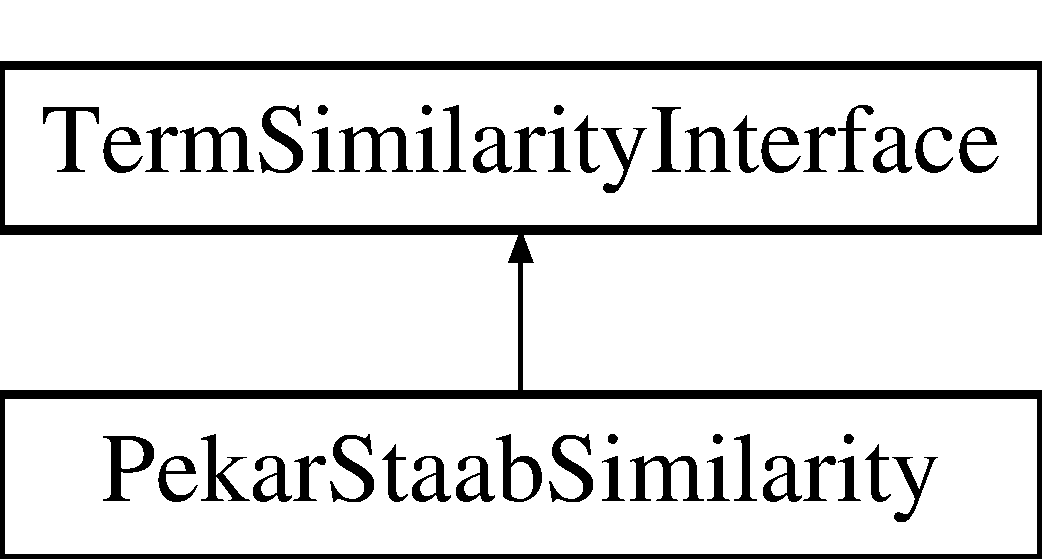
\includegraphics[height=2.000000cm]{classPekarStaabSimilarity}
\end{center}
\end{figure}
\subsection*{Public Member Functions}
\begin{DoxyCompactItemize}
\item 
\hyperlink{classPekarStaabSimilarity_a8da126a2d3dc923dd1749e2f395d41cf}{Pekar\+Staab\+Similarity} (\hyperlink{classGoGraph}{Go\+Graph} $\ast$go\+Graph, \hyperlink{classTermDepthMap}{Term\+Depth\+Map} \&ic\+Map)
\begin{DoxyCompactList}\small\item\em A constructor. \end{DoxyCompactList}\item 
double \hyperlink{classPekarStaabSimilarity_a56bb39dcebcf8909f2006d0698f29211}{calculate\+Term\+Similarity} (std\+::string go\+TermA, std\+::string go\+TermB)
\begin{DoxyCompactList}\small\item\em A method for calculating term-\/to-\/term similarity for \hyperlink{namespaceGO}{GO} terms using Pekar Staab similarity. \end{DoxyCompactList}\item 
double \hyperlink{classPekarStaabSimilarity_a2de7c29ad8e24467c6b66862320953a1}{calculate\+Normalized\+Term\+Similarity} (std\+::string go\+TermA, std\+::string go\+TermB)
\begin{DoxyCompactList}\small\item\em A method for calculating term-\/to-\/term similarity for \hyperlink{namespaceGO}{GO} terms using Normalized Pekar Staab similarity. \end{DoxyCompactList}\item 
std\+::string \hyperlink{classPekarStaabSimilarity_aef5d3e6c69bcd7f614092f342ce624c9}{get\+L\+CA} (boost\+::unordered\+\_\+set$<$ std\+::string $>$ \&ancestorsA, boost\+::unordered\+\_\+set$<$ std\+::string $>$ \&ancestorsB)
\begin{DoxyCompactList}\small\item\em A method for calculating the least common ancestor. \end{DoxyCompactList}\end{DoxyCompactItemize}


\subsection{Detailed Description}
A class to calculate Pekar\+Staab similarity between 2 terms. 

This class calculates Pekar Staab similarity.

V. Pekar and S. Staab, \char`\"{}\+Taxonomy learning\+: factoring the structure 
 of a taxonomy into a semantic classification decision,\char`\"{} in Proc. of 19th International Conference on Computational Linguistics. Morristown NJ U\+SA\+: Association for Computational Linguistics, pp. 1-\/7, 2002.

H. Yu, L. Gao, K. Tu, and Z. Guo, \char`\"{}\+Broadly predicting specific gene 
 functions with expression similarity and taxonomy similarity,\char`\"{} Gene, vol. 352, pp. 75-\/81, Jun 6 2005.

lowest common ancestor (L\+CA) Graph\+Dist(\+L\+C\+A,root)/(Graph\+Dist(a,\+L\+C\+A)+\+Graph\+Dist(b,L\+CA)+\+Graph\+Dist(L\+CA,root)) 

\subsection{Constructor \& Destructor Documentation}
\index{Pekar\+Staab\+Similarity@{Pekar\+Staab\+Similarity}!Pekar\+Staab\+Similarity@{Pekar\+Staab\+Similarity}}
\index{Pekar\+Staab\+Similarity@{Pekar\+Staab\+Similarity}!Pekar\+Staab\+Similarity@{Pekar\+Staab\+Similarity}}
\subsubsection[{\texorpdfstring{Pekar\+Staab\+Similarity(\+Go\+Graph $\ast$go\+Graph, Term\+Depth\+Map \&ic\+Map)}{PekarStaabSimilarity(GoGraph *goGraph, TermDepthMap &icMap)}}]{\setlength{\rightskip}{0pt plus 5cm}Pekar\+Staab\+Similarity\+::\+Pekar\+Staab\+Similarity (
\begin{DoxyParamCaption}
\item[{{\bf Go\+Graph} $\ast$}]{go\+Graph, }
\item[{{\bf Term\+Depth\+Map} \&}]{ic\+Map}
\end{DoxyParamCaption}
)\hspace{0.3cm}{\ttfamily [inline]}}\hypertarget{classPekarStaabSimilarity_a8da126a2d3dc923dd1749e2f395d41cf}{}\label{classPekarStaabSimilarity_a8da126a2d3dc923dd1749e2f395d41cf}


A constructor. 

Creates the default(empty) \hyperlink{classStandardRelationshipPolicy}{Standard\+Relationship\+Policy} 

\subsection{Member Function Documentation}
\index{Pekar\+Staab\+Similarity@{Pekar\+Staab\+Similarity}!calculate\+Normalized\+Term\+Similarity@{calculate\+Normalized\+Term\+Similarity}}
\index{calculate\+Normalized\+Term\+Similarity@{calculate\+Normalized\+Term\+Similarity}!Pekar\+Staab\+Similarity@{Pekar\+Staab\+Similarity}}
\subsubsection[{\texorpdfstring{calculate\+Normalized\+Term\+Similarity(std\+::string go\+Term\+A, std\+::string go\+Term\+B)}{calculateNormalizedTermSimilarity(std::string goTermA, std::string goTermB)}}]{\setlength{\rightskip}{0pt plus 5cm}double Pekar\+Staab\+Similarity\+::calculate\+Normalized\+Term\+Similarity (
\begin{DoxyParamCaption}
\item[{std\+::string}]{go\+TermA, }
\item[{std\+::string}]{go\+TermB}
\end{DoxyParamCaption}
)\hspace{0.3cm}{\ttfamily [inline]}, {\ttfamily [virtual]}}\hypertarget{classPekarStaabSimilarity_a2de7c29ad8e24467c6b66862320953a1}{}\label{classPekarStaabSimilarity_a2de7c29ad8e24467c6b66862320953a1}


A method for calculating term-\/to-\/term similarity for \hyperlink{namespaceGO}{GO} terms using Normalized Pekar Staab similarity. 

This method returns the Pekar\+Staab similarity scaled between 0 and 1 \mbox{[}0,1\mbox{]} inclusive 

Implements \hyperlink{classTermSimilarityInterface_aa46b7870c7725faab85ec502a3e5242d}{Term\+Similarity\+Interface}.

\index{Pekar\+Staab\+Similarity@{Pekar\+Staab\+Similarity}!calculate\+Term\+Similarity@{calculate\+Term\+Similarity}}
\index{calculate\+Term\+Similarity@{calculate\+Term\+Similarity}!Pekar\+Staab\+Similarity@{Pekar\+Staab\+Similarity}}
\subsubsection[{\texorpdfstring{calculate\+Term\+Similarity(std\+::string go\+Term\+A, std\+::string go\+Term\+B)}{calculateTermSimilarity(std::string goTermA, std::string goTermB)}}]{\setlength{\rightskip}{0pt plus 5cm}double Pekar\+Staab\+Similarity\+::calculate\+Term\+Similarity (
\begin{DoxyParamCaption}
\item[{std\+::string}]{go\+TermA, }
\item[{std\+::string}]{go\+TermB}
\end{DoxyParamCaption}
)\hspace{0.3cm}{\ttfamily [inline]}, {\ttfamily [virtual]}}\hypertarget{classPekarStaabSimilarity_a56bb39dcebcf8909f2006d0698f29211}{}\label{classPekarStaabSimilarity_a56bb39dcebcf8909f2006d0698f29211}


A method for calculating term-\/to-\/term similarity for \hyperlink{namespaceGO}{GO} terms using Pekar Staab similarity. 

This method returns the Pekar\+Staab similarity. 

Implements \hyperlink{classTermSimilarityInterface_ae3474adcfcb02faef65ed5e16ef4db47}{Term\+Similarity\+Interface}.

\index{Pekar\+Staab\+Similarity@{Pekar\+Staab\+Similarity}!get\+L\+CA@{get\+L\+CA}}
\index{get\+L\+CA@{get\+L\+CA}!Pekar\+Staab\+Similarity@{Pekar\+Staab\+Similarity}}
\subsubsection[{\texorpdfstring{get\+L\+C\+A(boost\+::unordered\+\_\+set$<$ std\+::string $>$ \&ancestors\+A, boost\+::unordered\+\_\+set$<$ std\+::string $>$ \&ancestors\+B)}{getLCA(boost::unordered_set< std::string > &ancestorsA, boost::unordered_set< std::string > &ancestorsB)}}]{\setlength{\rightskip}{0pt plus 5cm}std\+::string Pekar\+Staab\+Similarity\+::get\+L\+CA (
\begin{DoxyParamCaption}
\item[{boost\+::unordered\+\_\+set$<$ std\+::string $>$ \&}]{ancestorsA, }
\item[{boost\+::unordered\+\_\+set$<$ std\+::string $>$ \&}]{ancestorsB}
\end{DoxyParamCaption}
)\hspace{0.3cm}{\ttfamily [inline]}}\hypertarget{classPekarStaabSimilarity_aef5d3e6c69bcd7f614092f342ce624c9}{}\label{classPekarStaabSimilarity_aef5d3e6c69bcd7f614092f342ce624c9}


A method for calculating the least common ancestor. 

This method searches the sets to determine the deepest common ancestor 

The documentation for this class was generated from the following file\+:\begin{DoxyCompactItemize}
\item 
ggtk/Pekar\+Staab\+Similarity.\+hpp\end{DoxyCompactItemize}

\hypertarget{classPrecomputedMatrixTermSimilarity}{}\section{Precomputed\+Matrix\+Term\+Similarity Class Reference}
\label{classPrecomputedMatrixTermSimilarity}\index{Precomputed\+Matrix\+Term\+Similarity@{Precomputed\+Matrix\+Term\+Similarity}}


A class to calculate similarity between go terms for 2 sets using a precomuted term similarity matrix.  




{\ttfamily \#include $<$ggtk/\+Precomputed\+Matrix\+Term\+Similarity.\+hpp$>$}

Inheritance diagram for Precomputed\+Matrix\+Term\+Similarity\+:\begin{figure}[H]
\begin{center}
\leavevmode
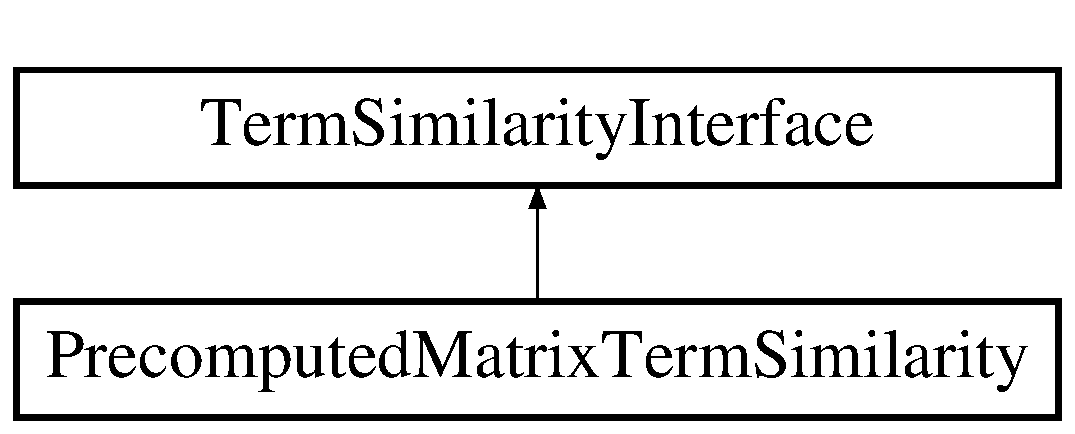
\includegraphics[height=2.000000cm]{classPrecomputedMatrixTermSimilarity}
\end{center}
\end{figure}
\subsection*{Public Member Functions}
\begin{DoxyCompactItemize}
\item 
\hyperlink{classPrecomputedMatrixTermSimilarity_a7b41f4870cea2125e2997fb5eea5f6fb}{Precomputed\+Matrix\+Term\+Similarity} (std\+::string matrix\+\_\+file)
\begin{DoxyCompactList}\small\item\em A constructor. \end{DoxyCompactList}\item 
double \hyperlink{classPrecomputedMatrixTermSimilarity_accf2925db5da35cc040f2016813ed631}{calculate\+Term\+Similarity} (std\+::string go\+TermA, std\+::string go\+TermB)
\begin{DoxyCompactList}\small\item\em A method for calculating term-\/to-\/term similarity for \hyperlink{namespaceGO}{GO} terms using a precomputed similarity matrix. \end{DoxyCompactList}\item 
double \hyperlink{classPrecomputedMatrixTermSimilarity_ac2057bd30526a99741c06f8b629b6ae2}{calculate\+Normalized\+Term\+Similarity} (std\+::string go\+TermA, std\+::string go\+TermB)
\begin{DoxyCompactList}\small\item\em A method for calculating term-\/to-\/term similarity for \hyperlink{namespaceGO}{GO} terms using a precomputed similarity matrix. \end{DoxyCompactList}\item 
std\+::vector$<$ double $>$ \hyperlink{classPrecomputedMatrixTermSimilarity_a341a4dba0540acd9087091aa63c51220}{project\+Term\+Set} (const std\+::vector$<$ std\+::string $>$ \&terms)
\begin{DoxyCompactList}\small\item\em This method projects a set of terms into it the kernel space. \end{DoxyCompactList}\end{DoxyCompactItemize}


\subsection{Detailed Description}
A class to calculate similarity between go terms for 2 sets using a precomuted term similarity matrix. 

This class allows the term similarity calculation to be decoupled from term set (gene) similarity measure that use them. Term similarity is loaded from a matrix file. 

\subsection{Constructor \& Destructor Documentation}
\index{Precomputed\+Matrix\+Term\+Similarity@{Precomputed\+Matrix\+Term\+Similarity}!Precomputed\+Matrix\+Term\+Similarity@{Precomputed\+Matrix\+Term\+Similarity}}
\index{Precomputed\+Matrix\+Term\+Similarity@{Precomputed\+Matrix\+Term\+Similarity}!Precomputed\+Matrix\+Term\+Similarity@{Precomputed\+Matrix\+Term\+Similarity}}
\subsubsection[{\texorpdfstring{Precomputed\+Matrix\+Term\+Similarity(std\+::string matrix\+\_\+file)}{PrecomputedMatrixTermSimilarity(std::string matrix_file)}}]{\setlength{\rightskip}{0pt plus 5cm}Precomputed\+Matrix\+Term\+Similarity\+::\+Precomputed\+Matrix\+Term\+Similarity (
\begin{DoxyParamCaption}
\item[{std\+::string}]{matrix\+\_\+file}
\end{DoxyParamCaption}
)\hspace{0.3cm}{\ttfamily [inline]}}\hypertarget{classPrecomputedMatrixTermSimilarity_a7b41f4870cea2125e2997fb5eea5f6fb}{}\label{classPrecomputedMatrixTermSimilarity_a7b41f4870cea2125e2997fb5eea5f6fb}


A constructor. 

Parses a matrix file and creates the \hyperlink{classPrecomputedMatrixTermSimilarity}{Precomputed\+Matrix\+Term\+Similarity} object 

\subsection{Member Function Documentation}
\index{Precomputed\+Matrix\+Term\+Similarity@{Precomputed\+Matrix\+Term\+Similarity}!calculate\+Normalized\+Term\+Similarity@{calculate\+Normalized\+Term\+Similarity}}
\index{calculate\+Normalized\+Term\+Similarity@{calculate\+Normalized\+Term\+Similarity}!Precomputed\+Matrix\+Term\+Similarity@{Precomputed\+Matrix\+Term\+Similarity}}
\subsubsection[{\texorpdfstring{calculate\+Normalized\+Term\+Similarity(std\+::string go\+Term\+A, std\+::string go\+Term\+B)}{calculateNormalizedTermSimilarity(std::string goTermA, std::string goTermB)}}]{\setlength{\rightskip}{0pt plus 5cm}double Precomputed\+Matrix\+Term\+Similarity\+::calculate\+Normalized\+Term\+Similarity (
\begin{DoxyParamCaption}
\item[{std\+::string}]{go\+TermA, }
\item[{std\+::string}]{go\+TermB}
\end{DoxyParamCaption}
)\hspace{0.3cm}{\ttfamily [inline]}, {\ttfamily [virtual]}}\hypertarget{classPrecomputedMatrixTermSimilarity_ac2057bd30526a99741c06f8b629b6ae2}{}\label{classPrecomputedMatrixTermSimilarity_ac2057bd30526a99741c06f8b629b6ae2}


A method for calculating term-\/to-\/term similarity for \hyperlink{namespaceGO}{GO} terms using a precomputed similarity matrix. 

This method returns the similarity scaled between 0 and 1 \mbox{[}0,1\mbox{]} inclusive 

Implements \hyperlink{classTermSimilarityInterface_aa46b7870c7725faab85ec502a3e5242d}{Term\+Similarity\+Interface}.

\index{Precomputed\+Matrix\+Term\+Similarity@{Precomputed\+Matrix\+Term\+Similarity}!calculate\+Term\+Similarity@{calculate\+Term\+Similarity}}
\index{calculate\+Term\+Similarity@{calculate\+Term\+Similarity}!Precomputed\+Matrix\+Term\+Similarity@{Precomputed\+Matrix\+Term\+Similarity}}
\subsubsection[{\texorpdfstring{calculate\+Term\+Similarity(std\+::string go\+Term\+A, std\+::string go\+Term\+B)}{calculateTermSimilarity(std::string goTermA, std::string goTermB)}}]{\setlength{\rightskip}{0pt plus 5cm}double Precomputed\+Matrix\+Term\+Similarity\+::calculate\+Term\+Similarity (
\begin{DoxyParamCaption}
\item[{std\+::string}]{go\+TermA, }
\item[{std\+::string}]{go\+TermB}
\end{DoxyParamCaption}
)\hspace{0.3cm}{\ttfamily [inline]}, {\ttfamily [virtual]}}\hypertarget{classPrecomputedMatrixTermSimilarity_accf2925db5da35cc040f2016813ed631}{}\label{classPrecomputedMatrixTermSimilarity_accf2925db5da35cc040f2016813ed631}


A method for calculating term-\/to-\/term similarity for \hyperlink{namespaceGO}{GO} terms using a precomputed similarity matrix. 

This method returns the term similarity as defined by the matrix. 

Implements \hyperlink{classTermSimilarityInterface_ae3474adcfcb02faef65ed5e16ef4db47}{Term\+Similarity\+Interface}.

\index{Precomputed\+Matrix\+Term\+Similarity@{Precomputed\+Matrix\+Term\+Similarity}!project\+Term\+Set@{project\+Term\+Set}}
\index{project\+Term\+Set@{project\+Term\+Set}!Precomputed\+Matrix\+Term\+Similarity@{Precomputed\+Matrix\+Term\+Similarity}}
\subsubsection[{\texorpdfstring{project\+Term\+Set(const std\+::vector$<$ std\+::string $>$ \&terms)}{projectTermSet(const std::vector< std::string > &terms)}}]{\setlength{\rightskip}{0pt plus 5cm}std\+::vector$<$double$>$ Precomputed\+Matrix\+Term\+Similarity\+::project\+Term\+Set (
\begin{DoxyParamCaption}
\item[{const std\+::vector$<$ std\+::string $>$ \&}]{terms}
\end{DoxyParamCaption}
)\hspace{0.3cm}{\ttfamily [inline]}}\hypertarget{classPrecomputedMatrixTermSimilarity_a341a4dba0540acd9087091aa63c51220}{}\label{classPrecomputedMatrixTermSimilarity_a341a4dba0540acd9087091aa63c51220}


This method projects a set of terms into it the kernel space. 

This method treats the term similarity matrix as a kernel and projects a set of terms into it. 

The documentation for this class was generated from the following file\+:\begin{DoxyCompactItemize}
\item 
ggtk/Precomputed\+Matrix\+Term\+Similarity.\+hpp\end{DoxyCompactItemize}

\hypertarget{classRapidXmlGoParser}{}\section{Rapid\+Xml\+Go\+Parser Class Reference}
\label{classRapidXmlGoParser}\index{Rapid\+Xml\+Go\+Parser@{Rapid\+Xml\+Go\+Parser}}


This class parses a go X\+ML file using Rapid\+X\+ML library.  




{\ttfamily \#include $<$ggtk/\+Rapid\+Xml\+Go\+Parser.\+hpp$>$}

Inheritance diagram for Rapid\+Xml\+Go\+Parser\+:\begin{figure}[H]
\begin{center}
\leavevmode
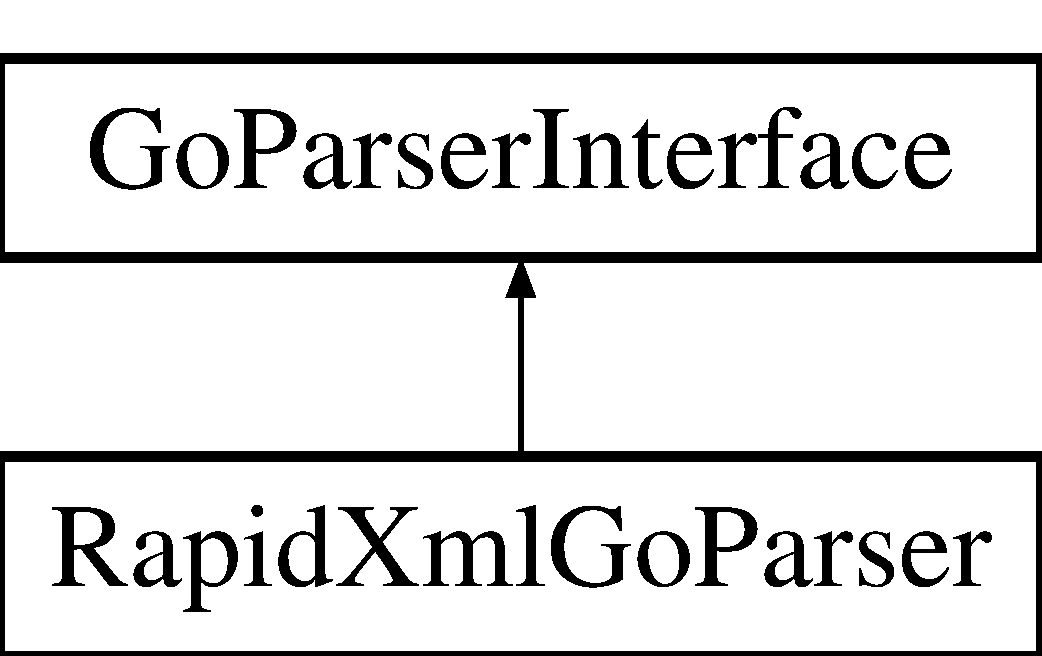
\includegraphics[height=2.000000cm]{classRapidXmlGoParser}
\end{center}
\end{figure}
\subsection*{Public Member Functions}
\begin{DoxyCompactItemize}
\item 
\hyperlink{classGoGraph}{Go\+Graph} $\ast$ \hyperlink{classRapidXmlGoParser_a7c42085d86c58983601fdada4aaacd9d}{parse\+Go\+File} (std\+::string filename)
\begin{DoxyCompactList}\small\item\em Method to parse the go file, should be an X\+ML file. \end{DoxyCompactList}\item 
bool \hyperlink{classRapidXmlGoParser_a945a31fd86bd35720d4158caa35302da}{is\+File\+Good} (const std\+::string \&filename)
\begin{DoxyCompactList}\small\item\em A method to test if a file fits the accepted format. \end{DoxyCompactList}\item 
\hyperlink{classGoParserInterface}{Go\+Parser\+Interface} $\ast$ \hyperlink{classRapidXmlGoParser_af69641207e01be186f523939ce03f847}{clone} ()
\begin{DoxyCompactList}\small\item\em A method to create a new instance of this class for use in a factory. \end{DoxyCompactList}\end{DoxyCompactItemize}


\subsection{Detailed Description}
This class parses a go X\+ML file using Rapid\+X\+ML library. 

This class parses a Gene Ontology X\+ML file using Rapid\+X\+ML library.

Implements \hyperlink{classGoParserInterface}{Go\+Parser\+Interface} 

\subsection{Member Function Documentation}
\index{Rapid\+Xml\+Go\+Parser@{Rapid\+Xml\+Go\+Parser}!clone@{clone}}
\index{clone@{clone}!Rapid\+Xml\+Go\+Parser@{Rapid\+Xml\+Go\+Parser}}
\subsubsection[{\texorpdfstring{clone()}{clone()}}]{\setlength{\rightskip}{0pt plus 5cm}{\bf Go\+Parser\+Interface}$\ast$ Rapid\+Xml\+Go\+Parser\+::clone (
\begin{DoxyParamCaption}
{}
\end{DoxyParamCaption}
)\hspace{0.3cm}{\ttfamily [inline]}, {\ttfamily [virtual]}}\hypertarget{classRapidXmlGoParser_af69641207e01be186f523939ce03f847}{}\label{classRapidXmlGoParser_af69641207e01be186f523939ce03f847}


A method to create a new instance of this class for use in a factory. 

creats a new pointer to the parser, used by the factory for go parsers. 

Implements \hyperlink{classGoParserInterface_a21c4ea01809737ab2975fb71edf6fcd5}{Go\+Parser\+Interface}.

\index{Rapid\+Xml\+Go\+Parser@{Rapid\+Xml\+Go\+Parser}!is\+File\+Good@{is\+File\+Good}}
\index{is\+File\+Good@{is\+File\+Good}!Rapid\+Xml\+Go\+Parser@{Rapid\+Xml\+Go\+Parser}}
\subsubsection[{\texorpdfstring{is\+File\+Good(const std\+::string \&filename)}{isFileGood(const std::string &filename)}}]{\setlength{\rightskip}{0pt plus 5cm}bool Rapid\+Xml\+Go\+Parser\+::is\+File\+Good (
\begin{DoxyParamCaption}
\item[{const std\+::string \&}]{filename}
\end{DoxyParamCaption}
)\hspace{0.3cm}{\ttfamily [inline]}, {\ttfamily [virtual]}}\hypertarget{classRapidXmlGoParser_a945a31fd86bd35720d4158caa35302da}{}\label{classRapidXmlGoParser_a945a31fd86bd35720d4158caa35302da}


A method to test if a file fits the accepted format. 

Returns true if the file matches accepted format, false otherwise 

Implements \hyperlink{classGoParserInterface_a0d2db54063c1ff58a0e15f0187af5aa1}{Go\+Parser\+Interface}.

\index{Rapid\+Xml\+Go\+Parser@{Rapid\+Xml\+Go\+Parser}!parse\+Go\+File@{parse\+Go\+File}}
\index{parse\+Go\+File@{parse\+Go\+File}!Rapid\+Xml\+Go\+Parser@{Rapid\+Xml\+Go\+Parser}}
\subsubsection[{\texorpdfstring{parse\+Go\+File(std\+::string filename)}{parseGoFile(std::string filename)}}]{\setlength{\rightskip}{0pt plus 5cm}{\bf Go\+Graph}$\ast$ Rapid\+Xml\+Go\+Parser\+::parse\+Go\+File (
\begin{DoxyParamCaption}
\item[{std\+::string}]{filename}
\end{DoxyParamCaption}
)\hspace{0.3cm}{\ttfamily [inline]}, {\ttfamily [virtual]}}\hypertarget{classRapidXmlGoParser_a7c42085d86c58983601fdada4aaacd9d}{}\label{classRapidXmlGoParser_a7c42085d86c58983601fdada4aaacd9d}


Method to parse the go file, should be an X\+ML file. 

This method will read a Gene Ontology X\+ML file and add all relationships to the graph. 

Implements \hyperlink{classGoParserInterface_aefde440e0d5404b9efa2a16a89e09674}{Go\+Parser\+Interface}.



The documentation for this class was generated from the following file\+:\begin{DoxyCompactItemize}
\item 
ggtk/Rapid\+Xml\+Go\+Parser.\+hpp\end{DoxyCompactItemize}

\hypertarget{classRelationshipPolicyInterface}{}\section{Relationship\+Policy\+Interface Class Reference}
\label{classRelationshipPolicyInterface}\index{Relationship\+Policy\+Interface@{Relationship\+Policy\+Interface}}


An interface to check relationships between \hyperlink{namespaceGO}{GO} terms.  




{\ttfamily \#include $<$ggtk/\+Relationship\+Policy\+Interface.\+hpp$>$}

Inheritance diagram for Relationship\+Policy\+Interface\+:\begin{figure}[H]
\begin{center}
\leavevmode
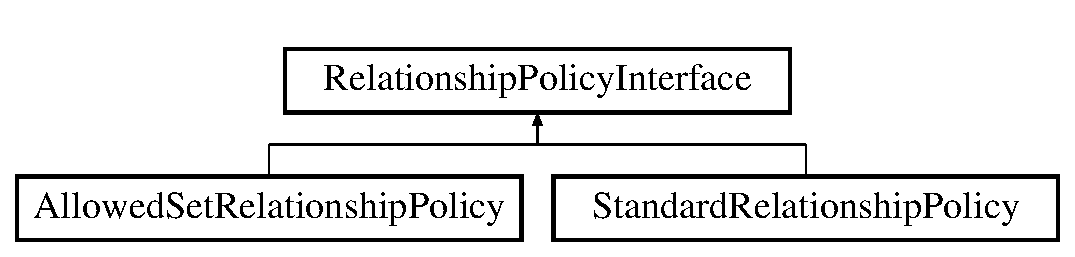
\includegraphics[height=2.000000cm]{classRelationshipPolicyInterface}
\end{center}
\end{figure}
\subsection*{Public Member Functions}
\begin{DoxyCompactItemize}
\item 
virtual bool \hyperlink{classRelationshipPolicyInterface_ad28012b607e9cf848c791b6a907bb2cb}{is\+Allowed} (\hyperlink{namespaceGO_aaa3905b2e000a8be411da8038827f993}{G\+O\+::\+Relationship} relationship)=0
\begin{DoxyCompactList}\small\item\em A pure virtual meethod to test if a relationship is allowed. \end{DoxyCompactList}\end{DoxyCompactItemize}


\subsection{Detailed Description}
An interface to check relationships between \hyperlink{namespaceGO}{GO} terms. 

This is interface is used to create parsers which will only use a specific set of relationship when parsing a \hyperlink{namespaceGO}{GO} graph file. 

\subsection{Member Function Documentation}
\index{Relationship\+Policy\+Interface@{Relationship\+Policy\+Interface}!is\+Allowed@{is\+Allowed}}
\index{is\+Allowed@{is\+Allowed}!Relationship\+Policy\+Interface@{Relationship\+Policy\+Interface}}
\subsubsection[{\texorpdfstring{is\+Allowed(\+G\+O\+::\+Relationship relationship)=0}{isAllowed(GO::Relationship relationship)=0}}]{\setlength{\rightskip}{0pt plus 5cm}virtual bool Relationship\+Policy\+Interface\+::is\+Allowed (
\begin{DoxyParamCaption}
\item[{{\bf G\+O\+::\+Relationship}}]{relationship}
\end{DoxyParamCaption}
)\hspace{0.3cm}{\ttfamily [pure virtual]}}\hypertarget{classRelationshipPolicyInterface_ad28012b607e9cf848c791b6a907bb2cb}{}\label{classRelationshipPolicyInterface_ad28012b607e9cf848c791b6a907bb2cb}


A pure virtual meethod to test if a relationship is allowed. 

This pure virtual method requires any subclass to imlement an is\+Allowed method to enforce the relationship pollicy. 

Implemented in \hyperlink{classAllowedSetRelationshipPolicy_ac7454bc649241219f076779330977f90}{Allowed\+Set\+Relationship\+Policy}, and \hyperlink{classStandardRelationshipPolicy_a75acddf7f5106cacf58f74bd837b03e4}{Standard\+Relationship\+Policy}.



The documentation for this class was generated from the following file\+:\begin{DoxyCompactItemize}
\item 
ggtk/Relationship\+Policy\+Interface.\+hpp\end{DoxyCompactItemize}

\hypertarget{classRelevanceSimilarity}{}\section{Relevance\+Similarity Class Reference}
\label{classRelevanceSimilarity}\index{Relevance\+Similarity@{Relevance\+Similarity}}


A class to calculate Relevance similarity between 2 terms.  




{\ttfamily \#include $<$ggtk/\+Relevance\+Similarity.\+hpp$>$}

Inheritance diagram for Relevance\+Similarity\+:\begin{figure}[H]
\begin{center}
\leavevmode
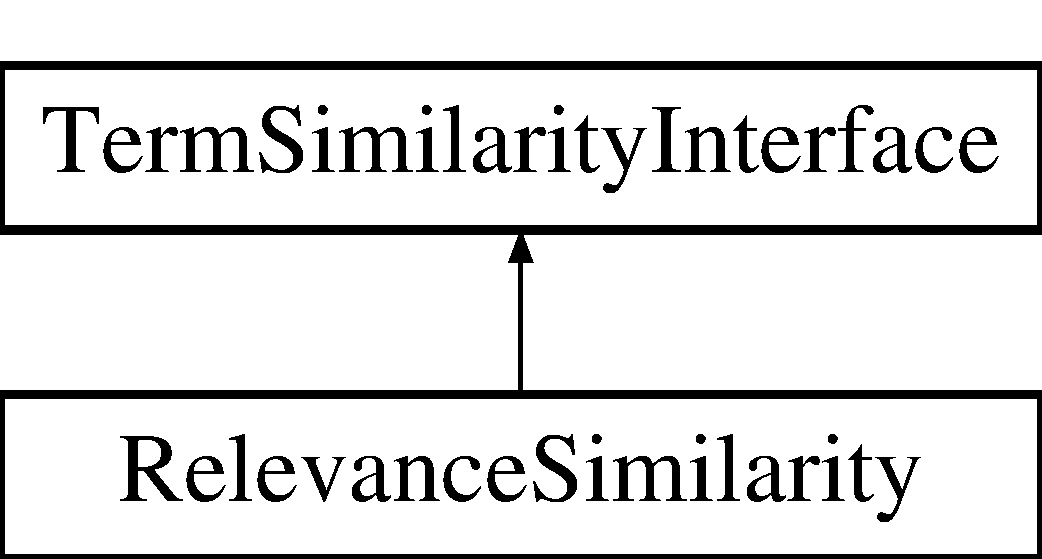
\includegraphics[height=2.000000cm]{classRelevanceSimilarity}
\end{center}
\end{figure}
\subsection*{Public Member Functions}
\begin{DoxyCompactItemize}
\item 
\hyperlink{classRelevanceSimilarity_a8c53e47a65cc1cb78aca2e94671b6534}{Relevance\+Similarity} (\hyperlink{classGoGraph}{Go\+Graph} $\ast$go\+Graph, \hyperlink{classTermInformationContentMap}{Term\+Information\+Content\+Map} \&ic\+Map)
\begin{DoxyCompactList}\small\item\em A constructor. \end{DoxyCompactList}\item 
double \hyperlink{classRelevanceSimilarity_a77fd7721c3c98611328f97b6b8c3f9e3}{calculate\+Term\+Similarity} (std\+::string go\+TermA, std\+::string go\+TermB)
\begin{DoxyCompactList}\small\item\em A method for calculating term-\/to-\/term similarity for \hyperlink{namespaceGO}{GO} terms using Relevance similarity. \end{DoxyCompactList}\item 
double \hyperlink{classRelevanceSimilarity_ad54bb47157112a225b353c47d1e2fad5}{calculate\+Normalized\+Term\+Similarity} (std\+::string go\+TermA, std\+::string go\+TermB)
\begin{DoxyCompactList}\small\item\em A method for calculating term-\/to-\/term similarity for \hyperlink{namespaceGO}{GO} terms using Normalized Relevance similarity. \end{DoxyCompactList}\item 
std\+::string \hyperlink{classRelevanceSimilarity_aa1db55c7a378e45ff66565e5e1043a8e}{get\+M\+I\+CA} (boost\+::unordered\+\_\+set$<$ std\+::string $>$ \&ancestorsA, boost\+::unordered\+\_\+set$<$ std\+::string $>$ \&ancestorsB)
\begin{DoxyCompactList}\small\item\em A method for calculating the most informative common ancestor. \end{DoxyCompactList}\end{DoxyCompactItemize}


\subsection{Detailed Description}
A class to calculate Relevance similarity between 2 terms. 

This class calculates Relevance similarity.

A. Schlicker, F. S. Domingues, J. Rahnenfuhrer, and T. Lengauer, \char`\"{}\+A new measure for functional similarity of gene products based
 on Gene Ontology,\char`\"{} B\+MC Bioinformatics, vol. 7, p. 302, 2006.

P. W. Lord, R. D. Stevens, A. Brass, and C. A. Goble, \char`\"{}\+Semantic similarity measures as tools for exploring the gene ontology,\char`\"{} Pac Symp Biocomput, pp. 601-\/12, 2003.

Basically this is Lin similarity scaled by the complement of the probability of the mica 2 $\ast$ I\+C(\+M\+I\+C\+A) / ( I\+C(term\+A) + I\+C(term\+B) )$\ast$(1-\/p(Mica)) 

\subsection{Constructor \& Destructor Documentation}
\index{Relevance\+Similarity@{Relevance\+Similarity}!Relevance\+Similarity@{Relevance\+Similarity}}
\index{Relevance\+Similarity@{Relevance\+Similarity}!Relevance\+Similarity@{Relevance\+Similarity}}
\subsubsection[{\texorpdfstring{Relevance\+Similarity(\+Go\+Graph $\ast$go\+Graph, Term\+Information\+Content\+Map \&ic\+Map)}{RelevanceSimilarity(GoGraph *goGraph, TermInformationContentMap &icMap)}}]{\setlength{\rightskip}{0pt plus 5cm}Relevance\+Similarity\+::\+Relevance\+Similarity (
\begin{DoxyParamCaption}
\item[{{\bf Go\+Graph} $\ast$}]{go\+Graph, }
\item[{{\bf Term\+Information\+Content\+Map} \&}]{ic\+Map}
\end{DoxyParamCaption}
)\hspace{0.3cm}{\ttfamily [inline]}}\hypertarget{classRelevanceSimilarity_a8c53e47a65cc1cb78aca2e94671b6534}{}\label{classRelevanceSimilarity_a8c53e47a65cc1cb78aca2e94671b6534}


A constructor. 

Creates the default(empty) \hyperlink{classStandardRelationshipPolicy}{Standard\+Relationship\+Policy} 

\subsection{Member Function Documentation}
\index{Relevance\+Similarity@{Relevance\+Similarity}!calculate\+Normalized\+Term\+Similarity@{calculate\+Normalized\+Term\+Similarity}}
\index{calculate\+Normalized\+Term\+Similarity@{calculate\+Normalized\+Term\+Similarity}!Relevance\+Similarity@{Relevance\+Similarity}}
\subsubsection[{\texorpdfstring{calculate\+Normalized\+Term\+Similarity(std\+::string go\+Term\+A, std\+::string go\+Term\+B)}{calculateNormalizedTermSimilarity(std::string goTermA, std::string goTermB)}}]{\setlength{\rightskip}{0pt plus 5cm}double Relevance\+Similarity\+::calculate\+Normalized\+Term\+Similarity (
\begin{DoxyParamCaption}
\item[{std\+::string}]{go\+TermA, }
\item[{std\+::string}]{go\+TermB}
\end{DoxyParamCaption}
)\hspace{0.3cm}{\ttfamily [inline]}, {\ttfamily [virtual]}}\hypertarget{classRelevanceSimilarity_ad54bb47157112a225b353c47d1e2fad5}{}\label{classRelevanceSimilarity_ad54bb47157112a225b353c47d1e2fad5}


A method for calculating term-\/to-\/term similarity for \hyperlink{namespaceGO}{GO} terms using Normalized Relevance similarity. 

This method returns the Relevance similarity scaled between 0 and 1 \mbox{[}0,1\mbox{]} inclusive 

Implements \hyperlink{classTermSimilarityInterface_aa46b7870c7725faab85ec502a3e5242d}{Term\+Similarity\+Interface}.

\index{Relevance\+Similarity@{Relevance\+Similarity}!calculate\+Term\+Similarity@{calculate\+Term\+Similarity}}
\index{calculate\+Term\+Similarity@{calculate\+Term\+Similarity}!Relevance\+Similarity@{Relevance\+Similarity}}
\subsubsection[{\texorpdfstring{calculate\+Term\+Similarity(std\+::string go\+Term\+A, std\+::string go\+Term\+B)}{calculateTermSimilarity(std::string goTermA, std::string goTermB)}}]{\setlength{\rightskip}{0pt plus 5cm}double Relevance\+Similarity\+::calculate\+Term\+Similarity (
\begin{DoxyParamCaption}
\item[{std\+::string}]{go\+TermA, }
\item[{std\+::string}]{go\+TermB}
\end{DoxyParamCaption}
)\hspace{0.3cm}{\ttfamily [inline]}, {\ttfamily [virtual]}}\hypertarget{classRelevanceSimilarity_a77fd7721c3c98611328f97b6b8c3f9e3}{}\label{classRelevanceSimilarity_a77fd7721c3c98611328f97b6b8c3f9e3}


A method for calculating term-\/to-\/term similarity for \hyperlink{namespaceGO}{GO} terms using Relevance similarity. 

This method returns the Relevance similarity. 

Implements \hyperlink{classTermSimilarityInterface_ae3474adcfcb02faef65ed5e16ef4db47}{Term\+Similarity\+Interface}.

\index{Relevance\+Similarity@{Relevance\+Similarity}!get\+M\+I\+CA@{get\+M\+I\+CA}}
\index{get\+M\+I\+CA@{get\+M\+I\+CA}!Relevance\+Similarity@{Relevance\+Similarity}}
\subsubsection[{\texorpdfstring{get\+M\+I\+C\+A(boost\+::unordered\+\_\+set$<$ std\+::string $>$ \&ancestors\+A, boost\+::unordered\+\_\+set$<$ std\+::string $>$ \&ancestors\+B)}{getMICA(boost::unordered_set< std::string > &ancestorsA, boost::unordered_set< std::string > &ancestorsB)}}]{\setlength{\rightskip}{0pt plus 5cm}std\+::string Relevance\+Similarity\+::get\+M\+I\+CA (
\begin{DoxyParamCaption}
\item[{boost\+::unordered\+\_\+set$<$ std\+::string $>$ \&}]{ancestorsA, }
\item[{boost\+::unordered\+\_\+set$<$ std\+::string $>$ \&}]{ancestorsB}
\end{DoxyParamCaption}
)\hspace{0.3cm}{\ttfamily [inline]}}\hypertarget{classRelevanceSimilarity_aa1db55c7a378e45ff66565e5e1043a8e}{}\label{classRelevanceSimilarity_aa1db55c7a378e45ff66565e5e1043a8e}


A method for calculating the most informative common ancestor. 

This method searches the sets to determine the most informatics ancestor. 

The documentation for this class was generated from the following file\+:\begin{DoxyCompactItemize}
\item 
ggtk/Relevance\+Similarity.\+hpp\end{DoxyCompactItemize}

\hypertarget{classResnikSimilarity}{}\section{Resnik\+Similarity Class Reference}
\label{classResnikSimilarity}\index{Resnik\+Similarity@{Resnik\+Similarity}}


A class to calculate resnik similarity between 2 terms.  




{\ttfamily \#include $<$ggtk/\+Resnik\+Similarity.\+hpp$>$}

Inheritance diagram for Resnik\+Similarity\+:\begin{figure}[H]
\begin{center}
\leavevmode
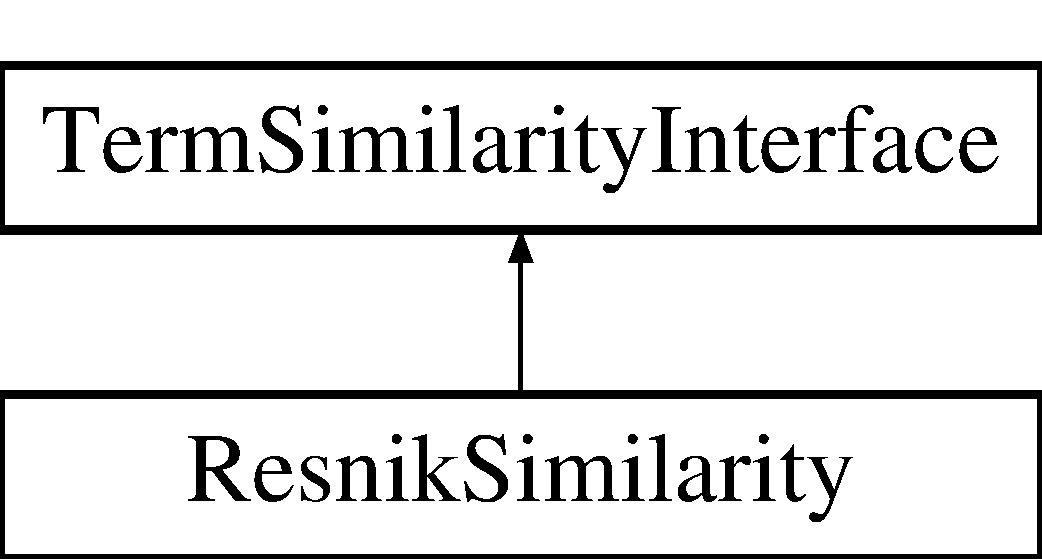
\includegraphics[height=2.000000cm]{classResnikSimilarity}
\end{center}
\end{figure}
\subsection*{Public Member Functions}
\begin{DoxyCompactItemize}
\item 
\hyperlink{classResnikSimilarity_a0e95354ebfc331dd4a73e823501378da}{Resnik\+Similarity} (\hyperlink{classGoGraph}{Go\+Graph} $\ast$go\+Graph, \hyperlink{classTermInformationContentMap}{Term\+Information\+Content\+Map} \&ic\+Map)
\begin{DoxyCompactList}\small\item\em A constructor. \end{DoxyCompactList}\item 
double \hyperlink{classResnikSimilarity_a340ace5dbdd105847d5fade4c8d20ade}{calculate\+Term\+Similarity} (std\+::string go\+TermA, std\+::string go\+TermB)
\begin{DoxyCompactList}\small\item\em A method for calculating term-\/to-\/term similarity for \hyperlink{namespaceGO}{GO} terms using Resnik similarity. \end{DoxyCompactList}\item 
double \hyperlink{classResnikSimilarity_a4e1d6ef4268a905a117fd0c054e4c39b}{calculate\+Normalized\+Term\+Similarity} (std\+::string go\+TermA, std\+::string go\+TermB)
\begin{DoxyCompactList}\small\item\em A method for calculating term-\/to-\/term similarity for \hyperlink{namespaceGO}{GO} terms using Normalized Resnik similarity. \end{DoxyCompactList}\item 
std\+::string \hyperlink{classResnikSimilarity_ace3ae20bcef468c53925e45c647584c0}{get\+M\+I\+CA} (boost\+::unordered\+\_\+set$<$ std\+::string $>$ \&ancestorsA, boost\+::unordered\+\_\+set$<$ std\+::string $>$ \&ancestorsB)
\begin{DoxyCompactList}\small\item\em A method for calculating the most informative common ancestor. \end{DoxyCompactList}\end{DoxyCompactItemize}


\subsection{Detailed Description}
A class to calculate resnik similarity between 2 terms. 

This class calculates Resnik similarity. Philip Resnik (1995). \char`\"{}\+Using information content to evaluate semantic similarity in a taxonomy\char`\"{}. In Chris S. Mellish (Ed.). Proceedings of the 14th international joint conference on Artificial intelligence (I\+J\+C\+AI\textquotesingle{}95)

P. W. Lord, R. D. Stevens, A. Brass, and C. A. Goble, \char`\"{}\+Semantic similarity measures as tools for exploring the gene ontology,\char`\"{} Pac Symp Biocomput, pp. 601-\/12, 2003.

maximun information content of all shared ancestors I\+C(\+M\+I\+C\+A) 

\subsection{Constructor \& Destructor Documentation}
\index{Resnik\+Similarity@{Resnik\+Similarity}!Resnik\+Similarity@{Resnik\+Similarity}}
\index{Resnik\+Similarity@{Resnik\+Similarity}!Resnik\+Similarity@{Resnik\+Similarity}}
\subsubsection[{\texorpdfstring{Resnik\+Similarity(\+Go\+Graph $\ast$go\+Graph, Term\+Information\+Content\+Map \&ic\+Map)}{ResnikSimilarity(GoGraph *goGraph, TermInformationContentMap &icMap)}}]{\setlength{\rightskip}{0pt plus 5cm}Resnik\+Similarity\+::\+Resnik\+Similarity (
\begin{DoxyParamCaption}
\item[{{\bf Go\+Graph} $\ast$}]{go\+Graph, }
\item[{{\bf Term\+Information\+Content\+Map} \&}]{ic\+Map}
\end{DoxyParamCaption}
)\hspace{0.3cm}{\ttfamily [inline]}}\hypertarget{classResnikSimilarity_a0e95354ebfc331dd4a73e823501378da}{}\label{classResnikSimilarity_a0e95354ebfc331dd4a73e823501378da}


A constructor. 

Creates the default(empty) \hyperlink{classStandardRelationshipPolicy}{Standard\+Relationship\+Policy} 

\subsection{Member Function Documentation}
\index{Resnik\+Similarity@{Resnik\+Similarity}!calculate\+Normalized\+Term\+Similarity@{calculate\+Normalized\+Term\+Similarity}}
\index{calculate\+Normalized\+Term\+Similarity@{calculate\+Normalized\+Term\+Similarity}!Resnik\+Similarity@{Resnik\+Similarity}}
\subsubsection[{\texorpdfstring{calculate\+Normalized\+Term\+Similarity(std\+::string go\+Term\+A, std\+::string go\+Term\+B)}{calculateNormalizedTermSimilarity(std::string goTermA, std::string goTermB)}}]{\setlength{\rightskip}{0pt plus 5cm}double Resnik\+Similarity\+::calculate\+Normalized\+Term\+Similarity (
\begin{DoxyParamCaption}
\item[{std\+::string}]{go\+TermA, }
\item[{std\+::string}]{go\+TermB}
\end{DoxyParamCaption}
)\hspace{0.3cm}{\ttfamily [inline]}, {\ttfamily [virtual]}}\hypertarget{classResnikSimilarity_a4e1d6ef4268a905a117fd0c054e4c39b}{}\label{classResnikSimilarity_a4e1d6ef4268a905a117fd0c054e4c39b}


A method for calculating term-\/to-\/term similarity for \hyperlink{namespaceGO}{GO} terms using Normalized Resnik similarity. 

This method returns the Resnik similarity divided by the maximum possible similarity 

Implements \hyperlink{classTermSimilarityInterface_aa46b7870c7725faab85ec502a3e5242d}{Term\+Similarity\+Interface}.

\index{Resnik\+Similarity@{Resnik\+Similarity}!calculate\+Term\+Similarity@{calculate\+Term\+Similarity}}
\index{calculate\+Term\+Similarity@{calculate\+Term\+Similarity}!Resnik\+Similarity@{Resnik\+Similarity}}
\subsubsection[{\texorpdfstring{calculate\+Term\+Similarity(std\+::string go\+Term\+A, std\+::string go\+Term\+B)}{calculateTermSimilarity(std::string goTermA, std::string goTermB)}}]{\setlength{\rightskip}{0pt plus 5cm}double Resnik\+Similarity\+::calculate\+Term\+Similarity (
\begin{DoxyParamCaption}
\item[{std\+::string}]{go\+TermA, }
\item[{std\+::string}]{go\+TermB}
\end{DoxyParamCaption}
)\hspace{0.3cm}{\ttfamily [inline]}, {\ttfamily [virtual]}}\hypertarget{classResnikSimilarity_a340ace5dbdd105847d5fade4c8d20ade}{}\label{classResnikSimilarity_a340ace5dbdd105847d5fade4c8d20ade}


A method for calculating term-\/to-\/term similarity for \hyperlink{namespaceGO}{GO} terms using Resnik similarity. 

This method returns the Resnik similarity or the information content of the most informative common ancestor. 

Implements \hyperlink{classTermSimilarityInterface_ae3474adcfcb02faef65ed5e16ef4db47}{Term\+Similarity\+Interface}.

\index{Resnik\+Similarity@{Resnik\+Similarity}!get\+M\+I\+CA@{get\+M\+I\+CA}}
\index{get\+M\+I\+CA@{get\+M\+I\+CA}!Resnik\+Similarity@{Resnik\+Similarity}}
\subsubsection[{\texorpdfstring{get\+M\+I\+C\+A(boost\+::unordered\+\_\+set$<$ std\+::string $>$ \&ancestors\+A, boost\+::unordered\+\_\+set$<$ std\+::string $>$ \&ancestors\+B)}{getMICA(boost::unordered_set< std::string > &ancestorsA, boost::unordered_set< std::string > &ancestorsB)}}]{\setlength{\rightskip}{0pt plus 5cm}std\+::string Resnik\+Similarity\+::get\+M\+I\+CA (
\begin{DoxyParamCaption}
\item[{boost\+::unordered\+\_\+set$<$ std\+::string $>$ \&}]{ancestorsA, }
\item[{boost\+::unordered\+\_\+set$<$ std\+::string $>$ \&}]{ancestorsB}
\end{DoxyParamCaption}
)\hspace{0.3cm}{\ttfamily [inline]}}\hypertarget{classResnikSimilarity_ace3ae20bcef468c53925e45c647584c0}{}\label{classResnikSimilarity_ace3ae20bcef468c53925e45c647584c0}


A method for calculating the most informative common ancestor. 

This method searches the sets to determine the most informatics ancestor. 

The documentation for this class was generated from the following file\+:\begin{DoxyCompactItemize}
\item 
ggtk/Resnik\+Similarity.\+hpp\end{DoxyCompactItemize}

\hypertarget{classSharedInformationInterface}{}\section{Shared\+Information\+Interface Class Reference}
\label{classSharedInformationInterface}\index{Shared\+Information\+Interface@{Shared\+Information\+Interface}}


An interface class to define shared information calculations.  




{\ttfamily \#include $<$ggtk/\+Shared\+Information\+Interface.\+hpp$>$}

Inheritance diagram for Shared\+Information\+Interface\+:\begin{figure}[H]
\begin{center}
\leavevmode
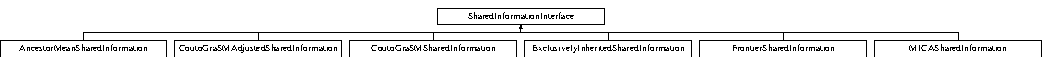
\includegraphics[height=0.761905cm]{classSharedInformationInterface}
\end{center}
\end{figure}
\subsection*{Public Member Functions}
\begin{DoxyCompactItemize}
\item 
virtual double \hyperlink{classSharedInformationInterface_a76e8858eb598442b86b0fd3be1c519e7}{shared\+Information} (const std\+::string \&termA, const std\+::string \&termB)=0
\begin{DoxyCompactList}\small\item\em A pure virtual method for returning the shared information of two terms. \end{DoxyCompactList}\item 
virtual double \hyperlink{classSharedInformationInterface_aba102c0e44fbc098baef6074f1eb37b6}{shared\+Information} (const std\+::string \&term)=0
\begin{DoxyCompactList}\small\item\em A pure virtual method for returning the shared information of a single terms,or information content. \end{DoxyCompactList}\item 
virtual double \hyperlink{classSharedInformationInterface_a7356ba99509458777972ce0f00ebd999}{max\+Information\+Content} (const std\+::string \&term)=0
\begin{DoxyCompactList}\small\item\em A pure virtual method for returning the maximum information content for a term. \end{DoxyCompactList}\item 
virtual bool \hyperlink{classSharedInformationInterface_a3f056cf6a40eea8c1669108087dcd5c8}{has\+Term} (const std\+::string \&term)=0
\begin{DoxyCompactList}\small\item\em A pure virtual method for determining if a term can be found. \end{DoxyCompactList}\item 
virtual bool \hyperlink{classSharedInformationInterface_a607463b9736df9c4b8ec3ba9fe41c19d}{is\+Same\+Ontology} (const std\+::string \&termA, const std\+::string \&termB)=0
\begin{DoxyCompactList}\small\item\em A pure virtual method for determining if the two terms are of like ontologies. \end{DoxyCompactList}\end{DoxyCompactItemize}


\subsection{Detailed Description}
An interface class to define shared information calculations. 

This class defines the interface for shared information calculations. Pure virtual methods require that shared information methods implement these. 

\subsection{Member Function Documentation}
\index{Shared\+Information\+Interface@{Shared\+Information\+Interface}!has\+Term@{has\+Term}}
\index{has\+Term@{has\+Term}!Shared\+Information\+Interface@{Shared\+Information\+Interface}}
\subsubsection[{\texorpdfstring{has\+Term(const std\+::string \&term)=0}{hasTerm(const std::string &term)=0}}]{\setlength{\rightskip}{0pt plus 5cm}virtual bool Shared\+Information\+Interface\+::has\+Term (
\begin{DoxyParamCaption}
\item[{const std\+::string \&}]{term}
\end{DoxyParamCaption}
)\hspace{0.3cm}{\ttfamily [pure virtual]}}\hypertarget{classSharedInformationInterface_a3f056cf6a40eea8c1669108087dcd5c8}{}\label{classSharedInformationInterface_a3f056cf6a40eea8c1669108087dcd5c8}


A pure virtual method for determining if a term can be found. 

This pure virtual method requires any shared information class to implement this method. This method provides a method for client classes to determine if a term can be found by the method. 

Implemented in \hyperlink{classCoutoGraSMSharedInformation_a718055d6fecea9e10125ae4895af7f95}{Couto\+Gra\+S\+M\+Shared\+Information}, \hyperlink{classCoutoGraSMAdjustedSharedInformation_ae6304b98a7c8784327f978ee59372ca3}{Couto\+Gra\+S\+M\+Adjusted\+Shared\+Information}, \hyperlink{classFrontierSharedInformation_a4cd9a78345443bdd8c43e7fcee01f9b4}{Frontier\+Shared\+Information}, \hyperlink{classExclusivelyInheritedSharedInformation_a0bf2231c6f714d97a5e55ee67893e403}{Exclusively\+Inherited\+Shared\+Information}, \hyperlink{classMICASharedInformation_a0fece18244af62c7e2258b0af418413a}{M\+I\+C\+A\+Shared\+Information}, and \hyperlink{classAncestorMeanSharedInformation_af7503d6f761957bcb22d0e6614d87fa4}{Ancestor\+Mean\+Shared\+Information}.

\index{Shared\+Information\+Interface@{Shared\+Information\+Interface}!is\+Same\+Ontology@{is\+Same\+Ontology}}
\index{is\+Same\+Ontology@{is\+Same\+Ontology}!Shared\+Information\+Interface@{Shared\+Information\+Interface}}
\subsubsection[{\texorpdfstring{is\+Same\+Ontology(const std\+::string \&term\+A, const std\+::string \&term\+B)=0}{isSameOntology(const std::string &termA, const std::string &termB)=0}}]{\setlength{\rightskip}{0pt plus 5cm}virtual bool Shared\+Information\+Interface\+::is\+Same\+Ontology (
\begin{DoxyParamCaption}
\item[{const std\+::string \&}]{termA, }
\item[{const std\+::string \&}]{termB}
\end{DoxyParamCaption}
)\hspace{0.3cm}{\ttfamily [pure virtual]}}\hypertarget{classSharedInformationInterface_a607463b9736df9c4b8ec3ba9fe41c19d}{}\label{classSharedInformationInterface_a607463b9736df9c4b8ec3ba9fe41c19d}


A pure virtual method for determining if the two terms are of like ontologies. 

This pure virtual method requires any shared information class to implement this method. This method provides a method for client classes to determine if two terms are of the same ontology. 

Implemented in \hyperlink{classCoutoGraSMSharedInformation_ae6e12a30f03b0c2232d73277d8d47cd1}{Couto\+Gra\+S\+M\+Shared\+Information}, \hyperlink{classCoutoGraSMAdjustedSharedInformation_a9e6387f431eddaf42a1b18529cb3a8f5}{Couto\+Gra\+S\+M\+Adjusted\+Shared\+Information}, \hyperlink{classFrontierSharedInformation_a545b12efcab4551d031fb6125f615080}{Frontier\+Shared\+Information}, \hyperlink{classExclusivelyInheritedSharedInformation_a7b0ec1a7a1fb653450686c7e31346363}{Exclusively\+Inherited\+Shared\+Information}, \hyperlink{classMICASharedInformation_a9cea24c8af57f17248ffe1f12fea9545}{M\+I\+C\+A\+Shared\+Information}, and \hyperlink{classAncestorMeanSharedInformation_a75f59ac9d53014b967d0a81de8a07dbb}{Ancestor\+Mean\+Shared\+Information}.

\index{Shared\+Information\+Interface@{Shared\+Information\+Interface}!max\+Information\+Content@{max\+Information\+Content}}
\index{max\+Information\+Content@{max\+Information\+Content}!Shared\+Information\+Interface@{Shared\+Information\+Interface}}
\subsubsection[{\texorpdfstring{max\+Information\+Content(const std\+::string \&term)=0}{maxInformationContent(const std::string &term)=0}}]{\setlength{\rightskip}{0pt plus 5cm}virtual double Shared\+Information\+Interface\+::max\+Information\+Content (
\begin{DoxyParamCaption}
\item[{const std\+::string \&}]{term}
\end{DoxyParamCaption}
)\hspace{0.3cm}{\ttfamily [pure virtual]}}\hypertarget{classSharedInformationInterface_a7356ba99509458777972ce0f00ebd999}{}\label{classSharedInformationInterface_a7356ba99509458777972ce0f00ebd999}


A pure virtual method for returning the maximum information content for a term. 

This pure virtual method requires any shared information class to implement this method. This method provides the absolute max information content with in a corpus for normalization purposes. 

Implemented in \hyperlink{classCoutoGraSMSharedInformation_ae97d2b59ecd6d1eeee2583c6005c65a2}{Couto\+Gra\+S\+M\+Shared\+Information}, \hyperlink{classCoutoGraSMAdjustedSharedInformation_ab66e18a4f169878ad2a9e9d6d3feb459}{Couto\+Gra\+S\+M\+Adjusted\+Shared\+Information}, \hyperlink{classFrontierSharedInformation_a8301888fc7343848a9ee307849e49125}{Frontier\+Shared\+Information}, \hyperlink{classExclusivelyInheritedSharedInformation_af435c2641f3ab4a34db2d473216ceb16}{Exclusively\+Inherited\+Shared\+Information}, \hyperlink{classMICASharedInformation_ae88d4a76721e03bbb418eb870fa18ff1}{M\+I\+C\+A\+Shared\+Information}, and \hyperlink{classAncestorMeanSharedInformation_abf7d613e1459a5cf49071871e55f8a50}{Ancestor\+Mean\+Shared\+Information}.

\index{Shared\+Information\+Interface@{Shared\+Information\+Interface}!shared\+Information@{shared\+Information}}
\index{shared\+Information@{shared\+Information}!Shared\+Information\+Interface@{Shared\+Information\+Interface}}
\subsubsection[{\texorpdfstring{shared\+Information(const std\+::string \&term\+A, const std\+::string \&term\+B)=0}{sharedInformation(const std::string &termA, const std::string &termB)=0}}]{\setlength{\rightskip}{0pt plus 5cm}virtual double Shared\+Information\+Interface\+::shared\+Information (
\begin{DoxyParamCaption}
\item[{const std\+::string \&}]{termA, }
\item[{const std\+::string \&}]{termB}
\end{DoxyParamCaption}
)\hspace{0.3cm}{\ttfamily [pure virtual]}}\hypertarget{classSharedInformationInterface_a76e8858eb598442b86b0fd3be1c519e7}{}\label{classSharedInformationInterface_a76e8858eb598442b86b0fd3be1c519e7}


A pure virtual method for returning the shared information of two terms. 

This pure virtual method requires any shared information class to implement this method. 

Implemented in \hyperlink{classCoutoGraSMSharedInformation_aeb3ea4684e5f198464ce9354171981d3}{Couto\+Gra\+S\+M\+Shared\+Information}, \hyperlink{classCoutoGraSMAdjustedSharedInformation_ac93a66e1b8efafc8cd1c166424241af9}{Couto\+Gra\+S\+M\+Adjusted\+Shared\+Information}, \hyperlink{classFrontierSharedInformation_afd0bf3ea7bb9f4f05f89cc2597bc2dcf}{Frontier\+Shared\+Information}, \hyperlink{classExclusivelyInheritedSharedInformation_ae7e51e7f1328cfc5f7b9991c7714eadf}{Exclusively\+Inherited\+Shared\+Information}, \hyperlink{classMICASharedInformation_a8f6329c173f2cd17caf1a65043e8e249}{M\+I\+C\+A\+Shared\+Information}, and \hyperlink{classAncestorMeanSharedInformation_a86dad7b02ff45ae758a2b311ad763350}{Ancestor\+Mean\+Shared\+Information}.

\index{Shared\+Information\+Interface@{Shared\+Information\+Interface}!shared\+Information@{shared\+Information}}
\index{shared\+Information@{shared\+Information}!Shared\+Information\+Interface@{Shared\+Information\+Interface}}
\subsubsection[{\texorpdfstring{shared\+Information(const std\+::string \&term)=0}{sharedInformation(const std::string &term)=0}}]{\setlength{\rightskip}{0pt plus 5cm}virtual double Shared\+Information\+Interface\+::shared\+Information (
\begin{DoxyParamCaption}
\item[{const std\+::string \&}]{term}
\end{DoxyParamCaption}
)\hspace{0.3cm}{\ttfamily [pure virtual]}}\hypertarget{classSharedInformationInterface_aba102c0e44fbc098baef6074f1eb37b6}{}\label{classSharedInformationInterface_aba102c0e44fbc098baef6074f1eb37b6}


A pure virtual method for returning the shared information of a single terms,or information content. 

This pure virtual method privdes a mechanism for returing a term\textquotesingle{}s infromation content. 

Implemented in \hyperlink{classCoutoGraSMSharedInformation_a1c9a0a709b77822cd3bc967beed08b66}{Couto\+Gra\+S\+M\+Shared\+Information}, \hyperlink{classCoutoGraSMAdjustedSharedInformation_a6a228833a96e710c4e143cefaf364a37}{Couto\+Gra\+S\+M\+Adjusted\+Shared\+Information}, \hyperlink{classFrontierSharedInformation_a7d9c15e312667dc5ac2af1c7e36f735b}{Frontier\+Shared\+Information}, \hyperlink{classExclusivelyInheritedSharedInformation_ad77022f2d6225c423fa0c5abb8a1443a}{Exclusively\+Inherited\+Shared\+Information}, \hyperlink{classMICASharedInformation_a230adc046f7f4bbab190aaef25d15a37}{M\+I\+C\+A\+Shared\+Information}, and \hyperlink{classAncestorMeanSharedInformation_af31937c58ee53db666586b446bc23061}{Ancestor\+Mean\+Shared\+Information}.



The documentation for this class was generated from the following file\+:\begin{DoxyCompactItemize}
\item 
ggtk/Shared\+Information\+Interface.\+hpp\end{DoxyCompactItemize}

\hypertarget{classSimpleRegion}{}\section{Simple\+Region Class Reference}
\label{classSimpleRegion}\index{Simple\+Region@{Simple\+Region}}


{\ttfamily \#include $<$ggtk/\+Simple\+Region.\+hpp$>$}

Inheritance diagram for Simple\+Region\+:\begin{figure}[H]
\begin{center}
\leavevmode
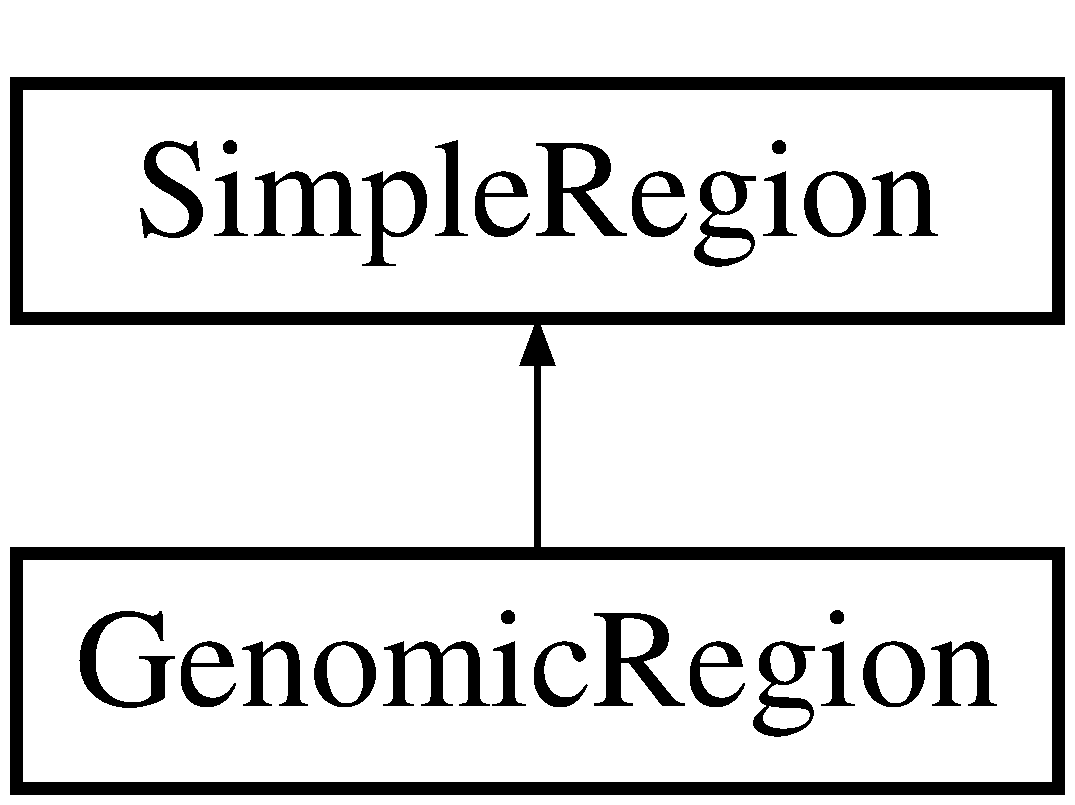
\includegraphics[height=2.000000cm]{classSimpleRegion}
\end{center}
\end{figure}
\subsection*{Public Member Functions}
\begin{DoxyCompactItemize}
\item 
\hyperlink{classSimpleRegion_a3f3502f62398e26fb88ea7b90ff7d3b8}{Simple\+Region} ()
\item 
\hyperlink{classSimpleRegion_a5432bba56f93741e76de989ccde3ecd5}{Simple\+Region} (const size\+\_\+t id, const size\+\_\+t start, const size\+\_\+t end)
\item 
const size\+\_\+t \hyperlink{classSimpleRegion_a3175b332ee5cbe1d6c83986666c481d0}{midpoint} () const 
\item 
int \hyperlink{classSimpleRegion_ab3e6068e293f2b8f0da920d8feb1f12b}{distance} (const \hyperlink{classSimpleRegion}{Simple\+Region} \&rhs)
\item 
bool \hyperlink{classSimpleRegion_aa0f04be989b3fd8726b60ea8af05408e}{contains} (const \hyperlink{classSimpleRegion}{Simple\+Region} \&rhs)
\item 
bool \hyperlink{classSimpleRegion_a71f1e66b268298559e319a39125b20e1}{contains} (const std\+::pair$<$ size\+\_\+t, size\+\_\+t $>$ \&rhs)
\item 
bool \hyperlink{classSimpleRegion_aedbd4cac0fc5318e612af3db76f19541}{contains} (const size\+\_\+t rhs\+\_\+start, const size\+\_\+t rhs\+\_\+end)
\item 
bool \hyperlink{classSimpleRegion_a39b10cf9d7ba8073da42e2cb95072bff}{contains} (const size\+\_\+t point)
\item 
bool \hyperlink{classSimpleRegion_a1f98da632e768077c967d63819cefedd}{overlaps} (const \hyperlink{classSimpleRegion}{Simple\+Region} \&rhs)
\item 
bool \hyperlink{classSimpleRegion_a0caf8d9707b7b0b29555e8bafd32ed47}{overlaps} (const std\+::pair$<$ size\+\_\+t, size\+\_\+t $>$ \&rhs)
\item 
bool \hyperlink{classSimpleRegion_a087f24f509cc26164a99e8509b720b28}{overlaps} (const size\+\_\+t rhs\+\_\+start, const size\+\_\+t rhs\+\_\+end)
\item 
size\+\_\+t \hyperlink{classSimpleRegion_a7c0d4f68409075dba1de716a328e9079}{get\+Start} ()
\item 
size\+\_\+t \hyperlink{classSimpleRegion_afb4924be3627dedec850a3ada174b083}{get\+End} ()
\item 
size\+\_\+t \hyperlink{classSimpleRegion_a1014d259fc8c94088b866be2d57835bc}{get\+Id} ()
\end{DoxyCompactItemize}
\subsection*{Public Attributes}
\begin{DoxyCompactItemize}
\item 
size\+\_\+t \hyperlink{classSimpleRegion_a397f3c8897d30259081e41ef9346745b}{\+\_\+id}
\item 
size\+\_\+t \hyperlink{classSimpleRegion_a24ee6f4ef0fc3ba2bfe9bc9eb8dfca60}{\+\_\+start}
\item 
size\+\_\+t \hyperlink{classSimpleRegion_aaf09baf8cd5cce7f8ad7083fd0b47e78}{\+\_\+end}
\end{DoxyCompactItemize}


\subsection{Detailed Description}
A Region class to be used with \hyperlink{classNCList}{N\+C\+List} This class is used to represent region and genome data. 

\subsection{Constructor \& Destructor Documentation}
\index{Simple\+Region@{Simple\+Region}!Simple\+Region@{Simple\+Region}}
\index{Simple\+Region@{Simple\+Region}!Simple\+Region@{Simple\+Region}}
\subsubsection[{\texorpdfstring{Simple\+Region()}{SimpleRegion()}}]{\setlength{\rightskip}{0pt plus 5cm}Simple\+Region\+::\+Simple\+Region (
\begin{DoxyParamCaption}
{}
\end{DoxyParamCaption}
)\hspace{0.3cm}{\ttfamily [inline]}}\hypertarget{classSimpleRegion_a3f3502f62398e26fb88ea7b90ff7d3b8}{}\label{classSimpleRegion_a3f3502f62398e26fb88ea7b90ff7d3b8}
Default constructor Initializes a simple region. \index{Simple\+Region@{Simple\+Region}!Simple\+Region@{Simple\+Region}}
\index{Simple\+Region@{Simple\+Region}!Simple\+Region@{Simple\+Region}}
\subsubsection[{\texorpdfstring{Simple\+Region(const size\+\_\+t id, const size\+\_\+t start, const size\+\_\+t end)}{SimpleRegion(const size_t id, const size_t start, const size_t end)}}]{\setlength{\rightskip}{0pt plus 5cm}Simple\+Region\+::\+Simple\+Region (
\begin{DoxyParamCaption}
\item[{const size\+\_\+t}]{id, }
\item[{const size\+\_\+t}]{start, }
\item[{const size\+\_\+t}]{end}
\end{DoxyParamCaption}
)\hspace{0.3cm}{\ttfamily [inline]}}\hypertarget{classSimpleRegion_a5432bba56f93741e76de989ccde3ecd5}{}\label{classSimpleRegion_a5432bba56f93741e76de989ccde3ecd5}
Parameterized constructor Allows the creation of a regions with user specified values 

\subsection{Member Function Documentation}
\index{Simple\+Region@{Simple\+Region}!contains@{contains}}
\index{contains@{contains}!Simple\+Region@{Simple\+Region}}
\subsubsection[{\texorpdfstring{contains(const Simple\+Region \&rhs)}{contains(const SimpleRegion &rhs)}}]{\setlength{\rightskip}{0pt plus 5cm}bool Simple\+Region\+::contains (
\begin{DoxyParamCaption}
\item[{const {\bf Simple\+Region} \&}]{rhs}
\end{DoxyParamCaption}
)\hspace{0.3cm}{\ttfamily [inline]}}\hypertarget{classSimpleRegion_aa0f04be989b3fd8726b60ea8af05408e}{}\label{classSimpleRegion_aa0f04be989b3fd8726b60ea8af05408e}
contains test with \hyperlink{classSimpleRegion}{Simple\+Region} objects. Does the region contain rhs? \index{Simple\+Region@{Simple\+Region}!contains@{contains}}
\index{contains@{contains}!Simple\+Region@{Simple\+Region}}
\subsubsection[{\texorpdfstring{contains(const std\+::pair$<$ size\+\_\+t, size\+\_\+t $>$ \&rhs)}{contains(const std::pair< size_t, size_t > &rhs)}}]{\setlength{\rightskip}{0pt plus 5cm}bool Simple\+Region\+::contains (
\begin{DoxyParamCaption}
\item[{const std\+::pair$<$ size\+\_\+t, size\+\_\+t $>$ \&}]{rhs}
\end{DoxyParamCaption}
)\hspace{0.3cm}{\ttfamily [inline]}}\hypertarget{classSimpleRegion_a71f1e66b268298559e319a39125b20e1}{}\label{classSimpleRegion_a71f1e66b268298559e319a39125b20e1}
Tests the contains relationship with a start end pair Does the region contain the start end pair? \index{Simple\+Region@{Simple\+Region}!contains@{contains}}
\index{contains@{contains}!Simple\+Region@{Simple\+Region}}
\subsubsection[{\texorpdfstring{contains(const size\+\_\+t rhs\+\_\+start, const size\+\_\+t rhs\+\_\+end)}{contains(const size_t rhs_start, const size_t rhs_end)}}]{\setlength{\rightskip}{0pt plus 5cm}bool Simple\+Region\+::contains (
\begin{DoxyParamCaption}
\item[{const size\+\_\+t}]{rhs\+\_\+start, }
\item[{const size\+\_\+t}]{rhs\+\_\+end}
\end{DoxyParamCaption}
)\hspace{0.3cm}{\ttfamily [inline]}}\hypertarget{classSimpleRegion_aedbd4cac0fc5318e612af3db76f19541}{}\label{classSimpleRegion_aedbd4cac0fc5318e612af3db76f19541}
Tests the contains relationship with start and end coordinates Does the region contain the interval between start and end? \index{Simple\+Region@{Simple\+Region}!contains@{contains}}
\index{contains@{contains}!Simple\+Region@{Simple\+Region}}
\subsubsection[{\texorpdfstring{contains(const size\+\_\+t point)}{contains(const size_t point)}}]{\setlength{\rightskip}{0pt plus 5cm}bool Simple\+Region\+::contains (
\begin{DoxyParamCaption}
\item[{const size\+\_\+t}]{point}
\end{DoxyParamCaption}
)\hspace{0.3cm}{\ttfamily [inline]}}\hypertarget{classSimpleRegion_a39b10cf9d7ba8073da42e2cb95072bff}{}\label{classSimpleRegion_a39b10cf9d7ba8073da42e2cb95072bff}
Tests the contains relationship with a single point Does the region contain the point coordinate? \index{Simple\+Region@{Simple\+Region}!distance@{distance}}
\index{distance@{distance}!Simple\+Region@{Simple\+Region}}
\subsubsection[{\texorpdfstring{distance(const Simple\+Region \&rhs)}{distance(const SimpleRegion &rhs)}}]{\setlength{\rightskip}{0pt plus 5cm}int Simple\+Region\+::distance (
\begin{DoxyParamCaption}
\item[{const {\bf Simple\+Region} \&}]{rhs}
\end{DoxyParamCaption}
)\hspace{0.3cm}{\ttfamily [inline]}}\hypertarget{classSimpleRegion_ab3e6068e293f2b8f0da920d8feb1f12b}{}\label{classSimpleRegion_ab3e6068e293f2b8f0da920d8feb1f12b}
Simple distance between two regions. Calculates the distance between two regions by calculating the distance between their midpoints. \index{Simple\+Region@{Simple\+Region}!get\+End@{get\+End}}
\index{get\+End@{get\+End}!Simple\+Region@{Simple\+Region}}
\subsubsection[{\texorpdfstring{get\+End()}{getEnd()}}]{\setlength{\rightskip}{0pt plus 5cm}size\+\_\+t Simple\+Region\+::get\+End (
\begin{DoxyParamCaption}
{}
\end{DoxyParamCaption}
)\hspace{0.3cm}{\ttfamily [inline]}}\hypertarget{classSimpleRegion_afb4924be3627dedec850a3ada174b083}{}\label{classSimpleRegion_afb4924be3627dedec850a3ada174b083}
accessor for end coordinate returns the interval\textquotesingle{}s end coordinate \index{Simple\+Region@{Simple\+Region}!get\+Id@{get\+Id}}
\index{get\+Id@{get\+Id}!Simple\+Region@{Simple\+Region}}
\subsubsection[{\texorpdfstring{get\+Id()}{getId()}}]{\setlength{\rightskip}{0pt plus 5cm}size\+\_\+t Simple\+Region\+::get\+Id (
\begin{DoxyParamCaption}
{}
\end{DoxyParamCaption}
)\hspace{0.3cm}{\ttfamily [inline]}}\hypertarget{classSimpleRegion_a1014d259fc8c94088b866be2d57835bc}{}\label{classSimpleRegion_a1014d259fc8c94088b866be2d57835bc}
accessor for the id returns the interval\textquotesingle{}s id \index{Simple\+Region@{Simple\+Region}!get\+Start@{get\+Start}}
\index{get\+Start@{get\+Start}!Simple\+Region@{Simple\+Region}}
\subsubsection[{\texorpdfstring{get\+Start()}{getStart()}}]{\setlength{\rightskip}{0pt plus 5cm}size\+\_\+t Simple\+Region\+::get\+Start (
\begin{DoxyParamCaption}
{}
\end{DoxyParamCaption}
)\hspace{0.3cm}{\ttfamily [inline]}}\hypertarget{classSimpleRegion_a7c0d4f68409075dba1de716a328e9079}{}\label{classSimpleRegion_a7c0d4f68409075dba1de716a328e9079}
accessor for start coordinate returns the interval\textquotesingle{}s start coordinate \index{Simple\+Region@{Simple\+Region}!midpoint@{midpoint}}
\index{midpoint@{midpoint}!Simple\+Region@{Simple\+Region}}
\subsubsection[{\texorpdfstring{midpoint() const }{midpoint() const }}]{\setlength{\rightskip}{0pt plus 5cm}const size\+\_\+t Simple\+Region\+::midpoint (
\begin{DoxyParamCaption}
{}
\end{DoxyParamCaption}
) const\hspace{0.3cm}{\ttfamily [inline]}}\hypertarget{classSimpleRegion_a3175b332ee5cbe1d6c83986666c481d0}{}\label{classSimpleRegion_a3175b332ee5cbe1d6c83986666c481d0}
Calculates the midpoint of a region Simple mid point of a region. (end -\/ start)/2 \index{Simple\+Region@{Simple\+Region}!overlaps@{overlaps}}
\index{overlaps@{overlaps}!Simple\+Region@{Simple\+Region}}
\subsubsection[{\texorpdfstring{overlaps(const Simple\+Region \&rhs)}{overlaps(const SimpleRegion &rhs)}}]{\setlength{\rightskip}{0pt plus 5cm}bool Simple\+Region\+::overlaps (
\begin{DoxyParamCaption}
\item[{const {\bf Simple\+Region} \&}]{rhs}
\end{DoxyParamCaption}
)\hspace{0.3cm}{\ttfamily [inline]}}\hypertarget{classSimpleRegion_a1f98da632e768077c967d63819cefedd}{}\label{classSimpleRegion_a1f98da632e768077c967d63819cefedd}
Tests the overlap relationship with a region Does the region overlap the rhs region? \index{Simple\+Region@{Simple\+Region}!overlaps@{overlaps}}
\index{overlaps@{overlaps}!Simple\+Region@{Simple\+Region}}
\subsubsection[{\texorpdfstring{overlaps(const std\+::pair$<$ size\+\_\+t, size\+\_\+t $>$ \&rhs)}{overlaps(const std::pair< size_t, size_t > &rhs)}}]{\setlength{\rightskip}{0pt plus 5cm}bool Simple\+Region\+::overlaps (
\begin{DoxyParamCaption}
\item[{const std\+::pair$<$ size\+\_\+t, size\+\_\+t $>$ \&}]{rhs}
\end{DoxyParamCaption}
)\hspace{0.3cm}{\ttfamily [inline]}}\hypertarget{classSimpleRegion_a0caf8d9707b7b0b29555e8bafd32ed47}{}\label{classSimpleRegion_a0caf8d9707b7b0b29555e8bafd32ed47}
Tests the overlap relationship with a start end pair Does the region overlap the start end pair? \index{Simple\+Region@{Simple\+Region}!overlaps@{overlaps}}
\index{overlaps@{overlaps}!Simple\+Region@{Simple\+Region}}
\subsubsection[{\texorpdfstring{overlaps(const size\+\_\+t rhs\+\_\+start, const size\+\_\+t rhs\+\_\+end)}{overlaps(const size_t rhs_start, const size_t rhs_end)}}]{\setlength{\rightskip}{0pt plus 5cm}bool Simple\+Region\+::overlaps (
\begin{DoxyParamCaption}
\item[{const size\+\_\+t}]{rhs\+\_\+start, }
\item[{const size\+\_\+t}]{rhs\+\_\+end}
\end{DoxyParamCaption}
)\hspace{0.3cm}{\ttfamily [inline]}}\hypertarget{classSimpleRegion_a087f24f509cc26164a99e8509b720b28}{}\label{classSimpleRegion_a087f24f509cc26164a99e8509b720b28}
Tests the overlap relationship with start and end coordinates Does the region overlap the interval defines by start and end? 

\subsection{Member Data Documentation}
\index{Simple\+Region@{Simple\+Region}!\+\_\+end@{\+\_\+end}}
\index{\+\_\+end@{\+\_\+end}!Simple\+Region@{Simple\+Region}}
\subsubsection[{\texorpdfstring{\+\_\+end}{_end}}]{\setlength{\rightskip}{0pt plus 5cm}size\+\_\+t Simple\+Region\+::\+\_\+end}\hypertarget{classSimpleRegion_aaf09baf8cd5cce7f8ad7083fd0b47e78}{}\label{classSimpleRegion_aaf09baf8cd5cce7f8ad7083fd0b47e78}
the end coordinate for the region \index{Simple\+Region@{Simple\+Region}!\+\_\+id@{\+\_\+id}}
\index{\+\_\+id@{\+\_\+id}!Simple\+Region@{Simple\+Region}}
\subsubsection[{\texorpdfstring{\+\_\+id}{_id}}]{\setlength{\rightskip}{0pt plus 5cm}size\+\_\+t Simple\+Region\+::\+\_\+id}\hypertarget{classSimpleRegion_a397f3c8897d30259081e41ef9346745b}{}\label{classSimpleRegion_a397f3c8897d30259081e41ef9346745b}
a generic id for the region \index{Simple\+Region@{Simple\+Region}!\+\_\+start@{\+\_\+start}}
\index{\+\_\+start@{\+\_\+start}!Simple\+Region@{Simple\+Region}}
\subsubsection[{\texorpdfstring{\+\_\+start}{_start}}]{\setlength{\rightskip}{0pt plus 5cm}size\+\_\+t Simple\+Region\+::\+\_\+start}\hypertarget{classSimpleRegion_a24ee6f4ef0fc3ba2bfe9bc9eb8dfca60}{}\label{classSimpleRegion_a24ee6f4ef0fc3ba2bfe9bc9eb8dfca60}
the start coordinate for the region 

The documentation for this class was generated from the following file\+:\begin{DoxyCompactItemize}
\item 
ggtk/Simple\+Region.\+hpp\end{DoxyCompactItemize}

\hypertarget{classStandardOboGoParser}{}\section{Standard\+Obo\+Go\+Parser Class Reference}
\label{classStandardOboGoParser}\index{Standard\+Obo\+Go\+Parser@{Standard\+Obo\+Go\+Parser}}


A class to parse only is\+\_\+a or part\+\_\+of relationships.  




{\ttfamily \#include $<$ggtk/\+Standard\+Obo\+Go\+Parser.\+hpp$>$}

Inheritance diagram for Standard\+Obo\+Go\+Parser\+:\begin{figure}[H]
\begin{center}
\leavevmode
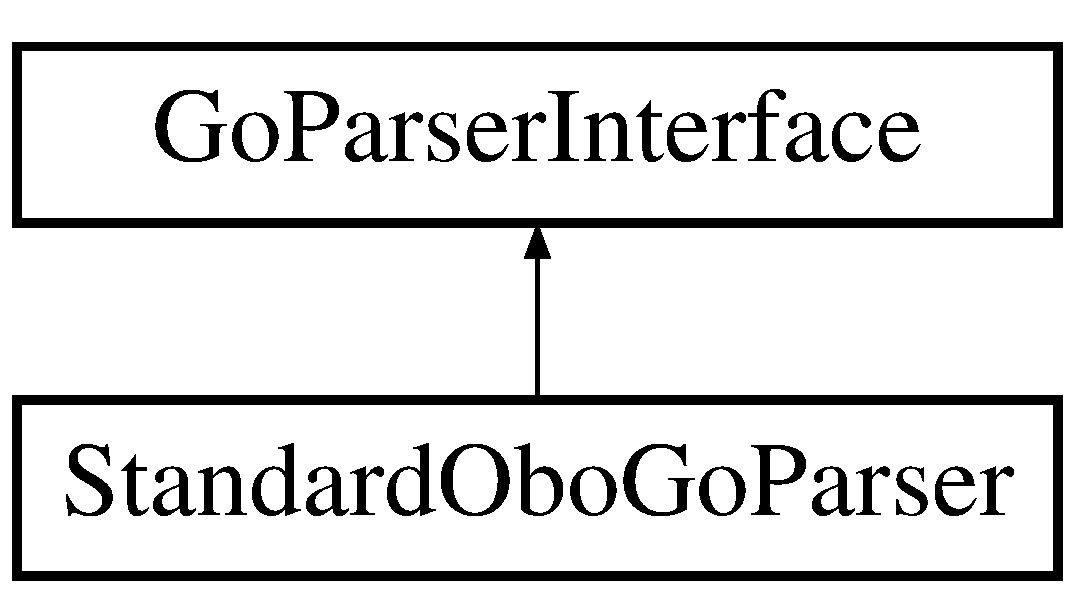
\includegraphics[height=2.000000cm]{classStandardOboGoParser}
\end{center}
\end{figure}
\subsection*{Public Member Functions}
\begin{DoxyCompactItemize}
\item 
\hyperlink{classGoGraph}{Go\+Graph} $\ast$ \hyperlink{classStandardOboGoParser_a4eb0d67f0c78456d1e0a9a3f55294424}{parse\+Go\+File} (std\+::string filename)
\begin{DoxyCompactList}\small\item\em Method to parse the go file, should be an X\+ML file. \end{DoxyCompactList}\item 
bool \hyperlink{classStandardOboGoParser_af6c430101cecf73606ae979d4de6ea7f}{is\+File\+Good} (const std\+::string \&filename)
\begin{DoxyCompactList}\small\item\em A method to test if a file fits the accepted format. \end{DoxyCompactList}\item 
\hyperlink{classGoParserInterface}{Go\+Parser\+Interface} $\ast$ \hyperlink{classStandardOboGoParser_aa4c7c326bf20327645fe6df7d57e3fc3}{clone} ()
\begin{DoxyCompactList}\small\item\em a method to create a new instance of this class for use in a factory \end{DoxyCompactList}\item 
\hyperlink{classStandardOboGoParser_ac7d246fea7b1cad797242405c38f8d4a}{Standard\+Obo\+Go\+Parser} ()
\begin{DoxyCompactList}\small\item\em A parameterized constructor. \end{DoxyCompactList}\end{DoxyCompactItemize}


\subsection{Detailed Description}
A class to parse only is\+\_\+a or part\+\_\+of relationships. 

Implements \hyperlink{classGoParserInterface}{Go\+Parser\+Interface} 

\subsection{Constructor \& Destructor Documentation}
\index{Standard\+Obo\+Go\+Parser@{Standard\+Obo\+Go\+Parser}!Standard\+Obo\+Go\+Parser@{Standard\+Obo\+Go\+Parser}}
\index{Standard\+Obo\+Go\+Parser@{Standard\+Obo\+Go\+Parser}!Standard\+Obo\+Go\+Parser@{Standard\+Obo\+Go\+Parser}}
\subsubsection[{\texorpdfstring{Standard\+Obo\+Go\+Parser()}{StandardOboGoParser()}}]{\setlength{\rightskip}{0pt plus 5cm}Standard\+Obo\+Go\+Parser\+::\+Standard\+Obo\+Go\+Parser (
\begin{DoxyParamCaption}
{}
\end{DoxyParamCaption}
)\hspace{0.3cm}{\ttfamily [inline]}}\hypertarget{classStandardOboGoParser_ac7d246fea7b1cad797242405c38f8d4a}{}\label{classStandardOboGoParser_ac7d246fea7b1cad797242405c38f8d4a}


A parameterized constructor. 

constructor that sets the policy 

\subsection{Member Function Documentation}
\index{Standard\+Obo\+Go\+Parser@{Standard\+Obo\+Go\+Parser}!clone@{clone}}
\index{clone@{clone}!Standard\+Obo\+Go\+Parser@{Standard\+Obo\+Go\+Parser}}
\subsubsection[{\texorpdfstring{clone()}{clone()}}]{\setlength{\rightskip}{0pt plus 5cm}{\bf Go\+Parser\+Interface}$\ast$ Standard\+Obo\+Go\+Parser\+::clone (
\begin{DoxyParamCaption}
{}
\end{DoxyParamCaption}
)\hspace{0.3cm}{\ttfamily [inline]}, {\ttfamily [virtual]}}\hypertarget{classStandardOboGoParser_aa4c7c326bf20327645fe6df7d57e3fc3}{}\label{classStandardOboGoParser_aa4c7c326bf20327645fe6df7d57e3fc3}


a method to create a new instance of this class for use in a factory 

creats a new pointer to the parser, used by the factory for go parsers. 

Implements \hyperlink{classGoParserInterface_a21c4ea01809737ab2975fb71edf6fcd5}{Go\+Parser\+Interface}.

\index{Standard\+Obo\+Go\+Parser@{Standard\+Obo\+Go\+Parser}!is\+File\+Good@{is\+File\+Good}}
\index{is\+File\+Good@{is\+File\+Good}!Standard\+Obo\+Go\+Parser@{Standard\+Obo\+Go\+Parser}}
\subsubsection[{\texorpdfstring{is\+File\+Good(const std\+::string \&filename)}{isFileGood(const std::string &filename)}}]{\setlength{\rightskip}{0pt plus 5cm}bool Standard\+Obo\+Go\+Parser\+::is\+File\+Good (
\begin{DoxyParamCaption}
\item[{const std\+::string \&}]{filename}
\end{DoxyParamCaption}
)\hspace{0.3cm}{\ttfamily [inline]}, {\ttfamily [virtual]}}\hypertarget{classStandardOboGoParser_af6c430101cecf73606ae979d4de6ea7f}{}\label{classStandardOboGoParser_af6c430101cecf73606ae979d4de6ea7f}


A method to test if a file fits the accepted format. 

Returns true if the file matches accepted format, false otherwise 

Implements \hyperlink{classGoParserInterface_a0d2db54063c1ff58a0e15f0187af5aa1}{Go\+Parser\+Interface}.

\index{Standard\+Obo\+Go\+Parser@{Standard\+Obo\+Go\+Parser}!parse\+Go\+File@{parse\+Go\+File}}
\index{parse\+Go\+File@{parse\+Go\+File}!Standard\+Obo\+Go\+Parser@{Standard\+Obo\+Go\+Parser}}
\subsubsection[{\texorpdfstring{parse\+Go\+File(std\+::string filename)}{parseGoFile(std::string filename)}}]{\setlength{\rightskip}{0pt plus 5cm}{\bf Go\+Graph}$\ast$ Standard\+Obo\+Go\+Parser\+::parse\+Go\+File (
\begin{DoxyParamCaption}
\item[{std\+::string}]{filename}
\end{DoxyParamCaption}
)\hspace{0.3cm}{\ttfamily [inline]}, {\ttfamily [virtual]}}\hypertarget{classStandardOboGoParser_a4eb0d67f0c78456d1e0a9a3f55294424}{}\label{classStandardOboGoParser_a4eb0d67f0c78456d1e0a9a3f55294424}


Method to parse the go file, should be an X\+ML file. 

This method will read a Gene Ontology X\+ML file and add only those relationship which are specified to the graph. 

Implements \hyperlink{classGoParserInterface_aefde440e0d5404b9efa2a16a89e09674}{Go\+Parser\+Interface}.



The documentation for this class was generated from the following file\+:\begin{DoxyCompactItemize}
\item 
ggtk/Standard\+Obo\+Go\+Parser.\+hpp\end{DoxyCompactItemize}

\hypertarget{classStandardRelationshipPolicy}{}\section{Standard\+Relationship\+Policy Class Reference}
\label{classStandardRelationshipPolicy}\index{Standard\+Relationship\+Policy@{Standard\+Relationship\+Policy}}


A class to allow only a set of relationships.  




{\ttfamily \#include $<$ggtk/\+Standard\+Relationship\+Policy.\+hpp$>$}

Inheritance diagram for Standard\+Relationship\+Policy\+:\begin{figure}[H]
\begin{center}
\leavevmode
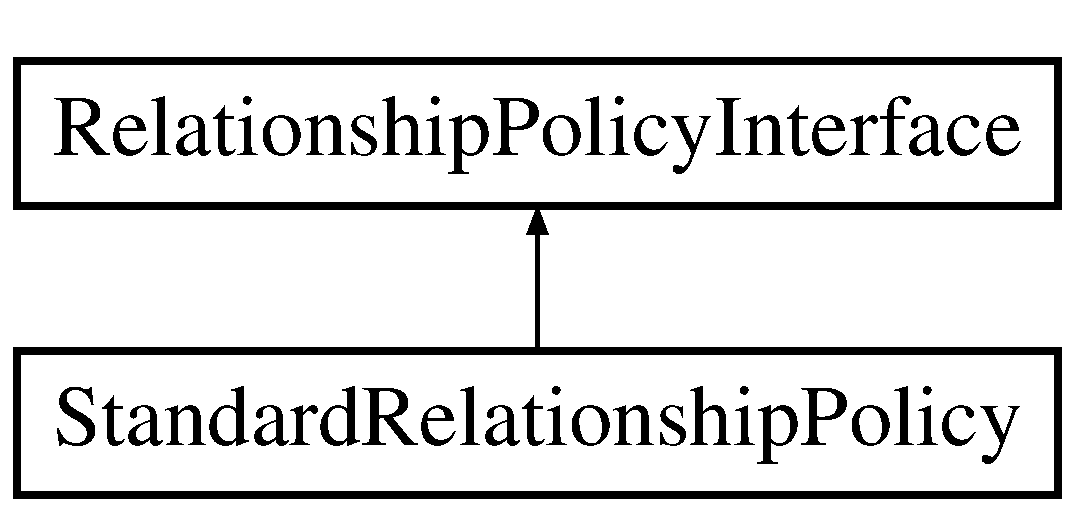
\includegraphics[height=2.000000cm]{classStandardRelationshipPolicy}
\end{center}
\end{figure}
\subsection*{Public Member Functions}
\begin{DoxyCompactItemize}
\item 
\hyperlink{classStandardRelationshipPolicy_a8998d51c3752dfcde0b8931607178c4d}{Standard\+Relationship\+Policy} ()
\begin{DoxyCompactList}\small\item\em A constructor. \end{DoxyCompactList}\item 
\hyperlink{classStandardRelationshipPolicy_af23f42bba1feb00a3b22a96ae17ffacf}{Standard\+Relationship\+Policy} (std\+::vector$<$ \hyperlink{namespaceGO_aaa3905b2e000a8be411da8038827f993}{G\+O\+::\+Relationship} $>$ relationships)
\begin{DoxyCompactList}\small\item\em A parameterized constructor. \end{DoxyCompactList}\item 
bool \hyperlink{classStandardRelationshipPolicy_a75acddf7f5106cacf58f74bd837b03e4}{is\+Allowed} (\hyperlink{namespaceGO_aaa3905b2e000a8be411da8038827f993}{G\+O\+::\+Relationship} relationship)
\begin{DoxyCompactList}\small\item\em a method to test if a relatinoship is allowed or not \end{DoxyCompactList}\end{DoxyCompactItemize}


\subsection{Detailed Description}
A class to allow only a set of relationships. 

A class to allow only certain relationships in the go graph. It uses a set of enums to restric the types of relationships considered in a graph. 

\subsection{Constructor \& Destructor Documentation}
\index{Standard\+Relationship\+Policy@{Standard\+Relationship\+Policy}!Standard\+Relationship\+Policy@{Standard\+Relationship\+Policy}}
\index{Standard\+Relationship\+Policy@{Standard\+Relationship\+Policy}!Standard\+Relationship\+Policy@{Standard\+Relationship\+Policy}}
\subsubsection[{\texorpdfstring{Standard\+Relationship\+Policy()}{StandardRelationshipPolicy()}}]{\setlength{\rightskip}{0pt plus 5cm}Standard\+Relationship\+Policy\+::\+Standard\+Relationship\+Policy (
\begin{DoxyParamCaption}
{}
\end{DoxyParamCaption}
)\hspace{0.3cm}{\ttfamily [inline]}}\hypertarget{classStandardRelationshipPolicy_a8998d51c3752dfcde0b8931607178c4d}{}\label{classStandardRelationshipPolicy_a8998d51c3752dfcde0b8931607178c4d}


A constructor. 

Creates the default(empty) \hyperlink{classStandardRelationshipPolicy}{Standard\+Relationship\+Policy} \index{Standard\+Relationship\+Policy@{Standard\+Relationship\+Policy}!Standard\+Relationship\+Policy@{Standard\+Relationship\+Policy}}
\index{Standard\+Relationship\+Policy@{Standard\+Relationship\+Policy}!Standard\+Relationship\+Policy@{Standard\+Relationship\+Policy}}
\subsubsection[{\texorpdfstring{Standard\+Relationship\+Policy(std\+::vector$<$ G\+O\+::\+Relationship $>$ relationships)}{StandardRelationshipPolicy(std::vector< GO::Relationship > relationships)}}]{\setlength{\rightskip}{0pt plus 5cm}Standard\+Relationship\+Policy\+::\+Standard\+Relationship\+Policy (
\begin{DoxyParamCaption}
\item[{std\+::vector$<$ {\bf G\+O\+::\+Relationship} $>$}]{relationships}
\end{DoxyParamCaption}
)\hspace{0.3cm}{\ttfamily [inline]}}\hypertarget{classStandardRelationshipPolicy_af23f42bba1feb00a3b22a96ae17ffacf}{}\label{classStandardRelationshipPolicy_af23f42bba1feb00a3b22a96ae17ffacf}


A parameterized constructor. 

Creats the \hyperlink{classStandardRelationshipPolicy}{Standard\+Relationship\+Policy} using a list(vector) of relationships to allow 

\subsection{Member Function Documentation}
\index{Standard\+Relationship\+Policy@{Standard\+Relationship\+Policy}!is\+Allowed@{is\+Allowed}}
\index{is\+Allowed@{is\+Allowed}!Standard\+Relationship\+Policy@{Standard\+Relationship\+Policy}}
\subsubsection[{\texorpdfstring{is\+Allowed(\+G\+O\+::\+Relationship relationship)}{isAllowed(GO::Relationship relationship)}}]{\setlength{\rightskip}{0pt plus 5cm}bool Standard\+Relationship\+Policy\+::is\+Allowed (
\begin{DoxyParamCaption}
\item[{{\bf G\+O\+::\+Relationship}}]{relationship}
\end{DoxyParamCaption}
)\hspace{0.3cm}{\ttfamily [inline]}, {\ttfamily [virtual]}}\hypertarget{classStandardRelationshipPolicy_a75acddf7f5106cacf58f74bd837b03e4}{}\label{classStandardRelationshipPolicy_a75acddf7f5106cacf58f74bd837b03e4}


a method to test if a relatinoship is allowed or not 

tests if the relationship is allowed. Overridden to fulfill the \hyperlink{classRelationshipPolicyInterface}{Relationship\+Policy\+Interface} 

Implements \hyperlink{classRelationshipPolicyInterface_ad28012b607e9cf848c791b6a907bb2cb}{Relationship\+Policy\+Interface}.



The documentation for this class was generated from the following file\+:\begin{DoxyCompactItemize}
\item 
ggtk/Standard\+Relationship\+Policy.\+hpp\end{DoxyCompactItemize}

\hypertarget{classStandardXmlGoParser}{}\section{Standard\+Xml\+Go\+Parser Class Reference}
\label{classStandardXmlGoParser}\index{Standard\+Xml\+Go\+Parser@{Standard\+Xml\+Go\+Parser}}


A class to parse only is\+\_\+a or part\+\_\+of relationships.  




{\ttfamily \#include $<$ggtk/\+Standard\+Xml\+Go\+Parser.\+hpp$>$}

Inheritance diagram for Standard\+Xml\+Go\+Parser\+:\begin{figure}[H]
\begin{center}
\leavevmode
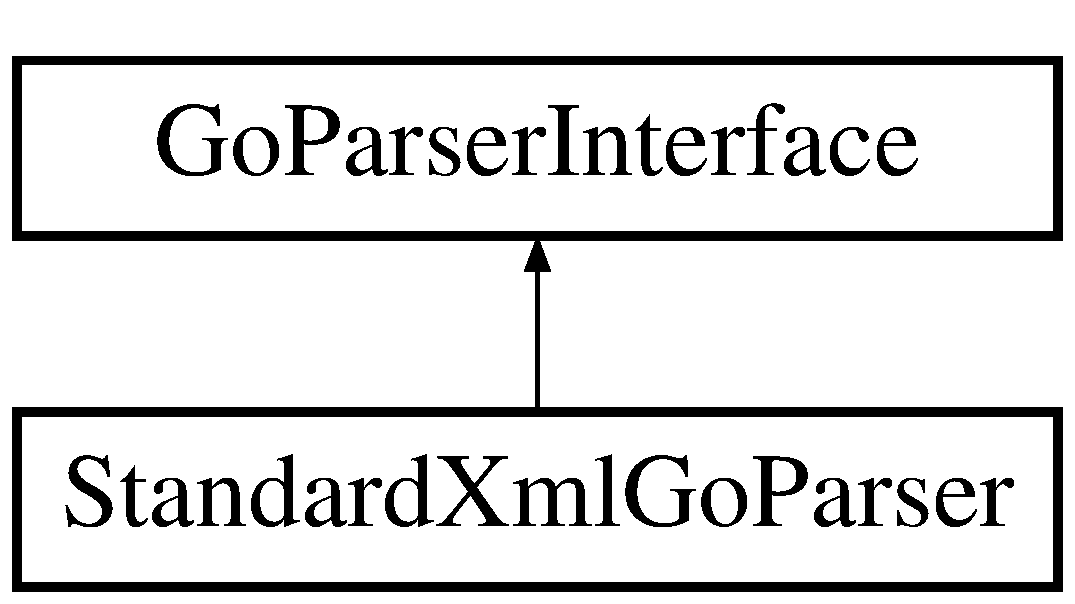
\includegraphics[height=2.000000cm]{classStandardXmlGoParser}
\end{center}
\end{figure}
\subsection*{Public Member Functions}
\begin{DoxyCompactItemize}
\item 
\hyperlink{classGoGraph}{Go\+Graph} $\ast$ \hyperlink{classStandardXmlGoParser_ae56413ab11d1fa8f3870f5bcc262d3f8}{parse\+Go\+File} (std\+::string filename)
\begin{DoxyCompactList}\small\item\em Method to parse the go file, should be an X\+ML file. \end{DoxyCompactList}\item 
bool \hyperlink{classStandardXmlGoParser_a74c344440ef2ce5b30536e09691c92ab}{is\+File\+Good} (const std\+::string \&filename)
\begin{DoxyCompactList}\small\item\em A method to test if a file fits the accepted format. \end{DoxyCompactList}\item 
\hyperlink{classGoParserInterface}{Go\+Parser\+Interface} $\ast$ \hyperlink{classStandardXmlGoParser_ac05cc1de0c2fc74e089169f9baea1f0d}{clone} ()
\begin{DoxyCompactList}\small\item\em a method to create a new instance of this class for use in a factory \end{DoxyCompactList}\item 
\hyperlink{classStandardXmlGoParser_aedda17aae5f75704829b279d2bfe7ac7}{Standard\+Xml\+Go\+Parser} ()
\begin{DoxyCompactList}\small\item\em A parameterized constructor. \end{DoxyCompactList}\end{DoxyCompactItemize}


\subsection{Detailed Description}
A class to parse only is\+\_\+a or part\+\_\+of relationships. 

Implements \hyperlink{classGoParserInterface}{Go\+Parser\+Interface} 

\subsection{Constructor \& Destructor Documentation}
\index{Standard\+Xml\+Go\+Parser@{Standard\+Xml\+Go\+Parser}!Standard\+Xml\+Go\+Parser@{Standard\+Xml\+Go\+Parser}}
\index{Standard\+Xml\+Go\+Parser@{Standard\+Xml\+Go\+Parser}!Standard\+Xml\+Go\+Parser@{Standard\+Xml\+Go\+Parser}}
\subsubsection[{\texorpdfstring{Standard\+Xml\+Go\+Parser()}{StandardXmlGoParser()}}]{\setlength{\rightskip}{0pt plus 5cm}Standard\+Xml\+Go\+Parser\+::\+Standard\+Xml\+Go\+Parser (
\begin{DoxyParamCaption}
{}
\end{DoxyParamCaption}
)\hspace{0.3cm}{\ttfamily [inline]}}\hypertarget{classStandardXmlGoParser_aedda17aae5f75704829b279d2bfe7ac7}{}\label{classStandardXmlGoParser_aedda17aae5f75704829b279d2bfe7ac7}


A parameterized constructor. 

constructor that sets the policy 

\subsection{Member Function Documentation}
\index{Standard\+Xml\+Go\+Parser@{Standard\+Xml\+Go\+Parser}!clone@{clone}}
\index{clone@{clone}!Standard\+Xml\+Go\+Parser@{Standard\+Xml\+Go\+Parser}}
\subsubsection[{\texorpdfstring{clone()}{clone()}}]{\setlength{\rightskip}{0pt plus 5cm}{\bf Go\+Parser\+Interface}$\ast$ Standard\+Xml\+Go\+Parser\+::clone (
\begin{DoxyParamCaption}
{}
\end{DoxyParamCaption}
)\hspace{0.3cm}{\ttfamily [inline]}, {\ttfamily [virtual]}}\hypertarget{classStandardXmlGoParser_ac05cc1de0c2fc74e089169f9baea1f0d}{}\label{classStandardXmlGoParser_ac05cc1de0c2fc74e089169f9baea1f0d}


a method to create a new instance of this class for use in a factory 

creats a new pointer to the parser, used by the factory for go parsers. 

Implements \hyperlink{classGoParserInterface_a21c4ea01809737ab2975fb71edf6fcd5}{Go\+Parser\+Interface}.

\index{Standard\+Xml\+Go\+Parser@{Standard\+Xml\+Go\+Parser}!is\+File\+Good@{is\+File\+Good}}
\index{is\+File\+Good@{is\+File\+Good}!Standard\+Xml\+Go\+Parser@{Standard\+Xml\+Go\+Parser}}
\subsubsection[{\texorpdfstring{is\+File\+Good(const std\+::string \&filename)}{isFileGood(const std::string &filename)}}]{\setlength{\rightskip}{0pt plus 5cm}bool Standard\+Xml\+Go\+Parser\+::is\+File\+Good (
\begin{DoxyParamCaption}
\item[{const std\+::string \&}]{filename}
\end{DoxyParamCaption}
)\hspace{0.3cm}{\ttfamily [inline]}, {\ttfamily [virtual]}}\hypertarget{classStandardXmlGoParser_a74c344440ef2ce5b30536e09691c92ab}{}\label{classStandardXmlGoParser_a74c344440ef2ce5b30536e09691c92ab}


A method to test if a file fits the accepted format. 

Returns true if the file matches accepted format, false otherwise 

Implements \hyperlink{classGoParserInterface_a0d2db54063c1ff58a0e15f0187af5aa1}{Go\+Parser\+Interface}.

\index{Standard\+Xml\+Go\+Parser@{Standard\+Xml\+Go\+Parser}!parse\+Go\+File@{parse\+Go\+File}}
\index{parse\+Go\+File@{parse\+Go\+File}!Standard\+Xml\+Go\+Parser@{Standard\+Xml\+Go\+Parser}}
\subsubsection[{\texorpdfstring{parse\+Go\+File(std\+::string filename)}{parseGoFile(std::string filename)}}]{\setlength{\rightskip}{0pt plus 5cm}{\bf Go\+Graph}$\ast$ Standard\+Xml\+Go\+Parser\+::parse\+Go\+File (
\begin{DoxyParamCaption}
\item[{std\+::string}]{filename}
\end{DoxyParamCaption}
)\hspace{0.3cm}{\ttfamily [inline]}, {\ttfamily [virtual]}}\hypertarget{classStandardXmlGoParser_ae56413ab11d1fa8f3870f5bcc262d3f8}{}\label{classStandardXmlGoParser_ae56413ab11d1fa8f3870f5bcc262d3f8}


Method to parse the go file, should be an X\+ML file. 

This method will read a Gene Ontology X\+ML file and add only those relationship which are specified to the graph. 

Implements \hyperlink{classGoParserInterface_aefde440e0d5404b9efa2a16a89e09674}{Go\+Parser\+Interface}.



The documentation for this class was generated from the following file\+:\begin{DoxyCompactItemize}
\item 
ggtk/Standard\+Xml\+Go\+Parser.\+hpp\end{DoxyCompactItemize}

\hypertarget{classTermDepthMap}{}\section{Term\+Depth\+Map Class Reference}
\label{classTermDepthMap}\index{Term\+Depth\+Map@{Term\+Depth\+Map}}


A class to calculate the depth of a \hyperlink{namespaceGO}{GO} term in the ontology.  




{\ttfamily \#include $<$ggtk/\+Term\+Depth\+Map.\+hpp$>$}

\subsection*{Public Member Functions}
\begin{DoxyCompactItemize}
\item 
\hyperlink{classTermDepthMap_abb4c7ebeedc74ae59a8399de33b48389}{Term\+Depth\+Map} (\hyperlink{classGoGraph}{Go\+Graph} $\ast$graph)
\begin{DoxyCompactList}\small\item\em A parameterized constructor. \end{DoxyCompactList}\item 
\hyperlink{classTermDepthMap_a819c7cb3f26e54e13195a508aff06cdc}{Term\+Depth\+Map} ()
\begin{DoxyCompactList}\small\item\em A default constructor. \end{DoxyCompactList}\item 
\hyperlink{classTermDepthMap_aec4f9d62c638d0f6519d49bb13d96263}{$\sim$\+Term\+Depth\+Map} ()
\begin{DoxyCompactList}\small\item\em A default desctructor. \end{DoxyCompactList}\item 
std\+::vector$<$ double $>$ \hyperlink{classTermDepthMap_acad3e6559688f3338f7d28fffe53f3ab}{get\+Values} ()
\begin{DoxyCompactList}\small\item\em Accessor for probablities vector. \end{DoxyCompactList}\item 
std\+::vector$<$ std\+::string $>$ \hyperlink{classTermDepthMap_a2cc0c96cf91020df4a035f089ef1a608}{get\+Keys} ()
\begin{DoxyCompactList}\small\item\em Function to return all the keys in the map. \end{DoxyCompactList}\item 
bool \hyperlink{classTermDepthMap_a11f5ed887edd0b335ac64171ebecf3f3}{has\+Term} (std\+::string test\+Term)
\begin{DoxyCompactList}\small\item\em Method to test if the id exists in the map. \end{DoxyCompactList}\item 
double \hyperlink{classTermDepthMap_a687255e97647a9afc0a5f0197d0b05c9}{operator\mbox{[}$\,$\mbox{]}} (std\+::string term\+Id)
\begin{DoxyCompactList}\small\item\em Overloaded \mbox{[}\mbox{]} bracket operator to mimic Map. \end{DoxyCompactList}\item 
double \hyperlink{classTermDepthMap_af6ba97e619f7fe0a9e906c6eccfd98fa}{get\+Value} (std\+::string term\+Id)
\begin{DoxyCompactList}\small\item\em Mapping function to return the value mapped by key. \end{DoxyCompactList}\end{DoxyCompactItemize}
\subsection*{Protected Attributes}
\begin{DoxyCompactItemize}
\item 
boost\+::unordered\+\_\+map$<$ std\+::string, std\+::size\+\_\+t $>$ \hyperlink{classTermDepthMap_adf3435b02b709abc108fa8e18e0b73fa}{\+\_\+name\+To\+Index}
\begin{DoxyCompactList}\small\item\em A private map that returns the index of a term. \end{DoxyCompactList}\item 
std\+::vector$<$ double $>$ \hyperlink{classTermDepthMap_af1bc0c6d34c57061de60e771afd76f11}{\+\_\+depths}
\begin{DoxyCompactList}\small\item\em A private list of term depths. \end{DoxyCompactList}\end{DoxyCompactItemize}


\subsection{Detailed Description}
A class to calculate the depth of a \hyperlink{namespaceGO}{GO} term in the ontology. 

This class provides a map that returns the depth of a \hyperlink{namespaceGO}{GO} term. This method is used in graph and edge based similarity methods to calculate a node\textquotesingle{}s depth 

\subsection{Constructor \& Destructor Documentation}
\index{Term\+Depth\+Map@{Term\+Depth\+Map}!Term\+Depth\+Map@{Term\+Depth\+Map}}
\index{Term\+Depth\+Map@{Term\+Depth\+Map}!Term\+Depth\+Map@{Term\+Depth\+Map}}
\subsubsection[{\texorpdfstring{Term\+Depth\+Map(\+Go\+Graph $\ast$graph)}{TermDepthMap(GoGraph *graph)}}]{\setlength{\rightskip}{0pt plus 5cm}Term\+Depth\+Map\+::\+Term\+Depth\+Map (
\begin{DoxyParamCaption}
\item[{{\bf Go\+Graph} $\ast$}]{graph}
\end{DoxyParamCaption}
)\hspace{0.3cm}{\ttfamily [inline]}}\hypertarget{classTermDepthMap_abb4c7ebeedc74ae59a8399de33b48389}{}\label{classTermDepthMap_abb4c7ebeedc74ae59a8399de33b48389}


A parameterized constructor. 

This constructor takes pointers to \hyperlink{classGoGraph}{Go\+Graph} and \hyperlink{classAnnotationData}{Annotation\+Data} objects. Only the parameterized construtor is allowed to ensure these objects are created with valid parameters. \index{Term\+Depth\+Map@{Term\+Depth\+Map}!Term\+Depth\+Map@{Term\+Depth\+Map}}
\index{Term\+Depth\+Map@{Term\+Depth\+Map}!Term\+Depth\+Map@{Term\+Depth\+Map}}
\subsubsection[{\texorpdfstring{Term\+Depth\+Map()}{TermDepthMap()}}]{\setlength{\rightskip}{0pt plus 5cm}Term\+Depth\+Map\+::\+Term\+Depth\+Map (
\begin{DoxyParamCaption}
{}
\end{DoxyParamCaption}
)\hspace{0.3cm}{\ttfamily [inline]}}\hypertarget{classTermDepthMap_a819c7cb3f26e54e13195a508aff06cdc}{}\label{classTermDepthMap_a819c7cb3f26e54e13195a508aff06cdc}


A default constructor. 

This constructor initialized the storage structures. Should not be used. \index{Term\+Depth\+Map@{Term\+Depth\+Map}!````~Term\+Depth\+Map@{$\sim$\+Term\+Depth\+Map}}
\index{````~Term\+Depth\+Map@{$\sim$\+Term\+Depth\+Map}!Term\+Depth\+Map@{Term\+Depth\+Map}}
\subsubsection[{\texorpdfstring{$\sim$\+Term\+Depth\+Map()}{~TermDepthMap()}}]{\setlength{\rightskip}{0pt plus 5cm}Term\+Depth\+Map\+::$\sim$\+Term\+Depth\+Map (
\begin{DoxyParamCaption}
{}
\end{DoxyParamCaption}
)\hspace{0.3cm}{\ttfamily [inline]}}\hypertarget{classTermDepthMap_aec4f9d62c638d0f6519d49bb13d96263}{}\label{classTermDepthMap_aec4f9d62c638d0f6519d49bb13d96263}


A default desctructor. 

This desctructor clears the containters 

\subsection{Member Function Documentation}
\index{Term\+Depth\+Map@{Term\+Depth\+Map}!get\+Keys@{get\+Keys}}
\index{get\+Keys@{get\+Keys}!Term\+Depth\+Map@{Term\+Depth\+Map}}
\subsubsection[{\texorpdfstring{get\+Keys()}{getKeys()}}]{\setlength{\rightskip}{0pt plus 5cm}std\+::vector$<$std\+::string$>$ Term\+Depth\+Map\+::get\+Keys (
\begin{DoxyParamCaption}
{}
\end{DoxyParamCaption}
)\hspace{0.3cm}{\ttfamily [inline]}}\hypertarget{classTermDepthMap_a2cc0c96cf91020df4a035f089ef1a608}{}\label{classTermDepthMap_a2cc0c96cf91020df4a035f089ef1a608}


Function to return all the keys in the map. 

Returns all valid keys in the map. \index{Term\+Depth\+Map@{Term\+Depth\+Map}!get\+Value@{get\+Value}}
\index{get\+Value@{get\+Value}!Term\+Depth\+Map@{Term\+Depth\+Map}}
\subsubsection[{\texorpdfstring{get\+Value(std\+::string term\+Id)}{getValue(std::string termId)}}]{\setlength{\rightskip}{0pt plus 5cm}double Term\+Depth\+Map\+::get\+Value (
\begin{DoxyParamCaption}
\item[{std\+::string}]{term\+Id}
\end{DoxyParamCaption}
)\hspace{0.3cm}{\ttfamily [inline]}}\hypertarget{classTermDepthMap_af6ba97e619f7fe0a9e906c6eccfd98fa}{}\label{classTermDepthMap_af6ba97e619f7fe0a9e906c6eccfd98fa}


Mapping function to return the value mapped by key. 

Get the value mapped by the given key. A specified function for the \mbox{[}\mbox{]} operator \index{Term\+Depth\+Map@{Term\+Depth\+Map}!get\+Values@{get\+Values}}
\index{get\+Values@{get\+Values}!Term\+Depth\+Map@{Term\+Depth\+Map}}
\subsubsection[{\texorpdfstring{get\+Values()}{getValues()}}]{\setlength{\rightskip}{0pt plus 5cm}std\+::vector$<$double$>$ Term\+Depth\+Map\+::get\+Values (
\begin{DoxyParamCaption}
{}
\end{DoxyParamCaption}
)\hspace{0.3cm}{\ttfamily [inline]}}\hypertarget{classTermDepthMap_acad3e6559688f3338f7d28fffe53f3ab}{}\label{classTermDepthMap_acad3e6559688f3338f7d28fffe53f3ab}


Accessor for probablities vector. 

Get the vector of values \index{Term\+Depth\+Map@{Term\+Depth\+Map}!has\+Term@{has\+Term}}
\index{has\+Term@{has\+Term}!Term\+Depth\+Map@{Term\+Depth\+Map}}
\subsubsection[{\texorpdfstring{has\+Term(std\+::string test\+Term)}{hasTerm(std::string testTerm)}}]{\setlength{\rightskip}{0pt plus 5cm}bool Term\+Depth\+Map\+::has\+Term (
\begin{DoxyParamCaption}
\item[{std\+::string}]{test\+Term}
\end{DoxyParamCaption}
)\hspace{0.3cm}{\ttfamily [inline]}}\hypertarget{classTermDepthMap_a11f5ed887edd0b335ac64171ebecf3f3}{}\label{classTermDepthMap_a11f5ed887edd0b335ac64171ebecf3f3}


Method to test if the id exists in the map. 

Return true the id is found, false if not \index{Term\+Depth\+Map@{Term\+Depth\+Map}!operator\mbox{[}$\,$\mbox{]}@{operator[]}}
\index{operator\mbox{[}$\,$\mbox{]}@{operator[]}!Term\+Depth\+Map@{Term\+Depth\+Map}}
\subsubsection[{\texorpdfstring{operator[](std\+::string term\+Id)}{operator[](std::string termId)}}]{\setlength{\rightskip}{0pt plus 5cm}double Term\+Depth\+Map\+::operator\mbox{[}$\,$\mbox{]} (
\begin{DoxyParamCaption}
\item[{std\+::string}]{term\+Id}
\end{DoxyParamCaption}
)\hspace{0.3cm}{\ttfamily [inline]}}\hypertarget{classTermDepthMap_a687255e97647a9afc0a5f0197d0b05c9}{}\label{classTermDepthMap_a687255e97647a9afc0a5f0197d0b05c9}


Overloaded \mbox{[}\mbox{]} bracket operator to mimic Map. 

This defines a bracket operator to access the data inside of the map. This is done to mimic the behavior of the map class 

\subsection{Member Data Documentation}
\index{Term\+Depth\+Map@{Term\+Depth\+Map}!\+\_\+depths@{\+\_\+depths}}
\index{\+\_\+depths@{\+\_\+depths}!Term\+Depth\+Map@{Term\+Depth\+Map}}
\subsubsection[{\texorpdfstring{\+\_\+depths}{_depths}}]{\setlength{\rightskip}{0pt plus 5cm}std\+::vector$<$double$>$ Term\+Depth\+Map\+::\+\_\+depths\hspace{0.3cm}{\ttfamily [protected]}}\hypertarget{classTermDepthMap_af1bc0c6d34c57061de60e771afd76f11}{}\label{classTermDepthMap_af1bc0c6d34c57061de60e771afd76f11}


A private list of term depths. 

This vector of doubles holds the depth for each term \index{Term\+Depth\+Map@{Term\+Depth\+Map}!\+\_\+name\+To\+Index@{\+\_\+name\+To\+Index}}
\index{\+\_\+name\+To\+Index@{\+\_\+name\+To\+Index}!Term\+Depth\+Map@{Term\+Depth\+Map}}
\subsubsection[{\texorpdfstring{\+\_\+name\+To\+Index}{_nameToIndex}}]{\setlength{\rightskip}{0pt plus 5cm}boost\+::unordered\+\_\+map$<$std\+::string,std\+::size\+\_\+t$>$ Term\+Depth\+Map\+::\+\_\+name\+To\+Index\hspace{0.3cm}{\ttfamily [protected]}}\hypertarget{classTermDepthMap_adf3435b02b709abc108fa8e18e0b73fa}{}\label{classTermDepthMap_adf3435b02b709abc108fa8e18e0b73fa}


A private map that returns the index of a term. 

This map takes string term ids and returns the index for annotation count access. 

The documentation for this class was generated from the following file\+:\begin{DoxyCompactItemize}
\item 
ggtk/Term\+Depth\+Map.\+hpp\end{DoxyCompactItemize}

\hypertarget{classTermInformationContentMap}{}\section{Term\+Information\+Content\+Map Class Reference}
\label{classTermInformationContentMap}\index{Term\+Information\+Content\+Map@{Term\+Information\+Content\+Map}}


A class to calculate the information content of a \hyperlink{namespaceGO}{GO} term.  




{\ttfamily \#include $<$ggtk/\+Term\+Information\+Content\+Map.\+hpp$>$}

Inheritance diagram for Term\+Information\+Content\+Map\+:\begin{figure}[H]
\begin{center}
\leavevmode
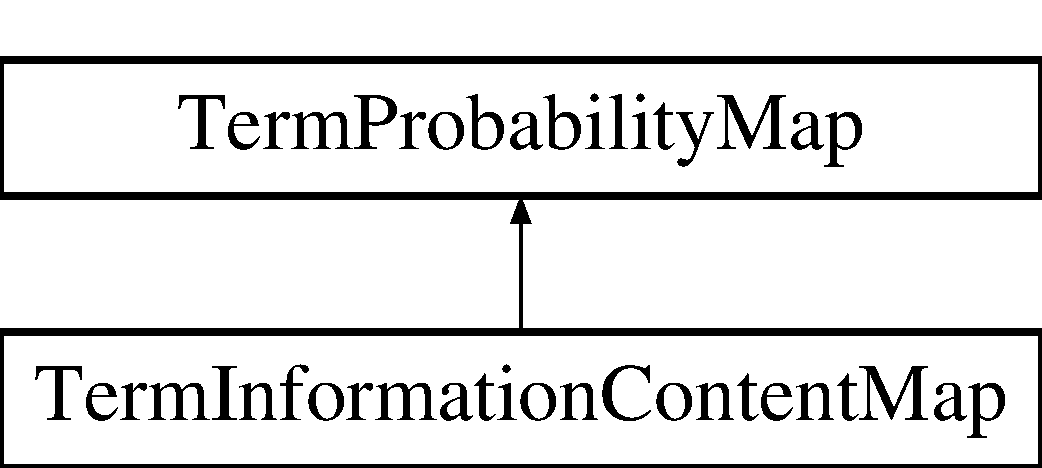
\includegraphics[height=2.000000cm]{classTermInformationContentMap}
\end{center}
\end{figure}
\subsection*{Public Member Functions}
\begin{DoxyCompactItemize}
\item 
\hyperlink{classTermInformationContentMap_ae58d9e3773eff919841e2de522ececd1}{Term\+Information\+Content\+Map} (\hyperlink{classGoGraph}{Go\+Graph} $\ast$graph, \hyperlink{classAnnotationData}{Annotation\+Data} $\ast$anno\+Data)
\begin{DoxyCompactList}\small\item\em A parameterized constructor. \end{DoxyCompactList}\item 
double \hyperlink{classTermInformationContentMap_a082c021a27478403aad9bb99c0e975e6}{bad\+Id\+Value} ()
\begin{DoxyCompactList}\small\item\em Return a default value for a term that does not exist. \end{DoxyCompactList}\item 
\hyperlink{classTermInformationContentMap_a86494db712efa761fb671d51a6902c25}{Term\+Information\+Content\+Map} ()
\begin{DoxyCompactList}\small\item\em A default constructor. \end{DoxyCompactList}\end{DoxyCompactItemize}
\subsection*{Additional Inherited Members}


\subsection{Detailed Description}
A class to calculate the information content of a \hyperlink{namespaceGO}{GO} term. 

This class provides a map that returns the information content of a \hyperlink{namespaceGO}{GO} term. This class is used by Information Content methods. 

\subsection{Constructor \& Destructor Documentation}
\index{Term\+Information\+Content\+Map@{Term\+Information\+Content\+Map}!Term\+Information\+Content\+Map@{Term\+Information\+Content\+Map}}
\index{Term\+Information\+Content\+Map@{Term\+Information\+Content\+Map}!Term\+Information\+Content\+Map@{Term\+Information\+Content\+Map}}
\subsubsection[{\texorpdfstring{Term\+Information\+Content\+Map(\+Go\+Graph $\ast$graph, Annotation\+Data $\ast$anno\+Data)}{TermInformationContentMap(GoGraph *graph, AnnotationData *annoData)}}]{\setlength{\rightskip}{0pt plus 5cm}Term\+Information\+Content\+Map\+::\+Term\+Information\+Content\+Map (
\begin{DoxyParamCaption}
\item[{{\bf Go\+Graph} $\ast$}]{graph, }
\item[{{\bf Annotation\+Data} $\ast$}]{anno\+Data}
\end{DoxyParamCaption}
)\hspace{0.3cm}{\ttfamily [inline]}}\hypertarget{classTermInformationContentMap_ae58d9e3773eff919841e2de522ececd1}{}\label{classTermInformationContentMap_ae58d9e3773eff919841e2de522ececd1}


A parameterized constructor. 

This constructor takes pointers to \hyperlink{classGoGraph}{Go\+Graph} and \hyperlink{classAnnotationData}{Annotation\+Data} objects. Only the parameterized construtor is allowed to ensure these objects are created with valid parameters. This constructor relies on the \hyperlink{classTermProbabilityMap}{Term\+Probability\+Map}. \index{Term\+Information\+Content\+Map@{Term\+Information\+Content\+Map}!Term\+Information\+Content\+Map@{Term\+Information\+Content\+Map}}
\index{Term\+Information\+Content\+Map@{Term\+Information\+Content\+Map}!Term\+Information\+Content\+Map@{Term\+Information\+Content\+Map}}
\subsubsection[{\texorpdfstring{Term\+Information\+Content\+Map()}{TermInformationContentMap()}}]{\setlength{\rightskip}{0pt plus 5cm}Term\+Information\+Content\+Map\+::\+Term\+Information\+Content\+Map (
\begin{DoxyParamCaption}
{}
\end{DoxyParamCaption}
)\hspace{0.3cm}{\ttfamily [inline]}}\hypertarget{classTermInformationContentMap_a86494db712efa761fb671d51a6902c25}{}\label{classTermInformationContentMap_a86494db712efa761fb671d51a6902c25}


A default constructor. 

This constructor creates an empty IC map. Should not be used. 

\subsection{Member Function Documentation}
\index{Term\+Information\+Content\+Map@{Term\+Information\+Content\+Map}!bad\+Id\+Value@{bad\+Id\+Value}}
\index{bad\+Id\+Value@{bad\+Id\+Value}!Term\+Information\+Content\+Map@{Term\+Information\+Content\+Map}}
\subsubsection[{\texorpdfstring{bad\+Id\+Value()}{badIdValue()}}]{\setlength{\rightskip}{0pt plus 5cm}double Term\+Information\+Content\+Map\+::bad\+Id\+Value (
\begin{DoxyParamCaption}
{}
\end{DoxyParamCaption}
)\hspace{0.3cm}{\ttfamily [inline]}, {\ttfamily [virtual]}}\hypertarget{classTermInformationContentMap_a082c021a27478403aad9bb99c0e975e6}{}\label{classTermInformationContentMap_a082c021a27478403aad9bb99c0e975e6}


Return a default value for a term that does not exist. 

A value to return if the term is not found (does not exist in the map). Returns informaiton content 0. This may not be the ideal behavior. 

Reimplemented from \hyperlink{classTermProbabilityMap_adfeb9edb261c639cceae797cceb88d35}{Term\+Probability\+Map}.



The documentation for this class was generated from the following file\+:\begin{DoxyCompactItemize}
\item 
ggtk/Term\+Information\+Content\+Map.\+hpp\end{DoxyCompactItemize}

\hypertarget{classTermProbabilityMap}{}\section{Term\+Probability\+Map Class Reference}
\label{classTermProbabilityMap}\index{Term\+Probability\+Map@{Term\+Probability\+Map}}


A class to calculate the probability of a \hyperlink{namespaceGO}{GO} term.  




{\ttfamily \#include $<$ggtk/\+Term\+Probability\+Map.\+hpp$>$}

Inheritance diagram for Term\+Probability\+Map\+:\begin{figure}[H]
\begin{center}
\leavevmode
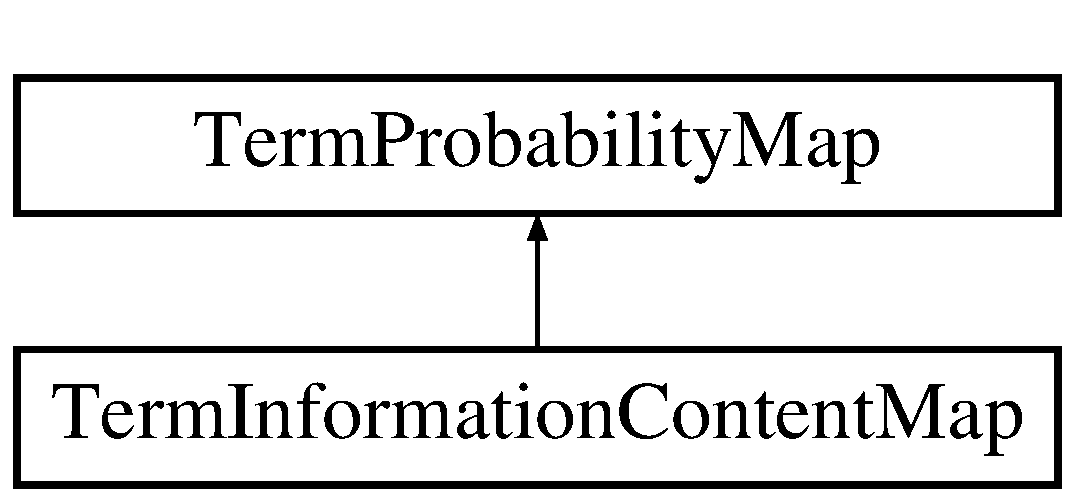
\includegraphics[height=2.000000cm]{classTermProbabilityMap}
\end{center}
\end{figure}
\subsection*{Classes}
\begin{DoxyCompactItemize}
\item 
class \hyperlink{classTermProbabilityMap_1_1dfs__cumulative__annotations__visitor}{dfs\+\_\+cumulative\+\_\+annotations\+\_\+visitor}
\begin{DoxyCompactList}\small\item\em Depth first search boost visitor. \end{DoxyCompactList}\end{DoxyCompactItemize}
\subsection*{Public Member Functions}
\begin{DoxyCompactItemize}
\item 
\hyperlink{classTermProbabilityMap_a44b7437af56eecc461983a70b5e0e5f3}{Term\+Probability\+Map} (\hyperlink{classGoGraph}{Go\+Graph} $\ast$graph, \hyperlink{classAnnotationData}{Annotation\+Data} $\ast$anno\+Data)
\begin{DoxyCompactList}\small\item\em A parameterized constructor. \end{DoxyCompactList}\item 
\hyperlink{classTermProbabilityMap_a3bddf2e9aa81dd0e1f40aa1dc4ff2713}{Term\+Probability\+Map} ()
\begin{DoxyCompactList}\small\item\em A default constructor. \end{DoxyCompactList}\item 
\hyperlink{classTermProbabilityMap_a9e409916fa3c75fb7900a3f83d7c55b9}{$\sim$\+Term\+Probability\+Map} ()
\begin{DoxyCompactList}\small\item\em A default desctructor. \end{DoxyCompactList}\item 
std\+::vector$<$ double $>$ \hyperlink{classTermProbabilityMap_ae960575c867ee0954b6beee3c10b280d}{get\+Values} ()
\begin{DoxyCompactList}\small\item\em Accessor for probablities vector. \end{DoxyCompactList}\item 
std\+::vector$<$ std\+::string $>$ \hyperlink{classTermProbabilityMap_a207545a1c1703d8be20fc0847156f2cc}{get\+Keys} ()
\begin{DoxyCompactList}\small\item\em Function to return all the keys in the map. \end{DoxyCompactList}\item 
bool \hyperlink{classTermProbabilityMap_a14087f464ea33bf0247d6034e9ee2e9f}{has\+Term} (const std\+::string \&test\+Term)
\begin{DoxyCompactList}\small\item\em Method to test if the id exists in the map. \end{DoxyCompactList}\item 
virtual double \hyperlink{classTermProbabilityMap_adfeb9edb261c639cceae797cceb88d35}{bad\+Id\+Value} ()
\begin{DoxyCompactList}\small\item\em Return a default value for a term that does not exist. \end{DoxyCompactList}\item 
double \hyperlink{classTermProbabilityMap_acd472ef3c011377e6b9bdb01a60e84e1}{operator\mbox{[}$\,$\mbox{]}} (std\+::string term\+Id)
\begin{DoxyCompactList}\small\item\em Overloaded \mbox{[}\mbox{]} bracket operator to mimic Map. \end{DoxyCompactList}\item 
double \hyperlink{classTermProbabilityMap_a4ef29e6a25cb1b781c5a0b05b9b82ebf}{get\+Value} (std\+::string term\+Id)
\begin{DoxyCompactList}\small\item\em Mapping function to return the value mapped by key. \end{DoxyCompactList}\item 
double \hyperlink{classTermProbabilityMap_aa0cbaada30cf4fe8f7bf55acdfcbe7aa}{get\+Min\+BP} ()
\begin{DoxyCompactList}\small\item\em Get the specific minimum probability for BP. \end{DoxyCompactList}\item 
double \hyperlink{classTermProbabilityMap_af23163c0122e7745b6581eda91a72809}{get\+Min\+MF} ()
\begin{DoxyCompactList}\small\item\em Get the specific minimum probability for MF. \end{DoxyCompactList}\item 
double \hyperlink{classTermProbabilityMap_aa74c8e413fa1cce4d6528ccfad32efad}{get\+Min\+CC} ()
\begin{DoxyCompactList}\small\item\em Get the specific minimum probability for CC. \end{DoxyCompactList}\end{DoxyCompactItemize}
\subsection*{Protected Attributes}
\begin{DoxyCompactItemize}
\item 
boost\+::unordered\+\_\+map$<$ std\+::string, std\+::size\+\_\+t $>$ \hyperlink{classTermProbabilityMap_af94f810eb87afe5c7bddb14d19735e86}{\+\_\+name\+To\+Index}
\begin{DoxyCompactList}\small\item\em A private map that returns the index of a term. \end{DoxyCompactList}\item 
std\+::vector$<$ double $>$ \hyperlink{classTermProbabilityMap_a1cbbbb63e115e69359e2d4fb65be6227}{\+\_\+probabilities}
\begin{DoxyCompactList}\small\item\em A private list of term probabilities. \end{DoxyCompactList}\item 
bool \hyperlink{classTermProbabilityMap_a7cb93d7a55e3002065838f16a1f8c282}{\+\_\+is\+Single\+Anno\+Min}
\begin{DoxyCompactList}\small\item\em A flag designating the minimum policy. \end{DoxyCompactList}\item 
double \hyperlink{classTermProbabilityMap_a1bdc8b5b73d1686abbaf1f5dd698d500}{\+\_\+bp\+\_\+normalization\+\_\+min\+\_\+1anno}
\begin{DoxyCompactList}\small\item\em Normalization factor for calculating normalized simialrites Biological Process. \end{DoxyCompactList}\item 
double \hyperlink{classTermProbabilityMap_aedd2c51ffd41664ef2dd714bde4aa5fa}{\+\_\+bp\+\_\+normalization\+\_\+min\+\_\+min\+Anno}
\begin{DoxyCompactList}\small\item\em Normalization factor for calculating normalized simialrites for Biological Process. \end{DoxyCompactList}\item 
double \hyperlink{classTermProbabilityMap_a9c240b82c9cec69d2d777b3a95d81891}{\+\_\+mf\+\_\+normalization\+\_\+min\+\_\+1anno}
\begin{DoxyCompactList}\small\item\em Normalization factor for calculating normalized simialrites Molecular Function. \end{DoxyCompactList}\item 
double \hyperlink{classTermProbabilityMap_adfbe0bba2e300c32941c7d83f8e3febb}{\+\_\+mf\+\_\+normalization\+\_\+min\+\_\+min\+Anno}
\begin{DoxyCompactList}\small\item\em Normalization factor for calculating normalized simialrites for Molecular Function. \end{DoxyCompactList}\item 
double \hyperlink{classTermProbabilityMap_a8c16045a4e738758ff5510c04da20290}{\+\_\+cc\+\_\+normalization\+\_\+min\+\_\+1anno}
\begin{DoxyCompactList}\small\item\em Normalization factor for calculating normalized simialrites Cellular Component. \end{DoxyCompactList}\item 
double \hyperlink{classTermProbabilityMap_a5a665cb81ee03caca135a9a36cd544a1}{\+\_\+cc\+\_\+normalization\+\_\+min\+\_\+min\+Anno}
\begin{DoxyCompactList}\small\item\em Normalization factor for calculating normalized simialrites for Cellular Component. \end{DoxyCompactList}\end{DoxyCompactItemize}


\subsection{Detailed Description}
A class to calculate the probability of a \hyperlink{namespaceGO}{GO} term. 

This class provides a map that returns the probability of \hyperlink{namespaceGO}{GO} term. This class is used by Information Content methods to determine the prior probability of a term give an instance of \hyperlink{classAnnotationData}{Annotation\+Data}. 

\subsection{Constructor \& Destructor Documentation}
\index{Term\+Probability\+Map@{Term\+Probability\+Map}!Term\+Probability\+Map@{Term\+Probability\+Map}}
\index{Term\+Probability\+Map@{Term\+Probability\+Map}!Term\+Probability\+Map@{Term\+Probability\+Map}}
\subsubsection[{\texorpdfstring{Term\+Probability\+Map(\+Go\+Graph $\ast$graph, Annotation\+Data $\ast$anno\+Data)}{TermProbabilityMap(GoGraph *graph, AnnotationData *annoData)}}]{\setlength{\rightskip}{0pt plus 5cm}Term\+Probability\+Map\+::\+Term\+Probability\+Map (
\begin{DoxyParamCaption}
\item[{{\bf Go\+Graph} $\ast$}]{graph, }
\item[{{\bf Annotation\+Data} $\ast$}]{anno\+Data}
\end{DoxyParamCaption}
)\hspace{0.3cm}{\ttfamily [inline]}}\hypertarget{classTermProbabilityMap_a44b7437af56eecc461983a70b5e0e5f3}{}\label{classTermProbabilityMap_a44b7437af56eecc461983a70b5e0e5f3}


A parameterized constructor. 

This constructor takes pointers to \hyperlink{classGoGraph}{Go\+Graph} and \hyperlink{classAnnotationData}{Annotation\+Data} objects. Only the parameterized construtor is allowed to ensure these objects are created with valid parameters. \index{Term\+Probability\+Map@{Term\+Probability\+Map}!Term\+Probability\+Map@{Term\+Probability\+Map}}
\index{Term\+Probability\+Map@{Term\+Probability\+Map}!Term\+Probability\+Map@{Term\+Probability\+Map}}
\subsubsection[{\texorpdfstring{Term\+Probability\+Map()}{TermProbabilityMap()}}]{\setlength{\rightskip}{0pt plus 5cm}Term\+Probability\+Map\+::\+Term\+Probability\+Map (
\begin{DoxyParamCaption}
{}
\end{DoxyParamCaption}
)\hspace{0.3cm}{\ttfamily [inline]}}\hypertarget{classTermProbabilityMap_a3bddf2e9aa81dd0e1f40aa1dc4ff2713}{}\label{classTermProbabilityMap_a3bddf2e9aa81dd0e1f40aa1dc4ff2713}


A default constructor. 

This constructor initialized the storage structures. Should not be used. \index{Term\+Probability\+Map@{Term\+Probability\+Map}!````~Term\+Probability\+Map@{$\sim$\+Term\+Probability\+Map}}
\index{````~Term\+Probability\+Map@{$\sim$\+Term\+Probability\+Map}!Term\+Probability\+Map@{Term\+Probability\+Map}}
\subsubsection[{\texorpdfstring{$\sim$\+Term\+Probability\+Map()}{~TermProbabilityMap()}}]{\setlength{\rightskip}{0pt plus 5cm}Term\+Probability\+Map\+::$\sim$\+Term\+Probability\+Map (
\begin{DoxyParamCaption}
{}
\end{DoxyParamCaption}
)\hspace{0.3cm}{\ttfamily [inline]}}\hypertarget{classTermProbabilityMap_a9e409916fa3c75fb7900a3f83d7c55b9}{}\label{classTermProbabilityMap_a9e409916fa3c75fb7900a3f83d7c55b9}


A default desctructor. 

This desctructor clears the containters 

\subsection{Member Function Documentation}
\index{Term\+Probability\+Map@{Term\+Probability\+Map}!bad\+Id\+Value@{bad\+Id\+Value}}
\index{bad\+Id\+Value@{bad\+Id\+Value}!Term\+Probability\+Map@{Term\+Probability\+Map}}
\subsubsection[{\texorpdfstring{bad\+Id\+Value()}{badIdValue()}}]{\setlength{\rightskip}{0pt plus 5cm}virtual double Term\+Probability\+Map\+::bad\+Id\+Value (
\begin{DoxyParamCaption}
{}
\end{DoxyParamCaption}
)\hspace{0.3cm}{\ttfamily [inline]}, {\ttfamily [virtual]}}\hypertarget{classTermProbabilityMap_adfeb9edb261c639cceae797cceb88d35}{}\label{classTermProbabilityMap_adfeb9edb261c639cceae797cceb88d35}


Return a default value for a term that does not exist. 

A value to return if the term is not found (does not exist in the map). Returns probability 1 or certanty. This may not be the ideal behavior. 

Reimplemented in \hyperlink{classTermInformationContentMap_a082c021a27478403aad9bb99c0e975e6}{Term\+Information\+Content\+Map}.

\index{Term\+Probability\+Map@{Term\+Probability\+Map}!get\+Keys@{get\+Keys}}
\index{get\+Keys@{get\+Keys}!Term\+Probability\+Map@{Term\+Probability\+Map}}
\subsubsection[{\texorpdfstring{get\+Keys()}{getKeys()}}]{\setlength{\rightskip}{0pt plus 5cm}std\+::vector$<$std\+::string$>$ Term\+Probability\+Map\+::get\+Keys (
\begin{DoxyParamCaption}
{}
\end{DoxyParamCaption}
)\hspace{0.3cm}{\ttfamily [inline]}}\hypertarget{classTermProbabilityMap_a207545a1c1703d8be20fc0847156f2cc}{}\label{classTermProbabilityMap_a207545a1c1703d8be20fc0847156f2cc}


Function to return all the keys in the map. 

Returns all valid keys in the map. \index{Term\+Probability\+Map@{Term\+Probability\+Map}!get\+Min\+BP@{get\+Min\+BP}}
\index{get\+Min\+BP@{get\+Min\+BP}!Term\+Probability\+Map@{Term\+Probability\+Map}}
\subsubsection[{\texorpdfstring{get\+Min\+B\+P()}{getMinBP()}}]{\setlength{\rightskip}{0pt plus 5cm}double Term\+Probability\+Map\+::get\+Min\+BP (
\begin{DoxyParamCaption}
{}
\end{DoxyParamCaption}
)\hspace{0.3cm}{\ttfamily [inline]}}\hypertarget{classTermProbabilityMap_aa0cbaada30cf4fe8f7bf55acdfcbe7aa}{}\label{classTermProbabilityMap_aa0cbaada30cf4fe8f7bf55acdfcbe7aa}


Get the specific minimum probability for BP. 

This function returns the minimum probablity for the bp ontology \index{Term\+Probability\+Map@{Term\+Probability\+Map}!get\+Min\+CC@{get\+Min\+CC}}
\index{get\+Min\+CC@{get\+Min\+CC}!Term\+Probability\+Map@{Term\+Probability\+Map}}
\subsubsection[{\texorpdfstring{get\+Min\+C\+C()}{getMinCC()}}]{\setlength{\rightskip}{0pt plus 5cm}double Term\+Probability\+Map\+::get\+Min\+CC (
\begin{DoxyParamCaption}
{}
\end{DoxyParamCaption}
)\hspace{0.3cm}{\ttfamily [inline]}}\hypertarget{classTermProbabilityMap_aa74c8e413fa1cce4d6528ccfad32efad}{}\label{classTermProbabilityMap_aa74c8e413fa1cce4d6528ccfad32efad}


Get the specific minimum probability for CC. 

This function returns the minimum probablity for the cc ontology \index{Term\+Probability\+Map@{Term\+Probability\+Map}!get\+Min\+MF@{get\+Min\+MF}}
\index{get\+Min\+MF@{get\+Min\+MF}!Term\+Probability\+Map@{Term\+Probability\+Map}}
\subsubsection[{\texorpdfstring{get\+Min\+M\+F()}{getMinMF()}}]{\setlength{\rightskip}{0pt plus 5cm}double Term\+Probability\+Map\+::get\+Min\+MF (
\begin{DoxyParamCaption}
{}
\end{DoxyParamCaption}
)\hspace{0.3cm}{\ttfamily [inline]}}\hypertarget{classTermProbabilityMap_af23163c0122e7745b6581eda91a72809}{}\label{classTermProbabilityMap_af23163c0122e7745b6581eda91a72809}


Get the specific minimum probability for MF. 

This function returns the minimum probablity for the mf ontology \index{Term\+Probability\+Map@{Term\+Probability\+Map}!get\+Value@{get\+Value}}
\index{get\+Value@{get\+Value}!Term\+Probability\+Map@{Term\+Probability\+Map}}
\subsubsection[{\texorpdfstring{get\+Value(std\+::string term\+Id)}{getValue(std::string termId)}}]{\setlength{\rightskip}{0pt plus 5cm}double Term\+Probability\+Map\+::get\+Value (
\begin{DoxyParamCaption}
\item[{std\+::string}]{term\+Id}
\end{DoxyParamCaption}
)\hspace{0.3cm}{\ttfamily [inline]}}\hypertarget{classTermProbabilityMap_a4ef29e6a25cb1b781c5a0b05b9b82ebf}{}\label{classTermProbabilityMap_a4ef29e6a25cb1b781c5a0b05b9b82ebf}


Mapping function to return the value mapped by key. 

Get the value mapped by the given key. A specified function for the \mbox{[}\mbox{]} operator \index{Term\+Probability\+Map@{Term\+Probability\+Map}!get\+Values@{get\+Values}}
\index{get\+Values@{get\+Values}!Term\+Probability\+Map@{Term\+Probability\+Map}}
\subsubsection[{\texorpdfstring{get\+Values()}{getValues()}}]{\setlength{\rightskip}{0pt plus 5cm}std\+::vector$<$double$>$ Term\+Probability\+Map\+::get\+Values (
\begin{DoxyParamCaption}
{}
\end{DoxyParamCaption}
)\hspace{0.3cm}{\ttfamily [inline]}}\hypertarget{classTermProbabilityMap_ae960575c867ee0954b6beee3c10b280d}{}\label{classTermProbabilityMap_ae960575c867ee0954b6beee3c10b280d}


Accessor for probablities vector. 

Get the vector of values \index{Term\+Probability\+Map@{Term\+Probability\+Map}!has\+Term@{has\+Term}}
\index{has\+Term@{has\+Term}!Term\+Probability\+Map@{Term\+Probability\+Map}}
\subsubsection[{\texorpdfstring{has\+Term(const std\+::string \&test\+Term)}{hasTerm(const std::string &testTerm)}}]{\setlength{\rightskip}{0pt plus 5cm}bool Term\+Probability\+Map\+::has\+Term (
\begin{DoxyParamCaption}
\item[{const std\+::string \&}]{test\+Term}
\end{DoxyParamCaption}
)\hspace{0.3cm}{\ttfamily [inline]}}\hypertarget{classTermProbabilityMap_a14087f464ea33bf0247d6034e9ee2e9f}{}\label{classTermProbabilityMap_a14087f464ea33bf0247d6034e9ee2e9f}


Method to test if the id exists in the map. 

Return true the id is found, false if not \index{Term\+Probability\+Map@{Term\+Probability\+Map}!operator\mbox{[}$\,$\mbox{]}@{operator[]}}
\index{operator\mbox{[}$\,$\mbox{]}@{operator[]}!Term\+Probability\+Map@{Term\+Probability\+Map}}
\subsubsection[{\texorpdfstring{operator[](std\+::string term\+Id)}{operator[](std::string termId)}}]{\setlength{\rightskip}{0pt plus 5cm}double Term\+Probability\+Map\+::operator\mbox{[}$\,$\mbox{]} (
\begin{DoxyParamCaption}
\item[{std\+::string}]{term\+Id}
\end{DoxyParamCaption}
)\hspace{0.3cm}{\ttfamily [inline]}}\hypertarget{classTermProbabilityMap_acd472ef3c011377e6b9bdb01a60e84e1}{}\label{classTermProbabilityMap_acd472ef3c011377e6b9bdb01a60e84e1}


Overloaded \mbox{[}\mbox{]} bracket operator to mimic Map. 

This defines a bracket operator to access the data inside of the map. This is done to mimic the behavior of the map class 

\subsection{Member Data Documentation}
\index{Term\+Probability\+Map@{Term\+Probability\+Map}!\+\_\+bp\+\_\+normalization\+\_\+min\+\_\+1anno@{\+\_\+bp\+\_\+normalization\+\_\+min\+\_\+1anno}}
\index{\+\_\+bp\+\_\+normalization\+\_\+min\+\_\+1anno@{\+\_\+bp\+\_\+normalization\+\_\+min\+\_\+1anno}!Term\+Probability\+Map@{Term\+Probability\+Map}}
\subsubsection[{\texorpdfstring{\+\_\+bp\+\_\+normalization\+\_\+min\+\_\+1anno}{_bp_normalization_min_1anno}}]{\setlength{\rightskip}{0pt plus 5cm}double Term\+Probability\+Map\+::\+\_\+bp\+\_\+normalization\+\_\+min\+\_\+1anno\hspace{0.3cm}{\ttfamily [protected]}}\hypertarget{classTermProbabilityMap_a1bdc8b5b73d1686abbaf1f5dd698d500}{}\label{classTermProbabilityMap_a1bdc8b5b73d1686abbaf1f5dd698d500}


Normalization factor for calculating normalized simialrites Biological Process. 

Normalization factor representing the minimum probability using a single annotation devided by the cumulative annotations. \index{Term\+Probability\+Map@{Term\+Probability\+Map}!\+\_\+bp\+\_\+normalization\+\_\+min\+\_\+min\+Anno@{\+\_\+bp\+\_\+normalization\+\_\+min\+\_\+min\+Anno}}
\index{\+\_\+bp\+\_\+normalization\+\_\+min\+\_\+min\+Anno@{\+\_\+bp\+\_\+normalization\+\_\+min\+\_\+min\+Anno}!Term\+Probability\+Map@{Term\+Probability\+Map}}
\subsubsection[{\texorpdfstring{\+\_\+bp\+\_\+normalization\+\_\+min\+\_\+min\+Anno}{_bp_normalization_min_minAnno}}]{\setlength{\rightskip}{0pt plus 5cm}double Term\+Probability\+Map\+::\+\_\+bp\+\_\+normalization\+\_\+min\+\_\+min\+Anno\hspace{0.3cm}{\ttfamily [protected]}}\hypertarget{classTermProbabilityMap_aedd2c51ffd41664ef2dd714bde4aa5fa}{}\label{classTermProbabilityMap_aedd2c51ffd41664ef2dd714bde4aa5fa}


Normalization factor for calculating normalized simialrites for Biological Process. 

Normalization factor representing the minimum probability using the number of annotations of the least probable term devided by the cumulative annotations. \index{Term\+Probability\+Map@{Term\+Probability\+Map}!\+\_\+cc\+\_\+normalization\+\_\+min\+\_\+1anno@{\+\_\+cc\+\_\+normalization\+\_\+min\+\_\+1anno}}
\index{\+\_\+cc\+\_\+normalization\+\_\+min\+\_\+1anno@{\+\_\+cc\+\_\+normalization\+\_\+min\+\_\+1anno}!Term\+Probability\+Map@{Term\+Probability\+Map}}
\subsubsection[{\texorpdfstring{\+\_\+cc\+\_\+normalization\+\_\+min\+\_\+1anno}{_cc_normalization_min_1anno}}]{\setlength{\rightskip}{0pt plus 5cm}double Term\+Probability\+Map\+::\+\_\+cc\+\_\+normalization\+\_\+min\+\_\+1anno\hspace{0.3cm}{\ttfamily [protected]}}\hypertarget{classTermProbabilityMap_a8c16045a4e738758ff5510c04da20290}{}\label{classTermProbabilityMap_a8c16045a4e738758ff5510c04da20290}


Normalization factor for calculating normalized simialrites Cellular Component. 

Normalization factor representing the minimum probability using a single annotation devided by the cumulative annotations. \index{Term\+Probability\+Map@{Term\+Probability\+Map}!\+\_\+cc\+\_\+normalization\+\_\+min\+\_\+min\+Anno@{\+\_\+cc\+\_\+normalization\+\_\+min\+\_\+min\+Anno}}
\index{\+\_\+cc\+\_\+normalization\+\_\+min\+\_\+min\+Anno@{\+\_\+cc\+\_\+normalization\+\_\+min\+\_\+min\+Anno}!Term\+Probability\+Map@{Term\+Probability\+Map}}
\subsubsection[{\texorpdfstring{\+\_\+cc\+\_\+normalization\+\_\+min\+\_\+min\+Anno}{_cc_normalization_min_minAnno}}]{\setlength{\rightskip}{0pt plus 5cm}double Term\+Probability\+Map\+::\+\_\+cc\+\_\+normalization\+\_\+min\+\_\+min\+Anno\hspace{0.3cm}{\ttfamily [protected]}}\hypertarget{classTermProbabilityMap_a5a665cb81ee03caca135a9a36cd544a1}{}\label{classTermProbabilityMap_a5a665cb81ee03caca135a9a36cd544a1}


Normalization factor for calculating normalized simialrites for Cellular Component. 

Normalization factor representing the minimum probability using the number of annotations of the least probable term devided by the cumulative annotations. \index{Term\+Probability\+Map@{Term\+Probability\+Map}!\+\_\+is\+Single\+Anno\+Min@{\+\_\+is\+Single\+Anno\+Min}}
\index{\+\_\+is\+Single\+Anno\+Min@{\+\_\+is\+Single\+Anno\+Min}!Term\+Probability\+Map@{Term\+Probability\+Map}}
\subsubsection[{\texorpdfstring{\+\_\+is\+Single\+Anno\+Min}{_isSingleAnnoMin}}]{\setlength{\rightskip}{0pt plus 5cm}bool Term\+Probability\+Map\+::\+\_\+is\+Single\+Anno\+Min\hspace{0.3cm}{\ttfamily [protected]}}\hypertarget{classTermProbabilityMap_a7cb93d7a55e3002065838f16a1f8c282}{}\label{classTermProbabilityMap_a7cb93d7a55e3002065838f16a1f8c282}


A flag designating the minimum policy. 

This flag will be true and return true is single annotation probability is used, false otherwise. \index{Term\+Probability\+Map@{Term\+Probability\+Map}!\+\_\+mf\+\_\+normalization\+\_\+min\+\_\+1anno@{\+\_\+mf\+\_\+normalization\+\_\+min\+\_\+1anno}}
\index{\+\_\+mf\+\_\+normalization\+\_\+min\+\_\+1anno@{\+\_\+mf\+\_\+normalization\+\_\+min\+\_\+1anno}!Term\+Probability\+Map@{Term\+Probability\+Map}}
\subsubsection[{\texorpdfstring{\+\_\+mf\+\_\+normalization\+\_\+min\+\_\+1anno}{_mf_normalization_min_1anno}}]{\setlength{\rightskip}{0pt plus 5cm}double Term\+Probability\+Map\+::\+\_\+mf\+\_\+normalization\+\_\+min\+\_\+1anno\hspace{0.3cm}{\ttfamily [protected]}}\hypertarget{classTermProbabilityMap_a9c240b82c9cec69d2d777b3a95d81891}{}\label{classTermProbabilityMap_a9c240b82c9cec69d2d777b3a95d81891}


Normalization factor for calculating normalized simialrites Molecular Function. 

Normalization factor representing the minimum probability using a single annotation devided by the cumulative annotations. \index{Term\+Probability\+Map@{Term\+Probability\+Map}!\+\_\+mf\+\_\+normalization\+\_\+min\+\_\+min\+Anno@{\+\_\+mf\+\_\+normalization\+\_\+min\+\_\+min\+Anno}}
\index{\+\_\+mf\+\_\+normalization\+\_\+min\+\_\+min\+Anno@{\+\_\+mf\+\_\+normalization\+\_\+min\+\_\+min\+Anno}!Term\+Probability\+Map@{Term\+Probability\+Map}}
\subsubsection[{\texorpdfstring{\+\_\+mf\+\_\+normalization\+\_\+min\+\_\+min\+Anno}{_mf_normalization_min_minAnno}}]{\setlength{\rightskip}{0pt plus 5cm}double Term\+Probability\+Map\+::\+\_\+mf\+\_\+normalization\+\_\+min\+\_\+min\+Anno\hspace{0.3cm}{\ttfamily [protected]}}\hypertarget{classTermProbabilityMap_adfbe0bba2e300c32941c7d83f8e3febb}{}\label{classTermProbabilityMap_adfbe0bba2e300c32941c7d83f8e3febb}


Normalization factor for calculating normalized simialrites for Molecular Function. 

Normalization factor representing the minimum probability using the number of annotations of the least probable term devided by the cumulative annotations. \index{Term\+Probability\+Map@{Term\+Probability\+Map}!\+\_\+name\+To\+Index@{\+\_\+name\+To\+Index}}
\index{\+\_\+name\+To\+Index@{\+\_\+name\+To\+Index}!Term\+Probability\+Map@{Term\+Probability\+Map}}
\subsubsection[{\texorpdfstring{\+\_\+name\+To\+Index}{_nameToIndex}}]{\setlength{\rightskip}{0pt plus 5cm}boost\+::unordered\+\_\+map$<$std\+::string,std\+::size\+\_\+t$>$ Term\+Probability\+Map\+::\+\_\+name\+To\+Index\hspace{0.3cm}{\ttfamily [protected]}}\hypertarget{classTermProbabilityMap_af94f810eb87afe5c7bddb14d19735e86}{}\label{classTermProbabilityMap_af94f810eb87afe5c7bddb14d19735e86}


A private map that returns the index of a term. 

This map takes string term ids and returns the index for annotation count access. \index{Term\+Probability\+Map@{Term\+Probability\+Map}!\+\_\+probabilities@{\+\_\+probabilities}}
\index{\+\_\+probabilities@{\+\_\+probabilities}!Term\+Probability\+Map@{Term\+Probability\+Map}}
\subsubsection[{\texorpdfstring{\+\_\+probabilities}{_probabilities}}]{\setlength{\rightskip}{0pt plus 5cm}std\+::vector$<$double$>$ Term\+Probability\+Map\+::\+\_\+probabilities\hspace{0.3cm}{\ttfamily [protected]}}\hypertarget{classTermProbabilityMap_a1cbbbb63e115e69359e2d4fb65be6227}{}\label{classTermProbabilityMap_a1cbbbb63e115e69359e2d4fb65be6227}


A private list of term probabilities. 

This vector of doubles holds the prior probability for each term 

The documentation for this class was generated from the following file\+:\begin{DoxyCompactItemize}
\item 
ggtk/Term\+Probability\+Map.\+hpp\end{DoxyCompactItemize}

\hypertarget{classTermSetSimilarityInterface}{}\section{Term\+Set\+Similarity\+Interface Class Reference}
\label{classTermSetSimilarityInterface}\index{Term\+Set\+Similarity\+Interface@{Term\+Set\+Similarity\+Interface}}


An interface class for comparing semantic similarity of sets of \hyperlink{namespaceGO}{GO} terms.  




{\ttfamily \#include $<$ggtk/\+Term\+Set\+Similarity\+Interface.\+hpp$>$}

Inheritance diagram for Term\+Set\+Similarity\+Interface\+:\begin{figure}[H]
\begin{center}
\leavevmode
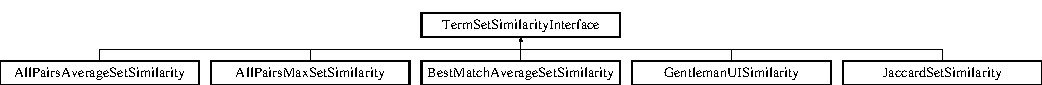
\includegraphics[height=1.137056cm]{classTermSetSimilarityInterface}
\end{center}
\end{figure}
\subsection*{Public Member Functions}
\begin{DoxyCompactItemize}
\item 
virtual double \hyperlink{classTermSetSimilarityInterface_aeb985b714efc3df40e55bdd31e425e04}{calculate\+Similarity} (const boost\+::unordered\+\_\+set$<$ std\+::string $>$ \&termsA, const boost\+::unordered\+\_\+set$<$ std\+::string $>$ \&termsB)=0
\begin{DoxyCompactList}\small\item\em A pure virtual method for calculating term set to term set similarity for sets of \hyperlink{namespaceGO}{GO} terms. \end{DoxyCompactList}\end{DoxyCompactItemize}


\subsection{Detailed Description}
An interface class for comparing semantic similarity of sets of \hyperlink{namespaceGO}{GO} terms. 

This class defines the interface for comparing term set to term set similarity. This is the most useful case for comparing genes with multiple annotations to each other. 

\subsection{Member Function Documentation}
\index{Term\+Set\+Similarity\+Interface@{Term\+Set\+Similarity\+Interface}!calculate\+Similarity@{calculate\+Similarity}}
\index{calculate\+Similarity@{calculate\+Similarity}!Term\+Set\+Similarity\+Interface@{Term\+Set\+Similarity\+Interface}}
\subsubsection[{\texorpdfstring{calculate\+Similarity(const boost\+::unordered\+\_\+set$<$ std\+::string $>$ \&terms\+A, const boost\+::unordered\+\_\+set$<$ std\+::string $>$ \&terms\+B)=0}{calculateSimilarity(const boost::unordered_set< std::string > &termsA, const boost::unordered_set< std::string > &termsB)=0}}]{\setlength{\rightskip}{0pt plus 5cm}virtual double Term\+Set\+Similarity\+Interface\+::calculate\+Similarity (
\begin{DoxyParamCaption}
\item[{const boost\+::unordered\+\_\+set$<$ std\+::string $>$ \&}]{termsA, }
\item[{const boost\+::unordered\+\_\+set$<$ std\+::string $>$ \&}]{termsB}
\end{DoxyParamCaption}
)\hspace{0.3cm}{\ttfamily [pure virtual]}}\hypertarget{classTermSetSimilarityInterface_aeb985b714efc3df40e55bdd31e425e04}{}\label{classTermSetSimilarityInterface_aeb985b714efc3df40e55bdd31e425e04}


A pure virtual method for calculating term set to term set similarity for sets of \hyperlink{namespaceGO}{GO} terms. 

This pure virtual method requires similarity measure to implement the basic interface that returns a similarity value for two sets of go terms. 

Implemented in \hyperlink{classAllPairsMaxSetSimilarity_a0eed3f63e2acdeb8365900b9d7a038c1}{All\+Pairs\+Max\+Set\+Similarity}, \hyperlink{classAllPairsAverageSetSimilarity_a685cd98d44c2e2ab9ee4fe7071066cde}{All\+Pairs\+Average\+Set\+Similarity}, \hyperlink{classBestMatchAverageSetSimilarity_adf1b3109b46f04087f919bdb33e131f0}{Best\+Match\+Average\+Set\+Similarity}, and \hyperlink{classJaccardSetSimilarity_a122a04f7f67b96e393fcde1025a306c3}{Jaccard\+Set\+Similarity}.



The documentation for this class was generated from the following file\+:\begin{DoxyCompactItemize}
\item 
ggtk/Term\+Set\+Similarity\+Interface.\+hpp\end{DoxyCompactItemize}

\hypertarget{classTermSimilarityInterface}{}\section{Term\+Similarity\+Interface Class Reference}
\label{classTermSimilarityInterface}\index{Term\+Similarity\+Interface@{Term\+Similarity\+Interface}}


An interface class for comparing semantic similarity of \hyperlink{namespaceGO}{GO} terms.  




{\ttfamily \#include $<$ggtk/\+Term\+Similarity\+Interface.\+hpp$>$}

Inheritance diagram for Term\+Similarity\+Interface\+:\begin{figure}[H]
\begin{center}
\leavevmode
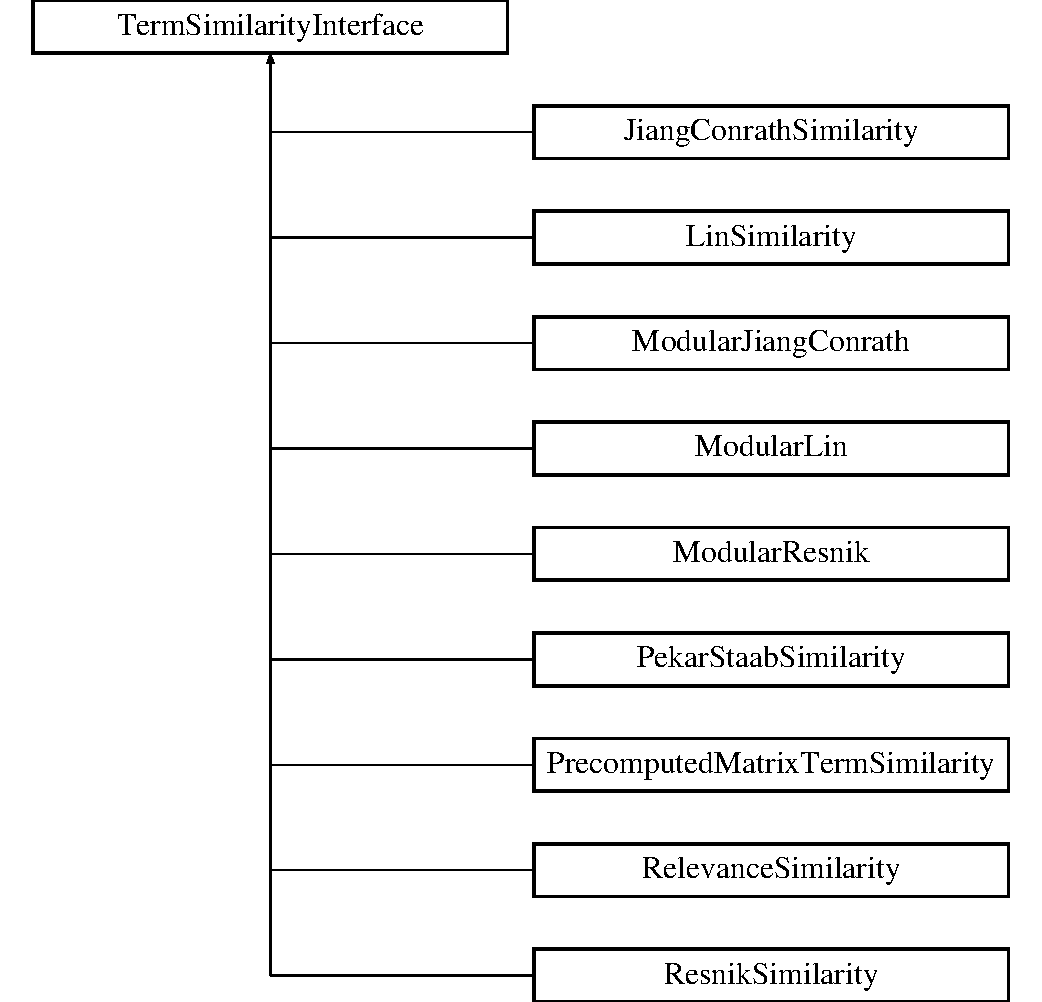
\includegraphics[height=10.000000cm]{classTermSimilarityInterface}
\end{center}
\end{figure}
\subsection*{Public Member Functions}
\begin{DoxyCompactItemize}
\item 
virtual double \hyperlink{classTermSimilarityInterface_ae3474adcfcb02faef65ed5e16ef4db47}{calculate\+Term\+Similarity} (std\+::string go\+TermA, std\+::string go\+TermB)=0
\begin{DoxyCompactList}\small\item\em A pure virtual method for calculating term-\/to-\/term similarity for \hyperlink{namespaceGO}{GO} terms. \end{DoxyCompactList}\item 
virtual double \hyperlink{classTermSimilarityInterface_aa46b7870c7725faab85ec502a3e5242d}{calculate\+Normalized\+Term\+Similarity} (std\+::string go\+TermA, std\+::string go\+TermB)=0
\begin{DoxyCompactList}\small\item\em A pure virtual method for calculating term-\/to-\/term similarity for \hyperlink{namespaceGO}{GO} terms. \end{DoxyCompactList}\end{DoxyCompactItemize}


\subsection{Detailed Description}
An interface class for comparing semantic similarity of \hyperlink{namespaceGO}{GO} terms. 

This class defines the interface for comparing term-\/to-\/term \hyperlink{namespaceGO}{GO} similarity. 

\subsection{Member Function Documentation}
\index{Term\+Similarity\+Interface@{Term\+Similarity\+Interface}!calculate\+Normalized\+Term\+Similarity@{calculate\+Normalized\+Term\+Similarity}}
\index{calculate\+Normalized\+Term\+Similarity@{calculate\+Normalized\+Term\+Similarity}!Term\+Similarity\+Interface@{Term\+Similarity\+Interface}}
\subsubsection[{\texorpdfstring{calculate\+Normalized\+Term\+Similarity(std\+::string go\+Term\+A, std\+::string go\+Term\+B)=0}{calculateNormalizedTermSimilarity(std::string goTermA, std::string goTermB)=0}}]{\setlength{\rightskip}{0pt plus 5cm}virtual double Term\+Similarity\+Interface\+::calculate\+Normalized\+Term\+Similarity (
\begin{DoxyParamCaption}
\item[{std\+::string}]{go\+TermA, }
\item[{std\+::string}]{go\+TermB}
\end{DoxyParamCaption}
)\hspace{0.3cm}{\ttfamily [pure virtual]}}\hypertarget{classTermSimilarityInterface_aa46b7870c7725faab85ec502a3e5242d}{}\label{classTermSimilarityInterface_aa46b7870c7725faab85ec502a3e5242d}


A pure virtual method for calculating term-\/to-\/term similarity for \hyperlink{namespaceGO}{GO} terms. 

This pure virtual method requires similarity measure to implement the basic interface that returns a similarity value for two go terms. This version of the function must be normalzied. Returning similarity between 0 and 1 

Implemented in \hyperlink{classPrecomputedMatrixTermSimilarity_ac2057bd30526a99741c06f8b629b6ae2}{Precomputed\+Matrix\+Term\+Similarity}, \hyperlink{classJiangConrathSimilarity_a489dcbef15f4a5063af79cb03920cdf9}{Jiang\+Conrath\+Similarity}, \hyperlink{classPekarStaabSimilarity_a2de7c29ad8e24467c6b66862320953a1}{Pekar\+Staab\+Similarity}, \hyperlink{classLinSimilarity_a576df5bf234556e57e2ddcfda3d73b93}{Lin\+Similarity}, \hyperlink{classRelevanceSimilarity_ad54bb47157112a225b353c47d1e2fad5}{Relevance\+Similarity}, \hyperlink{classResnikSimilarity_a4e1d6ef4268a905a117fd0c054e4c39b}{Resnik\+Similarity}, \hyperlink{classModularJiangConrath_afbcb95c5f87764de5d33188948f1001b}{Modular\+Jiang\+Conrath}, \hyperlink{classModularLin_a5c4c590808542669e7ba65b60ea8f707}{Modular\+Lin}, and \hyperlink{classModularResnik_aba93eb85400287057037d545e5080265}{Modular\+Resnik}.

\index{Term\+Similarity\+Interface@{Term\+Similarity\+Interface}!calculate\+Term\+Similarity@{calculate\+Term\+Similarity}}
\index{calculate\+Term\+Similarity@{calculate\+Term\+Similarity}!Term\+Similarity\+Interface@{Term\+Similarity\+Interface}}
\subsubsection[{\texorpdfstring{calculate\+Term\+Similarity(std\+::string go\+Term\+A, std\+::string go\+Term\+B)=0}{calculateTermSimilarity(std::string goTermA, std::string goTermB)=0}}]{\setlength{\rightskip}{0pt plus 5cm}virtual double Term\+Similarity\+Interface\+::calculate\+Term\+Similarity (
\begin{DoxyParamCaption}
\item[{std\+::string}]{go\+TermA, }
\item[{std\+::string}]{go\+TermB}
\end{DoxyParamCaption}
)\hspace{0.3cm}{\ttfamily [pure virtual]}}\hypertarget{classTermSimilarityInterface_ae3474adcfcb02faef65ed5e16ef4db47}{}\label{classTermSimilarityInterface_ae3474adcfcb02faef65ed5e16ef4db47}


A pure virtual method for calculating term-\/to-\/term similarity for \hyperlink{namespaceGO}{GO} terms. 

This pure virtual method requires similarity measure to implement the basic interface that returns a similarity value for two go terms. 

Implemented in \hyperlink{classPrecomputedMatrixTermSimilarity_accf2925db5da35cc040f2016813ed631}{Precomputed\+Matrix\+Term\+Similarity}, \hyperlink{classJiangConrathSimilarity_a110fcc0d8b68b6dde9e90d897c859034}{Jiang\+Conrath\+Similarity}, \hyperlink{classPekarStaabSimilarity_a56bb39dcebcf8909f2006d0698f29211}{Pekar\+Staab\+Similarity}, \hyperlink{classModularJiangConrath_a4bb41aa1eced9dd47f4f4c7125a223d5}{Modular\+Jiang\+Conrath}, \hyperlink{classRelevanceSimilarity_a77fd7721c3c98611328f97b6b8c3f9e3}{Relevance\+Similarity}, \hyperlink{classLinSimilarity_a55d2d8bd6aea6fc3e9b0920f05828a15}{Lin\+Similarity}, \hyperlink{classModularLin_a995ef9e4c53b9e96a32259157416df1b}{Modular\+Lin}, \hyperlink{classResnikSimilarity_a340ace5dbdd105847d5fade4c8d20ade}{Resnik\+Similarity}, and \hyperlink{classModularResnik_a78b925c1aadb000d1773ffdacad549df}{Modular\+Resnik}.



The documentation for this class was generated from the following file\+:\begin{DoxyCompactItemize}
\item 
ggtk/Term\+Similarity\+Interface.\+hpp\end{DoxyCompactItemize}

\hypertarget{classTermSimilarityWriter}{}\section{Term\+Similarity\+Writer Class Reference}
\label{classTermSimilarityWriter}\index{Term\+Similarity\+Writer@{Term\+Similarity\+Writer}}


A class write a term similarity matrix to file. Companion to \hyperlink{classPrecomputedMatrixTermSimilarity}{Precomputed\+Matrix\+Term\+Similarity}.  




{\ttfamily \#include $<$ggtk/\+Term\+Similarity\+Writer.\+hpp$>$}

\subsection*{Public Member Functions}
\begin{DoxyCompactItemize}
\item 
\hyperlink{classTermSimilarityWriter_a53dffc62cbc87ba24bc4e10ea0def16c}{Term\+Similarity\+Writer} (\hyperlink{classGoGraph}{Go\+Graph} $\ast$go\+Graph, \hyperlink{classAnnotationData}{Annotation\+Data} $\ast$anno\+Data)
\begin{DoxyCompactList}\small\item\em Parameterized constructor. \end{DoxyCompactList}\item 
void \hyperlink{classTermSimilarityWriter_a6675f612d2f294c2a126576a393b2307}{write\+Similarity\+Matrix} (\hyperlink{classTermSimilarityInterface}{Term\+Similarity\+Interface} $\ast$term\+Sim, std\+::string file\+Name, long ontology\+\_\+code)
\begin{DoxyCompactList}\small\item\em A method to write a term similarity matrix. \end{DoxyCompactList}\item 
void \hyperlink{classTermSimilarityWriter_ab47132660b1a4a2528dff1b97f934b1b}{write\+Similarity\+Matrix\+BP} (\hyperlink{classTermSimilarityInterface}{Term\+Similarity\+Interface} $\ast$term\+Sim, std\+::string file\+Name)
\begin{DoxyCompactList}\small\item\em A method to write a term similarity matrix for Biological Process. \end{DoxyCompactList}\item 
void \hyperlink{classTermSimilarityWriter_ac541f5cb901cece561648acdfa294653}{write\+Similarity\+Matrix\+MF} (\hyperlink{classTermSimilarityInterface}{Term\+Similarity\+Interface} $\ast$term\+Sim, std\+::string file\+Name)
\begin{DoxyCompactList}\small\item\em A method to write a term similarity matrix for Molecular Function. \end{DoxyCompactList}\item 
void \hyperlink{classTermSimilarityWriter_ad021eceaae4427c3e9efea93a63a15ad}{write\+Similarity\+Matrix\+CC} (\hyperlink{classTermSimilarityInterface}{Term\+Similarity\+Interface} $\ast$term\+Sim, std\+::string file\+Name)
\begin{DoxyCompactList}\small\item\em A method to write a term similarity matrix for Cellular Component. \end{DoxyCompactList}\end{DoxyCompactItemize}


\subsection{Detailed Description}
A class write a term similarity matrix to file. Companion to \hyperlink{classPrecomputedMatrixTermSimilarity}{Precomputed\+Matrix\+Term\+Similarity}. 

This class writes a term similarity matrix to file by first calculating all similarity values between pairs of terms. This class will be use to write matrices read by \hyperlink{classPrecomputedMatrixTermSimilarity}{Precomputed\+Matrix\+Term\+Similarity}. 

\subsection{Constructor \& Destructor Documentation}
\index{Term\+Similarity\+Writer@{Term\+Similarity\+Writer}!Term\+Similarity\+Writer@{Term\+Similarity\+Writer}}
\index{Term\+Similarity\+Writer@{Term\+Similarity\+Writer}!Term\+Similarity\+Writer@{Term\+Similarity\+Writer}}
\subsubsection[{\texorpdfstring{Term\+Similarity\+Writer(\+Go\+Graph $\ast$go\+Graph, Annotation\+Data $\ast$anno\+Data)}{TermSimilarityWriter(GoGraph *goGraph, AnnotationData *annoData)}}]{\setlength{\rightskip}{0pt plus 5cm}Term\+Similarity\+Writer\+::\+Term\+Similarity\+Writer (
\begin{DoxyParamCaption}
\item[{{\bf Go\+Graph} $\ast$}]{go\+Graph, }
\item[{{\bf Annotation\+Data} $\ast$}]{anno\+Data}
\end{DoxyParamCaption}
)\hspace{0.3cm}{\ttfamily [inline]}}\hypertarget{classTermSimilarityWriter_a53dffc62cbc87ba24bc4e10ea0def16c}{}\label{classTermSimilarityWriter_a53dffc62cbc87ba24bc4e10ea0def16c}


Parameterized constructor. 

A simple parameterized constructor. This class take an instance of the \hyperlink{namespaceGO}{GO} Graph. 

\subsection{Member Function Documentation}
\index{Term\+Similarity\+Writer@{Term\+Similarity\+Writer}!write\+Similarity\+Matrix@{write\+Similarity\+Matrix}}
\index{write\+Similarity\+Matrix@{write\+Similarity\+Matrix}!Term\+Similarity\+Writer@{Term\+Similarity\+Writer}}
\subsubsection[{\texorpdfstring{write\+Similarity\+Matrix(\+Term\+Similarity\+Interface $\ast$term\+Sim, std\+::string file\+Name, long ontology\+\_\+code)}{writeSimilarityMatrix(TermSimilarityInterface *termSim, std::string fileName, long ontology_code)}}]{\setlength{\rightskip}{0pt plus 5cm}void Term\+Similarity\+Writer\+::write\+Similarity\+Matrix (
\begin{DoxyParamCaption}
\item[{{\bf Term\+Similarity\+Interface} $\ast$}]{term\+Sim, }
\item[{std\+::string}]{file\+Name, }
\item[{long}]{ontology\+\_\+code}
\end{DoxyParamCaption}
)\hspace{0.3cm}{\ttfamily [inline]}}\hypertarget{classTermSimilarityWriter_a6675f612d2f294c2a126576a393b2307}{}\label{classTermSimilarityWriter_a6675f612d2f294c2a126576a393b2307}


A method to write a term similarity matrix. 

Calculates and writes the similarity matrix to file. Calculates the similarity between all pairs of terms. The complexity is O(\+N$^\wedge$2) $\ast$ O(\+Term Pair Calculation Cost). O(\+Term Pair Calculation Cost) is usually near constant time, but some method will be extremely slow and require other methods \index{Term\+Similarity\+Writer@{Term\+Similarity\+Writer}!write\+Similarity\+Matrix\+BP@{write\+Similarity\+Matrix\+BP}}
\index{write\+Similarity\+Matrix\+BP@{write\+Similarity\+Matrix\+BP}!Term\+Similarity\+Writer@{Term\+Similarity\+Writer}}
\subsubsection[{\texorpdfstring{write\+Similarity\+Matrix\+B\+P(\+Term\+Similarity\+Interface $\ast$term\+Sim, std\+::string file\+Name)}{writeSimilarityMatrixBP(TermSimilarityInterface *termSim, std::string fileName)}}]{\setlength{\rightskip}{0pt plus 5cm}void Term\+Similarity\+Writer\+::write\+Similarity\+Matrix\+BP (
\begin{DoxyParamCaption}
\item[{{\bf Term\+Similarity\+Interface} $\ast$}]{term\+Sim, }
\item[{std\+::string}]{file\+Name}
\end{DoxyParamCaption}
)\hspace{0.3cm}{\ttfamily [inline]}}\hypertarget{classTermSimilarityWriter_ab47132660b1a4a2528dff1b97f934b1b}{}\label{classTermSimilarityWriter_ab47132660b1a4a2528dff1b97f934b1b}


A method to write a term similarity matrix for Biological Process. 

Calcualtes and writes the biological process term similarity matrix \index{Term\+Similarity\+Writer@{Term\+Similarity\+Writer}!write\+Similarity\+Matrix\+CC@{write\+Similarity\+Matrix\+CC}}
\index{write\+Similarity\+Matrix\+CC@{write\+Similarity\+Matrix\+CC}!Term\+Similarity\+Writer@{Term\+Similarity\+Writer}}
\subsubsection[{\texorpdfstring{write\+Similarity\+Matrix\+C\+C(\+Term\+Similarity\+Interface $\ast$term\+Sim, std\+::string file\+Name)}{writeSimilarityMatrixCC(TermSimilarityInterface *termSim, std::string fileName)}}]{\setlength{\rightskip}{0pt plus 5cm}void Term\+Similarity\+Writer\+::write\+Similarity\+Matrix\+CC (
\begin{DoxyParamCaption}
\item[{{\bf Term\+Similarity\+Interface} $\ast$}]{term\+Sim, }
\item[{std\+::string}]{file\+Name}
\end{DoxyParamCaption}
)\hspace{0.3cm}{\ttfamily [inline]}}\hypertarget{classTermSimilarityWriter_ad021eceaae4427c3e9efea93a63a15ad}{}\label{classTermSimilarityWriter_ad021eceaae4427c3e9efea93a63a15ad}


A method to write a term similarity matrix for Cellular Component. 

Calcualtes and writes the cellular component term similarity matrix \index{Term\+Similarity\+Writer@{Term\+Similarity\+Writer}!write\+Similarity\+Matrix\+MF@{write\+Similarity\+Matrix\+MF}}
\index{write\+Similarity\+Matrix\+MF@{write\+Similarity\+Matrix\+MF}!Term\+Similarity\+Writer@{Term\+Similarity\+Writer}}
\subsubsection[{\texorpdfstring{write\+Similarity\+Matrix\+M\+F(\+Term\+Similarity\+Interface $\ast$term\+Sim, std\+::string file\+Name)}{writeSimilarityMatrixMF(TermSimilarityInterface *termSim, std::string fileName)}}]{\setlength{\rightskip}{0pt plus 5cm}void Term\+Similarity\+Writer\+::write\+Similarity\+Matrix\+MF (
\begin{DoxyParamCaption}
\item[{{\bf Term\+Similarity\+Interface} $\ast$}]{term\+Sim, }
\item[{std\+::string}]{file\+Name}
\end{DoxyParamCaption}
)\hspace{0.3cm}{\ttfamily [inline]}}\hypertarget{classTermSimilarityWriter_ac541f5cb901cece561648acdfa294653}{}\label{classTermSimilarityWriter_ac541f5cb901cece561648acdfa294653}


A method to write a term similarity matrix for Molecular Function. 

Calcualtes and writes the molecular function term similarity matrix 

The documentation for this class was generated from the following file\+:\begin{DoxyCompactItemize}
\item 
ggtk/Term\+Similarity\+Writer.\+hpp\end{DoxyCompactItemize}

\hypertarget{structGoGraph_1_1VertexProps}{}\section{Go\+Graph\+:\+:Vertex\+Props Struct Reference}
\label{structGoGraph_1_1VertexProps}\index{Go\+Graph\+::\+Vertex\+Props@{Go\+Graph\+::\+Vertex\+Props}}


A Vertex Property object.  




{\ttfamily \#include $<$ggtk/\+Go\+Graph.\+hpp$>$}

\subsection*{Public Member Functions}
\begin{DoxyCompactItemize}
\item 
\hyperlink{structGoGraph_1_1VertexProps_ad60aea44237ee479a4c8768226778590}{$\sim$\+Vertex\+Props} ()
\end{DoxyCompactItemize}
\subsection*{Public Attributes}
\begin{DoxyCompactItemize}
\item 
std\+::string \hyperlink{structGoGraph_1_1VertexProps_a9f3a3e42785bc040b0b827b1ffd3f039}{term\+Id}
\item 
\hyperlink{namespaceGO_a5ae335887b5cf40a9ef3045be9247fc3}{G\+O\+::\+Onto} \hyperlink{structGoGraph_1_1VertexProps_a353631ac064161688da0fb4f458dfcb8}{ontology}
\end{DoxyCompactItemize}


\subsection{Detailed Description}
A Vertex Property object. 

This struct represent the data needed by each vertex. Boost provides constant time access to these members by querying them using the vertex and graph objects (graph\+Var\mbox{[}vertex\mbox{]}.term\+Id ... etc.). 

\subsection{Constructor \& Destructor Documentation}
\index{Go\+Graph\+::\+Vertex\+Props@{Go\+Graph\+::\+Vertex\+Props}!````~Vertex\+Props@{$\sim$\+Vertex\+Props}}
\index{````~Vertex\+Props@{$\sim$\+Vertex\+Props}!Go\+Graph\+::\+Vertex\+Props@{Go\+Graph\+::\+Vertex\+Props}}
\subsubsection[{\texorpdfstring{$\sim$\+Vertex\+Props()}{~VertexProps()}}]{\setlength{\rightskip}{0pt plus 5cm}Go\+Graph\+::\+Vertex\+Props\+::$\sim$\+Vertex\+Props (
\begin{DoxyParamCaption}
{}
\end{DoxyParamCaption}
)\hspace{0.3cm}{\ttfamily [inline]}}\hypertarget{structGoGraph_1_1VertexProps_ad60aea44237ee479a4c8768226778590}{}\label{structGoGraph_1_1VertexProps_ad60aea44237ee479a4c8768226778590}
Desctructor 

\subsection{Member Data Documentation}
\index{Go\+Graph\+::\+Vertex\+Props@{Go\+Graph\+::\+Vertex\+Props}!ontology@{ontology}}
\index{ontology@{ontology}!Go\+Graph\+::\+Vertex\+Props@{Go\+Graph\+::\+Vertex\+Props}}
\subsubsection[{\texorpdfstring{ontology}{ontology}}]{\setlength{\rightskip}{0pt plus 5cm}{\bf G\+O\+::\+Onto} Go\+Graph\+::\+Vertex\+Props\+::ontology}\hypertarget{structGoGraph_1_1VertexProps_a353631ac064161688da0fb4f458dfcb8}{}\label{structGoGraph_1_1VertexProps_a353631ac064161688da0fb4f458dfcb8}
The ontology of the \hyperlink{namespaceGO}{GO} term, BP, MF, CC \index{Go\+Graph\+::\+Vertex\+Props@{Go\+Graph\+::\+Vertex\+Props}!term\+Id@{term\+Id}}
\index{term\+Id@{term\+Id}!Go\+Graph\+::\+Vertex\+Props@{Go\+Graph\+::\+Vertex\+Props}}
\subsubsection[{\texorpdfstring{term\+Id}{termId}}]{\setlength{\rightskip}{0pt plus 5cm}std\+::string Go\+Graph\+::\+Vertex\+Props\+::term\+Id}\hypertarget{structGoGraph_1_1VertexProps_a9f3a3e42785bc040b0b827b1ffd3f039}{}\label{structGoGraph_1_1VertexProps_a9f3a3e42785bc040b0b827b1ffd3f039}
The term id of the go term, the \hyperlink{namespaceGO}{GO} accession, \hyperlink{namespaceGO}{GO}\+:\#\#\#\#\#\#\#\#. 

The documentation for this struct was generated from the following file\+:\begin{DoxyCompactItemize}
\item 
ggtk/Go\+Graph.\+hpp\end{DoxyCompactItemize}

%--- End generated contents ---

% Index
\backmatter
\newpage
\phantomsection
\clearemptydoublepage
\addcontentsline{toc}{chapter}{Index}
\printindex

\end{document}
